% TEX-PROGRAM: PDFLATEX

% TIPO DE DOCUMENTO

\documentclass[14pt,twoside,final]{extbook} % Opciones: draft (borrador) y final (imprimatur)

% CODIFICACIÓN DE ARCHIVO Y FUENTE

\usepackage[utf8]{inputenc}
\usepackage[TS1,T1]{fontenc}

% SÍMBOLOS

\usepackage[full]{textcomp} % PDFLATEX

% IDIOMA

\usepackage[american,spanish,mexico,es-noindentfirst,es-nosectiondot]{babel}

% Opciones:

% Ordinales: "a, "A, "o, "O, "er, "ER 
% Cedilla: "c, "C
% Erre: "rr, "RR. rr, pero -r cuando se divide
% División silábica: "- Como \- pero permite más divisiones. "= Como - pero permite más divisiones. "~ guion estilístico. "+, "+-, "+-- como -, -- y ---, pero sin división. ~-, ~-- y ~--- lo mismo que lo anterior. "" permite más divisiones, antes y después. "/ una barra un poco más baja (línea base).
% \sptext{texto} activa las voladitas. Ejemplo: 1\sptext{a} edición.
% \lsc{texto} pasa texto a versalitas. Ejemplo: \lsc{XX}, \lsc{ONU}, etc.

% TIPOGRAFÍA COCHINEAL

\usepackage[sups]{cochineal} % Version: 1.076
\useosf
\useproportional
\usepackage[cochineal,vvarbb]{newtxmath} % Soporte matemático

% Opciones:

% scale o scaled = escalará la fuente
% p o proportional = usará números proporcionales
% lf o lining = usará números alineados
% osf u oldstyle = usará números antiguos
% sups = usará superiores en vez de los marcadores predeterminados de LaTeX
% swashQ = usará la Q con cola larga
% scosf = usará siempre números antiguos en un bloque de versalitas

% Uso local:

% \textsu{1234567890} produce superíndices
% {\sufigures } produce superíndices
% \textin{1234567890} produce subíndices
% {\infigures } produce subíndices
% \textde{1234567890} produce denominadores
% {\defigures } produce denominadores
% \textfrac[2]{63}{64} produce fracciones vulgares
% \textcircled{w} encierra en círculos letras y números
% \textlf{1234567890} produce números alineados
% {\lfstyle } produce números alineados
% \texttlf{1234567890} produce números tabulares alineados
% {\tlfstyle } produce números tabulares alineados
% \textosf{1234567890} produce números antiguos
% {\osfstyle } produce números antiguos
% \texttosf{1234567890} produce números tabulares antiguos
% {\tosfstyle } produce números tabulares antiguos

% ADORNOS

\usepackage{shapepar} % Para el colofón
\usepackage{calligra} % Para el nombre de José Antonio Villegas

% SANGRIA

\usepackage{hanging} % Para la bibliografía

% Espacio horizontal entre el marcador y la primera letra en las notas a pie de página.

\let\oldfootnote\footnote
\renewcommand\footnote[1]{%
\oldfootnote{\hspace{1mm}#1}}

% Recomendación de Robert Bringhurst en notas a pie de página

\makeatletter
\renewcommand\@makefntext[1]{%
\setlength\parindent{1.5em}% 1.5em by default
\indent
\mbox{\@thefnmark\hspace*{0.5em}}{#1}}% 0.5em by default
\makeatother

% CITAS A CUERPO DE TEXTO

\let\quoting\relax\let\endquoting\relax % Arreglo para los paquetes quoting y babel

\usepackage{kvoptions} % Sine qua non para el paquete quoting
\usepackage[indentfirst=false,noorphans=true,vskip=14pt]{quoting} % Alternativa a quotation y quote pues mejora los espacios en blanco, antes y después de los párrafos

% INDICE DE CONTENIDOS

\usepackage{titletoc}

% Índice de contenido (Estilo Robert Bringhurst)
% \textbullet punto de separación entre el título y la página 

\titlecontents{chapter}[2.25em]{}% Por defecto 2.25em
{\contentslabel{2.25em}}{}% Por defecto 2.25em
{\hspace{0.5em}{\textbullet}\hspace{0.5em}{\thecontentspage}}
\titlecontents{section}[3.45em]{}% Por defecto 3.45em
{\contentslabel{2.25em}}{}%
{\hspace{0.5em}{\textbullet}\hspace{0.5em}{\thecontentspage}}
\titlecontents{subsection}[5em]{}%
{\contentslabel{2.25em}}{}%
{\hspace{0.5em}{\textbullet}\hspace{0.5em}{\thecontentspage}}
\titlecontents{subsubsection}[5em]{}%
{\contentslabel{2.25em}}{}%
{\hspace{0.5em}{\textbullet}\hspace{0.5em}{\thecontentspage}}

% Índice de figuras (Estilo Robert Bringhurst)

\titlecontents{figure}[2.25em]{}%
{\contentslabel{2.25em}}{}%
{\hspace{0.5em}{\textbullet}\hspace{0.5em}{\thecontentspage}}

% Índice de Cuadros (Estilo Robert Bringhurst)

\titlecontents{table}[2.25em]{}%
{\contentslabel{2.25em}}{}%
{\hspace{0.5em}{\textbullet}\hspace{0.5em}{\thecontentspage}}

% INDICES

\usepackage{imakeidx} % Analítico, onomástico, toponímico, etc. Opciónes: makeindex, intoc

\makeindex[title=Índice onomástico,name=nombres,columns=2,intoc,options=-s nombres.mst]
\makeindex[title=Índice toponímico,name=lugares,columns=2,intoc,options=-s lugares.mst]
%\makeindex[title=Índice analítico,name=analitico,columns=2,intoc]

% Elimina el número de página en la primera hoja de los índices ya que imakeidx usa plain pagestyle.

\makeatletter
\renewcommand\ps@plain{%  
\renewcommand\@oddfoot{}%
\renewcommand\@oddhead{}%
}
\makeatother

% PARCHES PARA LATEX

\usepackage{etoolbox} % Remueve negritas del Índice General, excepto el título. Hack para el paquetes imakeidx.

% Remueve 'Capítulo N' al principio de cada capítulo.

% \Huge \mdseries #1\par\nobreak <--- Default
% \Large \centering\mdseries\sc #1\par\nobreak <--- Hacking (smallcaps)
% \scshape pone los títulos en versalitas negritas (LaTeX). \sc desactiva las negritas porque es una instrucción primitiva de TeX.

\makeatletter
\def\@makechapterhead#1{%
  \vspace*{50\p@}%
  {\parindent \z@ \raggedright \normalfont
    \interlinepenalty\@M
    \Large \centering\bfseries\sc #1\par\nobreak
    \vskip 40\p@
  }}
\def\@makeschapterhead#1{%
  \vspace*{50\p@}%
  {\parindent \z@ \raggedright \normalfont
    \interlinepenalty\@M
    \Large \centering\bfseries\sc #1\par\nobreak
    \vskip 40\p@
  }}
\makeatother

\makeatletter
\patchcmd{\l@chapter}{\bfseries}{}{}{}
\makeatother

% Sección

\makeatletter
\renewcommand\section{\@startsection {section}{1}{\z@}%
                                     {-3.5ex \@plus -1ex \@minus -.2ex}%
                                     {2.3ex \@plus .2ex}%
                                     {\normalfont\large\bfseries\sc}}
\makeatletter

\makeatletter
\patchcmd{\l@section}{\bfseries}{}{}{}
\makeatother

% Subsección

\makeatletter
\renewcommand\subsection{\@startsection {subsection}{2}{\z@}%
                                        {1.5ex \@plus -1ex \@minus -.2ex}%
                                        {1.5ex \@plus .2ex}%
                                        {\normalfont\large\bfseries\sc}} 
\makeatother

\makeatletter
\patchcmd{\l@section}{\bfseries}{}{}{}
\makeatother

% Subsubsection

\makeatletter
\renewcommand\subsubsection{\@startsection {subsubsection}{3}{\z@}%
                                           {1.5ex \@plus -1ex \@minus -.2ex}%
                                           {1.5ex \@plus .2ex}%
                                           {\normalfont\large\bfseries\sc}}
\makeatother

\makeatletter
\patchcmd{\l@section}{\bfseries}{}{}{}
\makeatother

% Incrementa los espacios de las secciones en el Índice.

\makeatletter
\pretocmd{\chapter}{\addtocontents{toc}{\protect\addvspace{15\p@}}}{}{}
\pretocmd{\section}{\addtocontents{toc}{\protect\addvspace{5\p@}}}{}{}
\makeatother

% APÉNDICES

\usepackage{appendix}

% MICROTIPOGRAFÍA

\usepackage[activate={true,nocompatibility},final=true,babel=true,tracking=true,
kerning=true,spacing=false,factor=1100,stretch=20,shrink=20]{microtype} % kerning=true pdftex
\SetTracking[no ligatures=q]{encoding=*,shape=sc}{30} % Elimina ligaduras, kerning.
%\DeclareMicrotypeSet*{smallcapsi} % Kerning versalitas itálicas
%{encoding={TS1,T1},shape={sc*,si,scit}}

% DISPOSICIÓN TIPOGRÁFICA

\usepackage[letterpaper,includehead,headsep=1.5cm,left=4cm,right=3cm,top=3cm,bottom=3cm]{geometry} % Márgenes (Tamaño carta)

% HERRAMIENTAS DE DISEÑO

\usepackage{eso-pic} % Cuadrícula. Opciones: "grid" agrega una cuadrícula. gridBG=true,gridcolor=blue
%\usepackage{showframe} % Elementos macrotipográficos
%\usepackage[switch*]{lineno} % Números de líneas en párrafos
%\usepackage{fnlineno} % Números de lineas en notas a pie de páginas
%\linenumbers % Agrega números de lineas. Activar con lineno
%\renewcommand\thelinenumber{\color{blue}\arabic{linenumber}} % Agrega color a las líneas
%\usepackage[columns=2,headings=false,margin=false]{typogrid} % Draw a grid on the page.
%\usepackage{fonttable}

% ENCABEZADOS

\usepackage[nocheck]{fancyhdr} % Encabezados personalizados. Opciones: nocheck,compatV3

% PÁGINA EN BLANCO

\usepackage{emptypage} % Página en blanco

% LISTAS NUMERADAS

\usepackage{enumitem} % opciones: inline para crear las listas dentro del texto principal.

% GRÁFICOS

\usepackage[pdftex]{graphicx} % Gráficos. Opción: pdftex, luatex
\graphicspath{{images/}} % Almacenamiento (imágenes).
\usepackage{tikz,xcolor} % Color
\usepackage{pgfplots} % Graficos de barras, logarítmico, etc
\pgfplotsset{compat=newest}
\usepackage{pgf-pie} % Diagramas de pastel
\usepackage{soulutf8} % Arreglo para el paquete soul.
\sethlcolor{red} % Color rojo para el marca textos.
\usepackage{silence} % Necesario para suprimir el mensaje del paquete everypage
\WarningsOff[everypage] % Elimina el mensaje
\usepackage{transparent} % transparencia en imágenes
\usepackage{tcolorbox} % Cajas de diálogo.
%\usepackage[stamp=true,text=Borrador]{draftwatermark} % Marca al agua (borrador)
\usepackage[normalem]{ulem} % Tachado de palabras

% TABLAS

\usepackage{siunitx}
\usepackage{longtable,booktabs}
\usepackage{multirow}
\usepackage{rotating}
\usepackage{float}
\usepackage[tablename=Cuadro,figurename=Imagen,font=small]{caption}
\usepackage[enum,lineno]{tabfigures} % Mejora los números en toc, enum y lineno.

% UTILIDADES PARA PDF

\usepackage{pdfpages} % Inserta archivos PDF. Necesario para la portada.

% PDF para pantalla (Día y noche)

% Color ahuesado (Día)

%\definecolor{ahuesado}{RGB}{255 255 224} % Definimos nuestro color (ahuesado, por defecto).
%\pagecolor{ahuesado} % Según estudios científicos, el color ahuesado es el ideal para leer un PDF en pantalla por el día.

% Color durazno (Noche)

%\definecolor{durazno}{RGB}{255 218 185} % Definimos nuestro color (Durazno, por defecto).
%\pagecolor{durazno} % Según estudios científicos, el color durazno es el ideal para leer un PDF en pantalla por la noche.

% METADATOS PDF

\usepackage{hyperxmp}

% ENLACES DINÁMICOS

\usepackage{url} % Direcciones de Internet
\urlstyle{rm} % Desactiva las fuentes monoespaciadas y usa las romanas.
\usepackage{keyval} % Sine qua non para hyperref. Activa los boleanos.
\usepackage[pdftex,unicode,hyperindex=true,final=true,bookmarks=true,
bookmarksnumbered=true,bookmarksopen=true,breaklinks=true,citecolor=black,
colorlinks=true,linkcolor=black,urlcolor=black,pdftitle={Familia y poder en el centro de Veracruz. Los Villegas de Jalacingo, 1872-1910},pdfsubject={Tesis Maestría en Historia},pdfauthor={Noel Merino Hernández},pdfkeywords={Familia Poder Veracruz Villegas Jalacingo Historia},pdfproducer={pdflatex 3.14159265-2.6-1.40.21 (TeX Live 2020/Debian)},pdfcreator={Tuxkernel (muxkernel@gmail.com)}]{hyperref} % Opción: pdftex, luatex, unicode (luatex)
\providecommand\phantomsection{} % Necessary for seudo chapters

% COPYRIGHT

\hypersetup{
pdfcopyright={© 2007-2023. Noel Merino Hernández. Algunos derechos reservados. Este documento se proporciona como es, sin ningún tipo de garantía, aunque se espera que pueda ser útil, y se distribuye bajo una licencia Creative Commons Atribución 4.0 Internacional (CC BY 4.0). Por lo tanto, eres libre de compartir, copiar y redistribuir el material en cualquier medio o formato. Adaptar, remezclar, transformar y construir a partir del material para cualquier propósito, incluso comercialmente. El licenciante no puede revocar estas libertades en tanto usted siga los términos de la licencia, bajo los siguientes términos: Atribución. Usted debe dar crédito de manera adecuada, brindar un enlace a la licencia, e indicar si se han realizado cambios. Puede hacerlo en cualquier forma razonable, pero no de forma tal que sugiera que usted o su uso tienen el apoyo del licenciante. No hay restricciones adicionales. No puede aplicar términos legales ni medidas tecnológicas que restrinjan legalmente a otras a hacer cualquier uso permitido por la licencia. Avisos: Usted no tiene que cumplir con la licencia para elementos del material en el dominio público o cuando su uso esté permitido por una excepción o limitación aplicable. No se dan garantías. La licencia podría no darle todos los permisos que necesita para el uso que tenga previsto. Por ejemplo, otros derechos como publicidad, privacidad, o derechos morales pueden limitar la forma en que utilice el material.},
pdflicenseurl={https://creativecommons.org/licenses/by/4.0/deed.es},
}

% IMPRENTA Y ARCHIVADO

%\usepackage[a-1b]{pdfx} % Archivado

% LA DIVERSIÓN COMIENZA AQUÍ ;-) (SANGRE, SUDOR Y LÁGRIMAS)

% DOCUMENTO

\raggedbottom % Reduce los espacios en blanco en cada hoja y los envía al final.
%\flushbottom % Distribuye los espacios en blanco en cada hoja de forma aleatoria.
\newcommand{\nota}[1]{\marginpar{\color{blue}\tiny #1}}% Nota al margen
\begin{document}
\pagenumbering{arabic}
\setcounter{page}{1}
\parindent=5mm % Sangría.
\parskip=0mm % Espacio entre párrafos.
%\setlength{\footnotesep}{0pt} % Elimina el espacio vertical entre las notas a pie de página.
%\linespread{1.5} % Interlineado
% PORTADA
\newpage
\thispagestyle{empty}
\protect\phantomsection
\addcontentsline{toc}{chapter}{Portada}
\addtocontents{toc}{\vspace{\normalbaselineskip}} % Add some vertical space between titles in TOC
\begin{center}
\begin{minipage}{11cm}
\includegraphics[width=3cm]{buap}\label{fig:buap} \hfill \includegraphics[width=2.8cm]{icsyh}
\label{fig:icsyh}
\end{minipage}
\end{center}
\protect\smallskip
\begin{center}
\large\scshape Benemérita Universidad Autónoma de Puebla
\end{center}
\begin{center}
\large\scshape Instituto de Ciencias Sociales y Humanidades «Alfonso Vélez Pliego»
\end{center}
\begin{center}
\large\scshape Posgrado en Historia
\end{center}
\protect\bigskip
\begin{center}
\Large\itshape Familia y poder en el centro de Veracruz. \\ Los Villegas de Jalacingo, 1872--1910
\end{center}
\protect\bigskip
\begin{center}
\Large\scshape tesis
\end{center}
\protect\bigskip
\begin{center}
que para obtener el grado de:
\end{center}
\begin{center}
\scshape Maestro en Historia
\end{center}
\begin{center}
Presenta:
\end{center}
\begin{center}
\scshape Lic. Noel Merino Hernández
\end{center}
\begin{center}
Directora:
\end{center}
\begin{center}
\scshape Dra. Leticia Gamboa Ojeda
\end{center}
\protect\medskip
\begin{center}
Puebla, Pue., 29 de agosto del 2007
\end{center}
\begin{center}
(núm.\ 64)
\end{center}
% LICENCIA DO WHAT THE FUCK YOU WANT TO PUBLIC LICENSE
\newpage
\thispagestyle{empty}
\protect\phantomsection
\addcontentsline{toc}{chapter}{Licencia \texorpdfstring{\textsc{wtfpl}}{WTFPL}}
\addtocontents{toc}{\vspace{\normalbaselineskip}} % Add some vertical space between titles in TOC
\vspace*{0pt}
\vfill
\begin{scriptsize}
\begin{flushleft}
\begin{minipage}{7.5cm}
\includegraphics[width=2.5cm]{wtfpl-large}\phantomsection\label{fig:wtfpl-large} \protect\medskip

\includegraphics[width=2.5cm]{wtfpl}\phantomsection\label{fig:wtfpl} \protect\medskip

\def\fileversion{1.042}
\def\filedate{(22-01-2024)}
\href{https://tuxkernel.github.io/tx/dl/cv.txt}{versión\space\fileversion\space\filedate} \protect\medskip

\textcopyright\ 2007--2024. \href{noel_merino@yahoo.com.mx}{Noel Merino Hernández} (del texto).

\textcopyright\ 2022--2024. \href{muxkernel@gmail.com}{Tuxkernel} (de la composición tipográfica). \protect\medskip

Este documento se proporciona \emph{como es,} sin ningún tipo de garantía, aunque se espera que pueda ser útil, y se distribuye bajo \href{http://www.wtfpl.net/}{Do What The Fuck You Want To Public License (\lsc{WTFPL})}, versión 2.0 o posterior. Por lo tanto, todos son absolutamente libres de hacer de este documento lo que quieran. \protect\medskip

Para más información sobre esta licencia, visita: \protect\medskip

\textbf{\url{http://www.wtfpl.net/about/}}
\end{minipage}
\end{flushleft}
\end{scriptsize}
% DEDICATORIA
\newpage
\pagestyle{empty}
\phantomsection
\addcontentsline{toc}{chapter}{Dedicatoria}
\vspace*{48pt}
\begin{flushright}
\textit{Francisco R. Córdoba Olivares}
\end{flushright}
\begin{flushright}
\textsc{In memoriam}
\end{flushright}
\protect\smallskip
\begin{flushright}
\textit{A mis padres y hermanos, con cariño.}
\end{flushright}
% PÁGINA EN BLANCO
\newpage
\pagestyle{empty}
% NOTA PRELIMINAR
\newpage
\pagestyle{empty}
\chapter*{Nota preliminar}
\label{ch:nota-preliminar}
\addcontentsline{toc}{chapter}{Nota preliminar}
Insatisfecho con la formación que se hizo en 2007, he realizado una «nueva» versión con cambios \emph{únicamente} en la composición tipográfica, ya que el texto y el contenido son ---con ligeras modificaciones---, en esencia, los mismos. El texto original (2007) aún puede consultarse en la siguiente dirección electrónica:
\begin{center}
\href{https://tuxkernel.github.io/tx/dl/thesis-2007.pdf}{\bfseries https://tuxkernel.github.io/tx/dl/thesis-2007.pdf}
\end{center}
la nueva (2024) en:
\begin{center}
\href{https://tuxkernel.github.io/tx/dl/thesis-2024.pdf}{\bfseries https://tuxkernel.github.io/tx/dl/thesis-2024.pdf}
\end{center}
No importa que sean versiones distintas de un mismo texto, cualquiera es válida para fines académicos. Sin embargo, al utilizar la «nueva» versión, deberás colocar en tus notas algo como lo siguiente:
\begin{center}
\bfseries (Merino, 2024 [2007], p. 13)
\end{center}
\noindent Lo anterior indica que estas citando la página 13 de la versión 2024, pero cuyo contenido está basado en la de 2007; solo adapta el ejemplo anterior a tu modelo de citación. Si te resulta «compleja» esta nueva modalidad para citar, usa la versión «original» (2007) y listo.

El texto de 2007 está plagado de errores sintácticos, ortotipográficos e incluso hermenéuticos. Me hubiera gustado corregirlos ese año, pero en los posgrados de «calidad» \textsc{conacyt}, o te dedicas a escribir para titularte en tiempo y forma, o a corregir pero con una titulación extemporánea. ¡Así de simple! Corregirlos en la «nueva» versión habría implicado pasar por alto el texto primigenio, perdiendo así su «originalidad». ¡Caveat emptor!

Agradezco a \href{muxkernel@gmail.com}{Tuxkernel} su tiempo, paciencia y dedicación para \emph{componer} nuevamente el texto.
% AGRADECIMIENTOS
\chapter*{Agradecimientos}
\label{ch:agradecimientos}
\thispagestyle{empty}
\pagestyle{fancy}
\fancyhf{} % Remueve encabezados y pies previos. Necesario sí o sí.
\fancyhead[CE,CO]{\small\sc agradecimientos} % Centrados
\fancyhead[LE,RO]{\thepage}
\renewcommand{\headrulewidth}{0pt}
\addcontentsline{toc}{chapter}{Agradecimientos}
\addtocontents{toc}{\vspace{\normalbaselineskip}}
La paternidad de este trabajo no es exclusivamente mía. Fueron demasiadas las personas que contribuyeron en su nacimiento que un recuento de ellos me obligaría a escribir un texto gordo, casi con las mismas características de éste. Tampoco estableceré grados de apoyo pues cada uno contribuyó según sus tiempos y dedicación.

Es paradójico que quienes más contribuyen y viven a ras de suelo en ese maravilloso país de la historia, son quizá, los menos recordados. Este trabajo rescata del olvido sus nombres y les otorga un lugar especial en la historia. En este sentido, agradezco a Guadalupe Rivas Romero, encargada de la biblioteca «Ernesto de la Torre Villar» del Instituto de Ciencias Sociales y Humanidades «Alfonso Vélez Pliego», sus finas atenciones. En varias ocasiones tuvo que arriesgar el pellejo a guisa de regaños y coscorrones por haberme facilitado materiales no siempre para su consulta en casa.

Al Mtro. Masae Suwagara Hikichi, director de la misma, le estoy infinitamente agradecido por su presunta complicidad y confabulación también en estos hechos. Reconozco públicamente el eficiente trabajo que desempeña María Magdalena Olivares Molina en todos los asuntos administrativos de la maestría y el buen trato siempre mostrado hacia mi persona.

Al Ing. Heber H. Salazar Roldán y al Lic. Jesús Rodríguez Fernández de Lara, por proporcionarme toda la infraestructura informática del Instituto. Aunque comparto con ellos el gusto por las microcomputadoras y los sistemas operativos, no hemos coincidido aún sobre el uso del \emph{software} propietario y el \emph{software} libre. A todos los maestros y maestras del Instituto, especialmente a los doctores David LaFrance, Miguel Ángel Cuenya Mateos, John Mraz Sikes, Rosalina Estrada Urroz, Lilián Illades Aguiar y Osvaldo Tamain Rossi. Todos ellos son culpables de mi buena formación académica. Al Mtro. Agustín Grajales Porras, director del Instituto de Ciencias Sociales y Humanidades «Alfonso Vélez Pliego» de la Benemérita Universidad Autónoma de Puebla, por todo el apoyo recibido. Al Mtro. Roberto Vélez Pliego, coordinador del Posgrado en Historia; a los doctores Ricardo Téllez Girón-López y Abel Juárez Martínez, por la lectura, sugerencias y críticas al texto. Al Dr. José Manuel Velasco Toro, profesor-investigador del Instituto de Investigaciones Histórico-Sociales de la Universidad Veracruzana, por permitirme utilizar información previamente consultada por él, proveniente del Archivo General del Estado de Veracruz sobre el cantón de Jalacingo.

A todo el personal que labora en el Archivo General de Notarías del Estado de Puebla. Especialmente a \emph{toñita,} quien me condujo en las profundidades de ese acervo.

En Jalacingo, agradezco al Lic. Euclides Librado Sarmiento, encargado de la oficina del Registro Público y de la Propiedad; así como a Elizabeth Gamino Jiménez y Silvestre Estudillo García, por haberme proporcionado todo el material para elaborar esta tesis. Les recuerdo que amenazo con volver muy pronto.

Por segunda ocasión, agradezco al Consejo Nacional de Ciencia y Tecnología (\textsc{conacyt}). Su beca no sólo me permitió engordar algunos kilos, sino también hacerme de varias centenas de libros.

En Puebla, agradezco la amistad que me brindaron Mariano Castellanos Arenas, Ricardo F. Macip Ríos, Iván Gerardo González Nolasco, Vanessa Álvarez Guzmán, Lilián González Torres y Jesús Guevara Martínez. De las infinitas charlas que he tenido con ellos, han surgido proyectos y no pocas discusiones.

A toda mi familia que reside en Puebla. A mis tías Guille y Rosy; a mis primos Bety, Andy, Jessy y la pequeña Paola, con quienes recorrí en varias ocasiones el valle de Perote.

A los camaradas y compañeros de la maestría; Jesús Arturo Filigrana Rosique, Claudia Elena García Marañón, Angélica Olea Prieto, Esther Cuatzon Mora, Leticia Villalobos Sampayo y Lourdes Guevara Lázaro. Ustedes saben que los llevo en la piel. A Edmundo Hernández Amador y Jorge Osbaldo Zúñiga Cárdenas, ahora mis hermanos, por emprender juntos esta temeraria aventura.

A la Dra. Leticia Gamboa Ojeda, una directora tan ruda como técnica, que con máscara y cabellera se lanzó al cuadrilátero para dirigir la tesis. Ella no es culpable de las malas interpretaciones, omisiones ortográficas y terquedades de este texto. Finalmente a mis padres y hermanos, a quienes espero resarcir con este trabajo, mi ausencia en los últimos meses.
\cleardoublepage
% CONTENIDO
\makeatletter
\renewcommand\@dotsep{200} % Remueve los puntos en los índices
\makeatother
\renewcommand{\contentsname}{Índice de contenidos}
\thispagestyle{empty}
\pagestyle{fancy}
\fancyhf{} % Remueve los encabezados y pies previos. Necesario sí o sí.
\fancyhead[CE,CO]{\small\sc índice de contenidos} % Centrados
\fancyhead[RO,LE]{\thepage}
\fancyfoot{}
\renewcommand{\headrulewidth}{0pt}
\microtypesetup{protrusion=false}
\protect\phantomsection
\addcontentsline{toc}{chapter}{Índice de contenidos}
\tableofcontents
\microtypesetup{protrusion=true}
\cleardoublepage
% ÍNDICE DE CUADROS
\makeatletter
\renewcommand\@dotsep{200} % Remueve los puntos en los índices
\makeatother
\renewcommand{\listtablename}{Índice de cuadros}
\microtypesetup{protrusion=false}
\listoftables
\microtypesetup{protrusion=true}
\thispagestyle{empty}
\pagestyle{fancy}
\fancyhf{} % Remueve los encabezados y pies previos. Necesario sí o sí.
\fancyhead[CE,CO]{\small\sc índice de cuadros} % Centrados
\fancyhead[RO,LE]{\thepage}
\fancyfoot{}
\renewcommand{\headrulewidth}{0pt}
\addcontentsline{toc}{chapter}{Índice de cuadros}
% ÍNDICE DE FIGURAS
\makeatletter
\renewcommand\@dotsep{200} % Remueve los puntos en los índices
\makeatother
\renewcommand{\listfigurename}{Índice de imágenes}
\microtypesetup{protrusion=false}
\listoffigures
\microtypesetup{protrusion=true}
\thispagestyle{empty}
\pagestyle{fancy}
\fancyhf{} % Remueve los encabezados y pies previos. Necesario sí o sí.
\fancyhead[CE,CO]{\small\sc índice de imágenes} % Centrados
\fancyhead[RO,LE]{\thepage}
\fancyfoot{}
\renewcommand{\headrulewidth}{0pt}
\addcontentsline{toc}{chapter}{Índice de imágenes}
% SIGLAS Y ABREVIATURAS
\chapter*{Siglas y abreviaturas}
\label{ch:siglas-y-abreviaturas}
\pagestyle{empty}
\thispagestyle{empty}
\pagestyle{fancy}
\fancyhf{} % Remueve los encabezados y pies previos. Necesario sí o sí.
\fancyhead[CE,CO]{\small\sc siglas y abreviaturas} % Centrados
\fancyhead[RO,LE]{\thepage}
\renewcommand{\headrulewidth}{0pt}
\addcontentsline{toc}{chapter}{Siglas y abreviaturas}
\begin{table}[H]
\centering
\begin{tabular}{@{}ll@{}}
\textsc{acam} & Archivo de la Comisión Agraria Mixta \\
\textsc{agev} & Archivo General del Estado de Veracruz \\
\textsc{agnep} & Archivo General de Notarías del Estado de Puebla \\
\textsc{apj} & Archivo Parroquial de Jalacingo \\
\textsc{arppj} & Archivo del Registro Público y de la Propiedad de Jalacingo \\
\textsc{asgg} & Archivo de la Secretaría General de Gobierno \\
\textsc{gyj} & Gobernación y Justicia \\
\textsc{f} & Fomento \\
c. & caja \\
Dip. prop. & Diputado propietario \\
enc. & encargado \\
exp. & expediente \\
f. & folio \\
fs. & folios \\
Inst. & Instrumento \\
Pdte. & Presidente \\
Prot. & Protocolo \\
Sec. & Sección \\
Sem. & Semestre \\
Srio. & secretario \\
\end{tabular}
\label{tab:siglas-y-abreviaturas}
\end{table}
% SÍMBOLOS
\chapter*{Símbolos}
\label{ch:simbolos}
\pagestyle{empty}
\thispagestyle{empty}
\pagestyle{fancy}
\fancyhf{} % Remueve los encabezados y pies previos. Necesario sí o sí.
\fancyhead[CE,CO]{\small\sc símbolos} % Centrados
\fancyhead[RO,LE]{\thepage}
\renewcommand{\headrulewidth}{0pt}
\addcontentsline{toc}{chapter}{Símbolos}
\begin{table}[H]
\centering
\begin{tabular}{@{}ll@{}}
@ & arrobas \\
¢ & centavos \\
°C & grados celsius \\
ha & hectáreas \\
hl & hectolitros \\
hp & caballos de fuerza \\
kg & kilogramos \\
km & kilómetros \\
km\textsu{2} & kilómetros cuadrados \\
l & litros \\
m & metros \\
m\textsu{2} & metros cuadrados \\
\% & tanto por ciento o porcentaje \\
\$ & pesos \\
W & watts \\
\end{tabular}
\label{tab:simbolos}
\end{table}
\cleardoublepage
% EPIGRAFE
\newpage
\pagestyle{empty}
\pdfbookmark{Epígrafes (Bloch-Certeau)}{bloch-certeau}
\begin{flushright}
\begin{minipage}{8cm}
\emph{Cuidémonos de quitar a nuestra ciencia su parte de poesía. Cuidémonos, sobre todo \emph{[...]}, de sonrojarnos por ello. Sería una formidable tontería pensar que por tan poderoso atractivo sobre la sensibilidad, tiene que ser menos capaz también de satisfacer a nuestra inteligencia.}
\end{minipage}
\end{flushright}
\begin{flushright}
\textsc{Marc Bloch}\index[nombres]{Bloch, Marc}
\end{flushright}
\protect\smallskip
\begin{flushright}
\begin{minipage}{8cm}
\emph{Nuestros queridos muertos entran en el texto porque no pueden \emph{[...]} hablarnos \emph{[...]}. Los fantasmas se meten en la escritura, sólo cuando callan para siempre \emph{[...]}. La búsqueda histórica del \guilsinglleft sentido\guilsinglright{}, no es sino la búsqueda del \emph{Otro,} pero esta acción contradictoria trata de envolver y ocultar en el «sentido» la alteridad de este extraño, o, lo que es lo mismo, trata de calmar a los muertos que todavía se aparecen y ofrecerles tumbas escriturísticas.}
\end{minipage}
\end{flushright}
\begin{flushright}
\textsc{Michel de Certeau}\index[nombres]{Certeau, Michel de}
\end{flushright}
% INTRODUCCIÓN
\chapter*{Introducción}
\label{ch:introduccion}
\pagestyle{empty}
\thispagestyle{empty}
\pagestyle{fancy}
\fancyhf{} % Remueve los encabezados y pies previos. Necesario sí o sí.
\fancyhead[CE]{\small\sc familia y poder. los villegas de jalacingo, 1872--1910} % Centrados
\fancyhead[CO]{\small\sc introducción} % Centrados
\fancyhead[RO,LE]{\thepage}
\renewcommand{\headrulewidth}{0pt}
\addcontentsline{toc}{chapter}{Introducción}
Como la familia Villegas\index[nombres]{Villegas!familia} de Jalacingo\index[lugares]{Jalacingo}, este trabajo tiene también su propia historia. Acostado en un viejo y débil camastro con la mirada clavada en el techo, los músculos endurecidos y la boca cobriza, ese día al despertar, intentaba evanescer con exiguos logros el nombre de aquel personaje que, días antes, había aparecido en las amarillentas fojas de aquellos libros. Quería, aunque fuera por unos instantes, olvidarme de ese archivo y concentrar mi atención en la escritura de ese último apartado de la tesis, mas nada conseguía. Su nombre me perseguía a todas partes, secuestraba mi mente, detenía la escritura de un desgastado lapicero próximo al desecho, canalizando mis pensamientos hacia otra parte... allá... en un lado... en otro. ¿Por qué su nombre me provocaba interés?, ¿le molestaba que hiciera muchas preguntas sobre él?, ¿sobre su pasado?, ¿que leyera el registro de sus operaciones cuidadosamente conservadas en aquel acervo olvidado, mugroso y lleno de polvo?; ¿qué quería?, ¿qué \emph{exactamente} quería de mí? Llegué a pensar que su fantasmagórica presencia, era una extraña maquinación mía producto de la fatiga diaria. No podía ser verdad, había muerto hacía más de cien años y no veía motivo alguno para que atormentara la mente de un joven que, con dificultades, intentaba redactar unas cuantas cuartillas para finalizar la tesis. Después de todo, su nombre nada tenía que ver con el tema de ésta. Es más, nunca apareció escrito en alguna página de la misma. Regresé a la cama desconcertado, encendí un cigarrillo y, al poco tiempo, caí sumergido en un sueño profundo.

En éste, logré recrear el escenario de aquella primera vez. Esos libros grandes y pesados, ya centenarios, probablemente no habían sido consultados en mucho tiempo por persona alguna. Los abrí. Después de dar vuelta a varias hojas, apareció su nombre escrito en color sepia, tenue, próximo a desaparecer por los caprichos y estragos del tiempo. Recorrí mentalmente el trazo que había seguido: \textcalligra{José\kern4pt Antonio\kern-1pt Villegas\kern6pt y\kern0pt Contreras}.\index[nombres]{Villegas Contreras, Jose Antonio@Villegas Contreras, José Antonio} Esa \textcalligra{y}\kern5pt entre sus dos apellidos, le conferían un destello casi nobiliario. Concentré mi atención en el tamaño de la letra, los espacios, así como en los adornos barrocos de su firma. Ésta, habría de repetirse por varios años hasta que, en 1901, fuera declarado legalmente muerto. Llegué incluso a imaginar su presencia frente al mostrador de la oficina, acompañado por sus guardias blancas y metidos en aquellos apretados trajes de fina botonadura plateada. Después de un momento de estupor, frente a aquella imagen, su silueta lejana y tenue, habría de evaporarse como una sombra como en la obscuridad de la noche.

La idea de consagrar una historia a los grupos de poder locales en el cantón de Jalacingo\index[lugares]{Jalacingo!cantón} durante los años del Porfiriato, me fue sugerida por la Dra. Carmen Blázquez Domínguez,\index[nombres]{Blazquez Dominguez, Carmen@Blázquez Domínguez, Carmen} el Mtro. Gerardo Antonio Galindo Pélaez\index[nombres]{Galindo Pelaez, Gerardo Antonio@Galindo Peláez, Gerardo Antonio} y la Mtra. Filiberta Gómez Cruz.\index[nombres]{Gomez Cruz, Filiberta@Gómez Cruz, Filiberta} En mi examen de licenciatura el jurado señaló la importancia que tendría un estudio de tales características en la región.\footnote{Noel Merino Hernández, \emph{Las cofradías de Jalacingo, 1799--1873.} Universidad Veracruzana, Xalapa, 2003, 180 pp [Tesis de Licenciatura]. Este trabajo participó en el proyecto \emph{Veracruz: Las fuentes del poder, 1824--1854,} coordinado por la Dra. Carmen Blázquez Domínguez y con el apoyo financiero del Consejo Nacional de Ciencia y Tecnología (\textsc{conacyt}). El cuidado y dirección de la tesis estuvo bajo la supervisión de la Mtra.~Filiberta Gómez Cruz, profesora-investigadora del Instituto de Investigaciones Histórico-Sociales de la Universidad Veracruzana.} Les interesaba saber cuál había sido el destino final de las propiedades de cofradías,\index[lugares]{Jalacingo!cofradías} qué grupos o individuos las habían adquirido y cuáles habrían sido las transformaciones experimentadas en su vida diaria con motivo de la aplicación de las políticas de desamortización de los bienes del clero. Les interesaba, igualmente, conocer las reacciones de las autoridades eclesiásticas locales y las comunidades indígenas frente a tales disposiciones.

Se trataba, evidentemente, de preguntas que tenían como objetivo darle continuidad al trabajo, pero que en su momento excedían su propósito y límites. Después de unas cortas vacaciones, regresé a estas interrogantes. Sumergido en la consulta y rica información del Archivo del Registro Público y de la Propiedad de Jalacingo,\index[lugares]{Jalacingo!\textsc{arppj}} me atrajo con poderosa fascinación el nombre de José Antonio Villegas Contreras\index[nombres]{Villegas Contreras, Jose Antonio@Villegas Contreras, José Antonio} y su extensa familia,\index[nombres]{Villegas!familia} en tanto propietarios, usureros y comerciantes en el excantón.\index[lugares]{Jalacingo!cantón} Poco a poco me fue distanciando de aquellas primeras incógnitas, pulverizadas por la extraña seducción y culpabilidad que infringían aquellos enigmáticos personajes. Las consideré como un capítulo siempre abierto, susceptible de investigarse, pero no con la fuerza de un estudio de mayores alcances.

Más concretamente, éste trabajo surgió de un anteproyecto de investigación intitulado \emph{Hacendados, comerciantes y jefes políticos en el cantón de Jalacingo\index[lugares]{Jalacingo!cantón} durante el Porfiriato,} presentado al Dr. Ricardo Téllez-Girón López\index[nombres]{Tellez-Giron Lopez, Ricardo@Téllez-Girón López, Ricardo} en su materia \emph{Antropología e Historia.} Se trataba de un ambicioso proyecto de investigación, que giraría en torno al origen, conformación y consolidación de estos grupos en el cantón y valle de Perote,\index[lugares]{Perote!valle} enmarcados en un periodo~de relativa tranquilidad social para el país y la entidad, impuesto con la llegada de Porfirio Díaz\index[nombres]{Diaz, Porfirio@Díaz, Porfirio} al gobierno. Es decir, se buscaba observar a través de una demarcación espacial bien definida, el origen de las propiedades de las familias más relevantes, los productos de comercio y el control de los mercados; así como las relaciones que estos grupos habían mantenido al interior de la región y fuera de ella con otros sectores. En el caso de los jefes políticos, no sólo se analizarían los vínculos existentes con el grupo de comerciantes y hacendados regionales, sino también sus relaciones con las autoridades estatales y el gobierno federal.

Como se podrá observar, un estudio de tales características implicaba la consulta durante varios años de diversos fondos documentales. Para llevar a cabo esta tarea se tenía proyectado revisar los acervos del Archivo del Registro Público y de la Propiedad de Jalacingo,\index[lugares]{Jalacingo!\textsc{arppj}} de Notarías del Estado de Veracruz\index[lugares]{Veracruz!Archivo de Notarías} (cantón de Xalapa)\index[lugares]{Xalapa!cantón} y Puebla\index[lugares]{Puebla} (Teziutlán\index[lugares]{Teziutlan@Teziutlán!Archivo de Notarías} y Jalacingo),\index[lugares]{Jalacingo!Archivo de Notarías} el archivo Porfirio Díaz,\index[nombres]{Diaz, Porfirio@Díaz, Porfirio!Archivo} así como los archivos de los principales ayuntamientos y parroquias del cantón.\index[lugares]{Jalacingo!Archivos} Frente a este maremágnum y en vista del corto plazo en que habría de concluir la tesis, finalmente se proyectó, a través de un estudio de caso, un trabajo que centrara su interés en el análisis de un grupo de poder local. Fue así como surgió \emph{Familia y poder en el centro de Veracruz.\index[lugares]{Veracruz} Los Villegas de Jalacingo.}\index[nombres]{Villegas!familia}

El hecho de considerar a ésta y no otras familias de la región como sujetos de estudio durante el mencionado periodo, respondió no sólo a los tiempos y necesidades prácticas, sino también al azar. En efecto, los Guzmán,\index[nombres]{Guzman@Guzmán!familia} Perdomo,\index[nombres]{Perdomo!familia} del Campo,\index[nombres]{Campo!familia del} Bello,\index[nombres]{Bello!familia} entre otras, eran familias igual o más importantes en la región que los Villegas,\index[nombres]{Villegas!familia} susceptibles y dignas también de historiarse. Si no se tomaron con profundidad en este estudio como a los Villegas,\index[nombres]{Villegas!familia} al menos se hace referencia a ellas a través de las relaciones de parentesco, comerciales y políticas que mantuvieron con éstas. Además, el estudio permitiría, a través de un análisis particular, una caracterización pormenorizada de sus aspectos económicos y políticos, que ayudarían a explicar con verosimilitud, un proceso mucho más amplio sobre los patrones y comportamientos seguidos por estos núcleos familiares en el cantón.\index[lugares]{Jalacingo!cantón} Es decir, se toma a la familia como un elemento, como una pequeña muestra, a través de la cual se analiza ese amplio universo social familiar existente en Jalacingo.\index[lugares]{Jalacingo} Espero contribuir así al entendimiento sobre la formación de los grupos de poder locales durante la segunda mitad del siglo \textsc{xix} en el estado de Veracruz.\index[lugares]{Veracruz!estado}

Durante toda esa centuria, la familia Villegas\index[nombres]{Villegas!familia} cumplió un papel protagónico dentro del escenario económico y político del cantón de Jalacingo.\index[lugares]{Jalacingo!cantón} Hacia la segunda mitad de ese siglo, formaban parte de un reducido grupo de familias vinculadas por lazos de sangre, relaciones clientelares y políticas, establecidas en la región con claros antecedentes coloniales, familias que fincaron su prestigio social y económico a través del ejercicio mercantil, las actividades políticas y las prácticas usurarias. A mediados del Porfiriato, llegaron a poseer la mitad de la tierra privada del valle de Perote\index[lugares]{Perote!valle} por medio de sus haciendas, controlando con ello tanto los productos como el mercado de los mismos. Por otra parte, sus integrantes se desempeñaron en las administraciones municipales y del cantón, lo que constituyó una antesala en sus aspiraciones políticas dentro del estado.\index[lugares]{Veracruz!estado} Por medio de la usura ---eje vertebral de su fortuna---, la familia\index[nombres]{Villegas!familia} logró enriquecerse, acrecentando sus capitales, haciendas, ranchos y un sinfín de pequeñas propiedades. Debido al insuficiente y escaso desarrollo de las instituciones bancarias durante el Porfiriato, la familia\index[nombres]{Villegas!banqueros} actuó como un banco dentro del contexto regional, hecho que les permitió prestar sus capitales con elevadas tasas de interés, al conjunto de hacendados del llano de Perote\index[lugares]{Perote!llano} y rancheros de la tierra caliente del cantón,\index[lugares]{Jalacingo!cantón} para el desarrollo de sus actividades agropecuarias. En fin, se trataba de una extensa familia,\index[nombres]{Villegas!familia} hinchada en capitales y poder político, con rancios antecedentes históricos que, junto a un puñado de otras familias, se constituyeron poco antes de fenecer el siglo en la crema y nata de la sociedad regional.

Esta historia se desarrolla en tres áreas geográficas del cantón de Jalacingo,\index[lugares]{Jalacingo!cantón} estado de Veracruz.\index[lugares]{Veracruz!estado} En la cabecera municipal\index[lugares]{Jalacingo!cabecera municipal} y de cantón\index[lugares]{Jalacingo!cantón} del mismo nombre, la familia\index[nombres]{Villegas!familia} desarrolló sus actividades políticas y sociales; mientras que en valle de Perote\index[lugares]{Perote!valle} (en el suroeste del propio cantón), y la tierra caliente (al noreste), desarrollaron sus principales actividades económicas. Ese orden coincide con la estructura capitular de la tesis, que se refleja en los apartados dos y tres de la misma. Aunque el trabajo va más allá de los límites espaciales y temporales fijados, éstos han sido manejados con moderación. El valle de Perote,\index[lugares]{Perote!valle} la tierra caliente y el cantón de Jalacingo,\index[lugares]{Jalacingo!cantón} encuentran entonces su justificación histórica y geográfica en este estudio; por tanto, en el conjunto de acciones que la familia\index[nombres]{Villegas!familia} desplegó en estas áreas.

Aunque este estudio se sitúa principalmente en los años del Porfiriato y finaliza con el inicio de la Revolución mexicana, se presentan a menudo extrapolaciones a esta temporalidad. Si bien 1872 no representa una fecha significativa para la familia\index[nombres]{Villegas!familia} en estudio, ese año fue creada la Oficina del Registro Público de la Propiedad y el Comercio,\index[lugares]{Jalacingo!\textsc{arppj}} institución que vendría a legalizar ante el Estado, todas las operaciones de carácter «comercial» realizadas entre particulares. Con su establecimiento, se pudo acceder de manera sistemática y por primera vez, a todo el conjunto de operaciones realizadas por la familia Villegas,\index[nombres]{Villegas!familia} otrora dispersas en notarías y juzgados municipales. Por lo tanto, este estudio se basa fundamentalmente en la consulta e información de este acervo.

Este trabajo no sólo reafirma, sino también matiza, algunas viejas tesis sobre el papel que cumplieron los hacendados dentro de las estructuras agrarias del Porfiriato; a la vez que se distancia de ellas, proponiendo una imagen diferente a través de un estudio particular. Parafraseando a Katz,\index[nombres]{Katz, Friedrich}\footnote{Friedrich Katz, «México: La restauración de la República y el Porfiriato, 1867--1910», en Leslie Bethell (ed.), \emph{Historia de América Latina.} Crítica, Barcelona, 2000, tomo \textsc{ix}, p. 53.} se creía que con motivo de la aplicación de las políticas de desamortización eclesiástica, la privatización de terrenos comunales y la venta de los baldíos, los grupos económica y políticamente más poderosos entre los que se hallaban hacendados, comerciantes y usureros, se habían visto favorecidos por dichas disposiciones al incrementar tanto sus haciendas como sus propiedades. Esto es hasta cierto punto válido para el cantón de Jalacingo.\index[lugares]{Jalacingo!cantón} Pero aquí se sostiene, por otra parte, que si bien estos grupos sacaron partido en tales materias, los sectores más beneficiados fueron individuos de las extintas comunidades indígenas, antiguos arrendatarios, pequeños comerciantes y burócratas de mediana calaña. Es decir, sectores sociales pertenecientes a los estratos medios y bajos principalmente, y no hacendados, usureros y comerciantes del entorno regional. Este trabajo demuestra, pues, que al menos en el caso de la familia Villegas,\index[nombres]{Villegas!familia} ésta logró hacerse de una gran cantidad de tierras a través de un mecanismo distinto, aunque recurrente en la época, a saber: las adjudicaciones hipotecarias, emanadas de la práctica usuraria. Es decir, la familia\index[nombres]{Villegas!familia} construyó su riqueza por medio de la usura, al margen de los procesos de desamortización eclesiástica, comunal indígena y venta de terrenos baldíos, en la forma de propiedades, capitales y productos para el comercio.

Este trabajo se encuentra estructurado en tres capítulos. En el primero (p.~\pageref{ch:capitulo-uno}) se esbozan de manera general, el conjunto de características del cantón de Jalacingo\index[lugares]{Jalacingo!cantón} en la tercera parte del siglo \textsc{xix}. Su análisis no es ni fino ni detallado, pues tiene tan sólo el objetivo de proporcionar un antecedente general, sobre las tres partes o zonas geográficas de las que se compone el cantón de Jalacingo\index[lugares]{Jalacingo!cantón} (\S~\ref{sec:canton-caracteristicas-generales}, p.~\pageref{sec:canton-caracteristicas-generales}), que permitan un arribo sin dificultades, al entendimiento y a la serie de acciones emprendidas por la familia Villegas\index[nombres]{Villegas!familia} en dichas áreas. Es decir, pretende servir de un marco útil a los capítulos dos y tres, a través de una caracterización económica y geográfica del cantón,\index[lugares]{Jalacingo!cantón} distinguiendo la porción norte de la tierra caliente, los pueblos de la sierra en el centro y las frías llanuras de Perote\index[lugares]{Perote!valle} localizadas en el sur (\S~\ref{sec:valle-de-perote-y-pueblos-sierra}, p.~\pageref{sec:valle-de-perote-y-pueblos-sierra}).

En el segundo capítulo (p.~\pageref{ch:capitulo-dos}), entramos a conocer de lleno a la familia Villegas.\index[nombres]{Villegas!familia} Se hace énfasis en la personalidad y el papel protagónico que desempeñó José Antonio Villegas Contreras,\index[nombres]{Villegas Contreras, Jose Antonio@Villegas Contreras, José Antonio} como el hombre fuerte del clan. Se resaltan sus orígenes hispanos, las posiciones políticas que llegaron a detentar, los tiempos en los que ejercieron estos cargos, los relevos generacionales y los nexos que establecieron con las autoridades municipales y del cantón\index[lugares]{Jalacingo!cantón} (\S~\ref{sec:Villegas-Jalacingo}, p.~\pageref{sec:Villegas-Jalacingo}). Finalmente, se analiza el conjunto de alianzas que tejieron con otras familias de la región (\S~\ref{sec:entramado-y-redes-familiares}, p.~\pageref{sec:entramado-y-redes-familiares}).

Por último, en el capítulo tres (p.~\pageref{ch:capitulo-tres}), se analizan tanto los orígenes como la formación de la riqueza de esta familia,\index[nombres]{Villegas!familia} lo que aconteció en un periodo más o menos de cuatro décadas. Ahí, se destacan los fuertes vínculos económicos y financieros que los Villegas\index[nombres]{Villegas!familia} mantuvieron con los rancheros de la tierra caliente del cantón\index[lugares]{Jalacingo!cantón} y con los hacendados del valle de Perote,\index[lugares]{Perote!valle} así como en otras partes de la región y fuera de ella. Se analizan sus prácticas usurarias en primer término, ya que en ellas se halló la clave de su fortuna (\S~\ref{sec:usura}, p.~\pageref{sec:usura}). La acumulación de ésta y su grado de concentración, en la forma de haciendas, ranchos y pequeñas propiedades (\S~\ref{sec:concentracion-haciendas-y-ranchos}, p.~\pageref{sec:concentracion-haciendas-y-ranchos}); se analiza en seguida, para rematar el capítulo con una mirada superficial sus actividades comerciales, ya que las fuentes consultadas poco hablan de ellas (\S~\ref{sec:el-comercio}, p.~\pageref{sec:el-comercio}). En este capítulo, se prueba, en fin, la hipótesis principal de este trabajo, en el sentido de que los Villegas,\index[nombres]{Villegas!familia} no fincaron la base material de su riqueza en el aprovechamiento de las disposiciones en materia de bienes, tierras comunales y baldías dictadas entre la Reforma y el Porfiriato, sino a través de un mecanismo más seguro y menos problemático como era la usura (\S~\ref{sec:usura}, p.~\pageref{sec:usura}).
% PÁGINA EN BLANCO
\newpage
\pagestyle{empty}
\null\vfill
% EPIGRAFE
\newpage
\pagestyle{empty}
\pdfbookmark{Epígrafe (Fontana)}{fontana}
\begin{flushright}
\begin{minipage}{8cm}
\emph{El saber libresco, el uso de evidencia elaborada por otros, es inevitable en todo trabajo de síntesis y proporciona el enmarcamiento adecuado para el de investigación. Pero todo intento de ahondar y renovar, de avanzar respecto del estado actual de nuestros conocimientos, ha de basarse en la confrontación con el material primario que nos proporcionan las fuentes ---arqueológicas, textuales o numéricas---, en la frecuentación del archivo «donde se encuentra la evidencia ambivalente y enigmática».}
\end{minipage}
\end{flushright}
\begin{flushright}
\textsc{Josep Fontana}\index[nombres]{Fontana, Josep}
\end{flushright}
% CAPÍTULO 1
\chapter[El cantón de Jalacingo. La región y su \emph{hinterland} económico]{El cantón de Jalacingo. \\ La región y su \emph{hinterland} económico}
\label{ch:capitulo-uno}
\thispagestyle{empty}
\pagestyle{fancy}
\fancyhf{} % Remueve los encabezados y pies previos. Necesario sí o sí.
\fancyhead[CE]{\iffloatpage{}{\small\sc familia y poder. los villegas de jalacingo, 1872--1910}}
\fancyhead[CO]{\iffloatpage{}{\small\sc 1 \textbullet\ el cantón de jalacingo. la región y su \emph{hinterland} económico}} % Centrados
\fancyhead[RO,LE]{\iffloatpage{}{\thepage}}
\renewcommand\headrulewidth{\iffloatpage{0pt}{0pt}}
\section{El cantón de Jalacingo. Características generales}
\label{sec:canton-caracteristicas-generales}
A principios de la antepenúltima década de la centuria decimonona, el cantón de Jalacingo\index[lugares]{Jalacingo!cantón}\footnote{De la toponimia náhuatl «en el pequeño arenal». Sus orígenes se remontan a tiempos precortesianos cuando el imperio Tenochca logró imponer su hegemonía sobre los últimos límites del Totonacapan\index[lugares]{Totonacapan} en el golfo de México.\index[lugares]{Mexico@México!golfo de} Jalacingo\index[lugares]{Jalacingo} era una de las tres guarniciones militares junto con Atzalan\index[lugares]{Atzalan} y Tlapacoyan,\index[lugares]{Tlapacoyan} que al tiempo del imperio Tenochca, estaba adscrita jurisdiccionalmente a un amplio señorío bajo la denominación de Mexcaltzinco.\index[lugares]{Mexcaltzinco} Su importancia dentro del nuevo aparato burocrático español quedo definida cuando los franciscanos se hicieron cargo de la evangelización de la población indígena. Prueba de ello son las austeras capillas edificadas en Atzalan\index[lugares]{Atzalan} (1535) y Jalacingo\index[lugares]{Jalacingo} (1548), que demuestra el trasfondo e intereses políticos del imperio español. A principios de la penúltima década del siglo \textsc{xvii}, Jalacingo\index[lugares]{Jalacingo!corregimiento} era uno de los corregimientos españoles comprendidos dentro de la alcaldía mayor de Xalapa\index[lugares]{Xalapa!alcaldía mayor} junto con los pueblos de Perote,\index[lugares]{Perote!pueblo} Atzalan,\index[lugares]{Atzalan!pueblo} Altotonga\index[lugares]{Altotonga!pueblo} y Tlapacoyan.\index[lugares]{Tlapacoyan!pueblo} Noel Merino Hernández, \emph{Las cofradías en Jalacingo, 1799--1873.} Universidad Veracruzana, Xalapa, 2003, pp. 60--61 [Tesis de Licenciatura]. Carmen Blázquez Domínguez, \emph{Breve historia de Veracruz.} Fondo de Cultura Económica/El Colegio de México, México, 2000, p. 56 [Fideicomiso Historia de las Américas]. María de la Luz Belmonte Guzmán, \emph{La organización territorial de Veracruz en el siglo \textsc{xix}.} Universidad Veracruzana, Xalapa, 1987, p. 9.} era una de las dieciocho demarcaciones geopolíticas que conformaban el estado de Veracruz\index[lugares]{Veracruz!estado} (\emph{v.} Imagen~\ref{fig:veracruz-1857}, p.~\pageref{fig:veracruz-1857}). Según cifras oficiales, hacia 1908 tenía una extensión superficial\index[lugares]{Jalacingo!superficie} de 2872 km\textsu{2} y estaba compuesto por cuatro villas y tres pueblos. Se reconocen Perote,\index[lugares]{Perote!villa} Altotonga,\index[lugares]{Altotonga!villa} Jalacingo\index[lugares]{Jalacingo!villa} y Tlapacoyan\index[lugares]{Tlapacoyan!villa} entre las primeras, y Atzalan,\index[lugares]{Atzalan!pueblo} Martínez de la Torre\index[lugares]{Martinez de la Torre@Martínez de la Torre!pueblo} y Las Minas\index[lugares]{Minas, Las!pueblo}\footnote{Soledad García Morales, \emph{Jefes políticos y regiones veracruzanas, 1880--1900.} Universidad Nacional Autónoma de México, México, 2000, pp. 313 y 367 [Tesis Doctoral].} entre los segundos. Ubicado en la parte meridional del estado,\index[lugares]{Veracruz!estado} estaba flanqueado al septentrión por el cantón de Papantla;\index[lugares]{Papantla!cantón} al noreste por el de Misantla;\index[lugares]{Misantla!cantón} al sureste por el de Xalapa;\index[lugares]{Xalapa!cantón} en la zona austral por el de Coatepec,\index[lugares]{Coatepec!cantón} y al oeste con pueblos y tierras del estado de Puebla\index[lugares]{Puebla!estado} (\emph{v.} Imagen~\ref{fig:veracruz-1857}, pág.~\pageref{fig:veracruz-1857}). Sus límites geopolíticos quedaron finiquitados en el periodo colonial tardío, cuando los otrora virreinatos fueron sublimados por la política borbónica de 1786 en intendencias y territorios. En el periodo que va desde las postrimerías del siglo \textsc{xviii} hasta las primeras dos décadas del siglo \textsc{xx}, el cantón\index[lugares]{Jalacingo!cantón} no sufrió metamorfosis geopolíticas de fondo. En todo caso, éstas fueron de carácter interno, sin que alteraran su fisonomía geográfica.\footnote{En 1786 la Intendencia de Veracruz\index[lugares]{Veracruz!Intendencia} fue dividida en doce partidos entre los que se encontraban Acayucan,\index[lugares]{Acayucan!partido} Córdoba,\index[lugares]{Cordoba@Córdoba!partido} Cosamaloapan,\index[lugares]{Cosamaloapan!partido} Huimanguillo,\index[lugares]{Huimanguillo!partido} Jalacingo,\index[lugares]{Jalacingo!partido} Xalapa,\index[lugares]{Xalapa!partido} Misantla,\index[lugares]{Misantla!partido} Orizaba,\index[lugares]{Orizaba!partido} Papantla,\index[lugares]{Papantla!partido} Tampico,\index[lugares]{Tampico!partido} Tuxtla\index[lugares]{Tuxtla!partido} y Veracruz.\index[lugares]{Veracruz!partido} Hacia 1825, el estado de Veracruz\index[lugares]{Veracruz!estado} se integró por cuatro departamentos subdivididos a su vez en los doce antiguos partidos de la Intendencia de Veracruz.\index[lugares]{Veracruz!Intendencia} Para 1837 y con el proceso de departamentalización del territorio nacional, la antigua entidad veracruzana fue divida en cinco distritos y éstos, a su vez, en partidos. Jalacingo\index[lugares]{Jalacingo!partido} se integró al distrito de Xalapa\index[lugares]{Xalapa!distrito} junto con Misantla\index[lugares]{Misantla!partido} y Papantla.\index[lugares]{Papantla!partido} Hacia 1845, el territorio veracruzano fue dividido en siete distritos: Veracruz,\index[lugares]{Veracruz!distrito} Xalapa,\index[lugares]{Xalapa!distrito} Orizaba,\index[lugares]{Orizaba!distrito} Córdoba,\index[lugares]{Cordoba@Córdoba!distrito} Acayucan,\index[lugares]{Acayucan!distrito} Tampico\index[lugares]{Tampico!distrito} y Jalacingo.\index[lugares]{Jalacingo!distrito} El distrito de Jalacingo\index[lugares]{Jalacingo!distrito} se formó por sus poblados, congregaciones y rancherías pero anexándose el partido de Papantla.\index[lugares]{Papantla!partido} En 1848, el estado de Veracruz\index[lugares]{Veracruz!estado} regresó a la división territorial que había imperado en 1825, y en 1853 a la de 1845. Para 1857, el territorio se dividió en dieciocho cantones. A los doce partidos originales, vinieron a sumarse los de Coatepec,\index[lugares]{Coatepec!cantón} Chicontepec,\index[lugares]{Chicontepec!cantón} Huatusco,\index[lugares]{Huatusco!cantón} Minatitlán,\index[lugares]{Minatitlan@Minatitlán!cantón} Zongolica,\index[lugares]{Zongolica!cantón} Tantoyuca\index[lugares]{Tantoyuca!cantón} y Tuxpan,\index[lugares]{Tuxpan!cantón} éste último perteneciente anteriormente al estado de Puebla.\index[lugares]{Puebla!estado} En 1862, con motivo de la guerra franco-mexicana, el estado de Veracruz\index[lugares]{Veracruz!estado} se dividió en tres cantones. Jalacingo\index[lugares]{Jalacingo} se integró al segundo de ellos, junto con Veracruz,\index[lugares]{Veracruz} Huatusco,\index[lugares]{Huatusco} Coatepec,\index[lugares]{Coatepec} Xalapa\index[lugares]{Xalapa} y Misantla.\index[lugares]{Misantla} Belmonte, \emph{op, cit.,} pp. 17, 26, 28--29, 31--32, 37 y 48. Soledad García Morales, «Sistema político y control de cantones en Veracruz, 1877--1911» en \emph{La palabra y el hombre. Revista de la Universidad Veracruzana.} Universidad Veracruzana, Xalapa, 1990, julio-septiembre, núm. 75, p. 61. Carmen Blázquez Domínguez y Ricardo Corzo Ramírez (coord.), \emph{Colección de Leyes y Decretos de Veracruz, 1824--1919.} Universidad Veracruzana, Xalapa, 1997, tomo \textsc{i}, pp. 281 y 300.}
% MAPA: DIVISIÓN TERRITORIAL DE VERACRUZ EN 1857
\begin{figure}
\caption[División territorial de Veracruz en 1857]{División territorial de Veracruz\index[lugares]{Veracruz!división territorial (\emph{mapa)}} en 1857.}
\includegraphics[width=\textwidth]{veracruz}
\caption*{\textsc{Fuente}: Belmonte, \emph{op. cit.,} p. 47.}
\label{fig:veracruz-1857}
\end{figure}

Hacia 1869 tenía una población\index[lugares]{Jalacingo!población} aproximada de 30266 habitantes, con un índice de crecimiento del 100\% por cada cuarto de siglo (\emph{v.} Cuadro~\ref{tab:poblacion-anos}, pág.~\pageref{tab:poblacion-anos}). Ésta se distribuía principalmente entre los pueblos y villas más importantes del cantón,\index[lugares]{Jalacingo!cantón} ubicados en la zona austral y meridional de la misma, es decir, en la sierra (\emph{v.} Cuadro~\ref{tab:poblacion-municipios}, pág.~\pageref{tab:poblacion-municipios}). Esto es factible, pues para 1869 los diversos pueblos y rancherías que se encontraban en la tierra caliente estaban semipoblados y susceptibles de colonizarse.\footnote{Skerritt ha señalado la baja densidad poblacional durante la Colonia y los osados esfuerzos de los gobiernos decimonónicos de la entidad por colonizar esta parte del cantón. Al respecto, véase David Skerritt Gardner, \emph{Colonos franceses y modernización en el Golfo de México.} Universidad Veracruzana, Xalapa, 1995 [Historias Veracruzanas].} A finales del Porfiriato, tenía una población aproximada a los 69913 habitantes, que lo ubicaba en la quinta posición, tan sólo atrás de los cantones de Veracruz,\index[lugares]{Veracruz!cantón} Xalapa,\index[lugares]{Xalapa!cantón} Córdoba\index[lugares]{Cordoba@Córdoba!cantón} y Orizaba\index[lugares]{Orizaba!cantón} (\emph{v.} Cuadro~\ref{tab:poblacion-anos}, pág.~\pageref{tab:poblacion-anos}). Sus habitantes, principalmente indígenas~y mestizos, contrastaban con el reducido número de extranjeros que ahí se habían establecido durante la primera mitad del siglo \textsc{xix}, dedicados al comercio inter e intrarregional (\emph{v.} Cuadro~\ref{tab:poblacion-grupo-social}, pág.~\pageref{tab:poblacion-grupo-social}).

En este sentido, el cantón de Jalacingo\index[lugares]{Jalacingo!cantón} era una delgada y alargada faja territorial situada en el centro del estado,\index[lugares]{Veracruz!estado} que despuntaba en las últimas estribaciones del altiplano central en su parte sureste, y descendía rumbo a la costa en su parte noreste. Es decir, sus límites y polos geográficos comprendían la zona boscosa del cofre de Perote\index[lugares]{Perote!cofre de} en el sur, atravesando los poblados de Altotonga,\index[lugares]{Altotonga!pueblo} Atzalan,\index[lugares]{Atzalan!pueblo} Jalacingo\index[lugares]{Jalacingo!pueblo} y Tlapacoyan,\index[lugares]{Tlapacoyan!pueblo} para finalizar en la barra de Nautla,\index[lugares]{Nautla!barra} después de pasar por las diversas rancherías que conformarían los futuros municipios de Martínez de la Torre\index[lugares]{Martinez de la Torre@Martínez de la Torre!municipio} y San Rafael\index[lugares]{San Rafael!municipio} (\emph{v.} Imagen~\ref{fig:jalacingo-principios-xx}, pág.~\pageref{fig:jalacingo-principios-xx}).
% MAPA: EL CANTÓN DE JALACINGO A PRINCIPIOS DEL SIGLO XX
\begin{figure}
\caption[El cantón de Jalacingo a principios del siglo \textsc{xx}]{El cantón de Jalacingo\index[lugares]{Jalacingo!Mapa@\textit{Mapa}} a principios del siglo \textsc{xx}.}
\includegraphics[width=\textwidth]{jalacingo}
\caption*{\textsc{Fuente:} Luc Cambrezy y Bernal Lascurain, \emph{De la hacienda al ejido. Crónicas de un territorio fraccionado (Centro de Veracruz).} \textsc{larousse/orstom}/Centro de Estudios Mexicanos y Centroamericanos, México, 1992, p. 9.}
\label{fig:jalacingo-principios-xx}
\end{figure}
% CUADRO: POBLACIÓN EN EL CANTÓN DE JALACINGO, 1869-1910
\begin{table}[H]
\centering
\caption[Población en el cantón de Jalacingo, 1869--1910]{Población en el cantón de Jalacingo,\index[lugares]{Jalacingo!población (\emph{cuadro})} 1869--1910.}
\begin{tabular}{@{}cc@{}}
\toprule
Año & Habitantes \\
\midrule
\textlf{1869} & \texttlf{30266} \\
\textlf{1870} & \texttlf{32285} \\
\textlf{1873} & \texttlf{33907} \\
\textlf{1878} & \texttlf{36572} \\
\textlf{1882} & \texttlf{42610} \\
\textlf{1885} & \texttlf{41992} \\
\textlf{1895} & \texttlf{60593} \\
\textlf{1900} & \texttlf{67016} \\
\textlf{1908} & \texttlf{67016} \\
\textlf{1910} & \texttlf{69913} \\
\bottomrule
\end{tabular}
\caption*{\textsc{Fuente:} García, «Sistema...», pp. 313--314; Carmen Blázquez Domínguez (Comp.), \emph{Estado de Veracruz, Informes de sus gobernadores, 1826--1986.} Gobierno del estado de Veracruz, Xalapa, 1986a, tomo \textsc{ii}, pp. 701 y 845; Antonio García Cubas, \emph{Escritos diversos. De 1870--1874.} Imprenta Escalante, México, 1874, p. 41; Carmen Blázquez Domínguez (Comp.), \emph{Veracruz. Textos de su historia.} Gobierno del estado de Veracruz/Instituto Veracruzano de Cultura/Instituto Mora, México, 1988b, tomo \textsc{ii}, p. 168.}
\label{tab:poblacion-anos}
\end{table}
% TABLA DISTRIBUCIÓN POBLACIONAL DEL CANTÓN POR MUNICIPIOS
\begin{table}[H]
\centering
\caption[Distribución poblacional del cantón de Jalacingo por municipio, 1869--1870 y 1873]{Distribución poblacional del cantón de Jalacingo\index[lugares]{Jalacingo!población (\emph{cuadro})} por municipio (habitantes), 1869--1870 y 1873.}
\begin{tabular}{@{}ccccccc@{}}
\toprule
\multirow{2}{*}{Año} & \multicolumn{6}{c}{Municipios} \\
\cmidrule{2-7}
{} & Altotonga\index[lugares]{Altotonga!municipio} & Atzalan\index[lugares]{Atzalan!municipio} & Jalacingo\index[lugares]{Jalacingo!municipio} & Las Minas\index[lugares]{Minas, Las!municipio} & Perote\index[lugares]{Perote!municipio} & Tlapacoyan\index[lugares]{Tlapacoyan!municipio} \\
\midrule
\textlf{1869}\textsu{*} & \texttlf{7052} & \texttlf{5543} & \texttlf{5664} & \texttlf{1695} & \texttlf{4730} & \texttlf{5582} \\
\textlf{1870}\textsu{*} & \texttlf{7786} & \texttlf{5750} & \texttlf{5579} & \texttlf{2037} & \texttlf{5671} & \texttlf{5462} \\
\textlf{1873}\textsu{*} & \texttlf{7993} & \texttlf{5945} & \texttlf{5863} & \texttlf{2247} & \texttlf{5897} & \texttlf{5962} \\
\bottomrule
\end{tabular}
\caption*{\textsc{Fuente:} Blázquez, \emph{op. cit.,} 1986a, tomo \textsc{ii}, pp. 701 y 845; tomo \textsc{iii}, p. 1724. \textsu{*} \emph{véase} Cuadro~\ref{tab:poblacion-anos}, p.~\pageref{tab:poblacion-anos}.}
\label{tab:poblacion-municipios}
\end{table}
% TABLA: DISTRIBUCIÓN POBLACIONAL DEL CANTÓN DE JALACINGO POR GRUPO SOCIAL, 1885 Y 1910
\begin{table}[H]
\centering
\caption[Distribución poblacional del cantón de Jalacingo por grupo social, 1885 y 1910]{Distribución poblacional del cantón de Jalacingo\index[lugares]{Jalacingo!población (\emph{cuadro})} por grupo social, 1885 y 1910.}
\begin{tabular}{@{}cccccc@{}}
\toprule
\multirow{2}{*}{Año} & \multicolumn{5}{c}{Población} \\
\cmidrule{2-6}
{} & Indígenas & No indígenas & Franceses & Italianos & Españoles \\
\midrule
\textlf{1885} & \texttlf{21815} & \texttlf{19975} & \texttlf{108} & \texttlf{29} & \texttlf{24} \\
\textlf{1910} & {} & {} & \texttlf{212} & {} & \texttlf{98} \\
\bottomrule
\end{tabular}
\caption*{\textsc{Fuente:} García, \emph{Jefes...,} p. 367.}
\label{tab:poblacion-grupo-social}
\end{table}
El territorio era fertilizado por una pléyade de arroyos y ríos que se despeñaban en la parte sur y desembocaban al mar en su parte noroeste. Se reconocen el Zoatzingo,\index[lugares]{Zoatzingo!río} Alseseca,\index[lugares]{Alseseca!río} Quilate,\index[lugares]{Quilate, El!río} Bobos,\index[lugares]{Bobos!río} María de la Torre\index[lugares]{Maria de la Torre@María de la Torre!río} y Solteros,\index[lugares]{Solteros!río} todos ellos brazos del Nautla.\index[lugares]{Nautla!río} Los caminos terrestres eran, al menos para el periodo estudiado, las viejas rutas prehispánicas, coloniales y poscoloniales de comercio que transitaban arrieros y acémilas. Se trataba de caminos de herradura que durante la primera mitad del siglo \textsc{xix}, hacían difícil el comercio entre la costa y el altiplano central.\footnote{Desde 1826, el gobierno del estado\index[lugares]{Veracruz!gobierno} intentó mejorar las vías de comunicación del cantón\index[lugares]{Jalacingo!cantón} gravando con \$\,1 por millar la extracción de vainilla y con \textcent\,6\,\textonequarter\ toda mercancía procedente de las inmediaciones. Blázquez y Corzo, \emph{op. cit.,} tomo \textsc{i}, pp. 471--472; tomo \textsc{ii}, p. 35; tomo \textsc{vi}, p. 68--69.} Por otra parte, los tendidos telegráficos conectaron a Jalacingo\index[lugares]{Jalacingo} con Xalapa\index[lugares]{Xalapa} y Perote\index[lugares]{Perote} en 1869 y la serpiente férrea no hizo su aparición sino hasta 1891, cuando el Ferrocarril Interoceánico enlazó el puerto de Veracruz\index[lugares]{Veracruz!puerto} con la ciudad de México,\index[lugares]{Mexico@México!ciudad} atravesando por Xalapa\index[lugares]{Xalapa} y Perote.\index[lugares]{Perote}

El clima\index[lugares]{Jalacingo!clima} y la topografía\index[lugares]{Jalacingo!topografía} era variable para todo el cantón.\index[lugares]{Jalacingo!cantón} Alcanzaba precipitaciones que iban desde los 4200 m s. n. m. en el cofre de Perote\index[lugares]{Perote!cofre de} hasta alcanzar el nivel del mar en la parte de Nautla.\index[lugares]{Nautla} Caracterizado por tener una geografía biodiversificada, comprendía a grandes rasgos dos subzonas geográficas. En el sur, es decir, en la zona serrana, se amalgamaban el clima semidesértico característico del altiplano central con el exuberante bosque de niebla, alcanzando precipitaciones que oscilaban entre los 4000 y \mbox{1800 m s. n. m.} y temperaturas que iban desde los 0\,°C a los 18\,°C.

La zona baja del cantón\index[lugares]{Jalacingo!cantón} estaba integrada por el pueblo de Tlapacoyan\index[lugares]{Tlapacoyan!pueblo} y las rancherías que integrarían el futuro municipio de Martínez de la Torre.\index[lugares]{Martinez de la Torre@Martínez de la Torre!municipio}\footnote{Martínez de la Torre\index[lugares]{Martinez de la Torre@Martínez de la Torre!municipio} fue elevado a categoría de municipio por el gobierno del estado, el 25 de octubre de 1882. Su territorio se integró por las antiguas congregaciones de Paso de Novillos,\index[lugares]{Paso de Novillos!congregación} Santa Ana Moloapan,\index[lugares]{Santa Ana Moloapan!congregación} Cañizo,\index[lugares]{Canizo, El@Cañizo, El!congregación} Pital,\index[lugares]{Pital, El!congregación} San Marcos,\index[lugares]{San Marcos!congregación} Arroyo del Potrero,\index[lugares]{Arroyo del Potrero!congregación} Lomas de Arena,\index[lugares]{Lomas de Arena!congregación} Balsas de Agua,\index[lugares]{Balsas de Agua!congregación} La Isla,\index[lugares]{Isla, La!congregación} Independencia\index[lugares]{Independencia!congregación} y colonia de San Rafael.\index[lugares]{San Rafael!congregación} Esta última no fue erigida en municipio\index[lugares]{San Rafael!municipio} sino a principios de este siglo.} Comprendía precipitaciones que iban desde los 1400-0 m s. n. m. Caracterizado por una vegetación exuberante de tipo tropical era propicio para el cultivo del café, la vainilla, el tabaco, la caña de azúcar y la engorda de ganado mayor.\footnote{Skerritt, \emph{op. cit.,} pp. 90-110.}

Según Southworth\index[nombres]{Southworth, John R.} en su \emph{Directorio Oficial de las Minas y Haciendas de México,} elaborado ex profeso por el gobierno de Porfirio Díaz\index[nombres]{Diaz, Porfirio@Díaz, Porfirio!gobierno} para atraer capitales extranjeros, en el cantón\index[lugares]{Jalacingo!cantón} había dieciocho grandes propiedades que en su conjunto poseían 124345~ha. Esta cifra debe tenerse como incompleta, pues quedaron excluidas las haciendas de Santa Cruz,\index[lugares]{Santa Cruz!hacienda} Ximonco\index[lugares]{Ximonco!hacienda} y los ranchos de San Pedro Buenavista\index[lugares]{San Pedro Buenavista!rancho} y Arroyo Zarco,\index[lugares]{Arroyo Zarco!rancho} sitos en los municipios de Atzalan,\index[lugares]{Atzalan!municipio} Altotonga\index[lugares]{Altotonga!municipio} y Perote,\index[lugares]{Perote!municipio} que en su conjunto poseían poco más de 12000~ha.\footnote{\textsc{arppj}, 1905, Sec. 1"a, Inst. 105, fs. 647--658. \textsc{arppj}, 1891 (libro 2), Sec. 1"a, Inst. 214, fs. 41--44. \textsc{arppj}, 1896, Sec.~1"a, Inst. 253, fs. 310--312. Debe tenerse presente la arbitrariedad con la que fueron clasificadas las propiedades. Por ejemplo, la hacienda de Ximonco\index[lugares]{Ximonco!hacienda} situada en el valle peroteño,\index[lugares]{Perote!valle} apenas arañaba el millar de hectáreas, cuando los ranchos de San Pedro Buenavista\index[lugares]{San Pedro Buenavista!rancho} y Arroyo Zarco,\index[lugares]{Arroyo Zarco!rancho} sitos en Atzalan,\index[lugares]{Atzalan} tenían 5817 y 2800~ha respectivamente.} Aún más, Abel Juárez\index[nombres]{Juarez Martinez, Abel@Juárez Martínez, Abel} ha señalado ---con sorna--- el cinismo descarado y el arte que hicieron los hacendados al ocultar sus propiedades de las estadísticas del gobierno. De las ocho haciendas existentes en el valle de Perote,\index[lugares]{Perote!valle} cinco haciendas (Aguatepec,\index[lugares]{Aguatepec!hacienda} Cuautotolapam,\index[lugares]{Cuautotolapam!hacienda} San José de los Molinos,\index[lugares]{San Jose de los Molinos@San José de los Molinos!hacienda} San Antonio Limón\index[lugares]{San Antonio Limon@San Antonio Limón!hacienda} y Tenextepec\index[lugares]{Tenextepec!hacienda}) poseedoras alrededor de 60132~ha, lograron evanescer ante los ojos de las autoridades municipales ¡cerca de 66128~ha!\footnote{Abel Juárez Martínez, \emph{San José de los Molinos, Veracruz.} Secretaría de Educación y Cultura, Xalapa, 2005, p. 86.} Su descaro llegó a tal grado, que la hacienda de San José de los Molinos\index[lugares]{San Jose de los Molinos@San José de los Molinos!hacienda} y la de Tenextepec\index[lugares]{Tenextepec!hacienda} desaparecieron superficies por encima~de las manifestadas. Esto fue posible por los altos niveles de corrupción que existían entre las autoridades municipales y los hacendados durante el Porfiriato; esto es, por un fenómeno de solapamiento y confabulación.
% TABLA: HACIENDAS DEL CANTÓN DE JALACINGO EN 1907
\begin{sidewaystable}
\centering
\caption[Haciendas del cantón de Jalacingo en 1907]{Haciendas del cantón de Jalacingo\index[lugares]{Jalacingo!haciendas (\emph{cuadro})} en 1907.}
\begin{small}
\begin{tabular}{@{}llrl@{}}
\toprule
Hacienda & Propietario & Superficie (ha) & Producción o actividad económica \\
\midrule
Santa Ana\index[lugares]{Santa Ana!hacienda} & Nicolás J. Banda\index[nombres]{Banda, Nicolas J.@Banda, Nicolás J.} & \texttlf{4200} & Corte de madera \\
Tenextepec\index[lugares]{Tenextepec!hacienda} & Carlos Cruz Rugama\index[nombres]{Cruz Rugama, Carlos} & \texttlf{16772} & Madera, cereales,\textsu{*} haba y maguey \\
Cerro de León\index[lugares]{Cerro de Leon@Cerro de León!hacienda} & Melesio Guzmán\index[nombres]{Guzman, Melesio@Guzmán, Melesio} & \texttlf{1727} & Madera, cereales,\textsu{*} haba y maguey \\
Aguatepec\index[lugares]{Aguatepec!hacienda} & Sofía Lozada de Carbó\index[nombres]{Lozada de Carbo, Sofía@Lozada de Carbó, Sofía} & \texttlf{3150} & Cereales,\textsu{*} haba y maguey \\
Los Molinos\index[lugares]{San Jose de los Molinos@San José de los Molinos!hacienda} & Juan Mier y Rubín\index[nombres]{Mier y Rubin, Juan@Mier y Rubín, Juan} & \texttlf{10928} & Madera, hilados y tejidos, cereales\textsu{*} y haba \\
Cuautotolapam\index[lugares]{Cuautotolapam!hacienda} & José Antonio Villegas\index[nombres]{Villegas Contreras, Jose Antonio@Villegas Contreras, José Antonio} & \texttlf{10059} & Cereales,\textsu{*} zacatón, pulque y haba \\
San Antonio Limón\index[lugares]{San Antonio Limon@San Antonio Limón!hacienda} & José Antonio Villegas & \texttlf{20000} & Cereales,\textsu{*} haba, piñón y ganado \\
Molino de Guadalupe\index[lugares]{Molino de Guadalupe!hacienda} & José Antonio Villegas & \texttlf{3094} & Cereales\textsu{*} \\
Almanza\index[lugares]{Almanza!hacienda} & Manuel Zorrilla\index[nombres]{Zorrilla, Manuel} & \texttlf{6937} & Maíz, café, caña, tabaco y ganado \\
Naranjal\index[lugares]{Naranjal, El!hacienda} & Celerino Cabañas\index[nombres]{Cabanas, Celerino@Cabañas, Celerino} & \texttlf{1370} & Maíz, café, caña, tabaco y ganado \\
El Jobo\index[lugares]{Jobo, El!hacienda} & Juan B. Diez\index[nombres]{Diez, Juan B.} & \texttlf{2835} & Maíz, café, aguardiente y hule \\
La Palmilla\index[lugares]{Palmilla, La!hacienda} & Miguel Moya\index[nombres]{Moya, Miguel} & \texttlf{5300} & Maíz, caña y ganado \\
El Pital\index[lugares]{Pital, El!hacienda} & Juan B. Carsi\index[nombres]{Carsi, Juan B.} & \texttlf{7407} & Maíz, caña y ganado \\
Independencia\index[lugares]{Independencia!hacienda} & José Cazzasa\index[nombres]{Cazzasa, Jose@Cazzasa, José} & \texttlf{2182} & Maíz caña, café y ganado \\
Independencia\index[lugares]{Independencia!hacienda} & Flavio Torre de Mata\index[nombres]{Torre de Mata, Flavio} & \texttlf{1755} & Caña, café y ganado \\
Perseverancia\index[lugares]{Perseverancia!hacienda} & Manuel Zorrilla\index[nombres]{Zorrilla, Manuel} & \texttlf{1823} & Ganado y pastos \\
Solteros\index[lugares]{Solteros!hacienda} & Manuel Zorrilla & \texttlf{12205} & Ganado y pastos \\
San Marcos\index[lugares]{San Marcos!hacienda} & Manuel Zorrilla & \texttlf{9601} & Ganado y pastos \\
\midrule
{} & {} & \texttlf{121395} & {} \\
\bottomrule
\end{tabular}
\end{small}
\caption*{\textsc{Fuente:} Falcón y García, 1986, pp. 36--37; Soledad García Morales, «Análisis de la Estadística de 1907. Haciendas y hacendados» en Mirna Benítez; Carmen Blázquez Domínguez \emph{et al., Veracruz. Un tiempo para contar. Memoria del 1"er Seminario de Historia Regional.} Universidad Veracruzana/Instituto Nacional de Antropología e Historia, México, 1989, pp. 166--167. \textsu{*} maíz, trigo, cebada.}
\label{tab:haciendas-1907}
\end{sidewaystable}

Por su parte, Falcón\index[nombres]{Falcon, Romana@Falcón, Romana} y García Morales,\index[nombres]{Garcia Morales, Soledad@García Morales, Soledad} tomando como base el \emph{Directorio} de Southworth,\index[nombres]{Southworth, John R.!Directorio@\textit{Directorio}} afirman que el 42\% (124345 ha) de la tierra cantonal estaba en manos de los grandes propietarios, lo que hacía que el cantón de Jalacingo\index[lugares]{Jalacingo!cantón} ocupara la primera posición en concentración de la tierra en manos privadas en todo el estado de Veracruz.\index[lugares]{Veracruz!estado}\footnote{Romana Falcón y Soledad García Morales, \emph{La semilla en el surco. Adalberto Tejeda y el radicalismo en Veracruz, 1883--1960.} El Colegio de México/Gobierno del estado de Veracruz, México, 1986, p. 35.} La mayor concentración se ubicaba en el valle de Perote,\index[lugares]{Perote!valle} donde ocho haciendas poseían 69930 ha (56.23\%) frente a las 54415 ha (43.73\%) que comprendía los pueblos de la sierra (Tlapacoyan,\index[lugares]{Tlapacoyan!pueblo} El Pital\index[lugares]{Pital, El!pueblo} y Martínez de la Torre).\index[lugares]{Martinez de la Torre@Martínez de la Torre!pueblo} Pero ese \emph{Directorio} de Southworth\index[nombres]{Southworth, John R.!Directorio@\textit{Directorio}} debe tomarse con reservas, pues como hemos señalado no fueron incluidos algunos grandes ranchos y haciendas ubicadas en el cantón.\index[lugares]{Jalacingo!cantón} Igualmente, debe considerarse el «mágico» ocultamiento que hicieron los hacendados del valle de Perote\index[lugares]{Perote!valle} de sus propiedades, como lo ha demostrado Juárez Martínez.\index[nombres]{Juarez Martinez, Abel@Juárez Martínez, Abel}\protect\enlargethispage*{\baselineskip}

Además de las haciendas y los grandes ranchos, habría que señalar que las tierras comunales indígenas enfrentaban un ataque sistemático por parte de la legislación liberal, a fin de reducirlas a propiedad privada. Desde 1856, año de la promulgación de la \emph{Ley de Desamortización de Fincas Rústicas y Urbanas, Propiedad de las Corporaciones Civiles y Religiosas,} las comunidades indígenas del cantón de Jalacingo\index[lugares]{Jalacingo!comunidades indígenas} hicieron de la legislación liberal un instrumento que fue vehiculizado hacia la defensa de sus tierras.

No es fortuito que en 1864 las congregaciones de los poblados de Altotonga,\index[lugares]{Altotonga!poblado} Jalacingo\index[lugares]{Jalacingo!poblado} y Atzalan\index[lugares]{Atzalan!poblado} compraran a la federación las antiguas tierras de la cofradía del Santísimo Sacramento\index[lugares]{Jalacingo!Santísimo Sacramento (cofradía)} de Jalacingo,\index[lugares]{Jalacingo} por un valor de \$\,600.\footnote{Los hermanos Miguel José\index[nombres]{Arcos, Miguel José} y Manuel Arcos,\index[nombres]{Arcos, Manuel} antiguos arrendatarios de éstas y representantes de las comunidades indígenas de los poblados las compraron a su nombre, pero en la escritura se especificó que las tierras eran para el beneficio común de las congregaciones. Cada congregación contribuyó con las siguientes cantidades: Santa Cruz\index[lugares]{Santa Cruz!congregación} (\$\,35), Texacaxco\index[lugares]{Texacaxco!congregación} (\$\,15), Champilico\index[lugares]{Champilico!congregación} (\$\,43), Ahueyahualco\index[lugares]{Ahueyahualco!congregación} (\$\,43), Tlalpoalan\index[lugares]{Tlalpoalan!congregación} (\$\,30), Tepozoteco\index[lugares]{Tepozoteco!congregación} (\$\,15), Juan Marcos\index[lugares]{Juan Marcos!congregación} (\$\,60), Temimilco\index[lugares]{Temimilco!congregación} (\$\,15), Chichicapa\index[lugares]{Chichicapa!congregación} (\$\,30), Xoampolco\index[lugares]{Xoampolco!congregación} (\$\,15), San Felipe\index[lugares]{San Felipe!congregación} (\$\,10), Paxtepec\index[lugares]{Paxtepec!congregación} (\$\,15), Mecacalco\index[lugares]{Mecacalco!congregación} (\$\,60), Las Truchas\index[lugares]{Truchas, Las!congregación} (\$\,15), San Pedrito\index[lugares]{San Pedrito!congregación} (\$\,10), Mexcalteco\index[lugares]{Mexcalteco!congregación} (\$\,20), Arroyo Negro\index[lugares]{Arroyo Negro!congregación} (\$\,15), Barrancones\index[lugares]{Barrancones!congregación} (\$\,15) y Altotonga\index[lugares]{Altotonga!pueblo} (\$\,144). \textsc{agev}, \textsc{asgg}, \textsc{gyj}, Tierras, Altotonga, Magueyitos, 1864, c. 435, exp. 10, f. s/f. Agradezco al Dr. José Manuel Velasco Toro,\index[nombres]{Velasco Toro, Jose Manuel@Velasco Toro, José Manuel} investigador del Instituto de Investigaciones Histórico-Sociales de la Universidad Veracruzana (\textsc{iihs-uv}), haberme facilitado un material previamente consultado por él, proveniente del Archivo General del estado de Veracruz,\index[lugares]{Veracruz!\textsc{agev}} referente a los archivos de la Comisión Agraria Mixta (\textsc{acam})\index[lugares]{Veracruz!\textsc{acam}} y la Secretaría General de Gobierno (\textsc{asgg})\index[lugares]{Veracruz!\textsc{asgg}} sobre el cantón de Jalacingo.\index[lugares]{Jalacingo!cantón} Su ayuda contribuyó sensiblemente a reducir el tiempo de consulta de un material que hubiera implicado años.} Pero los problemas estaban por venir: el 26 de febrero de 1872, Manuel Arcos\index[nombres]{Arcos, Manuel} ---uno de los originales compradores de las tierras de las cofradías---, junto con los herederos de su hermano Miguel José,\index[nombres]{Arcos, Miguel José} pasando por encima de los derechos de las diecinueve congregaciones que contribuyeron para la compra, se dividieron los terrenos «entre el comparente y los herederos del difunto».\footnote{\textsc{agev, asgg, gyj}, Tierras, Altotonga, Magueyitos, 1895, c. 433, exp. 6, f. s/f.} Al año siguiente, la enardecida comunidad indígena hizo caer sobre ellos una ráfaga de protestas que conminó a los cabildantes de Jalacingo\index[lugares]{Jalacingo!munícipes} a otorgarles la razón, respaldando su queja.

El 27 de abril de 1874, Manuel Arcos\index[nombres]{Arcos, Manuel} y sus sobrinos, ante la presión de los quejosos, se vieron obligados a ceder los terrenos a la corporación municipal para beneficio «del vecindario de razón o indígena».\footnote{\textsc{agev, acam}, Tierras, Altotonga, Magueyitos, Restitución, 1918, c. 18, exp. 75, fs. 13--15.} En la transacción se señaló que lo hacían con la «indicación precisa e inalterable de que sirva \emph{perpetuam,} continúe sirviendo de ejidos al vecindario de Altotonga,\index[lugares]{Altotonga!ejidos} tanto a la clase de razón como especialmente a la indígena, prefiriéndose en las debidas consideraciones en el aprovechamiento a los más necesitados.\footnote{\em Ídem.}

Hacia 1876 surgió un problema de límites entre los terrenos de la comunidad indígena y Antonio Sayago,\index[nombres]{Sayago, Antonio} un próspero comerciante xalapeño y propietario de los terrenos de la antigua cofradía de la Purísima Concepción.\index[lugares]{Jalacingo!Purísima Concepción (cofradía)} Arreglado el problema, Sayago\index[nombres]{Sayago, Antonio} «donó» junto con el ayuntamiento de Jalacingo\index[lugares]{Jalacingo!ayuntamiento} una parte de sus terrenos para la comunidad indígena, estipulando que serían «repartido[s] a las personas laboriosas y honradas de la clase más menesterosa principalmente la indígena del común de Jalacingo».\index[lugares]{Jalacingo!indígenas}\footnote{\textsc{agev, acam}, Tierras, Jalacingo, Santa Anita, Dotación, 1922, c. 136, exp. 243, fs. 287--297. Tratándose de un comerciante, nos resulta difícil creer que Sayago\index[nombres]{Sayago, Antonio} donara a la comunidad parte de sus terrenos. Creemos que la comunidad los compró, pues dudamos de las filantrópicas intenciones de éste.}

Pero hasta ahí los problemas eran de carácter interno. El verdadero problema político ocurrió en 1889, cuando la legislación liberal veracruzana consideró el terreno como comunal. Las razones se fundamentaban en que aunque existía legalmente una escritura de adjudicación a nombre de los hermanos Arcos,\index[nombres]{Arcos!familia} el predio se encontraba en mancomún, es decir, pro-indiviso. Decretada la ley, el ayuntamiento de Jalacingo\index[lugares]{Jalacingo!ayuntamiento} procedió a rematar el terreno a favor de Bartolo Sánchez\index[nombres]{Sanchez, Bartolo@Sánchez, Bartolo} y Ramón\index[nombres]{Arcos, Ramon@Arcos, Ramón} y José de Jesús Arcos,\index[nombres]{Arcos, Jose de Jesus@Arcos, José de Jesús} en la cantidad de \$\,10100.\footnote{\textsc{agev, asgg, gyj}, Tierras, Altotonga, Magueyitos, 1864, c. 435, fs. s/f.} Ante la medida, José Arcos Rodríguez,\index[nombres]{Arcos Rodriguez, Jose@Arcos Rodríguez, José} Tomás Sánchez\index[nombres]{Sanchez, Tomas@Sánchez, Tomás} y Pedro Vidal\index[nombres]{Vidal, Pedro} junto con trece «comuneros» más, levantaron su enérgica protesta ante el Juzgado de Distrito y la Suprema Corte de Justicia a quienes les concedió el amparo decretando que «vuelve todo al estado que tenía antes de la adjudicación».\footnote{\em Ídem.}

Por si fuera poco, el 26 de enero de 1891 el ayuntamiento jalacinguense,\index[lugares]{Jalacingo!ayuntamiento} amparándose en la escritura de 1876, concedió a Carmen Munguía,\index[nombres]{Munguia, Carmen@Munguía, Carmen} Juan Atanasio,\index[nombres]{Atanasio, Juan} Joaquín Tadeo\index[nombres]{Tadeo, Joaquin@Tadeo, Joaquín} y Francisco Hilario\index[nombres]{Hilario, Francisco} un lote de terreno situado en Mixquiapam,\index[lugares]{Mixquiapam!congregación} considerándolos parte de la comunidad indígena. El secretario de la sección de Gobernación, José de la Luz Soto,\index[nombres]{Soto, Jose de la Luz@Soto, José de la Luz} desenmascaró a los cabildantes\index[lugares]{Jalacingo!munícipes} de la corporación señalando su falta de tacto y declarando nula la operación. Los motivos para dar marcha atrás al atentado, se basaban en el hecho de que los demandantes no estaban claramente identificados como miembros de la comunidad; no poseían propiedades ni tierras susceptibles de cultivarse en los terrenos y la falta de un padrón o censo que debía levantar la corporación municipal para repartir los terrenos como lo especificaba la escritura de 1876.

Mientras se resolvía este asunto, los amparados lograron que el 28 de noviembre de 1893, el Juzgado de Primera Instancia los pusiera en posesión de los terrenos, contraviniendo con ello la máxima disposición de la Suprema Corte. En el informe que rindió el presidente municipal de Altotonga\index[lugares]{Altotonga!presidente municipal} al jefe político,\index[lugares]{Jalacingo!jefe político} señalaba que éstos comenzaron «talando los bosques, vendiendo leña al amparo del Ferrocarril [Interoceánico] y madera a particulares», obteniendo rendimientos cercanos a los \$\,8000.\footnote{\textsc{agev, asgg, gyj}, Tierras, Magueyitos, 1895, c. 433, exp. 6, f. s/f.} Para evitar seguir dando rienda suelta al cúmulo de arbitrariedades entre los comuneros y las autoridades municipales, el ayuntamiento de Jalacingo\index[lugares]{Jalacingo!ayuntamiento} solicitó al Juzgado de Primera Instancia un embargo de los terrenos.\footnote{\textsc{agev, asgg, gyj}, Tierras, Altotonga, Mixquiapam, 1896, c. 433, exp. 6, f. s/f.} El reparto que desde 1874 se venía proyectando, se resolvió provisionalmente en 1898, después de haber indemnizado a los promoventes del juicio de amparo y repartiéndose el terreno entre las congregaciones de las municipalidades de Altotonga\index[lugares]{Altotonga!congregaciones} y Jalacingo.\index[lugares]{Jalacingo!congregaciones}\footnote{\textsc{agev, acam}, Tierras, Altotonga, Magueyitos, Restitución, 1918, c. 58, exp. 75, fs. 32--36.} El terreno fue repartido en condiciones al parecer no muy equitativas, provocando nuevas protestas y posponiendo el reparto de los lotes nuevamente.

En Atzalan,\index[lugares]{Atzalan} por otra parte, la escasa información existente impide reconstruir con verosimilitud el proceso que tuvieron los terrenos comunales.\index[lugares]{Atzalan!terrenos comunales} Se infiere que los indígenas\index[lugares]{Atzalan!indígenas} se vieron obligados a comprar sus propias tierras comunales como consecuencia de la emisión de la Ley Lerdo.\index[nombres]{Lerdo de Tejada, Miguel!Ley Lerdo@\textit{Ley Lerdo}} Posteriormente vendieron sus propiedades a particulares pero en 1879 intentaron recuperarlas cuando una disposición legislativa decretó que se procediera a repartir los terrenos de comunidades. En un informe que rindió el presidente municipal de Atzalan\index[lugares]{Atzalan!presidente municipal} al jefe político\index[lugares]{Jalacingo!jefe político} del cantón señalaba que:
\begin{quoting}
habiendo sido indígenas\index[lugares]{Atzalan!indígenas} en su mayor parte los que [se] adjudicaron los terrenos del municipio\index[lugares]{Atzalan!terrenos comunales} y ellos mismos los que fueron vendiendo para cubrir sus necesidades, es cínica hasta el extremo la pretensión de que se les reparta lo que vendieron.\footnote{\textsc{agev, asgg, gyj}, Tierras, Atzalan, 1886, fs. 29--31.}
\end{quoting}
No sabemos con certeza cuál fue el destino de los terrenos comunales. Tampoco podemos afirmar con seguridad si hubo despojo de los hacendados hacia las comunidades indígenas. Si se efectuó, es probable que ocurriera en una fase posterior al análisis de esta información. Sin embargo, de todo lo anterior se desprende, que si hubo despojo, este se llevó a cabo en el seno de las mismas comunidades indígenas. Los gobiernos municipales, en aras de congratularse con los gobiernos estatales, aplicaron
diversas leyes tratando de beneficiar a las comunidades indígenas, pero en su rápida aplicación no hicieron más que generar entuertos. Todo parece indicar que el reparto de los terrenos comunales en el cantón de Jalacingo\index[lugares]{Jalacingo!cantón} nunca se resolvió totalmente durante el Porfiriato, siendo los gobiernos posrevolucionarios los que lo heredarían.

Frente a los exiguos logros en cuanto el reparto de los terrenos comunales, la venta de terrenos baldíos\index[lugares]{Jalacingo!terrenos baldíos} tuvo mejores resultados. Tan sólo en el municipio de Atzalan\index[lugares]{Atzalan!terrenos baldíos} fueron repartidas, en diferentes fechas, al menos 171273~ha a diferentes individuos nacionales y extranjeros, lo que vendría a acentuar el aumento de las grandes propiedades durante el Porfiriato.\footnote{Se repartieron más terrenos baldíos pero las autoridades no las consignaron por tratarse de pequeñas propiedades.} Hubo una disparidad en la adjudicación de los baldíos. Las 658 ha que se adjudicaron a José Cazzasa (sic),\index[nombres]{Cazzasa, Jose@Cazzasa, José} eran mínimas en comparación con las 62811~ha que se le otorgaron a Roberto Guzmán,\index[nombres]{Guzman, Roberto@Guzmán, Roberto} un próspero comerciante, reconocido usurero y miembro de la élite local del poblado de Atzalan.\index[lugares]{Atzalan!poblado} Aparte de las dimensiones superficiales de los baldíos,\index[lugares]{Atzalan!terrenos baldíos} debe tenerse en cuenta su riqueza agropecuaria. Se trataba de terrenos ubicados en la zona caliente del cantón,\index[lugares]{Jalacingo!cantón} con abundante agua, aptos para el cultivo de la vainilla, el tabaco, el café, la caña de azúcar y la engorda de ganado mayor, productos con una fuerte demanda en el mercado nacional e internacional.
\begin{table}%[H]
\centering
\caption[Venta de terrenos baldíos en Atzalan]{Venta de terrenos baldíos en Atzalan.\index[lugares]{Atzalan!terrenos baldíos (\emph{cuadro})}}
\begin{tabular}{@{}lrr@{}}
\toprule
\multirow{2}{*}{Propietario} & \multicolumn{2}{c}{Superficie} \\
\cmidrule{2-3}
{} & Estajos\textsu{*} & Hectáreas \\
\midrule
Roberto Guzmán\index[nombres]{Guzman, Roberto@Guzmán, Roberto} & \texttlf{8973} & \texttlf{62811} \\
Plácido Aguilar\index[nombres]{Aguilar, Placido@Aguilar, Plácido} & \texttlf{4000} & \texttlf{28000} \\
Gustavo Scheibe\index[nombres]{Scheibe, Gustavo} & \texttlf{3951} & \texttlf{27657} \\
Luis Marín\index[nombres]{Marin, Luis@Marín, Luis} & \texttlf{2238} & \texttlf{15666} \\
José Gandara\index[nombres]{Gandara, Jose@Gandara, José} & \texttlf{1348} & \texttlf{9438} \\
Miguel Valdés\index[nombres]{Valdes, Miguel@Valdés, Miguel} & \texttlf{831} & \texttlf{5817} \\
Juan de Dios Salazar\index[nombres]{Salazar, Juan de Dios} & \texttlf{600} & \texttlf{4200} \\
Luis Parra\index[nombres]{Parra, Luis} & \texttlf{497} & \texttlf{3479} \\
José León\index[nombres]{Leon, Jose@León, José} & \texttlf{478} & \texttlf{3346} \\
Juan A. Guevara\index[nombres]{Guevara, Juan A.} & \texttlf{447} & \texttlf{3129} \\
Antonio Vernet\index[nombres]{Vernet, Antonio} & \texttlf{394} & \texttlf{2758} \\
Patricio Campos\index[nombres]{Campos, Patricio} & \texttlf{309} & \texttlf{2163} \\
Pánfilo Cabrera\index[nombres]{Cabrera, Panfilo@Cabrera, Pánfilo} & \texttlf{179} & \texttlf{1353} \\
Manuel Murrieta\index[nombres]{Murrieta, Manuel} & \texttlf{114} & \texttlf{798} \\
José Cazzasa\index[nombres]{Cazzasa, Jose@Cazzasa, José} & \texttlf{94} & \texttlf{658} \\
\midrule
{} & \texttlf{24453} & \texttlf{171273} \\
\bottomrule
\end{tabular}
\caption*{\textsc{Fuente:} \textsc{agev, asgg, gyj}, Tierras, Atzalan, 1886, fs. 34--36. \textsu{*} 1 estajo $=$ 7 ha. Al respecto véase \textsc{agev, acam}, Atzalan, Atzalan, Dotación, 1937, fs. 53--58; \textsc{agev, acam}, Atzalan, San Felipe, Restitución, 1923, c. 233, exp. 444, fs. 60--61.}
\label{tab:venta-terrenos-baldios}
\end{table}
\section{El valle de Perote y los pueblos de la sierra}
\label{sec:valle-de-perote-y-pueblos-sierra}
Hacia la segunda mitad del siglo \textsc{xix}, Perote\index[lugares]{Perote!pueblo} era uno de los pueblos más importantes del cantón de Jalacingo.\index[lugares]{Jalacingo!cantón} Fue fundado en los años inmediatamente posteriores a la Conquista, por un tal Pedro de Anzures,\index[nombres]{Anzures, Pedro de} a quien por sus servicios prestados a la Corona le fue concedida la gracia de abrir un mesón en las inmediaciones del Naucampamtepetl.\index[lugares]{Naucampamtepetl|see{Perote (cofre de)}} Sus pobladores se ufanan de que se trataba de un español de gran estatura, que con el paso de los años adquirió el mote popular de «Pedrote»,\index[nombres]{Pedrote@\textit{Pedrote}|see{Anzures, Pedro de}} brindando servicios de pernoctación y avituallamiento a viajeros, arrieros y acémilas. Los transeúntes y los nativos del lugar deformaron paulatinamente el nombre de «Pedrote»\index[nombres]{Pedrote@\textit{Pedrote}|see{Anzures, Pedro de}} suprimiendo la «d», para llamarlo sencillamente Perote.\index[lugares]{Perote}

Establecido a las faldas del Cofre\index[lugares]{Perote!cofre de} del mismo nombre, se trataba de un pueblo\index[lugares]{Perote!pueblo} ubicado en un amplio valle\index[lugares]{Perote!valle} y posicionado estratégicamente en el sistema de comunicaciones que unían al golfo de México\index[lugares]{Mexico@México!golfo de} con el centro del país. Su población\index[lugares]{Perote!población} era hacia 1869 de 4730 habitantes, repartidos entre el poblado, las congregaciones y las rancherías, siendo el penúltimo pueblo del cantón\index[lugares]{Jalacingo!cantón} con el mayor número de habitantes.\footnote{Blázquez, \emph{Estado...,} p. 701.} Hacia 1873 el poblado\index[lugares]{Perote!poblado} tenía 5897 almas que lo convertía en el cuarto punto con el mayor número de habitantes, tan sólo atrás de Altotonga,\index[lugares]{Altotonga} Atzalan\index[lugares]{Atzalan} y Tlapacoyan.\index[lugares]{Tlapacoyan}

Dada su proximidad con la zona montañosa del centro del estado y la altiplanicie mexicana, su orografía\index[lugares]{Perote!orografía} se bifurcaba entre el exuberante bosque situado a las faldas del Cofre de Perote\index[lugares]{Perote!cofre de} y el llano\index[lugares]{Perote!llano} semidesértico. Su paisaje estaba compuesto de una infinidad de pinares, oyameles y encinares que permitían establecer un lucrativo emporio maderero. Prueba de ello son los numerosos aserraderos que se instalaron en las principales haciendas y grandes ranchos del valle perotense\index[lugares]{Perote!valle} como San José de los Molinos,\index[lugares]{San Jose de los Molinos@San José de los Molinos!hacienda} Ximonco,\index[lugares]{Ximonco!hacienda} Tenextepec,\index[lugares]{Tenextepec!hacienda} Santa Ana\index[lugares]{Santa Ana!hacienda} y Cuautotolapam,\index[lugares]{Cuautotolapam!hacienda}\footnote{Abel Juárez Martínez, «El trabajo en la hacienda de San José de los Molinos en Veracruz \mbox{(1890--1910)}» en Mario Cerutti (Coord.), \emph{De los Borbones a la Revolución. Ocho estudios regionales.} \textsc{comecso/gv} editores/\textsc{uanl}, México, 1986, p. 199. Abel Juárez Martínez, «Crónica de un ecocidio: el llano de Perote» en \emph{Anuario~\textsc{vii}.} Centro de Investigaciones Históricas, Xalapa, 1990, pp. 64 y 71--75. Abel Juárez Martínez, «Reacomodo de las fuerzas sociales en el valle de Perote, 1910--1920» en \emph{Anuario \textsc{viii}.} Centro de Investigaciones Históricas, Xalapa, 1992, pp. 114--115. Abel Juárez Martínez, «Los rancheros. Un nuevo grupo en el poder (\mbox{1910--1920})» en Mirna Benítez, Carmen Blázquez Domínguez \emph{et al., Veracruz, un tiempo para contar. Memoria del 1"er Seminario de Historia Regional.} Universidad Veracruzana/Instituto Nacional de Antropología e Historia, México, 1989, pp. 184--185 [Regiones de México]. David Ramírez Lavoignet, \emph{Testimonios para una Historia de Perote.} Editora del Gobierno del estado, México, s/f, p. 97. Cambrezy y Lascurain, \emph{op. cit.,} pp. 22--24. Abel Juárez ha señalado las trágicas consecuencias que tuvo la deforestación en los índices pluviométricos, los ciclos agrícolas y la erosión de los suelos en el llano perotense.\index[lugares]{Perote!llano}} encargados de rasurar durante varios lustros al Cofre.\index[lugares]{Perote!cofre de}

Con una altitud\index[lugares]{Perote!altitud} de 2200 m s. n. m., posee un clima\index[lugares]{Perote!clima} gélido que desciende a temperaturas por debajo de los 0\,°C. Éste sería un factor que incidiría negativamente en la economía regional durante todo el siglo \textsc{xix}, puesto que los cultivos estuvieron constantemente amenazados por las heladas, provocando con ello severas contracciones económicas. Pero \emph{¿cuáles son las principales actividades económicas que definen y permiten al valle de Perote\index[lugares]{Perote!valle} considerarlo como una región frente a los demás de los pueblos de la sierra?} Dicho de otro modo, \emph{¿cuáles son las especificidades económicas que diferencian al valle de Perote,\index[lugares]{Perote!valle} frente a los pueblos de la sierra, del cantón\index[lugares]{Jalacingo!cantón} y otros puntos del estado de Veracruz?\index[lugares]{Veracruz!estado}} En síntesis, \emph{¿qué lo hace diferente económicamente?}

Son precisamente los cereales de clima frío, la explotación maderera y la engorda de ganado menor, las principales actividades que definen al valle de Perote\index[lugares]{Perote!valle} como una región económica única, con relación a las demás actividades del cantón.\index[lugares]{Jalacingo!cantón} Salvo el maíz que puede cultivarse en cualquier otra latitud, su excepcionalidad radica en que fue el único punto de la entidad que produjo trigo y cebada desde tiempos coloniales. Esto es explicable, pues a pesar de pertenecer geopolíticamente al estado de Veracruz,\index[lugares]{Veracruz!estado} el llano de Perote\index[lugares]{Perote!llano} se encuentra asociado a una región de mayores dimensiones como el valle Puebla-Tlaxcala,\index[lugares]{Puebla-Tlaxcala!valle} región cerealera por excelencia.

Aunque se practicaba en otras partes del cantón\index[lugares]{Jalacingo!cantón} y el estado,\index[lugares]{Veracruz!estado} la explotación maderera en el llano perotense\index[lugares]{Perote!explotación maderera} radicaba en la cantidad y no en la calidad de lo obtenido. Se trató de una extracción de grandes extensiones de pinos, no maderas preciosas como la caoba y el cedro, que sólo se extraía en la zona baja del propio cantón. Son estas actividades económicas las que le dan un perfil único al valle. Son asimismo, las que definen, determinan y caracterizan el trabajo y las relaciones laborales en el sistema de haciendas del valle perotense.\index[lugares]{Perote!valle}

Un análisis de las actividades productivas de las haciendas del valle\index[lugares]{Perote!valle} confirma lo anterior. De ocho haciendas, cuatro se dedicaban al corte de madera, siete cultivaban maíz y cebada, seis cosechaban haba y solo cuatro producían trigo y magueyales. La comercialización de estos productos se hacia regional e interregionalmente. La madera encontraba mercado en Puebla,\index[lugares]{Puebla} Xalapa,\index[lugares]{Xalapa} Veracruz\index[lugares]{Veracruz} y los poblados de la sierra; los cereales eran vendidos fuera de la región para usos industriales, la cebada para elaborar cerveza y el trigo para la industria panificadora.\footnote{Juárez, «El trabajo...», pp. 187--189.} La producción del pulque también era importante. La espumosa bebida abarcaba un amplio mercado que se extendía más allá de las fronteras del valle.\index[lugares]{Perote!valle} Conducido a lomo de burros y mulas, éste era expendido en los poblados cercanos como Perote,\index[lugares]{Perote!poblado} Altotonga,\index[lugares]{Altotonga!poblado} Las Vigas,\index[lugares]{Vigas, Las!poblado} Acajete\index[lugares]{Acajete!poblado} e incluso la tierra caliente del cantón.\index[lugares]{Jalacingo!cantón}\footnote{\emph{Ibid.,} p. 201. Cambrezy y Lascurain, \emph{op. cit.,} p. 86. Miguel Baltazar Vázquez, \emph{Altotonga. Un pueblo con historia.} Talleres «Impresiones 2000», Altotonga, 2002, p. 131.} El centeno, el maíz y el haba se destinaban al consumo general de los habitantes.\footnote{\emph{Ibid.,} pp. 187--189.}

Es importante subrayar el papel que desempeñaron los cereales en la economía del valle\index[lugares]{Perote!valle} por encima de los demás productos. En 1902, la cebada había alcanzado una producción bruta de 40000\,hl y el trigo de 14000\,hl produciendo rendimientos de \$\,150000.\footnote{Juárez, \emph{San José...,} p. 21.} Dado que el valle\index[lugares]{Perote!valle} era uno de los pocos puntos en todo el estado\index[lugares]{Veracruz!estado} que producía trigo y cebada, desde 1882 el gobierno del estado\index[lugares]{Veracruz!gobierno} se vio obligado a gravarlos con \textcent{}\,20 por cada carga de harina, y entre \textcent{}\,6 y \textcent{}\,4 por cada carga de cebada producida.\footnote{Blázquez y Corzo, \emph{op. cit.,} tomo \textsc{vii}, p. 414.} Pero no todo el cereal se comercializaba extrarregionalmente. Las diversas panaderías establecidas entre el poblado\index[lugares]{Perote!poblado} principal, las congregaciones\index[lugares]{Perote!congregaciones} y las haciendas,\index[lugares]{Perote!haciendas} nos habla del consumo que había a nivel local. Finalmente, conviene señalar que la comercialización de estos productos se vio ampliamente favorecida por la construcción del Ferrocarril Interoceánico, que en 1891 permitió colocarlos en otras latitudes.

Aunque la economía del valle\index[lugares]{Perote!economía} descansaba en el complejo de haciendas y absorbía la mayor parte del trabajo, había otras actividades como la industria textil, el comercio y las artes y oficios, éstas nunca llegaron a rivalizar con las actividades agropecuarias. Es más, la industria textil hizo su aparición tardía en la última década del Porfiriato, cuando el gobierno del estado eximió de impuestos a la fábrica de hilados y tejidos \emph{La Claudina,}\index[lugares]{Claudina, La@\textit{Claudina, La}!fábrica} propiedad de Juan Mier y Rubín,\index[nombres]{Mier y Rubin, Juan@Mier y Rubín, Juan} localizada en el corazón de la hacienda de Los Molinos.\index[lugares]{San Jose de los Molinos@San José de los Molinos!hacienda}\footnote{Blázquez y Corzo, \emph{op. cit.,} tomo \textsc{ix}, p. 542.} A ello debemos agregar que si la hacienda\index[lugares]{San Jose de los Molinos@San José de los Molinos!hacienda} era considerada como una unidad de producción con carácter autosuficiente, los distintos oficios y artes que se habían establecido en el valle perotense\index[lugares]{Perote!valle} también se encontraban asociados a la hacienda.

A escasos kilómetros, el poblado de Las Minas\index[lugares]{Minas, Las} se diferenciaba también por su riqueza mineral. Se sabe que tenía en explotación diversas vetas en plomo, cobre e incluso oro. En este sentido, Solís\index[nombres]{Solis Vicarte, Ruth@Solís Vicarte, Ruth} apunta:
\begin{quoting}
son varias las vetas que metódicamente se trabajan [en Las Minas]\index[lugares]{Minas, Las} por la compañía mexicana. La Sabanilla,\index[lugares]{Sabanilla, La!mina} que es de cobre y está en fruto; y las del Alto\index[lugares]{Alto, El!mina} y San Antonio,\index[lugares]{San Antonio!mina} que son de oro y están en faenas.\footnote{Ruth Solís Vicarte (Comp.), \emph{Veracruz en el diccionario universal de Geografía e Historia, 1853--1856.} Gobierno del estado de Veracruz/Secretaría de Educación y Cultura, Xalapa, 1998, p. 396.}
\end{quoting}
En aras de fomentar la explotación metalera, el gobierno del estado\index[lugares]{Veracruz!gobierno} eximió durante cinco años a José María González\index[nombres]{Gonzalez, Jose Maria@González, José María} de todo gravamen por la explotación del plomo.\footnote{Blázquez y Corzo, \emph{op. cit.,} tomo \textsc{vii}, p. 453.} Aunque carecemos de información sobre las cantidades explotadas, lo que sí es un hecho es que el valor de las tierras en Las Minas\index[lugares]{Minas, Las} era mucho mayor que en el cantón.\index[lugares]{Jalacingo!cantón} Así se comprueba en las escrituras existentes en el Archivo del Registro Público de Jalacingo\index[lugares]{Jalacingo!\textsc{arppj}} durante los años del Porfiriato, cuyas transacciones superaban los cientos de miles de pesos. Esta información revela los fuertes intereses de los empresarios mexicanos y extranjeros por hacerse de alguna veta en el lugar, y por formar de sociedades económicas para su explotación. Aunque jamás llegó a competir con las grandes minas del norte del país, las vetas de Las Minas\index[lugares]{Minas, Las!mina} nunca fueron tan ricas. Para principios del siglo \textsc{xx} entraron en un proceso de agotamiento. Se trató de un ejemplo de ascenso y caída rápidos, debido a los escasos yacimientos existentes.

Para 1873 Altotonga\index[lugares]{Altotonga!villa} era la villa más poblada del cantón. La municipalidad\index[lugares]{Altotonga!población} tenía 7993 habitantes esparcidos entre el poblado\index[lugares]{Altotonga!poblado} principal y las congregaciones.\index[lugares]{Altotonga!congregaciones} La villa\index[lugares]{Altotonga!villa} era un delgado filamento serpenteante que iba de norte a sur entre barrancas y montes. Según Solís Vicarte,\index[nombres]{Solis Vicarte, Ruth@Solís Vicarte, Ruth} sus dimensiones espaciales eran hacia 1853 como de 5000 varas de norte a sur y como de 1500 de oriente a poniente.\footnote{Solís, \emph{op. cit.,} p. 41.} A diferencia del valle perotense\index[lugares]{Perote!valle} cuyo perfil económico estaba más o menos delimitado, en Altotonga\index[lugares]{Altotonga!economía} las actividades económicas estaban mucho más diversificadas. Se había convertido en uno de los centros económicos más importantes del cantón\index[lugares]{Jalacingo!cantón} durante el Porfiriato, ya que allí era donde se comercializaban los productos de la tierra caliente. Poseía un clima\index[lugares]{Altotonga!clima} frío-húmedo y se encontraba a una altitud\index[lugares]{Altotonga!altitud} de 1887 m s. n. m., lo que sin duda hacia de él uno de los puntos más fértiles de la sierra.

Esta cualidad se debía a los altos y permanentes índices pluviométricos y a la infinidad de ríos y arroyos existentes. El río principal,\index[lugares]{Altotonga!río} cuya toponimia nominaliza al poblado\index[lugares]{Altotonga!poblado} y alimenta al Bobos,\index[lugares]{Bobos!río} representaba un enorme potencial hidráulico en la comarca. Para 1900, la fábrica de hilados y tejidos \emph{El Progreso Industrial}\index[lugares]{Progreso Industrial, El!fábrica} de Pedro Pradal\index[nombres]{Pradal, Pedro} e hijos, pidió licencia al gobierno municipal\index[lugares]{Altotonga!gobierno} para desviar el cauce del río y generar energía eléctrica para mover los engranes de la maquinaria. La bravura del río era capaz de dotar a la fábrica hasta con 500\,hp.\footnote{Baltazar, \emph{op. cit.,} p. 193.} La maquinaria consistía de 6 trociles de 300 malacates por unidad y 5 cardas Tweedales \& Smalley.\footnote{\em Ídem.} Baltazar Vázquez\index[nombres]{Baltazar Vazquez, Miguel@Baltazar Vázquez, Miguel} calcula que la producción mensual de hilaza era de 4000\,kg. Esta fábrica y \emph{La Claudina}\index[lugares]{Claudina, La@\textit{Claudina, La}!fábrica} fueron muy importantes en el contexto regional, eran los únicos establecimientos fabriles en una región sin tradición en el ramo. Aunque el edificio de \emph{El Progreso Industrial}\index[lugares]{Progreso Industrial, El!fábrica} fue construido a finales del siglo \textsc{xix}, la fábrica empezó su vida productiva a principios de la primera década del siglo \textsc{xx}. Se sabe que sólo se mantuvo en pie algunos años y luego se vio obligada a cerrar, tal vez debido a los altos costos que implicaba su mantenimiento y poca rentabilidad.

El uso del río\index[lugares]{Altotonga!río} con fines motrices se extendió a otros aspectos de la economía local. Por esas mismas fechas, el ayuntamiento\index[lugares]{Altotonga!ayuntamiento} concedió a Cástulo Guzmán,\index[nombres]{Guzman, Castulo@Guzmán, Cástulo} un próspero comerciante de la región, el agua suficiente para mover la maquinaria de un molino de harina.\footnote{Blázquez, \emph{Estado...,} tomo \textsc{viii}, p. 4071.} Pero el potencial hidráulico se pondría a prueba en 1913. Ese año la sociedad «García Piña y Cía.»,\index[nombres]{Garcia Pina@García Piña!compañía} integrada por Eugenio Pradal,\index[nombres]{Pradal, Eugenio} Rafael Camargo\index[nombres]{Camargo, Rafael} y Manuel García Piña,\index[nombres]{Garcia Pina, Manuel@García Piña, Manuel} celebraron un contrato con el ayuntamiento\index[lugares]{Altotonga!ayuntamiento} para instalar una planta eléctrica que proporcionaría el servicio de alumbrado público en la cabecera municipal y las inmediaciones. La «Compañía de Luz Eléctrica de Altotonga»\index[lugares]{Altotonga!Compañía de Luz Eléctrica} como se denominó, instalaría 93 lámparas en las principales calles del pueblo;\footnote{\textsc{arppj}, 1885, Sec. 2"a, Inst. 30, fs. 61--65.} proporcionaría el servicio diariamente, con diez horas en verano y once en invierno, con una cuota de \$\,1 por cada bombilla de 18\,W en cada casa-habitación.\footnote{\textsc{arppj}, 1885, Sec. 2"a, Inst. 30, fs. 63--64.}
\begin{sidewaysfigure}
\centering
\caption[\emph{El Progreso Industrial} de Pedro Pradal e hijos (1902)]{\emph{El Progreso Industrial}\index[lugares]{Progreso Industrial, El!\textit{Foto}} de Pedro Pradal\index[nombres]{Pradal, Pedro} e hijos (1902).}
\includegraphics[width=16.6cm]{progreso-industrial}
\caption*{\textsc{Fuente:} \textsc{agev, asgg, f}, aguas, c. 58 (491), aprovechamiento de aguas (usos industriales), exp. 60, 1902.}
\label{fig:progreso-industrial}
\end{sidewaysfigure}

El agua del río tuvo otros usos además de los industriales. En 1879 Diego González Marín,\index[nombres]{Gonzalez Marin, Diego@González Marín, Diego} Antonio Montiel,\index[nombres]{Montiel, Antonio} Aurelio Bello,\index[nombres]{Bello, Aurelio} Melecio (\emph{sic}) Guzmán,\index[nombres]{Guzman, Melesio@Guzmán, Melesio} Vicente Carriles\index[nombres]{Carriles, Vicente} y Miguel E. Mora,\index[nombres]{Mora, Miguel E.} celebraron con el ayuntamiento\index[lugares]{Altotonga!ayuntamiento} un contrato para canalizar las aguas del río Zoatzingo\index[lugares]{Zoatzingo!río} al poblado.\footnote{\textsc{arppj}, 1879, Sec. 1"a, Inst. 182, fs. 158--159.} Terminada la obra, el ayuntamiento\index[lugares]{Altotonga!ayuntamiento} reintegraría a los socios todos los gastos erogados. Cabe señalar que la sociedad, encargada de introducir el agua al poblado, estaba integrada por boyantes comerciantes, que a la vez eran munícipes del lugar, lo que demuestra los amplios beneficios que obtuvieron al detentar puestos en la administración pública local.

Frente a la efímera experiencia textil, la agricultura representaba en la municipalidad una actividad un poco más lucrativa. Su riqueza descansaba en el cultivo de productos tropicales como el café, la caña de azúcar y el tabaco. Éste último ya había intentado cultivarse en 1825,\footnote{Blázquez y Corzo, \emph{op. cit.,} tomo \textsc{i}, p. 388.} pero no sería sino hasta la segunda mitad del siglo \textsc{xix} cuando se verían coronados sus resultados. Esto se constata en las diversas operaciones registradas en el \textsc{arppj}\index[lugares]{Jalacingo!\textsc{arppj}} durante el Porfiriato, cuando grupos tanto nacionales como extranjeros se interesaron en comprar tierras para su cultivo. De las diez haciendas existentes en la zona baja del cantón, sólo la de Almanza\index[lugares]{Almanza!hacienda} y Naranjal,\index[lugares]{Naranjal, El!hacienda} propiedad de Manuel Zorrilla\index[nombres]{Zorrilla, Manuel} y Celerino Cabañas\index[nombres]{Cabanas, Celerino@Cabañas, Celerino} respectivamente, dijeron destinar parte de sus tierras para su cultivo.\footnote{Falcón y García, \emph{op. cit.,} pp. 36--37. John R. Southworth, \emph{Directorio oficial de las minas y haciendas de México,} Casino Español de México, México, s/f, p. 244.} Pero este dato sólo es indicativo, pues si se confronta con los registros del \textsc{arppj},\index[lugares]{Jalacingo!\textsc{arppj}} se observará que su cultivo era más generalizado, incluso entre medianos y pequeños propietarios. Es más, la información revela que grandes propietarios nacionales y extranjeros, habilitaban económicamente a éstos para su cultivo.

En las inmediaciones de la sierra, la caña de azúcar tenía variados usos. No sólo como endulzante; servía también para destilar aguardiente y producir panela, elaborados en los distintos trapiches de Mexcalteco,\index[lugares]{Mexcalteco} Mecacalco\index[lugares]{Mecacalco} y otras congregaciones.\footnote{Solís, \emph{op. cit.,} p. 42.} Los productos eran conducidos desde las escarpadas inmediaciones de la sierra por un sistemático grupo de arrieros cuyo destino final era la cabecera municipal. Es paradójico que Altotonga,\index[lugares]{Altotonga} a pesar de ser el centro rector de la economía municipal, no haya tenido un mercado público. Éste se edificó en la última década de la centuria decimonona cuando Luís Marín\index[nombres]{Marin, Luis@Marín, Luis} donó al ayuntamiento\index[lugares]{Altotonga!ayuntamiento} un paralelogramo de 4000\,m\textsu{2} para su construcción.\footnote{Blázquez y Corzo, \emph{op. cit.,} tomo \textsc{xi}, p. 405.}

Si Altotonga\index[lugares]{Altotonga} era el centro económico por excelencia, Jalacingo\index[lugares]{Jalacingo} era el punto axial de la política del cantón.\index[lugares]{Jalacingo!cantón} Era allí precisamente donde se tomaban las decisiones políticas de todo el territorio, al ser cabecera cantonal y residencia oficial del jefe político. Aun cuando tenía un territorio de menor tamaño que los de Altotonga\index[lugares]{Altotonga} y Perote,\index[lugares]{Perote} y su infraestructura urbana y política era mucho más sofisticada, poseía una «espaciosa» cárcel con fines de~«ortopedia» social, una escuela cantonal y los tribunales de impartición de justicia. Era el único lugar en todo el cantón\index[lugares]{Jalacingo!cantón} que tenía una notaría pública y una oficina del Registro Público.\index[lugares]{Jalacingo!\textsc{arppj}} Y es que su importancia política venía desde tiempos coloniales, al ser uno de los corregimientos\index[lugares]{Jalacingo!corregimiento} de españoles en la provincia veracruzana, y uno de los doce partidos\index[lugares]{Jalacingo!partido} de la Intendencia de Veracruz.\index[lugares]{Veracruz!Intendencia} Para 1848 era el único poblado con la categoría de villa;\index[lugares]{Jalacingo!villa} y en 1910, con motivo de las celebraciones del centenario de la Independencia, la única población\index[lugares]{Jalacingo!ciudad} elevada por el gobierno del estado\index[lugares]{Veracruz!gobierno} a rango de ciudad.\footnote{Blázquez y Corzo, \emph{op. cit.,} tomo \textsc{iii}, p. 103 y tomo \textsc{xiii}, p. 439. En 1881, Altotonga\index[lugares]{Altotonga!villa} y Tlapacoyan\index[lugares]{Tlapacoyan!villa} fueron elevadas a villas por el gobierno del estado;\index[lugares]{Veracruz!gobierno} Atzalan\index[lugares]{Atzalan!villa} en 1898 y Martínez de la Torre\index[lugares]{Martinez de la Torre@Martínez de la Torre!villa} en 1910. Blázquez y Corzo, \emph{op. cit.,} tomo \textsc{viii}, pp. 238 y 273; tomo \textsc{xi}, p. 535.}

Por otra parte, Jalacingo\index[lugares]{Jalacingo} también se erigió como el centro religioso más importante en la región. A finales del siglo \textsc{xviii}, el culto a Padre Jesús\index[lugares]{Jalacingo!Padre Jesús} había adquirido dimensiones espaciales de importancia. Aunque se trataba de un santuario regional edificado a principios de la segunda mitad del siglo \textsc{xix}, su radio de acción devocional traspasaba las fronteras del cantón. Desde 1820 su cofradía decía tener hermanos espirituales en algunos puntos del centro de la entidad, e incluso en la huasteca veracruzana.\index[lugares]{Huasteca}\footnote{\textsc{apj}, Disciplinar, Cofradías, c. 56, s/f. \emph{Lista de los pueblos de donde hay hermanos de dicha cofradía de Nuestro Padre Jesús,\index[lugares]{Jalacingo!Padre Jesús (cofradía)} 20 de agosto de 1818. Libro de asentamiento de hermanos de la cofradía de Padre Jesús\index[lugares]{Jalacingo!Padre Jesús (cofradía)} de Jalacingo.\index[lugares]{Jalacingo} 1 de enero de 1820.}} Este hecho se debía al carácter milagroso de la imagen.

De acuerdo con la tradición oral, habitantes de Jalacingo\index[lugares]{Jalacingo} pidieron prestada a Altotonga\index[lugares]{Altotonga} en fecha desconocida, la imagen de Padre Jesús\index[lugares]{Jalacingo!Padre Jesús} de donde era oriunda, para calmar algunas epidemias y/o sequías acaecidas en la región. Sofocadas, Altotonga\index[lugares]{Altotonga} reclamó a Jalacingo\index[lugares]{Jalacingo} el retorno de la imagen a su lugar original. El milagro empezó cuando vecinos de ambos pueblos intentaron trasladar la imagen hacia Altotonga,\index[lugares]{Altotonga} pero un fuerte e inusitado chubasco que se prolongó durante todo el día impidió su salida. A la mañana siguiente sacaron la imagen, pero ya rumbo a Altotonga,\index[lugares]{Altotonga} los tamemes empezaron a disminuir su vitalidad física diezmados por el \emph{creciente peso} de la imagen. Los jalacinguenses aseguran con asombro, \emph{¡que ni decenas de hombres, ni yuntas, pudieron levantar y mover un ápice la imagen del suelo!}

Los esfuerzos subsiguientes fueron inútiles. Resignados, acabaron por aceptar que la imagen estaba predestinada a proteger al pueblo.\index[lugares]{Jalacingo!pueblo} Y es que este hecho es muy significativo, pues Altotonga\index[lugares]{Altotonga} ya contaba con Santa María Magdalena\index[lugares]{Altotonga!Santa María Magdalena (patrona)} como patrona y protectora del pueblo.\index[lugares]{Jalacingo!pueblo} Lo interesante del caso es cómo una imagen ajena al lugar suplantó y eclipsó la presencia de San Bartolomé Apóstol,\index[lugares]{Jalacingo!San Bartolomé Apóstol (patrono)} patrono de Jalacingo.\index[lugares]{Jalacingo}

Geográficamente, Jalacingo\index[lugares]{Jalacingo} se encontraba ubicado en la parte central del cantón,\index[lugares]{Jalacingo!cantón} en un pequeño valle de la sierra y cerca de los límites administrativos que dividían al estado de Veracruz\index[lugares]{Veracruz!estado} del de Puebla.\index[lugares]{Puebla!estado} Su clima\index[lugares]{Jalacingo!clima} no tenía variaciones significativas respecto a Perote\index[lugares]{Perote} y Altotonga.\index[lugares]{Altotonga} Dado que los tres poblados se ubicaban entre los 2000 y 1800 m s. n. m., no es difícil comprender que tuvieran casi la misma temperatura e índices pluviométricos. Ya que Jalacingo\index[lugares]{Jalacingo} era más fértil y húmedo que Perote\index[lugares]{Perote!valle} y su valle, su \emph{hinterland} económico estaba mucho mas diversificado y descansaba en la riqueza agropecuaria de sus congregaciones. La cabecera municipal era rica en frutas propias de clima frío.\footnote{Alonso de la Mota y Escobar \emph{apud} Skerritt, \emph{op. cit.,} p. 35.} Duraznos, peras, manzanas, ciruelas, membrillos, albaricoques, higos y nueces eran cosechados en el entorno inmediato a la cabecera municipal y comercializados en Xalapa.\index[lugares]{Xalapa}\footnote{Solís, \emph{op. cit.,} p. 239.} Hacia 1894 el gobernador del estado,\index[lugares]{Veracruz!gobernador} Teodoro A.~Dehesa,\index[nombres]{Dehesa, Teodoro A.} en su informe de gobierno sostuvo que de las ocho industrias productoras de cerveza en el cantón de Jalacingo,\index[lugares]{Jalacingo!cantón} tres se ubicaban en la municipalidad, produciendo anualmente en su conjunto 1810\,l.\footnote{Blázquez, \emph{Estado...,} tomo \textsc{viii}, p. 14.} Esto es factible si se tiene en cuenta las abundantes cosechas de cebada que producía el llano peroteño, base de su elaboración.
\begin{table}[h] % H (default)
\centering
\caption[Productores de cerveza en Jalacingo, 1892--1894]{Productores de cerveza en Jalacingo,\index[lugares]{Jalacingo!cerveza} 1892--1894.}
\begin{tabular}{@{}llr@{}}
\toprule
Municipio & Propietario & Prod. anual (l) \\
\midrule
{} & Miguel R. Perdomo\index[nombres]{Perdomo, Miguel R.} & \texttlf{900} \\
Jalacingo\index[lugares]{Jalacingo} & José del Campo\index[nombres]{Campo, Jose del@Campo, José del} & \texttlf{1000} \\
{} & Antonio Hernández\index[nombres]{Hernandez, Antonio@Hernández, Antonio} & \texttlf{910} \\
\midrule
{} & Luis Marín\index[nombres]{Marin, Luis@Marín, Luis} & \texttlf{2000} \\ 
Altotonga\index[lugares]{Altotonga} & Genaro Méndez\index[nombres]{Mendez, Genaro@Méndez, Genaro} & \texttlf{910} \\
{} & Marino Méndez\index[nombres]{Mendez, Marino@Méndez, Marino} & \texttlf{900} \\
\midrule
\multirow{2}{*}{Tlapacoyan}\index[lugares]{Tlapacoyan} & Julián Carballo\index[nombres]{Carballo, Julian@Carballo, Julián} & \texttlf{1000} \\
{} & José de la Luz López\index[nombres]{Lopez, Jose de la Luz@López, José de la Luz} & \texttlf{915} \\
\bottomrule
\end{tabular}
\caption*{\textsc{Fuente:} Blázquez, \emph{Estado...,} tomo \textsc{ii}, s/f.; tomo \textsc{viii}, p. 14.}
\label{tab:productores-cerveza}
\end{table}
\begin{table}[H]
\centering
\caption[Establecimientos industriales en Jalacingo]{Establecimientos industriales en Jalacingo.\index[lugares]{Jalacingo!industria}}
\begin{tabular}{@{}llccc@{}}
\toprule
{} & {} & \multicolumn{2}{c}{Productos} & \multirow{2}{*}{Valor} \\
\cmidrule{3-4}
\multirow{2}{*}{Fábrica} & \multirow{2}{*}{Propietario} & Aguardiente & Panela & {} \\
{} & {} & (Barriles) & (@) & (\$) \\
\midrule
Texcayapan\index[lugares]{Texcayapan!fábrica} & José María Landa\index[nombres]{Landa, Jose Maria@Landa, José María} & \texttlf{48} & \texttlf{480} & \texttlf{240} \\
El Arco\index[lugares]{Arco, El!fábrica} & Antonio Barrientos\index[nombres]{Barrientos, Antonio} & \texttlf{48} & \texttlf{480} & \texttlf{240} \\
\bottomrule
\end{tabular}
\caption*{\textsc{Fuente:} Blázquez, \emph{Estado...,} tomo \textsc{ii}, s/f.; tomo \textsc{viii}, p. 14.}
\label{tab:establecimientos-industriales}
\end{table}

\noindent Pero no sólo la cerveza era la única bebida alcohólica producida en la región. El hecho de que la municipalidad contara con algunas tierras en la zona caliente del cantón,\index[lugares]{Jalacingo!cantón} propicias para el cultivo de la caña de azúcar, hizo que proliferara una industria aún más enviciante. Desde la primera mitad del siglo \textsc{xix}, se tiene el registro de la existencia de dos trapiches en la municipalidad, que en su conjunto producían 98\,l de aguardiente y 960\,@ de panela, con ganancias cercanas a los \$\,480 anuales. Aunque es cierto que los rendimientos y las producciones son pequeñas, debe tenerse presente la posible clandestinidad con la que operaban algunos trapiches.

En otro estudio comprobamos cómo las pequeñas producciones de las cofradías de Jalacingo\index[lugares]{Jalacingo!cofradías} durante la primera mitad del siglo \textsc{xix}, eran comercializadas en distantes puntos de la entidad y el territorio nacional.\footnote{El maíz era comercializado en Tlapacoyan,\index[lugares]{Tlapacoyan} Martínez de la Torre,\index[lugares]{Martinez de la Torre@Martínez de la Torre} Xalapa\index[lugares]{Xalapa} y Perote;\index[lugares]{Perote} el ganado menor ---ovejas y borregos, principalmente--- y la nuez en el puerto de Veracruz;\index[lugares]{Veracruz!puerto} la lana tenía como paradero la ciudad de Puebla\index[lugares]{Puebla!ciudad} y Santa Ana Chiautempam.\index[lugares]{Chiautempam} Merino, \emph{op. cit.,} pp. 128--134.} Se trató sólo de una muestra de un amplio universo y potencial agropecuario regional, al que deben añadirse las producciones de los pequeños y medianos propietarios.

Éste era más o menos el panorama económico del cantón de Jalacingo\index[lugares]{Jalacingo!cantón} durante los años del Porfiriato. Al enfatizar sus características económicas ---principalmente las del valle de Perote\index[lugares]{Perote!valle} y los pueblos de la sierra---, hemos querido ofrecer un antecedente que nos permita analizar y entender mejor, las actividades mercantiles y giros económicos de la oligarquía local. Es en este contexto regional y temporal, donde estudiaremos a la familia Villegas.\index[nombres]{Villegas!familia} Pasemos entonces a presentarla, a seguir sus pasos económicos y a reconstruir sus estrechos vínculos con otras prominentes familias de la sociedad local.
% EPIGRAFE
\newpage
\pagestyle{empty}
\pdfbookmark{Epígrafe (Carlos Fuentes)}{carlos-fuentes}
\begin{flushright}
\begin{minipage}{8cm}
\emph{Quizá había una o dos casas buenas, con portones grandes y chapas de fierro y canales de latón: eran siempre del agiotista y la del jefe político (cuando uno y otro no eran el mismo).}
\end{minipage}
\end{flushright}
\begin{flushright}
\textsc{Carlos Fuentes}\index[nombres]{Fuentes, Carlos}
\end{flushright}
% CAPÍTULO 2
\chapter[Familia y poder. Los Villegas de Jalacingo, 1872--1910]{Familia y poder. \\ Los Villegas de Jalacingo, 1872--1910}
\label{ch:capitulo-dos}
\thispagestyle{empty}
\pagestyle{fancy}
\fancyhf{} % Remueve los encabezados y pies previos. Necesario sí o sí.
\fancyhead[CE]{\iffloatpage{}{\small\sc familia y poder. los villegas de jalacingo, 1872--1910}}
\fancyhead[CO]{\iffloatpage{}{\small\sc ii \textbullet\ familia y poder. los villegas de jalacingo, 1872--1910}} % Centrados
\fancyhead[RO,LE]{\iffloatpage{}{\thepage}}
\renewcommand\headrulewidth{\iffloatpage{0pt}{0pt}}
\section{Los Villegas de Jalacingo}
\label{sec:Villegas-Jalacingo}
Su nombre era José Antonio Villegas Contreras.\index[nombres]{Villegas Contreras, Jose Antonio@Villegas Contreras, José Antonio} El 16 de junio de 1881, al comprar el capital e intereses sobre la hacienda de Tenextepec,\index[lugares]{Tenextepec!hacienda} declaró ante el notario tener 53 años de edad.\footnote{\textsc{arppj}, 1881, Sec. 1"a, Inst. 76, f. 61.} Años más tarde, en su disposición testamentaria ---escrita el 22 de marzo de 1898---, encamado y enfermo dijo: «ser natural y vecino de esta villa [de Jalacingo], hijo de legítimo matrimonio del señor don Quirino Villegas\index[nombres]{Villegas, Quirino} y de la señora doña Ana del Campo,\index[nombres]{Campo, Ana del} ya difuntos [...] no ha sido casado, ni tiene herederos que deban sucederle».\footnote{\textsc{arppj}, 1903, Sec. 1"a, Inst. 62, fs. 223--226. \emph{Testamento público abierto por el señor José Antonio Villegas\index[nombres]{Villegas Contreras, Jose Antonio@Villegas Contreras, José Antonio} por el que constituye sus herederas universales a sus hermanas señoritas Rosa,\index[nombres]{Villegas del Campo, Rosa} Guadalupe\index[nombres]{Villegas del Campo, Guadalupe} y Ana Villegas del Campo,\index[nombres]{Villegas del Campo, Ana} dejando como legados a su hermano don José María Villegas\index[nombres]{Villegas del Campo, Jose Maria@Villegas del Campo, José María} \$\,10000; a su hermano Quirino Villegas\index[nombres]{Villegas Contreras, Quirino} \$\,10000 y a su hermana doña Dolores Villegas\index[nombres]{Villegas Contreras, Dolores} \$\,5000. 8 de julio de 1903.}} Su salud empeoraba; lo sabemos porque en 1899, logró \emph{desposeerse} de una casa donándola a José María,\index[nombres]{Villegas del Campo, Jose Maria@Villegas del Campo, José María} Miguel\index[nombres]{Villegas del Campo, Miguel} y Josefa,\index[nombres]{Villegas Contreras, Josefa} sus hermanos.\footnote{\textsc{arppj}, 1899, Sec. 1"a, Inst. 75, fs. 107--108.} ¿No era acaso esta donación un anuncio de su muerte?\footnote{Philippe Ariès ha señalado: ¿Qué hace un enfermo que se ve en peligro de muerte? Envía a buscar a un confesor y a un \emph{notario} [...] he aquí lo que parece totalmente extraordinario en un manual de bien morir que enseña \emph{desprendimiento} y desprecio \emph{del mundo} (cursivas mías). Philippe Ariès. \emph{El hombre ante la muerte.} Taurus, Madrid, 1999, p. 167.} Sabemos, finalmente, que José Antonio Villegas Contreras\index[nombres]{Villegas Contreras, Jose Antonio@Villegas Contreras, José Antonio} fue declarado legalmente muerto el 6 de febrero de 1901.\footnote{\textsc{arppj}, 1901, Sec. 1"a, Inst. 17, fs. 41--45.} Célibe y sin hijos, el septuagenario legó a su familia\index[nombres]{Villegas!familia} las haciendas San Miguel del Rincón,\index[lugares]{San Miguel del Rincon@San Miguel del Rincón!hacienda} San Antonio Limón,\index[lugares]{San Antonio Limon@San Antonio Limón!hacienda} Cuautotolapam\index[lugares]{Cuautotolapam!hacienda} y Cerro de León;\index[lugares]{Cerro de Leon@Cerro de León!hacienda} los ranchos San Pedro Buenavista\index[lugares]{San Pedro Buenavista!rancho} y Arroyo Zarco;\index[lugares]{Arroyo Zarco!hacienda} 5 casas y 4 terrenos, valorados en su conjunto en \$\,186261 y con una superficie territorial superior a las 90524 ha.\footnote{\textsc{arppj}, 1875, Sec. 1"a, Inst. 12, fs. 9--10. 1875, Sec. 1"a, 82, fs. 61--62. 1885, Sec. 1"a, Inst. 188, fs. 144--145. 1891 (Libro 2), Sec. 1"a, Inst. 214, fs. 41--44. 1896, Sec. 1"a, fs. 310--312. Abel Juárez Martínez, \emph{San José de los Molinos, Veracruz.} Secretaría de Educación y Cultura, Xalapa, 2005, p. 86.} Si a esto agregamos los capitales e intereses reconocidos sobre fincas rústicas y urbanas, los productos de comercio y el ganado, observaríamos que su fortuna era mayor.

En efecto, José Antonio Villegas\index[nombres]{Villegas Contreras, Jose Antonio@Villegas Contreras, José Antonio} era uno de los hacendados más prósperos a principios de la antepenúltima década del siglo \textsc{xix} en todo el cantón de Jalacingo\index[lugares]{Jalacingo!cantón} y uno de los siete hijos que habían tenido Quirino Villegas\index[nombres]{Villegas, Quirino} y Trinidad Contreras,\index[nombres]{Contreras, Trinidad}\footnote{Aunque en su testamento declaró ser hijo de Ana del Campo,\index[nombres]{Campo, Ana del} ésta en realidad era su madrastra. Además, en todas sus operaciones registradas ante el \textsc{arppj} y el \textsc{agnep}, José Antonio\index[nombres]{Villegas Contreras, Jose Antonio@Villegas Contreras, José Antonio} siempre utilizó Contreras\index[nombres]{Contreras!apellido} como segundo apellido. Quirino Villegas,\index[nombres]{Villegas, Quirino} padre de José Antonio,\index[nombres]{Villegas Contreras, Jose Antonio@Villegas Contreras, José Antonio} al parecer había contraído primeras nupcias con Trinidad Contreras,\index[nombres]{Contreras, Trinidad} que en 1892 aún vivía, lo que nos hace pensar en su avanzada edad si tenemos en cuenta que José Antonio Villegas\index[nombres]{Villegas Contreras, Jose Antonio@Villegas Contreras, José Antonio} había nacido en 1827. Posteriormente, Quirino Villegas\index[nombres]{Villegas, Quirino} contraería matrimonio con Ana del Campo,\index[nombres]{Campo, Ana del} procreando a Miguel,\index[nombres]{Villegas del Campo, Miguel} Joaquín,\index[nombres]{Villegas del Campo, Joaquin@Villegas del Campo, Joaquín} Rosa,\index[nombres]{Villegas del Campo, Rosa} Ana María,\index[nombres]{Villegas del Campo, Ana Maria@Villegas del Campo, Ana María} Guadalupe\index[nombres]{Villegas del Campo, Guadalupe} y José María Villegas del Campo\index[nombres]{Villegas del Campo, Jose Maria@Villegas del Campo, José María} respectivamente, medios hermanos de José Antonio.\index[nombres]{Villegas Contreras, Jose Antonio@Villegas Contreras, José Antonio}} un matrimonio radicado en Jalacingo\index[lugares]{Jalacingo} probablemente desde tiempos coloniales. Nacido en 1827, dos años antes de la expedición de Isidro Barradas\index[nombres]{Barradas, Isidro!expedición@\textit{expedición}} a México,\index[lugares]{Mexico@México} le tocó presenciar a sus veinte años la guerra contra los Estados Unidos,\index[lugares]{Estados Unidos} la aplicación de las leyes de Reforma a los treinta, y cercano a los cincuenta la entronización de Porfirio Díaz.\index[nombres]{Diaz, Porfirio@Díaz, Porfirio!presidente}

Poco sabemos sobre sus antecedentes familiares. Desde las postrimerías del siglo \textsc{xvii} el apellido Villegas\index[nombres]{Villegas!apellido} ya era conocido en el pueblo.\footnote{Hilarión Landa, \emph{Memorias jalacingueñas.} Imprenta «La Económica», Puebla, 1946, pp. 17 y 23. Romana Falcón y Soledad García Morales, \emph{La semilla en el surco. Adalberto Tejeda y el radicalismo en Veracruz, 1883--1960.} El Colegio de México/Gobierno del estado de Veracruz, 1986, pp. 31--32.} Se recuerda a un tal Juan de Villegas\index[nombres]{Villegas, Juan de} «escribano público de esta provincia [de Jalacingo]»,\index[lugares]{Jalacingo!provincia} que en 1693 atestiguó la venta de un terreno entre los naturales de Altotonga\index[lugares]{Altotonga!indígenas} y Atzalan.\index[lugares]{Atzalan!indígenas}\footnote{\textsc{agev, acam}, Tierras, Atzalan, Dotación, c. 7, exp. 7, 1921, fs. 34--41.} Más aún, a principios del siglo \textsc{xviii} José\index[nombres]{Villegas, Jose de@Villegas, José de} y Antonio de Villegas\index[nombres]{Villegas, Antonio de} junto a otros prominentes vecinos del pueblo,\index[lugares]{Jalacingo!pueblo} dieron fe de un nuevo contrato.\footnote{Landa, \emph{op. cit.,} p. 23.} Es difícil establecer una vinculación certera entre estos personajes de finales del siglo \textsc{xvii} y principios del \textsc{xviii} con la familia Villegas de principios del siglo \textsc{xix}, pero los datos nos hablan ya de la existencia del apellido en la administración virreinal local.

Lo que sí sabemos es que Quirino Villegas,\index[nombres]{Villegas, Quirino} padre de José Antonio,\index[nombres]{Villegas Contreras, Jose Antonio@Villegas Contreras, José Antonio} tuvo lazos de sangre con dos sujetos del mismo apellido a finales del siglo \textsc{xviii}: Miguel\index[nombres]{Villegas, Miguel} y Juan Nepomuceno.\index[nombres]{Villegas, Juan Nepomuceno} Éste último era hijo de José Juan Nepomuceno de Yzurieta\index[nombres]{Yzurieta, Jose Juan Nepomuceno de@Yzurieta, José Juan Nepomuceno de} (sic), quien en 1829 solicitó ante el Congreso del Estado\index[lugares]{Veracruz!Congreso} licencia para que su hijo pudiera entrar a administrar sus propios bienes por ser menor de edad.\footnote{Carmen Blázquez Domínguez y Ricardo Corzo Ramírez (Coord.), \emph{Colección de Leyes y Decretos de Veracruz, 1824--1919.} Universidad Veracruzana, Xalapa, 1997, tomo \textsc{ii}, p. 32.} La fecha es significativa: la expulsión de los españoles. El hecho es aún más importante porque revela la urgencia que tiene el padre de que su hijo entre en inmediata posesión de sus propios bienes ¿Por qué no esperar a que cumpla la mayoría de edad? ¿Qué circunstancias personales obligan a Juan Nepomuceno Villegas\index[nombres]{Villegas, Juan Nepomuceno} a poseer bienes a tan prematura edad? ¿Es acaso que la política de expulsión de españoles de 1829 afectaría los intereses de la familia?

Por otra parte, en 1905, Leonardo Villegas Perdomo,\index[nombres]{Villegas Perdomo, Leonardo} sobrino de José Antonio Villegas,\index[nombres]{Villegas Contreras, Jose Antonio@Villegas Contreras, José Antonio} compró los derechos hereditarios de Miguel Villegas Guzmán,\index[nombres]{Villegas Guzman, Miguel@Villegas Guzmán, Miguel} que víctima de una letal y sorpresiva apoplejía había dejado sus bienes sin testar. Entre ellos sobresalía «[una] casa [que] perteneció a don Juan Nepomuceno Villegas,\index[nombres]{Villegas, Juan Nepomuceno} quien la permutó por otra de la propiedad de don Miguel Villegas,\index[nombres]{Villegas, Miguel} según escritura de fecha 11 de agosto de 1838».\footnote{\textsc{arppj}, 1905, Sec. 1"a, Inst. 8, fs. 27--34.} Estos datos confirman la relación existente entre la familia Villegas\index[nombres]{Villegas!familia} de principios del siglo \textsc{xix}, con otros miembros de la familia\index[nombres]{Villegas!familia} establecidos en Jalacingo\index[lugares]{Jalacingo} a finales del siglo \textsc{xviii}.

José Antonio Villegas\index[nombres]{Villegas Contreras, Jose Antonio@Villegas Contreras, José Antonio} era, con probabilidad, el primer hijo de este matrimonio\index[nombres]{Villegas Contreras!matrimonio} y uno de los usureros, comerciantes y hacendados más conocidos en todo el cantón de Jalacingo\index[lugares]{Jalacingo!cantón} durante los años del Porfiriato. A sus 39 años poseía el capital suficiente como para hacerse de una o varias haciendas ubicadas en el valle de Perote.\index[lugares]{Perote!valle}\footnote{\textsc{arppj}, 1872, Sec. 1"a, Inst. 3, fs. 5--8. Mientras liberales e imperialistas se enfrascaban en la reyerta, en 1866, José Antonio Villegas\index[nombres]{Villegas Contreras, Jose Antonio@Villegas Contreras, José Antonio} prestó a Claudio Antonio Limón\index[nombres]{Limon, Claudio Antonio@Limón, Claudio Antonio} ---otro hacendado del valle de Perote---,\index[lugares]{Perote!valle} un capital de \$\,40000 sobre la hacienda de San Antonio\index[lugares]{San Antonio Limon@San Antonio Limón!hacienda} y sus anexos (San Diego,\index[lugares]{San Diego!rancho} Santa Gertrudis\index[lugares]{Santa Gertrudis!rancho} y Techachalco)\index[lugares]{Techachalco!rancho} con un interés anual del 5 \%.} En la década que va de 1875 a 1885, era dueño de cuatro haciendas perotenses\index[lugares]{Perote!haciendas} con un valor de \$\,145360 y una extensión superficial de 49225 ha. Si tenemos en cuenta que para 1907 las ocho haciendas ubicadas en aquel llano\index[lugares]{Perote!llano} tenían oficialmente una superficie de 69930~ha (100 \%), observaríamos que para los primeros años del Porfiriato, José Antonio Villegas\index[nombres]{Villegas Contreras, Jose Antonio@Villegas Contreras, José Antonio} era poseedor de al menos el 70 \% de la tierras del valle.\index[lugares]{Perote!valle} Esto hacia de él un «hacendadazo» en la región.
\begin{sidewaysfigure}
\centering
\caption[Jalacingo a principios del siglo \textsc{xx}]{Jalacingo\index[lugares]{Jalacingo!Foto@\textit{Foto}} a principios del siglo \textsc{xx} (\emph{c.} 1900).}
\includegraphics[width=16.2cm]{jalacingo-foto}
\caption*{\textsc{Fuente:} Archivo Particular Eugenio Pedro José Pradal Roa\index[nombres]{Pradal Roa, Eugenio Pedro Jose@Pradal Roa, Eugenio Pedro José!Archivo} (cortesía).}
\label{fig:jalacingo-photo}
\end{sidewaysfigure}

Aunque nunca llegó a ser jefe político del cantón de Jalacingo,\index[lugares]{Jalacingo!cantón} en 1874 fue miembro\index[nombres]{Villegas Contreras, Jose Antonio@Villegas Contreras, José Antonio!miembro del ayuntamiento} del ayuntamiento de su pueblo; en 1885 formó parte de la Junta Auxiliar\index[nombres]{Villegas Contreras, Jose Antonio@Villegas Contreras, José Antonio!miembro de la Junta Auxiliar} del mismo y en el periodo 1894--1896 fungió como diputado propietario\index[nombres]{Villegas Contreras, Jose Antonio@Villegas Contreras, José Antonio!diputado en el congreso local} ante el congreso local.\index[lugares]{Veracruz!Congreso}\footnote{\textsc{agev, asgg, gyj}, Tierras, Altotonga, Magueyitos, 1895, c. 433, exp. 6, f. s/f. Soledad García Morales y José Velasco Toro (Coord.), \emph{Memorias e informes de jefes políticos y autoridades del régimen porfirista, 1883--1911. Estado de Veracruz.} Universidad Veracruzana, Xalapa, 1997, tomo \textsc{ii}, p. 116. Carmen Blázquez Domínguez (Comp.), \emph{Estado de Veracruz, informes de sus gobernadores, 1826--1986.} Gobierno del estado de Veracruz, Xalapa, 1986a, tomo \textsc{viii}, p. 4401; tomo \textsc{ix}, p. 4757.} Éstas no son sino ejemplificaciones de sus actividades políticas. Y es que él y su familia\index[nombres]{Villegas!familia} eran ampliamente conocidos por su injerencia en la vida económica, política y hasta religiosa del cantón.\index[lugares]{Jalacingo!cantón} Como los agiotistas de Tenenbaum,\index[nombres]{Tenenbaum, Barbara}\footnote{Barbara Tenenbaum, \emph{México en la época de los agiotistas, 1821--1857.} Fondo de Cultura Económica, México, 1985, 235 pp.} aunque a una escala mucho menor, José Antonio Villegas\index[nombres]{Villegas Contreras, Jose Antonio@Villegas Contreras, José Antonio} también prestaba sus capitales a las instituciones del Estado mexicano. Durante la administración del jefe político Miguel S. Perdomo\index[nombres]{Perdomo, Miguel S.!jefe político} (1885--1891) realizó un donativo y un préstamo al ayuntamiento de Jalacingo;\index[lugares]{Jalacingo!ayuntamiento}\footnote{García y Velasco, \emph{op. cit.,} tomo \textsc{ii}, p. 131.} en 1893 donó un terreno a la misma corporación\index[lugares]{Jalacingo!ayuntamiento} para construir la cárcel pública;\footnote{\textsc{arppj}, 1893, Sec. 1"a, Inst. 248, fs. 337--339. «el sr. José Antonio Villegas\index[nombres]{Villegas Contreras, Jose Antonio@Villegas Contreras, José Antonio} [...] manifestó: que el terreno objeto de esta escritura, lo cede gratuitamente al H. ayuntamiento\index[lugares]{Jalacingo!ayuntamiento} de esta cabecera con objeto de que sirva para que la prisión disfrute de mayor espacio y comodidad y de mejores condiciones higiénicas [...] el mismo sr. don José Antonio Villegas\index[nombres]{Villegas Contreras, Jose Antonio@Villegas Contreras, José Antonio} manifestó: que al hacer esta donación de dicho terreno al H. ayuntamiento\index[lugares]{Jalacingo!ayuntamiento} de esta cabecera, obedece a un sentimiento de gratitud hacia el sr. don Teodoro A. Dehesa,\index[nombres]{Dehesa, Teodoro A.} actual gobernador del estado por el empeño que demuestra a favor del adelanto material de los intereses generales de este cantón».} finalmente, en 1898 volvió hacer otro donativo a la jefatura política para reactivar la economía del cantón.\index[lugares]{Jalacingo!cantón}\footnote{Soledad García Morales, \emph{Jefes políticos y regiones veracruzanas, 1880--1900.} Universidad Nacional Autónoma de México, México, 2000, p. 136 [Tesis doctoral].} Son significativos los préstamos y donativos que José Antonio\index[nombres]{Villegas Contreras, Jose Antonio@Villegas Contreras, José Antonio} realizó al ayuntamiento,\index[lugares]{Jalacingo!ayuntamiento} teniendo en cuenta que ante la falta de instituciones bancarias los ricos de la región se convertían con frecuencia en los prestamistas y benefactores del pueblo por excelencia.

Durante la primera mitad del siglo \textsc{xix} su familia\index[nombres]{Villegas!familia} había pagado de su peculio la construcción del sagrario de la iglesia de Jalacingo\index[lugares]{Jalacingo!iglesia} y había mantenido durante varias décadas el control administrativo de la cofradía de Padre Jesús.\index[lugares]{Jalacingo!Padre Jesús (cofradía)}\footnote{Landa, \emph{op. cit.,} p. 5. Hilarión Landa, \emph{Memorias jalacingueñas.} Imprenta «La Económica», Puebla, 1946, 2"a ed., p. 39.} Por otra parte, se recuerda a Quirino Villegas\index[nombres]{Villegas, Quirino} como arrendatario de las tierras de la cofradía del Santísimo Sacramento.\index[lugares]{Jalacingo!Santísimo Sacramento (cofradía)}\footnote{Noel Merino Hernández, \emph{Las cofradías de Jalacingo, 1799--1873.} Universidad Veracruzana, Xalapa, 2003, p. 133 [Tesis de licenciatura].} Como se podrá observar, las relaciones existentes entre la familia Villegas\index[nombres]{Villegas!familia} y las instituciones y autoridades locales eran estrechas. No sólo era una familia\index[nombres]{Villegas!familia} con grandes propiedades, sino que al ejercicio de las actividades económicas, sus miembros sumaban su presencia en la administración local y su participación en las celebraciones religiosas del pueblo.

Pero no sólo José Antonio\index[nombres]{Villegas Contreras, Jose Antonio@Villegas Contreras, José Antonio} era uno de los miembros más destacados de esta familia.\index[nombres]{Villegas!familia} Su hermano Manuel\index[nombres]{Villegas Contreras, Manuel} ---\emph{probablemente}\footnote{La falta de registro del segundo apellido, hace difícil ubicarlo con precisión dentro del árbol genealógico de la familia. Sabemos que era hijo de Quirino Villegas\index[nombres]{Villegas, Quirino} pero no sabemos su origen materno.} el segundo hijo del matrimonio Villegas Contreras---,\index[nombres]{Villegas Contreras!matrimonio} había nacido en 1833, año precisamente en el que Valentín Gómez Farías\index[nombres]{Gomez Farias, Valentin@Gómez Farías, Valentín} intentaría poner en práctica una serie de medidas liberales con escasos alcances políticos. Para los años 1871 y 1873--1874, Manuel Villegas\index[nombres]{Villegas Contreras, Manuel!juez de 1.\textsu{a} instancia} se desempeñó como juez de primera instancia del cantón de Jalacingo,\index[lugares]{Jalacingo!cantón} y en 1876, fungió como representante legal\index[nombres]{Villegas Contreras, Manuel!representante legal del ayuntamiento} del ayuntamiento jalacinguense\index[lugares]{Jalacingo!ayuntamiento} y la jefatura política. Fue él a quien tocó presenciar y llevar en un primer momento, el sempiterno problema de las tierras comunales indígenas en la municipalidad de Jalacingo.\index[lugares]{Jalacingo!tierras comunales}\footnote{\textsc{agev, acam}, Tierras, Jalacingo, Santa Anita, 1922, Dotación, c. 136, exp. 243, fs. 287--297 y 300--320. \textsc{agev, asgg, gyj}, Tierras, Altotonga, Mixquiapam, 1894, c. 433, exp. 6, fs. s/f.} Pero su mayor logro político ocurrió en 1877. Ese año, fue designado presidente del Tribunal Superior de Justicia del Estado\index[nombres]{Villegas Contreras, Manuel!presidente del Tribunal Superior de Justicia del Estado} por la nada deleznable cantidad de 25542 votos.\footnote{Blázquez y Corzo, \emph{op. cit.,} tomo \textsc{vi}, p. 375. Miguel Baltazar Vázquez, \emph{Altotonga: Un pueblo con historia.} Talleres «Impresiones 2000», Altotonga, 2002, p. 123.}

Según nuestras fuentes, sus actividades económicas fueron escasas en el cantón;\index[lugares]{Jalacingo!cantón} de hecho, fueron casi insignificantes si se las compara con las realizadas por su hermano José Antonio.\index[nombres]{Villegas Contreras, Jose Antonio@Villegas Contreras, José Antonio} Esto es factible pues únicamente realizó dos operaciones de venta entre los años 1872 y 1910, registradas en el \textsc{arppj}:\index[lugares]{Jalacingo!\textsc{arppj}} la primera, de un terreno en el llano de Perote\index[lugares]{Perote!llano} por un valor de \$\,200, y la segunda, de dos fracciones de terrenos situadas en Loma Larga por un valor de \$\,180.\footnote{\textsc{arppj}, 1883, Sec. 1"a, Inst. 49, f. 44.} En efecto, Manuel Villegas\index[nombres]{Villegas Contreras, Manuel} era un hombre no tan enfocado a las actividades económicas como a las políticas y profesionales ---era el único miembro de la familia\index[nombres]{Villegas!familia} que, por lo que sabemos, había estudiado Leyes. En 1877 se vio obligado a cambiar su residencia a Orizaba\index[lugares]{Orizaba} al ser designado presidente del Tribunal Superior de Justicia\index[nombres]{Villegas Contreras, Manuel!presidente del Tribunal Superior de Justicia del Estado} y a principios del siglo \textsc{xx} a la ciudad de México,\index[lugares]{Mexico@México!ciudad} al ocupar un puesto de elección que desconocemos con exactitud.

Por otra parte, su medio hermano Joaquín Villegas del Campo\index[nombres]{Villegas del Campo, Joaquin@Villegas del Campo, Joaquín} también había detentado puestos dentro del gobierno local. En 1873 se había desempeñado como juez segundo de paz;\index[nombres]{Villegas del Campo, Joaquin@Villegas del Campo, Joaquín!juez 2.\textsu{o} de paz} en 1874 fungió como encargado del Registro Público de la Propiedad\index[nombres]{Villegas del Campo, Joaquin@Villegas del Campo, Joaquín!enc. del \textsc{arppj}} y, en 1875, a los mencionados nombramientos sumó el de juez de primera instancia.\index[nombres]{Villegas del Campo, Joaquin@Villegas del Campo, Joaquín!juez de 1.\textsu{a} instancia}\footnote{\textsc{arppj}, 1873, Sec. 1"a, f. 97. 1874, Sec. 1"a, f. 1. \textsc{agev, acam}, Tierras, Altotonga, Magueyitos, 1895, c. 433, exp. 6, f. s/f.} Finalmente, en 1885 formó parte de la Junta Auxiliar de Jalacingo,\index[nombres]{Villegas del Campo, Joaquin@Villegas del Campo, Joaquín!miembro de la Junta Auxiliar} al lado de su medio hermano José Antonio.\index[nombres]{Villegas Contreras, Jose Antonio@Villegas Contreras, José Antonio!miembro de la Junta Auxiliar} El mismo camino político habría de seguir José María Villegas del Campo,\index[nombres]{Villegas del Campo, Jose Maria@Villegas del Campo, José María} su hermano. Éste habría de desempeñarse en 1892 y 1896 como juez segundo\index[nombres]{Villegas del Campo, Jose Maria@Villegas del Campo, José María!juez 2.\textsu{o} de paz} y primero de paz\index[nombres]{Villegas del Campo, Jose Maria@Villegas del Campo, José María!juez 1.\textsu{o} de paz} respectivamente.\footnote{\textsc{arppj}, 1892, Sec. 1"a, fs. 1 y 299. 1896, Sec. 1"a, fs. 1 y 428.}
% TABLA: MIEMBROS DE LA FAMILIA VILLEGAS CON PARTICIPACIÓN POLÍTICA
\begin{sidewaystable}
\centering
\caption[Miembros de la familia Villegas con participación política]{Miembros de la familia Villegas\index[nombres]{Villegas!participación política (\emph{cuadro})} con participación política.}
\begin{small}
\begin{tabular}{@{}lllr@{}}
\toprule
Año(s) & Nombre & Cargo & \multicolumn{1}{c}{Lugar} \\
\midrule
\textlf{1871} & Manuel Villegas\index[nombres]{Villegas Contreras, Manuel!juez de 1.\textsu{a} instancia} & Juez de 1"a instancia & Jalacingo \\
\textlf{1873} & Joaquín Villegas del Campo\index[nombres]{Villegas del Campo, Joaquin@Villegas del Campo, Joaquín!juez 2.\textsu{o} de paz} & Juez 2"o de paz & Jalacingo \\
\textlf{1873--1874} & Manuel Villegas\index[nombres]{Villegas Contreras, Manuel!juez de 1.\textsu{a} instancia} & Juez de 1"a instancia & Jalacingo \\
\textlf{1874} & José Antonio Villegas Contreras\index[nombres]{Villegas Contreras, Jose Antonio@Villegas Contreras, José Antonio!miembro del ayuntamiento} & Miembro del ayuntamiento & Jalacingo \\
\textlf{1874} & Joaquín Villegas del Campo\index[nombres]{Villegas del Campo, Joaquin@Villegas del Campo, Joaquín!enc. del \textsc{arppj}} & Encargado del \textsc{arppj} & Jalacingo \\
\textlf{1875} & Mariano Lauro Villegas Perdomo\index[nombres]{Villegas Perdomo, Mariano Lauro!miembro del ayuntamiento} & Miembro del ayuntamiento & Jalacingo \\
\textlf{1875} & Joaquín Villegas del Campo\index[nombres]{Villegas del Campo, Joaquin@Villegas del Campo, Joaquín!juez de 1.\textsu{a} instancia} & Juez de 1"a instancia, juez 1"o de paz\index[nombres]{Villegas del Campo, Joaquin@Villegas del Campo, Joaquín!juez 1.\textsu{o} de paz} y enc. del \textsc{arppj}\index[nombres]{Villegas del Campo, Joaquin@Villegas del Campo, Joaquín!enc. del \textsc{arppj}} & Jalacingo \\
\textlf{1875} & Agustín Elías Villegas Perdomo\index[nombres]{Villegas Perdomo, Agustin Elias@Villegas Perdomo, Agustín Elías!srio. del Juzgado de 1.\textsu{a} Instancia} & Srio.\ del Juzgado de 1"a Instancia & Jalacingo \\
\textlf{1877} & Manuel Villegas\index[nombres]{Villegas Contreras, Manuel!presidente del Tribunal Superior de Justicia del Estado} & Pdte.\ del Tribunal Superior de Justicia del Estado & Orizaba \\
\textlf{1885} & José Antonio Villegas Contreras\index[nombres]{Villegas Contreras, Jose Antonio@Villegas Contreras, José Antonio!miembro de la Junta Auxiliar} & Miembro de la Junta Auxiliar & Jalacingo \\
\textlf{1885} & Leonardo Villegas Perdomo\index[nombres]{Villegas Perdomo, Leonardo!regidor del ayuntamiento} & Regidor del ayuntamiento & Jalacingo \\
\textlf{1885} & Mariano Lauro Villegas Perdomo\index[nombres]{Villegas Perdomo, Mariano Lauro!juez 1.\textsu{o} de paz} & Juez 1"o de paz & Jalacingo \\
\textlf{1885} & Joaquín Villegas del Campo\index[nombres]{Villegas del Campo, Joaquin@Villegas del Campo, Joaquín!miembro de la Junta Auxiliar} & Miembro de la Junta Auxiliar & Jalacingo \\
\textlf{1886--1888} & Agustín Elías Villegas Perdomo\index[nombres]{Villegas Perdomo, Agustin Elias@Villegas Perdomo, Agustín Elías!srio. de la Junta de Caridad} & Srio. de la Junta de Caridad & Jalacingo \\
\textlf{1892} & Leonardo Villegas Perdomo\index[nombres]{Villegas Perdomo, Leonardo!regidor del ayuntamiento} & Regidor del ayuntamiento & Jalacingo \\
\textlf{1892} & José María Villegas del Campo\index[nombres]{Villegas del Campo, Jose Maria@Villegas del Campo, José María!juez 2.\textsu{o} de paz} & Juez 2"o de paz & Jalacingo \\
\textlf{1894--1896} & José Antonio Villegas Contreras\index[nombres]{Villegas Contreras, Jose Antonio@Villegas Contreras, José Antonio!diputado en el congreso local} & Dip. prop. ante el Congreso del Estado & Veracruz \\
\textlf{1896} & José María Villegas del Campo\index[nombres]{Villegas del Campo, Jose Maria@Villegas del Campo, José María!juez 1.\textsu{o} de paz} & Juez 1"o de paz & Jalacingo \\
\textlf{1897} & Agustín Elías Villegas Perdomo\index[nombres]{Villegas Perdomo, Agustin Elias@Villegas Perdomo, Agustín Elías!juez 1.\textsu{o} de paz} & Juez 1"o de paz & Jalacingo \\
\textlf{1900} & Agustín Elías Villegas Perdomo & Juez 1"o de paz & Jalacingo \\
\textlf{1905} & Ángel Villegas Bello\index[nombres]{Villegas Bello, Angel@Villegas Bello, Ángel!juez 1.\textsu{o} de paz} & Juez 1"o de paz & Jalacingo \\
\textlf{1906} & Agustín Elías Villegas Perdomo & Juez 1"o de paz & Jalacingo \\
\textlf{1908} & Agustín Elías Villegas Perdomo & Juez 1"o de paz & Jalacingo \\
\bottomrule
\end{tabular}
\end{small}
\caption*{\textsc{Fuente:} \textsc{arppj}, 1872--1910; \textsc{agev, sgg, gyj}, Tierras, Altotonga, Magueyitos, 1895; \textsc{agev, acam}, Tierras, Jalacingo, Santa Anita, Dotación, 1922; Blázquez y Corzo, \emph{op. cit.,} tomo \textsc{vi}, p. 375; Baltazar, \emph{op. cit.,} p. 123; García y Velasco, \emph{op. cit.,} tomo \textsc{ii}, pp. 116, 141--142; Blázquez, \emph{Estado...,} tomo \textsc{vi}, p. 3189; tomo~\textsc{viii}, p. 4404; tomo \textsc{ix}, p. 4757.}
\label{tab:villegas-politica}
\end{sidewaystable}

Pero la injerencia de algunos miembros de la familia Villegas\index[nombres]{Villegas!familia} en el gobierno local habría de trascender con las futuras generaciones. Leonardo\index[nombres]{Villegas Perdomo, Leonardo} y Mariano Villegas Perdomo,\index[nombres]{Villegas Perdomo, Mariano Lauro} sobrinos de José Antonio,\index[nombres]{Villegas Contreras, Jose Antonio@Villegas Contreras, José Antonio} habrían de detentar los mismos cargos públicos que anteriormente ejerciera éste. Mariano ocupó en 1875 una regiduría dentro del ayuntamiento jalacinguense\index[nombres]{Villegas Perdomo, Mariano Lauro!regidor del ayuntamiento} y su hermano Leonardo\index[nombres]{Villegas Perdomo, Leonardo!regidor del ayuntamiento} hizo lo mismo en 1885 y 1892.\footnote{\textsc{agev, acam}, Tierras, Jalacingo, Santa Anita, Dotación, 1922, c. 136, exp. 243, fs. 392--395.} Para 1885, Mariano Villegas Perdomo\index[nombres]{Villegas Perdomo, Mariano Lauro!juez 1.\textsu{o} de paz} también se desempeñaría como juez primero de paz. Por otra parte, Agustín Villegas Perdomo\index[nombres]{Villegas Perdomo, Agustin Elias@Villegas Perdomo, Agustín Elías!srio. del Juzgado de 1.\textsu{a} Instancia} fue nombrado secretario del Juzgado~de Primera Instancia en 1875; en el periodo 1886--1888, secretario de la Junta de Caridad de Jalacingo,\index[nombres]{Villegas Perdomo, Agustin Elias@Villegas Perdomo, Agustín Elías!srio. de la Junta de Caridad} y finalmente, entre los años 1897 y 1908, juez primero de paz.\index[nombres]{Villegas Perdomo, Agustin Elias@Villegas Perdomo, Agustín Elías!juez 1.\textsu{o} de paz}\footnote{\textsc{arppj}, 1875, Sec. 1"a, fs. 1 y 101. 1897, Sec. 1"a y 2"a, fs. 1 y 395; fs. 1 y 34. 1900, Sec. 1"a y 2"a, fs. 1 y 240; fs. 1 y 82. 1906, Sec. 1"a y 2"a (Libro 2), fs. 1 y 305; fs. 1 y 144. 1908, Sec. 1"a y 2"a, fs. 1 y 457; fs. 1 y 308. Blázquez, \emph{op. cit.,} tomo \textsc{vi}, p. 3189.} Ángel Villegas Bello,\index[nombres]{Villegas Bello, Angel@Villegas Bello, Ángel!juez 1.\textsu{o} de paz} miembro de la tercera generación de la familia, habría de ocupar el mismo puesto pero en 1905.

El hecho de que la familia y algunos de sus miembros gozaran de una holgada posición económica a nivel local, fue un factor para que detentaran puestos dentro de la administración local. Algunos incluso ejercían simultáneamente sus actividades políticas con las económicas, como en el caso de José Antonio.\index[nombres]{Villegas Contreras, Jose Antonio@Villegas Contreras, José Antonio} A ello debemos agregar la trascendencia de algunos miembros de la familia\index[nombres]{Villegas!familia} en la política estatal. José Antonio\index[nombres]{Villegas Contreras, Jose Antonio@Villegas Contreras, José Antonio!diputado en el congreso local} en calidad de diputado propietario ante el Congreso del Estado, y Manuel Villegas\index[nombres]{Villegas Contreras, Manuel!presidente del Tribunal Superior de Justicia del Estado} como presidente del Tribunal Superior de Justicia de dicha entidad.

Por otra parte, la presencia de algunos miembros de la familia\index[nombres]{Villegas!familia} en el poder local revela varias cosas:
\begin{enumerate}[noitemsep]
\item una rotación de los puestos públicos; es decir, un ejercicio y transferencia de los cargos entre la familia temporalmente no secuenciales entre una generación y otra; 
\item una presencia temporalmente prolongada de algunos miembros de la familia en los mismos.
\end{enumerate}
Entre los años 1873 y 1908 ocho miembros sumaron, en efecto, en total diecisiete años de ejercicio político temporalmente no secuencial de los treinta y cinco que comprende el periodo. Esto revela una monopolización de algunos cargos dentro de la administración local en manos de la familia,\index[nombres]{Villegas!familia} al detentarlos durante poco menos del 50 \% del periodo.

Y es que la familia\index[nombres]{Villegas!familia} gozaba de una posición privilegiada en el cantón\index[lugares]{Jalacingo!cantón} por su carácter «justiciero». Ciertamente, si se analiza qué cargos públicos ocuparon algunos miembros de la familia,\index[nombres]{Villegas!familia} se comprobará que éstos estuvieron estrechamente vinculados con la impartición de justicia. Cinco de los ocho miembros entre los años 1873 y 1908, ejercieron puestos en los juzgados de paz y primera instancia.\footnote{Entre las principales funciones de los jueces de paz estaba iniciar toda investigación de carácter civil y administrativa e incluso resolverla antes de su llegada al juez de primera instancia. En lo criminal, iniciar las primeras investigaciones que ayudaran al dictamen del juez de primera instancia. Por otra parte, la imposición de sanciones administrativas. Los jueces de primera instancia debían dictar sentencia en todo negocio civil, administrativo y criminal; así como la imposición de sanciones administrativas. Blázquez y Corzo, \emph{op. cit.,} tomo \textsc{v}, pp. 58--67.} Manuel Villegas\index[nombres]{Villegas Contreras, Manuel!presidente del Tribunal Superior de Justicia del Estado} en su carácter de presidente del Tribunal Superior de Justicia del Estado se encargaría de hacerlo a nivel estatal. A ello debemos agregar el arraigo histórico que tenía la familia\index[nombres]{Villegas!familia} en la localidad. Efectivamente, Jalacingo\index[lugares]{Jalacingo} era desde la segunda mitad del siglo \textsc{xviii} el centro axial de la política regional. Ahí residían oficialmente los juzgados y la primera autoridad cantonal: el jefe político. Este último, incluso, estaba relacionado con la familia\index[nombres]{Villegas!familia} a través de un enlace matrimonial como veremos más adelante.

Ahora bien, determinar hasta qué punto fue sana la impartición de justicia de algunos miembros de la familia,\index[nombres]{Villegas!familia} sería materia de conjeturas. Esto se debe a que las fuentes consultadas no proporcionan indicios de su ejercicio político o datos cualitativos en el tiempo de su función pública. Sólo una consulta detallada en el archivo municipal o el judicial del estado abriría perspectivas en este asunto.

El resto de la familia tenía otros intereses. José María Villegas Contreras\index[nombres]{Villegas del Campo, Jose Maria@Villegas del Campo, José María} y su hermano Quirino,\index[nombres]{Villegas Contreras, Quirino} arrendaban mancomundamente la hacienda Ximonco\index[lugares]{Ximonco!hacienda} ubicada en el llano de Perote,\index[lugares]{Perote!llano} habilitando y comercializando los productos de la misma, consistentes principalmente en trigo.\footnote{\textsc{arppj}, 1874, Sec. 1"a, Inst. 8, fs. 14--15. \textsc{arppj}, 1883, Sec. 1"a, Inst. 126, fs. 105--106. \textsc{arppj}, 1893, Sec. 1"a, Inst.~139, fs. 196--197. La hacienda\index[lugares]{Ximonco!hacienda} también era rica en vastos sembradíos de maguey, una cactácea cuya savia puesta a fermentar, constituía la base para elaborar pulque.} Compraba préstamos o acciones hipotecarias sobre las haciendas del valle\index[lugares]{Perote!haciendas} y el centro del cantón,\footnote{\textsc{arppj}, 1882, Sec. 1"a, Inst. 75, f. 35 y \textsc{arppj}, 1888, Sec. 1"a, Inst. 134, f. 147.} y finalmente compraba y vendía propiedades rústicas y urbanas.\footnote{\textsc{arppj}, 1882, Sec. 1"a, Inst. 97, fs. 52--53. \textsc{arppj}, 1882, Sec. 1"a, Inst. 104, fs. 57-59. \textsc{arppj}, 1884, Sec. 1"a, Inst.~182, fs. 128--129. \textsc{arppj}, 1884, Sec. 1"a, Inst. 195, fs. 137--138. \textsc{arppj}, 1890, Sec. 1"a, Inst. 150, fs. 64--65. \textsc{arppj}, 1891, Sec. 1"a, Inst. 93, fs. 129--130. \textsc{arppj}, 1892, Sec. 1"a, Inst. 24, f. 28. \textsc{arppj}, 1896, Sec. 1"a, Inst. 86, fs. 117--118. \textsc{arppj}, 1897, Sec. 1"a, Inst. 17, fs. 15--16.} Las operaciones de Quirino\index[nombres]{Villegas Contreras, Quirino} eran similares a las de su hermano José María.\index[nombres]{Villegas del Campo, Jose Maria@Villegas del Campo, José María} De la misma manera, compraba propiedades rústicas\footnote{\textsc{arppj}, 1898, Sec. 1"a, Inst. 184, fs. 251--253. \textsc{arppj}, 1899, Sec. 1"a, Inst. 154, fs. 213--215. \textsc{arppj}, 1908, Sec. 1"a, Inst. 64, fs. 160--162.} y urbanas\footnote{\textsc{arppj}, 1879, Sec. 1"a, Inst. 59, fs. 55--56. \textsc{arppj}, 1884, Sec. 1"a, Inst. 173, fs. 119--120. \textsc{arppj}, 1885, Sec. 1"a, Inst.~212, fs. 161--162.} y practicaba la usura.\footnote{\textsc{arppj}, 1907, Sec. 1"a, Inst. 62, fs. 325--332 y \textsc{arppj}, 1903, Sec. 4"a, fs. 10--14.}

Joaquín Villegas del Campo,\index[nombres]{Villegas del Campo, Joaquin@Villegas del Campo, Joaquín} otro miembro de la familia, mostró preferencia por las actividades comerciales. En 1874 Joaquín\index[nombres]{Villegas del Campo, Joaquin@Villegas del Campo, Joaquín} prestó a Manuel de Alcalde\index[nombres]{Alcalde, Manuel de} la suma de \$\,678, señalándose que el deudor debía pagar el monto preferentemente en especie (café).\footnote{\textsc{arppj}, 1874, Sec. 1"a, Inst. 118, fs. 105--106.} Un año más tarde, Joaquín\index[nombres]{Villegas del Campo, Joaquin@Villegas del Campo, Joaquín} habría de prestar a Bacilio Bello\index[nombres]{Bello, Bacilio} ---un reconocido comerciante de Altotonga---\index[lugares]{Altotonga} la cantidad de \$\,1147 bajo la condición de usufructuar durante dos años las tierras o pastos para ganado de la propiedad.\footnote{\textsc{arppj}, 1875, Sec. 1"a, Inst. 119, f. 86.} El contrato anterior fue renovado al año siguiente, ahora por \$\,773 bajo las mismas condiciones.\footnote{\textsc{arppj}, 1876, Sec. 1"a, Inst. 5, fs. 6--7.} Finalmente, en 1880 Joaquín Villegas\index[nombres]{Villegas del Campo, Joaquin@Villegas del Campo, Joaquín} prestaría a Manuel Bello\index[nombres]{Bello, Manuel} la suma de \$\,789, dejando éste último como garantía un rancho situado en Altotonga,\index[lugares]{Altotonga} bajo el señalamiento de obtener como usufructo el café de la finca.\footnote{\textsc{arppj}, 1880, Sec. 1"a, Inst. 22, fs. 13--14.} El hecho de que el dinero prestado fuera reintegrado preferentemente en especie, nos habla de sus inclinaciones comerciales. Este mecanismo traía ventajas comerciales: obtener con exclusividad el producto a un precio bajo y especular con su venta en el futuro. De la misma forma que sus medios hermanos José María\index[nombres]{Villegas del Campo, Jose Maria@Villegas del Campo, José María} y Quirino,\index[nombres]{Villegas Contreras, Quirino} efectuaba operaciones de compra y venta de fincas rústicas.\footnote{\textsc{arppj}, 1878, Sec. 1"a, Inst. 63, f. 45. \textsc{arppj}, 1878, Sec. 1"a, Inst. 77, fs. 62--63. \textsc{arppj}, 1879, Sec. 1"a, Inst. 69, f.~63. \textsc{arppj}, 1881, Sec. 1"a, Inst. 65, fs. 47--48.}

En los archivos consultados, los demás miembros de la familia realizaron operaciones mercantiles de menor alcance. Por ejemplo, Miguel Villegas Contreras\index[nombres]{Villegas del Campo, Miguel} efectuó únicamente dos operaciones de compra sobre fincas rústicas y urbanas.\footnote{\textsc{arppj}, 1888, Sec. 1"a, Inst. 13, f. 11 y \textsc{arppj}, 1883, Sec. 1"a, Inst. 35, fs. 35--36.} Miguel Villegas del Campo\index[nombres]{Villegas del Campo, Miguel} realizó un préstamo en 1883 por \$\,492, que se sumó a la venta de dos propiedades rústicas cuyo valor en su conjunto fue de \$\,175.\footnote{\textsc{arppj}, 1875, Sec. 1"a, Inst. 47, f. 38. \textsc{arppj}, 1878, Sec. 1"a, Inst. 15, fs. 14-15. \textsc{arppj}, 1883, Sec. 1"a, Inst. 58, f. 49.} Por otra parte, Josefa Villegas\index[nombres]{Villegas Contreras, Josefa} realizó en 1877 un préstamo a Feliciana Mendoza\index[nombres]{Mendoza, Feliciana} por la suma de \$\,230, y la venta de dos propiedades rústicas por un valor total de \$\,855.\footnote{\textsc{arppj}, 1873, Sec. 1"a, Inst. 60, fs. 68--69. \textsc{arppj}, 1876, Sec. 1"a, Inst. 77, f. 61. \textsc{arppj}, 1877, Sec. 1"a, Inst. 38, fs.~26--27.} Aunque no todos los miembros de la familia eran adinerados, al menos poseían alguna propiedad que les permitía sortear algún imprevisto.

Ahora bien, hay que señalar la presencia y participación de las mujeres en las actividades económicas de la familia.\index[nombres]{Villegas!familia} Es importante subrayar este aspecto, pues muestra un rol pocas veces ejercido por las mujeres en los negocios familiares, donde el escenario mercantil y usurario era fundamentalmente dominado por los varones. En este sentido, Rosa Villegas del Campo\index[nombres]{Villegas del Campo, Rosa} y su hermana Ana María,\index[nombres]{Villegas del Campo, Ana Maria@Villegas del Campo, Ana María} celebraron en 1875 un contrato de arrendamiento por dos años de la hacienda de San Antonio Limón\index[lugares]{San Antonio Limon@San Antonio Limón!hacienda} con una renta anual de \$\,1600.\footnote{\textsc{arppj}, 1875, Sec. 1"a, Inst. 29, fs. 24--26. Rosa\index[nombres]{Villegas del Campo, Rosa} era la propietaria y Ana María\index[nombres]{Villegas del Campo, Ana Maria@Villegas del Campo, Ana María} la arrendataria.} De la misma manera y tras la muerte de José Antonio Villegas,\index[nombres]{Villegas Contreras, Jose Antonio@Villegas Contreras, José Antonio} Rosa,\index[nombres]{Villegas del Campo, Rosa} Guadalupe\index[nombres]{Villegas del Campo, Guadalupe} y Ana María Villegas del Campo,\index[nombres]{Villegas del Campo, Ana Maria@Villegas del Campo, Ana María} sus herederas universales, crearon el 29 de enero de 1900 una sociedad mercantil bajo la denominación «José Antonio Villegas Sucesores»,\index[nombres]{Villegas Contreras, Jose Antonio@Villegas Contreras, José Antonio!sucesores} que tuvo por objeto explotar mancomunadamente las haciendas de San Antonio Limón,\index[lugares]{San Antonio Limon@San Antonio Limón!hacienda} Cuautotolapam\index[lugares]{Cuautotolapam!hacienda} y Techachalco\index[lugares]{Techachalco!hacienda} ubicadas en el valle de Perote;\index[lugares]{Perote!valle} y a la que se sumó un capital tripartita de \$\,30000.\footnote{\textsc{arppj}, 1884, Sec. 5"a (sociedades y poderes), Inst. 46, fs. 69--73.} Si bien la sociedad inmiscuía a las mujeres como propietarias de las haciendas y sus capitales, es importante mencionar que la administración de la misma recayó en uno de sus hermanos: José María Villegas del Campo.\index[nombres]{Villegas del Campo, Jose Maria@Villegas del Campo, José María} En el contrato ---efectuado el 29 de febrero de 1900---, se especificó que éste obtendría el «20 \% en especies o en efectivo [...] en compensación de su industria y trabajo de administración».\footnote{\em Ídem.} Sin embargo, este hecho resulta interesante pues integró y dio apertura a las mujeres en la participación de los intereses familiares. Profundizaremos estos aspectos de la familia\index[nombres]{Villegas!familia} en el tercer capítulo.

Pero ¿hasta dónde fueron beneficiarios los Villegas\index[nombres]{Villegas!familia} de las disposiciones legislativas en materia de tierras antes y durante el Porfiriato? Aunque Jalacingo\index[lugares]{Jalacingo} era desde la segunda mitad del siglo \textsc{xviii} el centro religioso y político más importante de la región, la desamortización de los bienes eclesiásticos de 1856--1857 en el lugar fue de alcances limitados.\footnote{Jan Bazant ha señalado la mentalidad abiertamente liberal de los veracruzanos como un factor económicamente debilitante de la iglesia en Veracruz harto cuestionable. Jan Bazant, \emph{Los bienes de la iglesia en México, 1856--1875.} El Colegio de México, México, 1995, p. 85.} Efectivamente, la iglesia en Veracruz\index[lugares]{Veracruz!iglesia} era pobre si se le compara con las ricas propiedades del clero poblano o metropolitano.\footnote{\em Ídem.} A ello debemos agregar que algunas jurisdicciones geopolíticas del estado de Veracruz\index[lugares]{Veracruz!estado} pertenecían a la diócesis de Puebla.\index[lugares]{Puebla!diócesis} En un estudio anterior demostramos cómo los beneficiarios inmediatos de las pequeñas propiedades de las cofradías de Jalacingo,\index[lugares]{Jalacingo!cofradías} fueron sus antiguos arrendatarios y pequeños propietarios de la región. De un total de diez operaciones efectuadas entre el 3 y el 18 de septiembre de 1856, ninguno figuró con el apellido Villegas.\index[nombres]{Villegas!familia}\footnote{Merino, \emph{op. cit.,} p. 160. Los compradores de tierras de la cofradía de la Purísima Concepción\index[lugares]{Jalacingo!Purísima Concepción (cofradía)} fueron: Mariano Rodríguez,\index[nombres]{Rodriguez, Mariano@Rodríguez, Mariano} Manuel Aguirre,\index[nombres]{Aguirre, Manuel} Felipe Hoyos,\index[nombres]{Hoyos, Felipe} José Landa,\index[nombres]{Landa, Jose@Landa, José} Antonio\index[nombres]{Arcos, Antonio} y Manuel Arcos;\index[nombres]{Arcos, Manuel} Manuel Castellanos,\index[nombres]{Castellanos, Manuel} Miguel Guerra\index[nombres]{Guerra, Miguel} y Manuel Ortiz.\index[nombres]{Ortiz, Manuel}} Es más, entre los beneficiarios se encontraba el entonces administrador de rentas del cantón Felipe Hoyos\index[nombres]{Hoyos, Felipe!administrador de rentas} y personajes que en las próximas décadas habrían de ocupar puestos en los ayuntamientos municipales y la administración cantonal.\footnote{José María Landa\index[nombres]{Landa, Jose Maria@Landa, José María!juez de 1.\textsu{a} instancia} se desempeñó interinamente en 1885 como juez de primera instancia, y en 1885 y 1890, como juez de paz.\index[nombres]{Landa, Jose Maria@Landa, José María!juez de paz} Antonio Arcos\index[nombres]{Arcos, Antonio!presidente municipal} ocupó entre los años 1894 y 1896 la presidencia municipal de Altotonga. Manuel S. Castellanos\index[nombres]{Castellanos, Manuel S.!srio. del jefe político} ocupó en los periodos 1886--1890 y 1894--1896 la secretaría de la jefatura política, antes de llegar a ser jefe político\index[nombres]{Castellanos, Manuel S.!jefe político} en los años 1877--1879.}

Además, aunque el valor total de la propiedad ascendió en su conjunto a los \$\,8000, ésta se encontraba dispersa. Efectivamente, se trataba de pequeñas propiedades diseminadas en la parte sur del cantón,\index[lugares]{Jalacingo!cantón} que económicamente representaban un elevado costo de explotación. Sin embargo, esa cualidad no era impedimento para que los hacendados no mostraran interés, pues existía siempre la posibilidad de arrendarla. Dejemos, finalmente, abierta la posibilidad a la indiferencia que la familia Villegas\index[nombres]{Villegas!familia} mantendría respecto a este tipo de propiedades. Por otra parte, en el capítulo anterior, señalamos cómo algunos beneficiarios inmediatos de la política desamortizadora fueron las propias comunidades indígenas, al hacer uso del discurso liberal para apropiarse y defender algo que históricamente era suyo. Esto demuestra que la familia no hizo sus latifundios a expensas de la desamortización de los bienes el clero.

Por otra parte, los Villegas\index[nombres]{Villegas!familia} se vieron poco favorecidos con la política liberal de privatización de las tierras comunales indígenas. Un análisis preliminar revela los serios problemas que enfrentaron las autoridades locales y estatales y los continuos aplazamientos implementados por los gobiernos del periodo ante la imposibilidad del reparto. Entre los años 1856 y 1898, las tierras comunales indígenas fueron objeto de una larga disputa entre los propios comuneros de la región y a la que se agregaron las arbitrariedades de las autoridades locales en su afán por venderlas, hecho que pospuso su reparto. A ello debemos agregar que algunas propiedades desamortizadas fueron legalmente adquiridas por las comunidades indígenas, pero posteriormente fueron consideradas por el gobierno estatal como terrenos comunales, hecho que también provocó que se pospusiera su reparto.\protect\enlargethispage*{\baselineskip}

Las únicas operaciones de compra de terrenos comunales en las que participó la familia Villegas\index[nombres]{Villegas!familia} fueron efectuadas en 1876 y sólo involucraron a un personaje directamente, y a otro en forma indirecta. Ese año, Joaquín Villegas\index[nombres]{Villegas del Campo, Joaquin@Villegas del Campo, Joaquín} compró al ayuntamiento de Atzalan,\index[lugares]{Atzalan!ayuntamiento} con base en las leyes de adjudicaciones de terrenos baldíos\index[lugares]{Atzalan!terrenos baldíos} el predio San Pedro Ixcuicuil\index[lugares]{San Pedro Ixcuicuil!predio} con una dimensión aproximada a las 1400 ha y con un valor de \$\,200.\footnote{\textsc{arppj}, 1876, Sec. 1"a, Inst. 100, fs. 81--82.} Aunque se trataba de una propiedad adquirida por las leyes mencionadas, en la escritura salió a relucir que «San Pedro Ixcuicuil\index[lugares]{San Pedro Ixcuicuil!predio} [...] perteneció a la comunidad de razón e indígenas\index[lugares]{Atzalan!indígenas} de aquel lugar».\footnote{\em Ídem.} A pesar de que la propiedad era de medianas dimensiones, ésta era relativamente pequeña si se le compara con las que fueron adjudicadas a Roberto Guzmán,\index[nombres]{Guzman, Roberto@Guzmán, Roberto} Plácido Aguilar,\index[nombres]{Aguilar, Placido@Aguilar, Plácido} Gustavo Scheibe,\index[nombres]{Scheibe, Gustavo} Luis Marín,\index[nombres]{Marin, Luis@Marín, Luis} entre otros, las cuales constituían verdaderos feudos con dimensiones territoriales por encima de las 1000 ha.

José Antonio Villegas\index[nombres]{Villegas Contreras, Jose Antonio@Villegas Contreras, José Antonio} también compró aunque indirectamente algunos terrenos comunales; no obstante, éstos habrían de ser casi insignificantes tanto en el precio como en sus dimensiones, si se les compara frente a los ranchos y haciendas que éste llegó a poseer. El 24 de julio de 1876, José Antonio Rivera Franquis\index[nombres]{Rivera Franquis, Jose Antonio@Rivera Franquis, José Antonio} y su esposa Ana Villegas,\index[nombres]{Villegas Guzman, Ana@Villegas Guzmán, Ana} ambos sobrinos de~José Antonio Villegas,\index[nombres]{Villegas Contreras, Jose Antonio@Villegas Contreras, José Antonio} le vendieron, en efecto, cuatro ranchos que habían pertenecido a la comunidad indígena de Atzalan\index[lugares]{Atzalan!terrenos comunales} por un valor de \$\,400.\footnote{\textsc{agnep}, Teziutlán, 1876, fs. 163--164.} Como se podrá observar, la compra de terrenos de comunidad por la familia Villegas\index[nombres]{Villegas!familia} y su extensión fue mínima. De manera que este trabajo demostrará cómo los extensos latifundios de la familia\index[nombres]{Villegas!familia} fueron adquiridos mediante compras y adjudicaciones hipotecarias, hecho que revela preliminarmente una fuerza ya de sus capitales, y su importante presencia en las actividades económicas del entorno regional.
\section{El entramado y las redes familiares}
\label{sec:entramado-y-redes-familiares}
Jalacingo\index[lugares]{Jalacingo} fue durante varios siglos y principalmente en toda la centuria decimonona, el lugar de residencia y centro de operaciones de un grupo de familias con orígenes hispanos, que se encargaron de controlar algunas~de las actividades económicas y políticas del cantón\index[lugares]{Jalacingo!cantón} durante el Porfiriato. Se trató de un lugar que desde la Conquista cumplió un papel de primer orden por su importante posición estratégica dentro de la administración colonialista. Algunos aspectos ya han sido tratados en el primer capítulo, por lo que no profundizaremos más. Desde tiempos coloniales y poscoloniales, los apellidos Villegas,\index[nombres]{Villegas!familia} Guzmán,\index[nombres]{Guzman@Guzmán!familia} Perdomo,\index[nombres]{Perdomo!familia} del Campo,\index[nombres]{Campo!familia del} entre otros, formaban parte del aparato burocrático español, ya en calidad de escribanos o tenientes de justicia. Su continuidad en las próximas dos centurias ---siglo \textsc{xix} y parte del \textsc{xx}---, nos habla del enorme poder de adaptación que tuvieron para sobreponerse a las adversidades de un país sumergido entre las confrontaciones militares y las crisis políticas y económicas. \pagebreak[4]

En este sentido, hay opiniones encontradas sobre el desenvolvimiento histórico de las familias. Para Paul Ganster,\index[nombres]{Ganster, Paul} «lo normal era que las familias subieran o bajaran constantemente en la escala social, ya que la economía daba vueltas y no había ninguna seguridad de que una familia pudiera mantenerse social y económicamente en el mismo nivel por mucho tiempo».\footnote{Ana Carolina Ibarra, «Comerciantes peninsulares y élites locales: el cabildo catedralicio de Oaxaca a comienzos de siglo \textsc{xix}» en Luz Marina Morales (Coord.), \emph{Migrantes y comerciantes en la Nueva España. Origen y formación de las oligarquías mexicanas.} Benemérita Universidad Autónoma de Puebla, Puebla, 2002, p. 91.} Schwaller\index[nombres]{Schwaller} afirma lo contrario, pues la estrecha relación que tejieron los conquistadores con las generaciones siguientes hizo que éstas pudieran mantenerse.\footnote{\em Ídem.} Estas apreciaciones deben matizarse para nuestro caso. Por una parte, ambas investigaciones estudiaron familias establecidas en núcleos urbanos con características muy distintas a aquellas en entornos semiurbanos o rurales. Por otra, centraron su análisis en el periodo colonial, aspecto que no abordan y profundizan para el siglo \textsc{xix}, rico en experiencias políticas que deben tenerse en cuenta. Si bien es cierto que los acontecimientos políticos del siglo \textsc{xix} arruinaron fortunas familiares, también es cierto que algunas las incrementaron considerablemente.

Mientras tanto, en Jalacingo\index[lugares]{Jalacingo} se trató de apellidos vinculados a un reducido grupo de familias que habían fincado su prestigio social a través de las actividades mercantiles y la praxis política. A este pequeño grupo de familias con rancios antecedentes hispanos\footnote{El apellido Yzurieta\index[nombres]{Yzurieta!apellido} de origen vasco entre uno de sus miembros a finales del siglo \textsc{xviii}, confirmaría lo anterior.} pertenecieron los Villegas.\index[nombres]{Villegas!familia} Trinidad Contreras\index[nombres]{Contreras, Trinidad} y Quirino Villegas\index[nombres]{Villegas, Quirino} contrajeron nupcias probablemente a finales del siglo \textsc{xviii} o principios del \textsc{xix}.\footnote{Es factible que el matrimonio se haya concertado a principios del siglo \textsc{xix}, pues el 3 de febrero de 1892 en la escritura de venta, celebrada entre José María,\index[nombres]{Villegas del Campo, Jose Maria@Villegas del Campo, José María} Miguel\index[nombres]{Villegas del Campo, Miguel} y Josefa Villegas Contreras\index[nombres]{Villegas Contreras, Josefa} con Carlos~del Campo,\index[nombres]{Campo, Carlos del} se aseguró que los primeros ocurrían «en representación de su señora madre Doña Trinidad Contreras\index[nombres]{Contreras, Trinidad} de Villegas», hecho que nos habla de su avanzada edad, teniendo en cuenta que la fecha de nacimiento del hijo mayor era la de José Antonio (1827).\index[nombres]{Villegas Contreras, Jose Antonio@Villegas Contreras, José Antonio} \textsc{arppj}, 1892, Sec. 1"a, Inst. 15, fs. 18--19.} Si de los Villegas\index[nombres]{Villegas!familia} disponemos de algunas referencias para el siglo \textsc{xviii}, de los Contreras\index[nombres]{Contreras!familia} poco sabemos. Sospechamos que se trataba de una familia\index[nombres]{Contreras!familia} de pequeños propietarios, guiados únicamente por las escasas operaciones efectuadas en el \textsc{arppj}\index[lugares]{Jalacingo!\textsc{arppj}} entre los años 1872 y 1910. Del enlace matrimonial de estos dos apellidos, se generó una extensa familia que tuvo como hijos a José Antonio,\index[nombres]{Villegas Contreras, Jose Antonio@Villegas Contreras, José Antonio} Manuel,\index[nombres]{Villegas Contreras, Manuel}\footnote{No es posible determinar con seguridad a qué rama materna pertenecía Manuel Villegas.\index[nombres]{Villegas Contreras, Manuel} Sospecho que era hijo de Quirino\index[nombres]{Villegas, Quirino} y Trinidad,\index[nombres]{Contreras, Trinidad} guiándome por su fecha de nacimiento (1833). Ni en los registros consultados en el \textsc{arppj} y el \textsc{agnep} entre los años 1872 y 1910, hay dato alguno sobre su segundo apellido.} José María,\index[nombres]{Villegas del Campo, Jose Maria@Villegas del Campo, José María} Quirino,\index[nombres]{Villegas Contreras, Quirino} Dolores,\index[nombres]{Villegas Contreras, Dolores} Josefa\index[nombres]{Villegas Contreras, Josefa} y Miguel Villegas Contreras.\index[nombres]{Villegas del Campo, Miguel}

Si José Antonio Villegas Contreras,\index[nombres]{Villegas Contreras, Jose Antonio@Villegas Contreras, José Antonio} el miembro más adinerado y conocido de esta familia nunca contrajo nupcias, fue su hermano Quirino,\index[nombres]{Villegas Contreras, Quirino} quien se unió en matrimonio con Rafaela Perdomo,\index[nombres]{Perdomo, Rafaela} miembro de otra familia\index[nombres]{Perdomo!familia} establecida en Jalacingo\index[lugares]{Jalacingo} desde tiempos coloniales, entre cuyos miembros figuraba uno de los tres jefes políticos con mayor duración en el cargo: Miguel~S.~Perdomo.\index[nombres]{Perdomo, Miguel S.!jefe político} Después de vivir un prolongado amasiato, Quirino\index[nombres]{Villegas Contreras, Quirino} y Rafaela\index[nombres]{Perdomo, Rafaela} se casaron, cuando la eclosión revolucionaria ya se había propagado en todo el territorio nacional.\footnote{\textsc{arppj}, 1884, Sec. 1"a, Inst. 173, fs. 119--120. En un contrato de cesión de acciones hipotecarias entre Quirino Villegas\index[nombres]{Villegas Contreras, Quirino} y Manuel de la Fuente,\index[nombres]{Fuente, Manuel de la} protocolizado en la Notaría Pública de Teziutlán\index[lugares]{Teziutlan@Teziutlán} el 21 de julio de 1900, Quirino\index[nombres]{Villegas Contreras, Quirino} manifestó estar soltero. No entendemos por qué en el contrato de compraventa entre Rafaela Perdomo\index[nombres]{Perdomo, Rafaela} y Mariano Villegas,\index[nombres]{Villegas Perdomo, Mariano Lauro} registrado en el \textsc{arppj} el 7 de noviembre de 1884, se afirmó que Quirino Villegas\index[nombres]{Villegas Contreras, Quirino} ---esposo y padre respectivamente--- ya había fallecido. Este dato genera dudas y es improbable porque Quirino\index[nombres]{Villegas Contreras, Quirino} siguió registrando y signando operaciones en el \textsc{arppj} en 1893, 1898, 1899, 1901 y 1907; así como en la Notaría Pública de Teziutlán\index[lugares]{Teziutlan@Teziutlán} en 1891, 1896, 1898--1900, 1904 y 1910. Al respecto véase \textsc{arppj}, 1893, Sec.~1"a, Inst.~139, fs. 196--197. 1898, Sec. 1"a, Inst. 184, fs. 251--253. 1899, Sec. 1"a, Inst. 36, fs. 58--60. 1899, Sec. 1"a, Inst. 154, fs.~213--215. 1901, Sec. 1"a, Inst. 47, fs. 128--129. 1903, Sec. 1"a, Inst. 62, fs. 223--226. 1907, Sec. 1"a, Inst. 62, fs.~325--332. 1908, Sec. 1"a, Inst. 64, fs. 160--162. 1903, Sec. 4"a, fs. 10--14. \textsc{agnep}, Teziutlán, 1891, Prot. 2"o Sem., Inst.~4, fs.~10--11. 1896, Prot. 1"er Sem., Inst. 17, fs. 23--24. 1898, Prot. 2"o Sem., Inst. 8, fs. 10--14. 1899, Prot. 2"o~Sem., Inst.~73, fs.~104--106. 1900, Prot. 2"o Sem., Inst. 11, fs. 11--12. 1904, Prot. 2"o Sem., Inst. 18, fs. 89--95. 1910, Prot.~1"er~Sem., Inst. 60, fs. 187--191.} De esta relación nacieron hacia la segunda mitad del siglo \textsc{xix} Leonardo,\index[nombres]{Villegas Perdomo, Leonardo} Agustín Elías\index[nombres]{Villegas Perdomo, Agustin Elias@Villegas Perdomo, Agustín Elías} y Mariano Lauro Villegas Perdomo.\index[nombres]{Villegas Perdomo, Mariano Lauro} Si el padre no mostró preferencia por las actividades políticas, sus vástagos habrían de seguir casi los mismos pasos políticos que sus tíos Manuel\index[nombres]{Villegas Contreras, Manuel} y José Antonio Villegas Contreras,\index[nombres]{Villegas Contreras, Jose Antonio@Villegas Contreras, José Antonio} así como los de Joaquín\index[nombres]{Villegas del Campo, Joaquin@Villegas del Campo, Joaquín} y José María Villegas del Campo.\index[nombres]{Villegas del Campo, Jose Maria@Villegas del Campo, José María} Ya he puntualizado este aspecto en el apartado anterior. De los tres, sólo Agustín\index[nombres]{Villegas Perdomo, Agustin Elias@Villegas Perdomo, Agustín Elías} contrajo matrimonio con Carmen del Campo,\index[nombres]{Campo, Carmen del} miembro de una familia\index[nombres]{Campo!familia del} con gran arraigo en la localidad, cuyos integrantes habían llegado a detentar puestos en la administración local.
\begin{sidewaysfigure}
\centering
\caption[Familias en Jalacingo]{Familias en Jalacingo.\index[lugares]{Jalacingo!familias (\emph{gráfico})}}
\includegraphics[width=\textwidth]{arbol}
\caption*{\textsc{Fuente:} \textsc{arppj, 1872--1910}; \textsc{agnep}, 1901--1907; \textsc{agev, acam}; Falcón y García, \emph{op. cit.,} pp.~30--40; Blázquez y Corzo, \emph{op. cit.,} tomo \textsc{ii}, p. 32.}
\label{fig:arbol-genealogico}
\end{sidewaysfigure}
En efecto, Amador del Campo\index[nombres]{Campo, Amador del} ---hermano de Carmen---,\index[nombres]{Campo, Carmen del} figuraba en 1877 como empleado del ayuntamiento de Jalacingo;\index[nombres]{Campo, Amador del!miembro del ayuntamiento} en 1890 se había desempeñado en la Junta Auxiliar\index[nombres]{Campo, Amador del!miembro de la Junta Auxiliar} de la jefatura política; en 1898 había ocupado una regiduría dentro del ayuntamiento jalacinguense;\index[nombres]{Campo, Amador del!regidor del ayuntamiento} en 1904--1905 se desempeñaba como administrador de rentas del ayuntamiento\index[nombres]{Campo, Amador del!administrador de rentas} y, finalmente, en 1908, había llegado a ocupar la presidencia municipal de Jalacingo.\index[nombres]{Campo, Amador del!presidente municipal}\footnote{\textsc{agev, acam}, Tierras, Jalacingo, Santa Anita, Dotación, c. 136, exp. 243, 1922, fs. s/f. García y Velasco, \emph{op. cit.}, tomo \textsc{ii}, p. 116. \textsc{agev, asgg, gyj}, Tierras, Altotonga, Mixquiapam, 1898, c. 433, exp. 6, s/f. \textsc{agev, acam}, Tierras, Jalacingo, Santa Anita, Dotación, c. 136, exp. 243, 1922, fs. 146--149. \textsc{agev, acam}, Tierras, Jalacingo, Santa Anita, Dotación, c. 136, exp. 243, 1922, fs. 375--380. David Ramírez Lavoignet, \emph{Testimonios para una historia de Perote}. Editora del gobierno del estado de Veracruz, México, s/f, p. 99.} Y es que la trayectoria política de esta familia venía desde la primera mitad del siglo \textsc{xix}, cuando Ángel del Campo\index[nombres]{Campo, Angel del@Campo, Ángel del!prefecto político} había ocupado la prefectura política del~cantón en 1845.\footnote{\textsc{agev, acam}, Tierras, Altotonga, San Felipe, Restitución, c. 213, exp. 444, 1923, f. 10. Gaceta Oficial del gobierno del estado de Veracruz, 14 de agosto de 1923, pp. 1 y 4.} Pero los del Campo\index[nombres]{Campo!familia del} también habían ocupado otros cargos; en 1874 Juan del Campo\index[nombres]{Campo, Juan del} ocupaba alguna función dentro del Juzgado de Paz de Jalacingo, y en 1905 Eduardo del Campo\index[nombres]{Campo, Eduardo del} se encargó del Juzgado~de Paz.

Sin embargo, el hombre más conocido y prominente de esta dinastía familiar fue Carlos del Campo.\index[nombres]{Campo, Carlos del} Hijo de Juan del Campo,\index[nombres]{Campo, Juan del!herrero} en ese entonces un modesto herrero de la localidad, Carlos\index[nombres]{Campo, Carlos del!diputado suplente en el congreso local} habría de ocupar una posición boyante en el futuro tras desempeñarse como diputado suplente ante la Legislatura del Estado en el periodo 1886--1890; como juez de paz\index[nombres]{Campo, Carlos del!juez de paz} de Jalacingo\index[lugares]{Jalacingo} en 1888--1899 y 1894; como alcalde municipal\index[nombres]{Campo, Carlos del!presidente municipal} de Jalacingo\index[lugares]{Jalacingo} en 1894--1896; y como uno de los últimos jefes políticos del cantón,\index[nombres]{Campo, Carlos del!jefe político} tras ocupar el cargo en el periodo 1902--1910. Su escalada social y política fue evidente. Tras ocupar un modesto empleo en el ayuntamiento jalacinguense en 1879, había llegado a ser para 1902 uno de los dieciocho odiados jefes políticos del estado.
\begin{table}
\centering
\caption[Jefes políticos del cantón de Jalacingo, 1873--1910]{Jefes políticos del cantón de Jalacingo,\index[lugares]{Jalacingo!jefes políticos (\emph{cuadro})} 1873--1910.}
\begin{tabular}{@{}ll@{}}
\toprule
Año(s) & Nombre(s) \\
\midrule
\textlf{1873} & José Juan Guzmán\index[nombres]{Guzman, Jose Juan@Guzmán, José Juan!jefe político} \\
\textlf{1875} & José Juan Guzmán y Felipe S. Naveda\index[nombres]{Naveda, Felipe S.!jefe político} \\
\textlf{1876} & Felipe S. Naveda y Miguel Melgarejo\index[nombres]{Melgarejo, Miguel!jefe político} \\
\textlf{1877} & Manuel S. Castellanos\index[nombres]{Castellanos, Manuel S.!jefe político} \\
\textlf{1878} & Miguel Melgarejo y Manuel S. Castellanos \\
\textlf{1879} & Manuel S. Castellanos \\
\textlf{1880} & Pablo Moreno\index[nombres]{Moreno, Pablo!jefe político} y Antonio Hernández\index[nombres]{Hernandez, Antonio@Hernández, Antonio!jefe político} \\
\textlf{1881} & Antonio Hernández \\
\textlf{1882} & José Serrano\index[nombres]{Serrano, Jose@Serrano, José!jefe político} \\
\textlf{1883} & José Serrano y Luis Tejeda Guzmán\index[nombres]{Tejeda Guzman, Luis@Tejeda Guzmán, Luis!jefe político} \\
\textlf{1884} & Luis Tejeda Guzmán \\
\textlf{1885} & Luis Tejeda Guzmán y Miguel S. Perdomo\index[nombres]{Perdomo, Miguel S.!jefe político} \\
\textlf{1886--1890} & Miguel S. Perdomo \\
\textlf{1891} & Miguel S. Perdomo y José María Guzmán\index[nombres]{Guzman, Jose Maria@Guzmán, José María!jefe político} \\
\textlf{1892} & Miguel María de Guzmán\index[nombres]{Guzman, Miguel Maria de@Guzmán, Miguel María de!jefe político} y Carlos V. Rosas\index[nombres]{Vera Rosas, Carlos!jefe político} \\
\textlf{1893} & Carlos V. Rosas \\
\textlf{1894--1895} & Diego Rosas Landa\index[nombres]{Rosas Landa, Diego!jefe político} \\
\textlf{1896} & Diego Rosas Landa y Miguel V. Gómez\index[nombres]{Gomez, Miguel V.@Gómez, Miguel V.!jefe político} \\
\textlf{1897--1901} & Miguel V. Gómez \\
\textlf{1902} & Miguel V. Gómez y Carlos del Campo\index[nombres]{Campo, Carlos del!jefe político} \\
\textlf{1903--1910} & Carlos del Campo \\
\bottomrule
\end{tabular}
\caption*{\textsc{Fuente:} \textsc{arppj}, 1873--1910.}
\label{tab:jefes-politicos}
\end{table}

En efecto, Carlos\index[nombres]{Campo, Carlos del} se vio, como la mayoría de los jefes cantonales, inmiscuido en escandalosos actos de corrupción. El 1 de diciembre de 1898 fue acusado por la comunidad indígena de Jalacingo,\index[lugares]{Jalacingo!indígenas} de haber sacado ventajas de su posición política al comprar parte de los terrenos comunales de Mixquiapam.\index[lugares]{Mixquiapam!terrenos comunales}\footnote{\textsc{agev, asgg, gyj}, Tierras, Altotonga, Mixquipam, 1898, c. 433, exp. 6, s/f.} Como jefe político\index[nombres]{Campo, Carlos del!jefe político} fue señalado por la población como culpable de «\emph{malversación de fondos, despojo de propiedad, apoderamiento ilegal de bienes~de testamentarias, imposición de sanciones sin fundamento y otros hechos}».\footnote{Falcón y García, \emph{op. cit.,} p. 34. Cursivas mías.} Y es que los jefes políticos del cantón\index[lugares]{Jalacingo!jefes políticos} se habían ganado a pulso el odio de sus gobernados, por la flagrante y artera forma de conducir sus jefaturas. El párrafo siguiente muestra las opiniones que tenían los jalacinguenses de sus jefes políticos:\index[lugares]{Jalacingo!jefes políticos}
\begin{quoting}
Es lamentable la situación en que varias veces se ha colocado [a Jalacingo]\index[lugares]{Jalacingo} debido a la perversión de sus gobernantes, atravezando por épocas amarguísimas sufriendo las tiranías y despotismo de algunos jefes políticos encarnizados en sus caprichos, infamias e inmoralidades. En épocas no muy lejanas han pasado esos periodos de disgusto que con resignación se~han sufrido. Allí están los jefes Pacheco,\index[nombres]{Pacheco, Jose Ines@Pacheco, José Inés!jefe político} Luis Tejeda Guzmán,\index[nombres]{Tejeda Guzman, Luis@Tejeda Guzmán, Luis!jefe político} Diego Rosas Landa\index[nombres]{Rosas Landa, Diego!jefe político} y Carlos Vera Rosas,\index[nombres]{Vera Rosas, Carlos!jefe político} que sin miramientos humanos fueron el azote de éste desgraciado pueblo,\index[lugares]{Jalacingo!pueblo} contándose con intermitencias provisionales los periodos de los sres. Miguel Perdomo Ruiz\index[nombres]{Perdomo Ruiz, Miguel!jefe político} y Miguel V. Gómez.\index[nombres]{Gomez, Miguel V.@Gómez, Miguel V.!jefe político}\footnote{\em Ídem.}
\end{quoting}
Producto de la psicosis revolucionaria que habría de desatarse en 1910 contra de los jefes políticos, Carlos del Campo\index[nombres]{Campo, Carlos del!exilio} habría de autoexiliarse junto a otras prominentes familias de la localidad en ciudades como Teziutlán,\index[lugares]{Teziutlan@Teziutlán} Xalapa\index[lugares]{Xalapa} y México\index[lugares]{Mexico@México}.\footnote{Landa, \emph{op. cit.,} 1946, p. 46.} Sin embargo, frente a las dudosas acciones de gobierno de los jefes cantonales, hay por otra parte, imágenes positivas de su gestión pública. A Carlos del Campo\index[nombres]{Campo, Carlos del!jefe político} se le achacó haber construido el zócalo, atrio y santuario de Jalacingo,\index[lugares]{Jalacingo!santuario} la necrópolis municipal, los puentes «\mbox{Teodoro A. Dehesa}»\index[nombres]{Dehesa, Teodoro A.!puente} y Epapa;\index[lugares]{Epapa!puente} iniciar la construcción de la escuela cantonal «Juan Díaz Covarrubias»;\index[nombres]{Diaz Covarrubias, Juan@Díaz Covarrubias, Juan!escuela cantonal} de haber hecho de golfines y malhechores, zapateros, mecánicos y carpinteros; así como de la reparación de los caminos vecinales por donde transitaban bandidos y abigeos.\footnote{\emph{Ibid.,} pp. 41--42. Ramírez, \emph{op. cit.,} p. 99. Carmen Blázquez Domínguez (Comp.), \emph{Veracruz. Textos de su historia.} Gobierno del estado de Veracruz/Instituto Veracruzano de Cultura/Instituto Mora, México, 1988b, tomo \textsc{ii}, pp. 206--207.} \pagebreak[4]

Pero no sólo Carlos del Campo\index[nombres]{Campo, Carlos del} y esos jefes políticos fueron atacados por la población. Hacia 1910 el jefe político José Inés Pacheco,\index[nombres]{Pacheco, Jose Ines@Pacheco, José Inés!jefe político} habría de protagonizar al lado de los altotongueses otro escándalo público, cuyas acciones fueron denunciadas a la prensa.\footnote{Los hechos fueron denunciados por Herminio Cabañas León\index[nombres]{Cabanas Leon, Herminio@Cabañas León, Herminio} al periódico \emph{El Dictamen}\index[nombres]{Dictamen, El@\textit{Dictamen, El}!periódico} del puerto de Veracruz\index[lugares]{Veracruz!puerto} unos días después. Hay elementos anacrónicos en lo que dicen Baltazar Vázquez\index[nombres]{Baltazar Vazquez, Miguel@Baltazar Vázquez, Miguel} y Cabañas León.\index[nombres]{Cabanas Leon, Herminio@Cabañas León, Herminio} Sospechamos que estos acontecimientos ocurrieron en una fecha posterior a 1910, cuando José Inés Pacheco\index[nombres]{Pacheco, Jose Ines@Pacheco, José Inés!jefe político} ocupó la jefatura política del cantón y no en 1883 como lo consignan ellos. Es improbable también por las siguientes razones: porque en 1883, sólo José Serrano\index[nombres]{Serrano, Jose@Serrano, José!jefe político} y Luis Tejeda Guzmán\index[nombres]{Tejeda Guzman, Luis@Tejeda Guzmán, Luis!jefe político} habían ocupado la jefatura política del cantón; y porque no existe constancia alguna de que Pacheco\index[nombres]{Pacheco, Jose Ines@Pacheco, José Inés} haya ejercido el cargo ---al menos interinamente--- en esa fecha. Todo parece indicar que se debe a un error de imprenta, pues aunque la fecha 3 de mayo de 1883 coincide con los acontecimientos protagonizados por Apolinar Castillo\index[nombres]{Castillo, Apolinar} y Luis Mier y Terán;\index[nombres]{Mier y Teran, Luis@Mier y Terán, Luis} ésta no corresponde con el periodo de José Inés Pacheco\index[nombres]{Pacheco, Jose Ines@Pacheco, José Inés!jefe político} como jefe político. En este sentido, véase Cuadro~\ref{tab:jefes-politicos} (p.~\pageref{tab:jefes-politicos}).} Según Baltazar Vázquez\index[nombres]{Baltazar Vazquez, Miguel@Baltazar Vázquez, Miguel} y Cabañas León,\index[nombres]{Cabanas Leon, Herminio@Cabañas León, Herminio} el 3 de mayo de 1883 la población de Altotonga\index[lugares]{Altotonga} se disponía a celebrar el día de la Santa Cruz con una corrida de toros. La fiesta taurina se vio ensombrecida cuando Pacheco\index[nombres]{Pacheco, Jose Ines@Pacheco, José Inés!jefe político} ordenó a sus rurales «cortar los cordeles y dejar descubierto el citado redondel»\footnote{Baltazar, \emph{op. cit.,} p. 125.} para que los asistentes disfrutaran completamente del espectáculo. Los organizadores del evento, enardecidos por las acciones de Pacheco,\index[nombres]{Pacheco, Jose Ines@Pacheco, José Inés!jefe político} salieron a la calle «dando silbidos, tamborazos y gritos»; lanzando consignas como «¡Muera Pacheco!» y «¡Abajo el jefe político!» Lo que había comenzado como un simple espectáculo taurino pronto se convirtió en una lluvia de balas, cegando la vida de dos personas y resultando herido el jefe político. El acto tenía en realidad otros orígenes. Como señala Herminio Cabañas:\index[nombres]{Cabanas Leon, Herminio@Cabañas León, Herminio}
\begin{quoting}
Aunque el incidente de los petates y de la corrida de toros fue el motivo de los sangrientos sucesos, había otra causa política: La división en dos bandos, Castillistas y Teranistas, los Altotonguenses eran simpatizantes del gobernador Apolinar Castillo,\index[nombres]{Castillo, Apolinar!gobernador} que como titular del ejecutivo del estado, expidió el decreto por el cual Altotonga,\index[lugares]{Altotonga!villa} se elevó a la categoría de Villa, e Inés Pacheco, era gente del coronel Mier y Terán.\index[nombres]{Mier y Teran, Luis@Mier y Terán, Luis!coronel}\footnote{\emph{Ibid.,} p. 126.}
\end{quoting}
Hay que agregar que José Inés Pacheco\index[nombres]{Pacheco, Jose Ines@Pacheco, José Inés} era un agente político extraño al cantón y había ocupado la jefatura política posiblemente recomendado por el general Porfirio Díaz,\index[nombres]{Diaz, Porfirio@Díaz, Porfirio} vía Luis Mier y Terán,\index[nombres]{Mier y Teran, Luis@Mier y Terán, Luis} uno de los gobernadores del estado de Veracruz\index[lugares]{Veracruz!estado} con íntimas relaciones militares con el oaxaqueño durante el Plan de Tuxtepec.\index[lugares]{Tuxtepec!Plan de@\textit{Plan de}} En efecto, Pacheco era,\index[nombres]{Pacheco, Jose Ines@Pacheco, José Inés} al igual que el general Díaz,\index[nombres]{Diaz, Porfirio@Díaz, Porfirio} nativo de Oaxaca\index[lugares]{Oaxaca} y había participado al lado de éste y de Mier y Terán;\index[nombres]{Mier y Teran, Luis@Mier y Terán, Luis} primero, en la guerra contra los franceses y después como compañero de armas en sus dos campañas militares (La Noria\index[lugares]{Noria, La!Plan de@\textit{Plan de}} y Tuxtepec)\index[lugares]{Tuxtepec!Plan de@\textit{Plan de}} que habrían de llevarlo al poder.\footnote{\emph{Ibid.,} pp. 124 y 146.} Y es que todo jefe político recomendado por Díaz\index[nombres]{Diaz, Porfirio@Díaz, Porfirio} o impuesto por los gobernadores del estado,\index[lugares]{Veracruz!estado} era visto por la población local con malos ojos.

Regresando con los Villegas,\index[nombres]{Villegas!familia} Quirino\index[nombres]{Villegas, Quirino} habría de unirse nuevamente en matrimonio con Ana del Campo.\index[nombres]{Campo, Ana del} La pareja habría de dar origen a otra extensa familia entre cuyos hijos figuraban Miguel,\index[nombres]{Villegas del Campo, Miguel} Joaquín,\index[nombres]{Villegas del Campo, Joaquin@Villegas del Campo, Joaquín} Rosa,\index[nombres]{Villegas del Campo, Rosa} Ana María,\index[nombres]{Villegas del Campo, Ana Maria@Villegas del Campo, Ana María} Guadalupe\index[nombres]{Villegas del Campo, Guadalupe} y José María Villegas del Campo.\index[nombres]{Villegas del Campo, Jose Maria@Villegas del Campo, José María} Como se podrá observar, al término de su segundo matrimonio Quirino\index[nombres]{Villegas, Quirino} había tenido una vasta descendencia compuesta por trece hijos. Esto quizá porque para esas fechas Quirino\index[nombres]{Villegas, Quirino} gozaba de una sólida posición económica cimentada en la explotación de su hacienda Ximonco,\index[lugares]{Ximonco!hacienda}\footnote{\textsc{arppj}, 1901, Sec. 1"a, Inst. 47, fs. 128--129. En la escritura de cesión de acciones hereditarias celebrada entre José María Villegas del Campo\index[nombres]{Villegas del Campo, Jose Maria@Villegas del Campo, José María} y Quirino Villegas Contreras,\index[nombres]{Villegas Contreras, Quirino} se indicaba que «por título hereditario según consta en la cuenta de división y partición judicialmente aprobada en los autos de la testamentaria del padre común de los exponentes el sr. Quirino Villegas,\index[nombres]{Villegas, Quirino} les pertenece en mancomún la finca rústica denominada San Juan Ximonco,\index[lugares]{Ximonco!hacienda} sita en el Mpio. de Perote,\index[lugares]{Perote!municipio} comprensión de este cantón».} ubicada a las faldas del cofre\index[lugares]{Perote!cofre de} y valle de Perote,\index[lugares]{Perote!valle} lo que le permitió entablar relaciones matrimoniales con familias de~la sociedad local por su ascendente económico. Estas relaciones familiares entre los Villegas\index[nombres]{Villegas!familia} y los del Campo\index[nombres]{Campo!familia del} eran añejas y estrechas, y se explican en antecedentes de operaciones comerciales como la efectuada el 19 de diciembre de 1879. Ese año, Juan del Campo\index[nombres]{Campo, Juan del} y sus hijos, José Práxedis,\index[nombres]{Campo, Jose Praxedis del@Campo, José Práxedis del} Carlos,\index[nombres]{Campo, Carlos del} Rafaela,\index[nombres]{Campo, Rafaela del} Micaela\index[nombres]{Campo, Micaela del} y Guadalupe,\index[nombres]{Campo, Guadalupe del} hipotecaron a José Antonio Villegas\index[nombres]{Villegas Contreras, Jose Antonio@Villegas Contreras, José Antonio} ---hijo de Quirino---\index[nombres]{Villegas, Quirino} una casa ubicada en Jalacingo\index[lugares]{Jalacingo} por \$\,2733 «\emph{¡sin causa de réditos en el primer año!} y reconociendo desde que comience el segundo el rédito del 6 \% al año».\footnote{\textsc{arppj}, 1879, Sec. 1"a , Inst. 187, fs. 164--165. Signos de admiración y cursivas mías.} Los beneficios para los del Campo\index[nombres]{Campo!familia del} eran evidentes. No sólo se libraban de un año completo de los asfixiantes réditos, sino que sus estrechos lazos familiares con esta familia\index[nombres]{Villegas!familia} tiempo atrás, les dejaba abierta la posibilidad de celebrar futuras operaciones comerciales. Las ventajas para José Antonio Villegas\index[nombres]{Villegas Contreras, Jose Antonio@Villegas Contreras, José Antonio} y su familia\index[nombres]{Villegas!familia} habrían de concretarse en el futuro, cuando Amador\index[nombres]{Campo, Amador del} y Carlos de Campo\index[nombres]{Campo, Carlos del} ocuparan posiciones dentro del gobierno local. Por otra parte, en ese contrato salió a relucir la condición económica de la familia del Campo,\index[nombres]{Campo!familia del} lo que revela en ese entonces su modesta posición dentro de la sociedad local. El padre\index[nombres]{Campo, Juan del!herrero} manifestó ser herrero; mientras que José\index[nombres]{Campo, Jose del@Campo, José del!labrador} y Carlos,\index[nombres]{Campo, Carlos del!empleado} labrador y empleado respectivamente.

Las relaciones entre los Villegas\index[nombres]{Villegas!familia} y los del Campo\index[nombres]{Campo!familia del} se hicieron más fuertes en las décadas siguientes. El 20 de abril de 1901, Amador del Campo\index[nombres]{Campo, Amador del} vendió ---coaccionado probablemente por su familia\index[nombres]{Campo!familia del} y los Villegas---\index[nombres]{Villegas!familia} a Leonardo Villegas Perdomo\index[nombres]{Villegas Perdomo, Leonardo} las acciones hereditarias que había adquirido de los herederos de Miguel Villegas Guzmán\index[nombres]{Villegas Guzman, Miguel@Villegas Guzmán, Miguel} ---su hermana Guadalupe\index[nombres]{Villegas Guzman, Guadalupe@Villegas Guzmán, Guadalupe} y sobrinos Carolina,\index[nombres]{Villegas, Carolina} Daniel,\index[nombres]{Villegas, Daniel} Manuel,\index[nombres]{Villegas, Manuel} Rafael\index[nombres]{Villegas, Rafael} y Gabriel Flores---\index[nombres]{Flores, Gabriel} unos meses antes, por la cantidad de \$\,1500.\footnote{\textsc{arppj}, 1901, Sec. 1"a, Inst. 49, fs. 132--133.} Esta operación es interesante porque permitía recuperar las propiedades de la familia vendidas con anterioridad a particulares.

Si las relaciones matrimoniales que tejió Quirino Villegas\index[nombres]{Villegas, Quirino} con los Contreras\index[nombres]{Contreras!familia} y los del Campo\index[nombres]{Campo!familia del} tuvieron un carácter eminentemente local, los descendientes ampliaron el radio de las alianzas matrimoniales uniéndose a familias de políticos y comerciantes de poblados vecinos como Altotonga\index[lugares]{Altotonga} y Atzalan.\index[lugares]{Atzalan} En este sentido, la segunda generación de los Villegas\index[nombres]{Villegas!familia} concertó sus enlaces matrimoniales con familias de la región cuya residencia comprendía los tres núcleos poblacionales más importantes del cantón: Jalacingo,\index[lugares]{Jalacingo} Altotonga\index[lugares]{Altotonga} y Atzalan.\index[lugares]{Atzalan} Es decir, estas alianzas conyugales de los Villegas\index[nombres]{Villegas!familia} de la segunda generación, se inscribieron en un diámetro cercano a los 20\,km dentro de la jurisdicción cantonal. Al unirse matrimonialmente con estas familias, los Villegas\index[nombres]{Villegas!familia} no sólo lograron ensanchar sus relaciones sociales, sino que podían beneficiarse mutuamente en los aspectos económicos y políticos.

El matrimonio más exitoso entre los Villegas del Campo\index[nombres]{Villegas del Campo!familia} se efectuó cuando Miguel\index[nombres]{Villegas del Campo, Miguel} contrajo nupcias con Dolores Guzmán,\index[nombres]{Guzman, Dolores@Guzmán, Dolores} miembro de la familia\index[nombres]{Guzman@Guzmán!familia} probablemente más poderosa de Altotonga\index[lugares]{Altotonga} durante la segunda mitad de la centuria decimonona, y que al igual que los Villegas,\index[nombres]{Villegas!familia} habían acumulado sus capitales a través del comercio, las actividades agroganaderas y las prácticas usurarias. Miguel Villegas del Campo\index[nombres]{Villegas del Campo, Miguel} y Dolores Guzmán\index[nombres]{Guzman, Dolores@Guzmán, Dolores} procrearon cinco hijos: Joaquina,\index[nombres]{Villegas Guzman, Joaquina@Villegas Guzmán, Joaquina} Guadalupe,\index[nombres]{Villegas Guzman, Guadalupe@Villegas Guzmán, Guadalupe} Miguel,\index[nombres]{Villegas Guzman, Miguel@Villegas Guzmán, Miguel} Josefa\index[nombres]{Villegas Guzman, Josefa@Villegas Guzmán, Josefa} y Carmen Villegas Guzmán.\index[nombres]{Villegas Guzman, Carmen@Villegas Guzmán, Carmen} Su hija Carmen\index[nombres]{Villegas Guzman, Carmen@Villegas Guzmán, Carmen} habría de emparentar con otro miembro de la familia, Miguel María Guzmán y Guzmán,\index[nombres]{Guzman y Guzman, Miguel Maria@Guzmán y Guzmán, Miguel María!comandante militar} comandante militar del cantón en 1864, en la época de la guerra contra el Imperio y que atrincherado en Jalacingo,\index[lugares]{Jalacingo} prestaba efectivos servicios al gobierno en aras de defender las instituciones republicanas.\footnote{\textsc{agev, asgg, gyj}, Tierras, Altototonga, Magueyitos, 1895, c. 433, exp. 6, s/f.} Fue él quien «estando autorizado por el Superior Gobierno del estado [...] en nombre de los Supremos Poderes de la Nación y como representante de la Hacienda Pública [...] vendió a Manuel\index[nombres]{Arcos, Manuel} y José Miguel Arcos\index[nombres]{Arcos, Jose Miguel@Arcos, José Miguel} los terrenos de la extinguida Cofradía del Santísimo Sacramento.\index[lugares]{Jalacingo!Santísimo Sacramento (cofradía)}\footnote{\emph{Ídem} y \textsc{arppj}, 1873, Sec. 1"a, Inst. 21, fs. 19--21.}

De la unión matrimonial entre Carmen Villegas Guzmán\index[nombres]{Villegas Guzman, Carmen@Villegas Guzmán, Carmen} y Miguel María Guzmán y Guzmán\index[nombres]{Guzman y Guzman, Miguel Maria@Guzmán y Guzmán, Miguel María} nacieron Miguel María,\index[nombres]{Guzman Villegas, Miguel Maria@Guzmán Villegas, Miguel María} Victoria\index[nombres]{Guzman Villegas, Victoria@Guzmán Villegas, Victoria} y María Guzmán Villegas.\index[nombres]{Guzman Villegas, Maria@Guzmán Villegas, María} Con estos dos enlaces matrimoniales, el de Miguel Villegas del Campo\index[nombres]{Villegas del Campo, Miguel} con Dolores Guzmán\index[nombres]{Guzman, Dolores@Guzmán, Dolores} y el de Carmen Villegas Guzmán\index[nombres]{Villegas Guzman, Carmen@Villegas Guzmán, Carmen} con Miguel María Guzmán y Guzmán,\index[nombres]{Guzman y Guzman, Miguel Maria@Guzmán y Guzmán, Miguel María} quedaban consolidadas, selladas y unidas las dos familias más acaudaladas y poderosas de todo el cantón de Jalacingo.\index[lugares]{Jalacingo!cantón} En efecto, los Guzmán\index[nombres]{Guzman@Guzmán!familia} eran un clan igualmente enraizado en la región desde tiempos coloniales. Sus miembros se habían dedicado también a ejercer puestos dentro de la administración local y a las actividades comerciales.

Por ejemplo, Miguel María\footnote{En el árbol genealógico de la familia figuran Miguel María Guzmán y Guzmán, padre;\index[nombres]{Guzman y Guzman, Miguel Maria@Guzmán y Guzmán, Miguel María} y Miguel María Guzmán Villegas, hijo.\index[nombres]{Guzman Villegas, Miguel Maria@Guzmán Villegas, Miguel María} No sabemos cuál ejerció estos puestos, ya que en la información consultada nunca se reveló el segundo apellido.} habría de ocuparse del Juzgado de Paz en 1875 y 1878--1881, del de Primera Instancia en 1876; y finalmente, en el periodo 1891--1892 llegó a ser nada menos que jefe político. Miguel María Guzmán y Guzmán\index[nombres]{Guzman y Guzman, Miguel Maria@Guzmán y Guzmán, Miguel María} era uno de los cuatro hermanos de esta dinastía familiar, compuesta por Ramón,\index[nombres]{Guzman y Guzman, Ramon@Guzmán y Guzmán, Ramón} Pedro\index[nombres]{Guzman y Guzman, Pedro@Guzmán y Guzmán, Pedro} y José Juan Guzmán y Guzmán.\index[nombres]{Guzman y Guzman, Jose Juan@Guzmán y Guzmán, José Juan} Este último fue, al igual que Miguel María, jefe político del cantón,\index[nombres]{Guzman y Guzman, Jose Juan@Guzmán y Guzmán, José Juan!jefe político} ocupando el cargo en 1873 y 1875.\footnote{Blázquez y Corzo, \emph{op. cit.,} tomo \textsc{v}, p. 501.} José Juan,\index[nombres]{Guzman y Guzman, Jose Juan@Guzmán y Guzmán, José Juan} por otra parte, habría de matrimoniarse con Manuela Gómez,\index[nombres]{Gomez, Manuela@Gómez, Manuela} hija de un viejo sacerdote guerrillero\index[nombres]{Gomez Bello, Francisco Javier@Gómez Bello, Francisco Javier} que había prestado sus servicios a la causa insurgente durante la guerra de Independencia y que se había hecho nada menos que de la hacienda de Santa Cruz,\index[lugares]{Santa Cruz!hacienda} una propiedad ubicada en las inmediaciones entre Altotonga\index[lugares]{Altotonga} y Atzalan.\index[lugares]{Atzalan}\footnote{\textsc{agev, acam}, Tierras, Jalacingo, Santa Anita, Dotación, c. 135, exp. 243, 1922, fs. 1--2.}

Manuela Gómez\index[nombres]{Gomez, Manuela@Gómez, Manuela} y José Juan Guzmán y Guzmán\index[nombres]{Guzman y Guzman, Jose Juan@Guzmán y Guzmán, José Juan} dieron origen a otra extensa familia destacando Daniel,\index[nombres]{Guzman Gomez, Daniel@Guzmán Gómez, Daniel} Alberto,\index[nombres]{Guzman Gomez, Alberto@Guzmán Gómez, Alberto} Ángel,\index[nombres]{Guzman Gomez, Angel@Guzmán Gómez, Ángel} Eduardo,\index[nombres]{Guzman Gomez, Eduardo@Guzmán Gómez, Eduardo} Roberto,\index[nombres]{Guzman Gomez, Roberto@Guzmán Gómez, Roberto} Soledad\index[nombres]{Guzman Gomez, Soledad@Guzmán Gómez, Soledad} y Luisa Guzmán Gómez.\index[nombres]{Guzman Gomez, Luisa@Guzmán Gómez, Luisa} Daniel\index[nombres]{Guzman Gomez, Daniel@Guzmán Gómez, Daniel!doctor} habría de estudiar Medicina, mientras que Eduardo\index[nombres]{Guzman Gomez, Eduardo@Guzmán Gómez, Eduardo} y Roberto\index[nombres]{Guzman Gomez, Roberto@Guzmán Gómez, Roberto} ocuparían puestos en la administración local y del cantón: Roberto\index[nombres]{Guzman Gomez, Roberto@Guzmán Gómez, Roberto!srio. del jefe político} fue secretario de la jefatura política en 1882--1883 y Eduardo\index[nombres]{Guzman Gomez, Eduardo@Guzmán Gómez, Eduardo!juez de 1.\textsu{a} instancia} se desempeñó como juez de primera instancia durante la jefatura política de Agustín Romo.\index[nombres]{Romo, Agustin@Romo, Agustín!jefe político}\footnote{Blázquez, \emph{op. cit.,} tomo \textsc{iv}, pp. 2103--2104 y Baltazar, \emph{op. cit.,} p. 123.} Esta familia\index[nombres]{Guzman Gomez@Guzmán Gómez!familia} habría de establecer relaciones sociales y~de negocios con los Villegas,\index[nombres]{Villegas!familia} teniendo antecedentes en operaciones como la efectuada en 1888. Ese año, Manuela Gómez\index[nombres]{Gomez, Manuela@Gómez, Manuela} hipotecó a José María Villegas del Campo\index[nombres]{Villegas del Campo, Jose Maria@Villegas del Campo, José María} la hacienda de Santa Cruz\index[lugares]{Santa Cruz!hacienda} por la cantidad de \$\,3000, con una tasa de intereses del 12 \% pagadera a seis meses.\footnote{\textsc{arppj}, 1888, Sec. 1"a, Inst. 134, f. 147.} Al año siguiente, ambos personajes volvieron a celebrar una segunda hipoteca sobre dicha hacienda por un valor de \$\,7000, con la misma tasa porcentual pero pagadera a 5~años.\footnote{\textsc{arppj}, 1889, Sec. 1"a, Inst. 38, fs. 41--43.} Sobre la hacienda habría de recaer otra hipoteca más.\footnote{\textsc{arppj}, 1894, Sec. 1"a, Inst. 140, fs. 200--203. Benigno Ríos\index[nombres]{Rios, Benigno@Ríos, Benigno} se casó con una descendiente de los Guzmán Gómez:\index[nombres]{Guzman Gomez@Guzmán Gómez!familia} Luisa.\index[nombres]{Guzman Gomez, Luisa@Guzmán Gómez, Luisa} Éste había comprado el 30 de marzo de 1891 a los hermanos de su esposa ---Daniel,\index[nombres]{Guzman Gomez, Daniel@Guzmán Gómez, Daniel} Alberto,\index[nombres]{Guzman Gomez, Alberto@Guzmán Gómez, Alberto} Ángel,\index[nombres]{Guzman Gomez, Angel@Guzmán Gómez, Ángel} Eduardo,\index[nombres]{Guzman Gomez, Eduardo@Guzmán Gómez, Eduardo} Roberto\index[nombres]{Guzman Gomez, Roberto@Guzmán Gómez, Roberto} y Soledad---,\index[nombres]{Guzman Gomez, Soledad@Guzmán Gómez, Soledad} no sólo la hacienda sino también las dos acciones hipotecarias sobre dicho predio a José María Villegas del Campo.\index[nombres]{Villegas del Campo, Jose Maria@Villegas del Campo, José María} El 22 de mayo de 1894 Benigno Ríos\index[nombres]{Rios, Benigno@Ríos, Benigno} hipotecaría por tercera y última vez a José María Villegas del Campo\index[nombres]{Villegas del Campo, Jose Maria@Villegas del Campo, José María} la hacienda por una cantidad de \$\,6000, pagadera a cinco años y~con una tasa del 12 \%. En la escritura se mencionó que la familia\index[nombres]{Rios Guzman@Ríos Guzmán!familia} no había podido redimir el capital de las dos primeras imposiciones hipotecarias sino sólo los réditos.} Ahogados en deudas por los onerosos réditos y capitales, los Ríos Guzmán\index[nombres]{Rios Guzman@Ríos Guzmán!familia} se vieron obligados a vender en 1905 la hacienda Santa Cruz\index[lugares]{Santa Cruz!hacienda} a José María Villegas del Campo\index[nombres]{Villegas del Campo, Jose Maria@Villegas del Campo, José María} por un total de \$\,40613.\footnote{\textsc{arppj}, 1905, Sec. 1"a, Inst. 105, fs. 647-658 y \textsc{agev, acam}, Tierras, Jalacingo, Santa Anita, Dotación, c.~135, exp. 243, 1922, fs. 1--2.} El problema no paró ahí. Las relaciones familiares entre los Ríos Guzmán\index[nombres]{Rios Guzman@Ríos Guzmán!familia} y los Villegas\index[nombres]{Villegas!familia} eran demasiado fuertes y estrechas, a tal grado que José María Villegas del Campo\index[nombres]{Villegas del Campo, Jose Maria@Villegas del Campo, José María} se casó con \emph{¡su sobrina!} Ana Villegas Guzmán,\index[nombres]{Villegas Guzman, Ana@Villegas Guzmán, Ana} hija de \emph{¡su hermano Miguel Villegas del Campo!}\index[nombres]{Villegas del Campo, Miguel} y Dolores Guzmán;\index[nombres]{Guzman, Dolores@Guzmán, Dolores} es decir, Ana\index[nombres]{Villegas Guzman, Ana@Villegas Guzmán, Ana} era sobrina del matrimonio Guzmán Gómez,\index[nombres]{Guzman Gomez@Guzmán Gómez!matrimonio} y prima de Luisa Guzmán Gómez\index[nombres]{Guzman Gomez, Luisa@Guzmán Gómez, Luisa} y Benigno Ríos.\index[nombres]{Rios, Benigno@Ríos, Benigno} Este hecho hizo que José María Villegas del Campo\index[nombres]{Villegas del Campo, Jose Maria@Villegas del Campo, José María} arrendara a su primo político Benigno Ríos\index[nombres]{Rios, Benigno@Ríos, Benigno} unos días después la hacienda,\index[lugares]{Santa Cruz!hacienda} pagando una renta anual de \$\,2400 con una duración contractual de seis años.\footnote{\textsc{arppj}, 1905, Sec. 3"a.}

Y es que la hacienda Santa Cruz\index[lugares]{Santa Cruz!hacienda} era demasiado valiosa para la familia Ríos Guzmán,\index[nombres]{Rios Guzman@Ríos Guzmán!familia} sobre todo porque en el interior, la familia Guzmán Gómez\index[nombres]{Guzman Gomez@Guzmán Gómez!familia} había edificado un pequeño cementerio\index[nombres]{Guzman Gomez@Guzmán Gómez!cementerio familiar} familiar donde siguen reposando los restos de Manuela Gómez\index[nombres]{Gomez, Manuela@Gómez, Manuela} y José Juan Guzmán y Guzmán,\index[nombres]{Guzman y Guzman, Jose Juan@Guzmán y Guzmán, José Juan} padres de Luisa Guzmán Gómez.\index[nombres]{Guzman Gomez, Luisa@Guzmán Gómez, Luisa}\footnote{En la escritura de venta entre José María Villegas del Campo\index[nombres]{Villegas del Campo, Jose Maria@Villegas del Campo, José María} y Benigno Ríos\index[nombres]{Rios, Benigno@Ríos, Benigno} sobre la hacienda de Santa Cruz,\index[lugares]{Santa Cruz!hacienda} registrada en el \textsc{arppj} el 21 de julio de 1905, se señala: «De este predio queda excluido a perpetuidad, el cerrito contiguo a la portada donde se entra del camino nacional a la hacienda, cuyo cerrito está dedicado a los sepulcros donde están depositados los restos del sr. José Juan Guzmán\index[nombres]{Guzman y Guzman, Jose Juan@Guzmán y Guzmán, José Juan} y de la sra. Manuela Gómez de Guzmán,\index[nombres]{Gomez, Manuela@Gómez, Manuela} debiéndose tener el cerrito de que se trata como panteón para los deudos de la familia Guzmán y Gómez,\index[nombres]{Guzman Gomez@Guzmán Gómez!familia} comprendiendo la extensión de 33~m de frente por 26 [m] de fondo». En un memorando que dirigió Carlos\index[nombres]{Rios, Carlos@Ríos, Carlos} o Samuel Ríos\index[nombres]{Rios, Samuel@Ríos, Samuel} con fecha 18 de abril de 1922 a la Comisión Agraria Mixta del Estado de Veracruz,\index[lugares]{Veracruz!\textsc{acam}} se menciona: «El hecho de que varias generaciones habían nacido y criándose en la finca, donde se han ido sepultando en un panteón particular casi todos los antepasados, hizo que se le tomara cariño a esa finca, lográndose obtener del señor José María Villegas [del Campo]\index[nombres]{Villegas del Campo, Jose Maria@Villegas del Campo, José María} que la dejara con arrendamiento al señor Lic. Ríos,\index[nombres]{Rios, Benigno@Ríos, Benigno!abogado} y a la muerte de éstos, a su esposa e hijos».} Este hecho refleja el amplio espectro de las actitudes familiares ante la muerte; no sólo se reservaban un espacio exclusivo para el descanso eterno en sus otroras propiedades, lejos del cementerio público, sino que se enterraban \emph{¡junto y con sus propiedades!} ¿No es esta manifestación un acto de \emph{avaricia}? ¿No es ésta una actitud de \emph{clase}, de sentirse diferente a los demás; de distanciarse de las prácticas funerarias del común de la gente? ¿No son también, los \emph{afectos y sensibilidades} que esta \emph{clase} decantaba en la \emph{propiedad}?\footnote{En este sentido, Ariès señala: «es el hombre precapitalista el que quiere ``descender a la tumba cargado de oro y de riqueza'' y guardar su tesoro \emph{in aeternum}, porque \emph{tiene hambre de él y no quiere separarse de él} sin una violenta conversión. Aceptaba perfectamente morir, pero \emph{no se decidía a ``dejar casas y huertos y jardines''} [...] si recorremos la literatura [de Jacques Delille],\index[nombres]{Delille, Jacques} quedamos convencidos de que \emph{todos y cada uno deseaban ser enterrados en su propiedad. El cementerio común} se habría convertido entonces \emph{en la sepultura de los pobres y de los desventurados habitantes de la urbe que no tienen ni campos ni jardines} lejos de las ciudades [...] \emph{la familia \emph{Howard}\index[nombres]{Howard!familia} hizo edificar en el jardín de su castillo un ``mausoleo''} [...] \emph{Cada familia} [sobre todo en
Virginia, Estados Unidos]\index[lugares]{Estados Unidos!Virginia} \emph{era enterrada en su plantación}». Cursivas mías, salvo la expresión en latín «in aeternum». Ariès, \emph{op.~cit.,} pp. 165 y 433.}

Las relaciones entre los Villegas\index[nombres]{Villegas!familia} y los Guzmán\index[nombres]{Guzman@Guzmán!familia} no sólo se circunscribieron al plano familiar. El 18 de abril de 1879, Miguel María de Guzmán\index[nombres]{Guzman, Miguel Maria de@Guzmán, Miguel María de} vendió a Quirino Villegas\index[nombres]{Villegas, Quirino} con pacto de retroventa uno de los establecimientos comerciales más importantes en Jalacingo\index[lugares]{Jalacingo} por una cantidad de \$\,3500.\footnote{\textsc{arppj}, 1879, Sec. 1"a, Inst. 59, fs. 55--56.} En el contrato se señaló que Guzmán\index[nombres]{Guzman, Miguel Maria de@Guzmán, Miguel María de} debía pagar a Villegas\index[nombres]{Villegas, Quirino} al termino de dos años el \emph{¡1 \% de interés anual si éste no pagaba a tiempo!} Este bajísimo gravamen era en realidad una concesión familiar, pues Miguel María Guzmán\index[nombres]{Guzman, Miguel Maria de@Guzmán, Miguel María de} era sobrino político de Quirino Villegas\index[nombres]{Villegas, Quirino} por encontrarse casado con Carmen Villegas,\index[nombres]{Villegas Guzman, Carmen@Villegas Guzmán, Carmen} hija legítima de su medio hermano Miguel Villegas del Campo.\index[nombres]{Villegas del Campo, Miguel} Este contrato se hizo definitivo el 23 de abril de 1881.\footnote{\textsc{arppj}, 1881, Sec. 1"a, Inst. 54, fs. 42--43.}

Al casarse, Miguel María de Guzmán y Guzmán\index[nombres]{Guzman y Guzman, Miguel Maria@Guzmán y Guzmán, Miguel María} pasó a administrar los bienes de su esposa Carmen Villegas Guzmán.\index[nombres]{Villegas Guzman, Carmen@Villegas Guzmán, Carmen} En efecto, Carmen\index[nombres]{Villegas Guzman, Carmen@Villegas Guzmán, Carmen} había aportado al matrimonio una suma de \$\,4655.83 consistentes en una casa situada en Teziutlán\index[lugares]{Teziutlan@Teziutlán} y dos predios rústicos.\footnote{\textsc{arppj}, 1879, Sec. 1"a, Inst. 57, fs. 52--53.} El 16 de abril de 1879, Miguel\index[nombres]{Guzman y Guzman, Miguel Maria@Guzmán y Guzmán, Miguel María} hipotecó a su esposa Carmen\index[nombres]{Villegas Guzman, Carmen@Villegas Guzmán, Carmen} una casa y cuatro predios rústicos por un valor de \$\,2900. En el contrato no figuraron la duración de la hipoteca ni los intereses o réditos a pagar.\protect\enlargethispage*{\baselineskip}

El matrimonio Guzmán Villegas\index[nombres]{Guzman Villegas@Guzmán Villegas!matrimonio} habría de seguir realizando negocios con los Villegas del Campo.\index[nombres]{Villegas del Campo!familia} El 21 de octubre de 1881, Miguel María de Guzmán y Guzmán\index[nombres]{Guzman y Guzman, Miguel Maria@Guzmán y Guzmán, Miguel María} arrendó a su tío político José María Villegas del Campo\index[nombres]{Villegas del Campo, Jose Maria@Villegas del Campo, José María} una casa situada en el interior del mercado de Jalacingo\index[lugares]{Jalacingo!mercado} por ocho años y con una renta anual de \$\,144.\footnote{\textsc{arppj}, 1881, Sec. 1"a, Inst. 141, f. 109.} Y es que el establecimiento era uno de los mejores ubicados; poseía «tienda, trastienda, pieza contigua, cocina y bodega que le sigue a ésta, pudiendo hacer el uso del zaguán, corredor bajo, así como de los patios y caballeriza».\footnote{\em Ídem.} Las características físicas de la casa revelan las inclinaciones y actividades comerciales de ambas familias.

Un año más tarde, el matrimonio Guzmán Villegas\index[nombres]{Guzman Villegas@Guzmán Villegas!matrimonio} habría de vender a José María Villegas Contreras\index[nombres]{Villegas del Campo, Jose Maria@Villegas del Campo, José María} una casa y un rancho ubicados en la municipalidad de Jalacingo\index[lugares]{Jalacingo!municipio} por un valor de \$\,600, cantidad que fue pagada por Alejandro Marín\index[nombres]{Marin, Alejandro@Marín, Alejandro} como parte de los adeudos que José María Villegas Contreras\index[nombres]{Villegas del Campo, Jose Maria@Villegas del Campo, José María} tenía con éste último.\footnote{\textsc{arppj}, 1882, Sec. 1"a, Inst. 104, fs. 57--59.} En el contrato salió a relucir la extensión del predio (140~ha) y las características físicas del mismo. Villegas Contreras\index[nombres]{Villegas del Campo, Jose Maria@Villegas del Campo, José María} pensaba plantar 28~ha de café y engordar 97 novillos de Manuel Zorrilla\index[nombres]{Zorrilla, Manuel} y 55 de Marín.\index[nombres]{Marin, Alejandro@Marín, Alejandro}\footnote{Después de haber comprado a Miguel María de Guzmán,\index[nombres]{Guzman, Miguel Maria de@Guzmán, Miguel María de} Villegas Contreras\index[nombres]{Villegas del Campo, Jose Maria@Villegas del Campo, José María} hipotecó a Alejandro Marín\index[nombres]{Marin, Alejandro@Marín, Alejandro} las propiedades por un valor de \$\,1879.74. Por otra parte, Villegas Contreras\index[nombres]{Villegas del Campo, Jose Maria@Villegas del Campo, José María} obtendría de Manuel Zorrilla\index[nombres]{Zorrilla, Manuel} el 60 \% de las utilidades de la engorda y de Marín\index[nombres]{Marin, Alejandro@Marín, Alejandro} el 50 \%.}

Por otra parte, el esposo de Carmen Villegas Guzmán\index[nombres]{Villegas Guzman, Carmen@Villegas Guzmán, Carmen} habría de celebrar negocios con el hombre más rico de la familia Villegas.\index[nombres]{Villegas!familia} El 7 de junio de 1884, Guzmán hipotecó a José Antonio Villegas\index[nombres]{Villegas Contreras, Jose Antonio@Villegas Contreras, José Antonio} una casa por un valor de \$\,2000, cantidad que debía ser cubierta en un plazo no mayor a tres meses con un rédito mensual del 1 \%.\footnote{\textsc{arppj}, 1884, Sec. 1"a, Inst. 89, fs. 53--54.}

Otros miembros de los Guzmán\index[nombres]{Guzman@Guzmán!familia} también entablarían relaciones de negocios con los Villegas.\index[nombres]{Villegas!familia} El 20 de agosto de 1894, Roberto Guzmán\index[nombres]{Guzman, Roberto@Guzmán, Roberto} ---sobrino de Carmen Villegas\index[nombres]{Villegas Guzman, Carmen@Villegas Guzmán, Carmen} y Miguel María de Guzmán y Guzmán---\index[nombres]{Guzman y Guzman, Miguel Maria@Guzmán y Guzmán, Miguel María} hipotecaría parte de sus propiedades a José María Villegas del Campo\index[nombres]{Villegas del Campo, Jose Maria@Villegas del Campo, José María} por un valor de \$\,5000, pagaderos a cuatro años y con un interés anual del 12 \%.\footnote{\textsc{arppj}, 1894, Sec. 1"a, Inst. 253, fs. 350--354.} Guzmán\index[nombres]{Guzman y Guzman, Miguel Maria@Guzmán y Guzmán, Miguel María} dejaba en garantía a Villegas\index[nombres]{Villegas del Campo, Jose Maria@Villegas del Campo, José María} una propiedad rústica con una superficie de 4157~ha, rica en plantíos de café y pastos para ganado mayor. Aunque se trataba de un rancho situado en la tierra caliente del cantón, sus dimensiones excedían con facilidad una o varias haciendas del valle de Perote.\index[lugares]{Perote!haciendas}

Es pues ésta, la familia Villegas\index[nombres]{Villegas!familia} del cantón de Jalacingo\index[lugares]{Jalacingo!cantón} durante los años del Porfiriato. Al presentar a sus miembros y sus actividades económicas y políticas, así como las relaciones que tejieron con otras familias\index[lugares]{Jalacingo!familias} a través de las uniones matrimoniales, las redes de poder y las operaciones comerciales, hemos querido ofrecer un cuadro de su prestigio y ascendente económico. Ahora pasemos a explicar con mayor profundidad sus actividades usurarias, agropecuarias y comerciales, y los mecanismos de enriquecimiento que hicieron de ella una de la familias más acaudaladas en el cantón de Jalacingo\index[lugares]{Jalacingo!cantón} durante los años del Porfiriato.
% EPÍGRAFE
\newpage
\pagestyle{empty}
\pdfbookmark{Epígrafe (Friedrich Katz)}{katz}
\begin{flushright}
\begin{minipage}{8cm}
\emph{Durante mucho tiempo se ha venido dando una imagen demasiado simplista de lo que fue el resultado de las expropiaciones. Se presumía que, como resultado de los cambios acaecidos durante el periodo porfirista, la sociedad mexicana había quedado dividida en dos únicas clases: El grupo de hacendados que eran cada vez más pudientes y el grupo de los peones sin tierra progresivamente empobrecidos. Pero, en realidad, había una clase media agraria en proceso de desarrollo, cuya existencia no siempre es fácil de documentar, pero que parece que desempeño un papel de progresiva relevancia en la evolución social que se estaba produciendo en el campo. En muchos pueblos, los campesinos ricos, los usureros y los hombres fuertes locales que no eran hacendados se beneficiaron tanto o más que éstos de la expropiación de las tierras de los campesinos \emph{[...]}. Algunos de ellos adquirieron propiedades de mediana extensión.}
\end{minipage}
\end{flushright}
\begin{flushright}
\textsc{Friedrich Katz}\index[nombres]{Katz, Friedrich}
\end{flushright}
\chapter[La riqueza familiar. Usura, propiedad y comercio]{La riqueza familiar. \\ Usura, propiedad y comercio}
\label{ch:capitulo-tres}
\thispagestyle{empty}
\pagestyle{fancy}
\fancyhf{} % Remueve los encabezados y pies previos. Necesario sí o sí.
\fancyhead[CE]{\iffloatpage{}{\small\sc familia y poder. los villegas de jalacingo, 1872--1910}}
\fancyhead[CO]{\iffloatpage{}{\small\sc iii \textbullet\ la riqueza familiar. usura, propiedad y comercio}} % Centrados
\fancyhead[RO,LE]{\iffloatpage{}{\thepage}}
\renewcommand\headrulewidth{\iffloatpage{0pt}{0pt}}
\section{Un mecanismo de enriquecimiento: la usura}
\label{sec:usura}
Hacia el último tercio del siglo \textsc{xix}, el desarrollo de las instituciones bancarias en México\index[lugares]{Mexico@México} aún seguía presentando dificultades para su consolidación. El halo de inestabilidad política que cubrió al país durante las primeras dos terceras partes de ese siglo, fue sin duda un factor que contribuyó sensiblemente a ralentizar su desarrollo. Durante la primera mitad del siglo \textsc{xix}, la Iglesia y los montepíos seguían teniendo una participación destacada en la economía nacional como instituciones otorgadoras de crédito y financiamiento. En efecto, se calcula que la Iglesia llegó a detentar cerca de una cuarta parte de la riqueza del país,\footnote{José Antonio Bátiz Vázquez, «Aspectos financieros y monetarios (1821--1880)» en Ciro Cardoso (Coord.), \emph{México en el siglo \textsc{xix}, 1821--1910. Historia económica y de la estructura social.} Nueva Imagen, México, 1999, p.~168.} convirtiéndose en la prestamista por excelencia de la época. No es fortuito, entonces, que hacendados, comerciantes y otros grupos sociales, recurrieran a ella solicitando préstamos para el desarrollo de sus empresas. Esa fuente casi inagotable de recursos, habría de ser cegada con el advenimiento de las leyes de Reforma, que aminoró el peso de la Iglesia en el escenario económico del país al cortar algunas fuentes de sus ingresos.

El Porfiriato habría de presentar condiciones favorables para el desarrollo de los bancos. Con la pacificación del país, grupos nacionales y extranjeros, dadas las garantías de seguridad y estabilidad social que había establecido el gobierno del general Díaz, vieron en México\index[lugares]{Mexico@México} el momento oportuno para expandir sus intereses. Las instituciones bancarias no quedaron al margen de este proceso y siguieron su marcha implacable para posicionarse y consolidarse dentro del mercado. Sin embargo, su establecimiento se había dado en los principales núcleos urbanos, donde los grandes industriales y empresarios seguían siendo los más favorecidos.

En regiones mucho más apartadas como el campo, las condiciones eran otras. Ahí, pequeños comerciantes y boyantes hacendados venían incrementando notablemente sus capitales no sólo a través de las prácticas mercantiles sino también por medio préstamos hipotecarios, con elevadas tasas de interés que en la mayoría de los casos terminaron diezmando las escasas ganancias de los deudores. Como los bancos aún eran escasos, era normal que campesinos, rancheros e incluso hacendados recurrieran a grupos y familias ricas del entorno regional.

La familia Villegas\index[nombres]{Villegas!familia} halló en la usura\footnote{Se define como el interés ---entiéndase capital--- temporal que cobra el acreedor al deudor por un préstamo monetario. En el marco temporal de estudio, los Villegas\index[nombres]{Villegas!familia} establecieron una tasa de interés mínima del 6 \%, que correspondía a la tasa legal. Sin embargo, la mayoría de sus préstamos los otorgaron al doble, es decir, al 12 \% como veremos más adelante.} su principal mecanismo de enriquecimiento. Y es que no pueden entenderse la adquisición de haciendas, ranchos y un sinfín de pequeñas propiedades sin estas operaciones de préstamo. En efecto, cuando los deudores no podían liquidar tanto los capitales e intereses a la familia, cedían la propiedad como garantía de pago. Así sucedió con las haciendas San Miguel del Rincón,\index[lugares]{San Miguel del Rincon@San Miguel del Rincón!hacienda} San Antonio Limón,\index[lugares]{San Antonio Limon@San Antonio Limón!hacienda} Cuautotolapam,\index[lugares]{Cuautotolapam!hacienda} Tenextepec,\index[lugares]{Tenextepec!hacienda} Cerro de León\index[lugares]{Cerro de Leon@Cerro de León!hacienda} y Santa Cruz;\index[lugares]{Santa Cruz!hacienda} los ranchos San Pedro Buenavista,\index[lugares]{San Pedro Buenavista!rancho} Arroyo Zarco,\index[lugares]{Arroyo Zarco!rancho} La Peña\index[lugares]{Pena, La@Peña, La!rancho} (Nautla)\index[lugares]{Nautla} y Estugarda\index[lugares]{Estugarda!rancho} y Ojo de Agua;\index[lugares]{Ojo de Agua!rancho} así como una multitud de pequeñas propiedades.

De las 201 operaciones (100 \%) que realizaron ante el \textsc{arppj}\index[lugares]{Jalacingo!\textsc{arppj}} y el \textsc{agnep} en el periodo 1872--1910, 56 de ellas (27.8 \%) correspondieron a compras; 42 (20.8 \%) a ventas; 101 (50.4 \%) a préstamos y sólo 2 (0.9 \%) al cobro de pagarés y libranzas. Como se podrá observar, los préstamos sobresalen por encima de las compras y las ventas. Sin embargo, de las 56 operaciones de compra, deben considerarse 36 de ellas como préstamos, puesto que las \emph{compras con pacto de retroventa}\footnote{Las «ventas o compras con pacto de retroventa» eran operaciones mercantiles registradas ante notario, el Juzgado de Primera Instancia o el \textsc{arppj}, en el que una persona vendía y otra compraba un bien raíz, con la salvedad de que la parte vendedora, podía volver a comprar la propiedad, siempre y cuando pagara al comprador ---según los tiempos especificados en el contrato--- el monto que había adquirido por su venta. Es decir, era indispensable que el vendedor devolviera al comprador la misma cantidad de dinero que había obtenido por la venta. Esto es, eran préstamos garantizados sobre una propiedad raíz no sujetos a réditos o intereses.} son ---jurídicamente hablando--- una forma de préstamo. Se trataba en realidad de préstamos monetarios asegurados mediante bienes raíces y sin causa de intereses, por lo que se desvanecía la posibilidad de obtener ganancias. Era un capital invertido y asegurado pero que no produciría ganancias en un tiempo determinado; es decir, formas prestatarias de poco alcance y que en raras ocasiones llegaban a rebasar capitales por encima de los \$\,3000. Se trataba de concesiones a parientes, amigos o personas de confianza, a las que por consideraciones especiales se les otorgaba financiamiento sin causa de intereses.
\begin{figure}
\centering
\caption[Operaciones de la familia Villegas, 1872--1910]{Operaciones de la familia Villegas,\index[nombres]{Villegas!operaciones comerciales (\emph{gráfico})} 1872--1910.}
\begin{tikzpicture}
\begin{axis}[
ybar,
x tick label style={/pgf/number format/1000 sep=},
enlarge x limits=0.1,
width=9cm,height=9cm,
legend style={at={(0.5,-0.15)},
ylabel=Núm. de operaciones,
anchor=north,legend columns=-1},
symbolic x coords={Compras,Ventas,Préstamos,Otros},
xtick=data,bar width=1cm,
nodes near coords,
]
% [red!20!black,fill=red!80!white] % Color
\addplot[black!100,fill=gray!30] plot coordinates
{(Compras,56) (Ventas,42) (Préstamos,101) (Otros,2)};
\end{axis}
\end{tikzpicture}
\caption*{\textsc{Fuente:} \textsc{agnep}, 1876--1910; \textsc{arppj}, 1872--1910.}
\label{fig:operaciones-villegas}
\end{figure}
% PORCENTAJES
\begin{figure}
\centering
\caption[Operaciones de la familia Villegas, 1872--1910 (Porcentajes)]{Operaciones de la familia Villegas,\index[nombres]{Villegas!operaciones comerciales (\emph{gráfico})} 1872--1910 (Porcentajes).}
\begin{tikzpicture}
\lfstyle % <--- Lining nums
\centering
\pie[explode=0.1,text=inside,color={gray!27.8,gray!20.8,gray!50.2,black!0.9}]{27.8/Compras,20.8/Ventas,50.2/Préstamos,0.9/Otros}
\end{tikzpicture}
\caption*{\textsc{Fuente:} \textsc{agnep}, 1876--1910; \textsc{arppj}, 1872--1910.}
\label{fig:porcentajes}
\end{figure}

En efecto, en los préstamos que realizaron Miguel María de Guzmán,\index[nombres]{Guzman, Miguel Maria de@Guzmán, Miguel María de} Quirino Villegas Contreras\index[nombres]{Villegas Contreras, Quirino} y Leonardo Villegas Perdomo\index[nombres]{Villegas Perdomo, Leonardo} con Carmen Villegas Guzmán\index[nombres]{Villegas Guzman, Carmen@Villegas Guzmán, Carmen} y José María Villegas Contreras,\index[nombres]{Villegas Contreras, Jose Maria@Villegas Contreras, José María|see{Villegas del Campo, José María}} subyacían estrechos lazos de parentesco biológico y político. Miguel María de Guzmán\index[nombres]{Guzman, Miguel Maria de@Guzmán, Miguel María de} y Carmen Villegas Guzmán\index[nombres]{Villegas Guzman, Carmen@Villegas Guzmán, Carmen} eran esposos y éstos, a su vez, sobrinos de Quirino\index[nombres]{Villegas Contreras, Quirino} y José María Villegas Contreras, pero al fin primos de Leonardo Villegas Perdomo.\index[nombres]{Villegas Perdomo, Leonardo} Leonardo Rugama,\index[nombres]{Rugama, Leonardo} José Huici,\index[nombres]{Huici, Jose@Huici, José} Bacilio\index[nombres]{Bello, Bacilio} y Manuel Bello,\index[nombres]{Bello, Manuel} representaban para los Villegas\index[nombres]{Villegas!familia} personas de su entera confianza. Rugama garantizaba sus pagos con su hacienda de Tenextepec;\index[lugares]{Tenextepec!hacienda} mientras que Huici y los Bello con trabajo y productos de comercio.\footnote{\textsc{agnep}, Teziutlán, 1896, Prot. 1"er Sem., Inst. 17, fs. 23--24. En una escritura notarial de Teziutlán,\index[lugares]{Teziutlan@Teziutlán} celebrada el 21 de febrero de 1896, se menciona «don Quirino Villegas dijo [...] de su libre y espontánea voluntad otorga: [...] se constituye fiador del expresado sr. Huici en el desempeño de su empleo como jefe de la Oficina Telegráfica Federal de esta ciudad [de Teziutlán] \emph{y se compromete} [...] \emph{a responder del buen manejo del propio sr.} [...] \emph{pagando de contado y sin excusa ni pretexto alguno hasta la cantidad de \$\,1686}». Las cursivas mías.}

En casi cuarenta años, la familia Villegas llegó a prestar a diversos sectores poco más de medio millón de pesos y, de haberse cumplido satisfactoriamente las duraciones contractuales, habrían obtenido una ganancia por intereses de \$\,155002. Es decir, que entre capitales prestados y rendimientos obtenidos, habrían sumado un capital total de \$\,664089. Como se podrá observar, en un lapso más o menos de cuarenta años, habrían sacado una ganancia del 30 \% sobre el capital total prestado. Pero estas cifras fueron elaboradas en términos contrafactuales y deben tenerse como representativas, por lo que no podemos saber con seguridad cuál fue la ganancia realmente obtenida. A ello debemos agregar que el plazo de los préstamos se prolongaba o acortaba, variando con ello los intereses y, por lo tanto, los montos de intereses ganados.

Los Villegas\index[nombres]{Villegas!familia} habrían de cumplir un papel determinante en el valle de Perote\index[lugares]{Perote!valle} y otras parte del cantón, al prestar parte de sus capitales para el fomento de las actividades agrícolas de rancheros y hacendados. Sin embargo, un análisis revela que estos grupos no terminaron siendo favorecidos sino perjudicados. Recordemos que Ignacio Danini\index[nombres]{Danini, Ignacio} e Isidoro O. Marié,\index[nombres]{Marie, Isidoro O.@Marié, Isidoro O.} Claudio Antonio Limón,\index[nombres]{Limon, Claudio Antonio@Limón, Claudio Antonio} Francisco Hernández,\index[nombres]{Hernandez, Francisco@Hernández, Francisco} Benigno Ríos,\index[nombres]{Rios, Benigno@Ríos, Benigno} Josefa Salvar\index[nombres]{Salvar, Josefa} y Francisco Rojas;\index[nombres]{Rojas, Francisco} así como Miguel Valdés,\index[nombres]{Valdes, Miguel@Valdés, Miguel} Enrique Marín,\index[nombres]{Marin, Enrique@Marín, Enrique} Marcelino Pumarino\index[nombres]{Pumarino, Marcelino} y Roberto Burkle,\index[nombres]{Burkle, Roberto} perdieron sus haciendas y ranchos por no pagar ni los capitales ni los intereses. Las tasas eran bastante onerosas, pues ocho de ellos pagaron préstamos al 12 \% y sólo tres al 6 \%. Realmente muy pocos saldaron sus cuentas con la familia. Entre ellos sobresalen Gertrudis Fernández de Viñals,\index[nombres]{Fernandez de Vinals, Gertrudis@Fernández de Viñals, Gertrudis} Adolfo B. Carsi,\index[nombres]{Carsi, Adolfo B.} Luciano\index[nombres]{Hernandez, Luciano@Hernández, Luciano} y Gabriel E. Hernández,\index[nombres]{Hernandez, Gabriel E.@Hernández, Gabriel E.} Benjamín González,\index[nombres]{Gonzalez, Benjamin@González, Benjamín} Roberto Guzmán,\index[nombres]{Guzman, Roberto@Guzmán, Roberto} Bartolomé Sánchez,\index[nombres]{Sanchez, Bartolome@Sánchez, Bartolomé} así como las familias Flores\index[nombres]{Flores!familia} y Mendoza,\index[nombres]{Mendoza!familia} quienes pagaron tasas de intereses entre el 6, 10 y 12 \%. A diferencia de los bancos del periodo, que cobraban una tasa de interés que oscilaba entre 5 y el 6 \%,\footnote{Bátiz, art. cit., p. 168. José Antonio Bátiz Vázquez y Enrique Canudas Sandoval, «Los aspectos financieros y monetarios (1880--1910)» en Ciro Cardoso (Coord.), \emph{México en el siglo \textsc{xix}, 1821--1910. Historia económica y de la estructura social.} Nueva Imagen, México, 1999, p. 416.} la familia prestaba como mínino al 6 \% y como máximo al 12 \%; hecho que contribuyó al acrecentamiento de sus capitales. De un total de 59 operaciones prestatarias, cerca del 50 \% cobraron intereses al 12 \% y un 25 \% al 6 \%.

% \char 37 = %
{\tiny
\begin{longtable}[c]{@{}p{2.5cm}lrSrrl@{}}
\caption[Préstamos y rendimientos ideales obtenidos por la familia Villegas, 1872--1910]{Préstamos y rendimientos ideales obtenidos por la familia Villegas,\index[nombres]{Villegas!préstamos (\emph{cuadro})} 1872--1910.}
% Título de la tabla
\endfirsthead
% Encabezado de la tabla
\toprule
Acreedor & Deudor(es) & \textsc{p} (\$)\textsu{\emph{a}} & {\textsc{t}\textsu{\em b}} & \textsc{tia} (\char37) & \textsc{r} (\$)\textsu{\em c} & Garantía \\
\midrule
\endhead
\bottomrule
% Pie de la tabla
\multicolumn{7}{c}{Continúa en la página siguiente}
\endfoot
%\bottomrule % This option add a extra line below caption. We don't need this shit.
\endlastfoot
% Contenido de la tabla
\toprule
Acreedor & Deudor(es) & \textsc{p} (\$)\textsu{\emph{a}} & {\textsc{t}\textsu{\em b}} & \textsc{tia} (\char37) & \textsc{r} (\$)\textsu{\em c} & Garantía \\
\midrule
J. A. Villegas Contreras\index[nombres]{Villegas Contreras, Jose Antonio@Villegas Contreras, José Antonio} & Ignacio Danini\index[nombres]{Danini, Ignacio} e Isidoro O. Marié\index[nombres]{Marie, Isidoro O.@Marié, Isidoro O.} & \texttlf{20000} & 8 & \texttlf{12} & \texttlf{19200} & Hda. San Miguel del Rincón\index[lugares]{San Miguel del Rincon@San Miguel del Rincón!hacienda} \\
J. A. Villegas Contreras & Ignacio Danini e Isidoro o. Marié & \texttlf{10000} & 3 & \texttlf{12} & \texttlf{3600} & Hda. San Miguel del Rincón \\
J. A. Villegas Contreras & Miguel Valdés\index[nombres]{Valdes, Miguel@Valdés, Miguel} & \texttlf{4000} & 3 & \texttlf{12} & \texttlf{1440} & Rancho Buenavista\index[lugares]{San Pedro Buenavista!rancho} \\
J. A. Villegas Contreras & Nicolás Velázquez\index[nombres]{Velazquez, Nicolas@Velázquez, Nicolás} & \texttlf{3000} & 3 & \texttlf{12} & \texttlf{1080} & Casa \\
Q. Villegas Contreras\index[nombres]{Villegas Contreras, Quirino} & José María Calderón\index[nombres]{Calderon, Jose Maria@Calderón, José María} & \texttlf{400} & & & & Casa \\
J. A. Villegas Contreras & Leonardo M. de Rugama\index[nombres]{Rugama, Leonardo} & \texttlf{1436} & & & & Hda. de Tenextepec\index[lugares]{Tenextepec!hacienda} \\
J. A. Villegas Contreras & José Huici\index[nombres]{Huici, Jose@Huici, José} y Cástula Naveda\index[nombres]{Naveda, Castula@Naveda, Cástula} & \texttlf{1000} & 2 & \texttlf{12} & \texttlf{240} & Casa \\
J. A. Villegas Contreras & Manuel\index[nombres]{Lopez Leon, Manuel@López León, Manuel} y Herminia López León\index[nombres]{Lopez Leon, Herminia@López León, Herminia} & \texttlf{7000} & 3 & \texttlf{12} & \texttlf{2520} & Casa y terreno \\
J. A. Villegas Contreras & Fco. Calderón\index[nombres]{Calderon, Francisco@Calderón, Francisco} y Dolores Ríos\index[nombres]{Rios, Dolores@Ríos, Dolores} & \texttlf{6000} & 6 & \texttlf{12} & \texttlf{4320} & Casa \\
J. A. Villegas Contreras & Fco. Calderón y Dolores Ríos & \texttlf{7000} & 7 & \texttlf{12}
& \texttlf{5880} & Casa \\
J. A. Villegas Contreras & Victorino\index[nombres]{Bando, Victorino} y Leonardo Bando\index[nombres]{Bando, Leonardo} & \texttlf{3000} & 3 & \texttlf{12} & \texttlf{1080} & Pahuatatempa\index[lugares]{Pahuatatempa!hacienda} y anexos Xaltepec\index[lugares]{Xaltepec!rancho} y Tachitepec\index[lugares]{Tachitepec!rancho} \\
J. A. Villegas Contreras & Victorino y Leonardo Bando & \texttlf{2550} & 5 & \texttlf{10} & \texttlf{1275} & Pahuatatempa y anexos Xaltepec y Tachitepec \\
José María Villegas\index[nombres]{Villegas del Campo, Jose Maria@Villegas del Campo, José María} & A. Murrieta\index[nombres]{Murrieta, Antonio} y J. Romero\index[nombres]{Romero, Josefa} & \texttlf{390} & & & & Terreno \\
Q. Villegas Contreras\index[nombres]{Villegas Contreras, Quirino} & José Luis Huici\index[nombres]{Huici, Jose@Huici, José} & \texttlf{1686} & & & & Trabajo \\
Q. Villegas Contreras & Gertrudis Fernández\index[nombres]{Fernandez de Vinals, Gertrudis@Fernández de Viñals, Gertrudis} & \texttlf{17000} & 3 & \texttlf{12} & \texttlf{6120} & Casa \\
José María Villegas\index[nombres]{Villegas del Campo, Jose Maria@Villegas del Campo, José María} & M\textsu{a} N. Mendoza\index[nombres]{Mendoza, Maria Natividad@Mendoza, María Natividad} y Clotilde Ayala\index[nombres]{Ayala, Clotilde} & \texttlf{2000} & 2 & \texttlf{12} & \texttlf{720} & Casa \\
J. A. Villegas Contreras\index[nombres]{Villegas Contreras, Jose Antonio@Villegas Contreras, José Antonio} & Claudio Antonio Limón\index[nombres]{Limon, Claudio Antonio@Limón, Claudio Antonio} & \texttlf{40000} & & \texttlf{5} & \texttlf{2000} & Hda. San Antonio Limón\index[lugares]{San Antonio Limon@San Antonio Limón!hacienda} y anexos \\
J. A. Villegas Contreras & Fco. Hernández\index[nombres]{Hernandez, Francisco@Hernández, Francisco} & \texttlf{30000} & 3 & \texttlf{6} & \texttlf{5400} & Hda. de Cuautotolapam\index[lugares]{Cuautotolapam!hacienda} \\
J. A. Villegas Contreras & José Gandara\index[nombres]{Gandara, Jose@Gandara, José} & \texttlf{2000} & 2 & \texttlf{6} & \texttlf{240} & Casas y terrenos \\
J. A. Villegas Contreras & Miguel Locela\index[nombres]{Locela, Miguel} & \texttlf{1000} & 4 & \texttlf{6} & \texttlf{240} & Casa y terrenos \\
J. A. Villegas Contreras & Santiago Flores\index[nombres]{Flores, Santiago} & \texttlf{350} & 3 & \texttlf{1} & \texttlf{10} & Casa \\
J. Villegas del Campo\index[nombres]{Villegas del Campo, Jose Maria@Villegas del Campo, José María} & Manuel de Alcalde\index[nombres]{Alcalde, Manuel de} & \texttlf{678} & & \texttlf{6} & \texttlf{40} & Rancho \\
J. Villegas del Campo & Bacilio Bello\index[nombres]{Bello, Bacilio} & \texttlf{1147} & 2 & {} & {} & Rancho \\
J. Villegas del Campo & Manuel de Alcalde & \texttlf{773} & 1.5 & \texttlf{24} & \texttlf{241} & Rancho y terrenos \\
Josefa Villegas Contreras\index[nombres]{Villegas Contreras, Josefa} & Feliciano Mendoza\index[nombres]{Mendoza, Feliciano} & \texttlf{230} & 2 & {} & {} & Rancho \\
Carmen Villegas Guzmán\index[nombres]{Villegas Guzman, Carmen@Villegas Guzmán, Carmen} & Miguel María de Guzmán\index[nombres]{Guzman, Miguel Maria de@Guzmán, Miguel María de} & \texttlf{2961} & {} & {} & {} & Terreno \\
Q. Villegas Contreras & Miguel María de Guzmán & \texttlf{3500} & 2 & {} & {} & Casa \\
J. A. Villegas Contreras & Ignacio Bustos\index[nombres]{Bustos, Ignacio} & \texttlf{1522} & 1 & \texttlf{12} & \texttlf{182} & Fincas \\
J. A. Villegas Contreras & Juan del Campo\index[nombres]{Campo, Juan del} e hijos & \texttlf{2733} & 2 & \texttlf{6} & \texttlf{164} & Casa \\
J. Villegas del Campo & Bacilio Bello e hijos & \texttlf{1500} & 6 & {} & {} & Rancho \\
J. Villegas del Campo & Manuel Y. Bello\index[nombres]{Bello, Manuel} & \texttlf{789} & {} & {} & {} & Rancho \\
J. A. Villegas Contreras & José de Jesús López\index[nombres]{Lopez, Jose de Jesus@López, José de Jesús} & \texttlf{365} & {} & {} & {} & Casa \\
J. A. Villegas Contreras & Miguel Valdés\index[nombres]{Valdes, Miguel@Valdés, Miguel} & \texttlf{4000} & 3 & \texttlf{12} & \texttlf{1440} & Rancho Buenavista\index[lugares]{San Pedro Buenavista!rancho} \\
J. A. Villegas Contreras & Nicolás Velázquez\index[nombres]{Velazquez, Nicolas@Velázquez, Nicolás} & \texttlf{3000} & 3 & \texttlf{12} & \texttlf{1080} & Casa \\
M. L. Villegas Perdomo\index[nombres]{Villegas Perdomo, Mariano Lauro} & Juan Cuevas\index[nombres]{Cuevas, Juan} & \texttlf{200} & {} & {} & {} & Casa \\
M. L. Villegas Perdomo & Rafaela García\index[nombres]{Garcia, Rafaela@García, Rafaela} & \texttlf{116} & {} & {} & {} & Casa \\
M. L. Villegas Perdomo & Manuela de Jesus\index[nombres]{Jesus, Manuela de@Jesús, Manuela de} & \texttlf{25} & {} & {} & {} & Casa \\
M. Villegas del Campo & José Hernández Mondragón\index[nombres]{Hernandez Mondragon, Jose@Hernández Mondragón, José} & \texttlf{492} & {} & {} & {} & Rancho \\
M. L. Villegas Perdomo & Ventura Calixto\index[nombres]{Calixto, Ventura} & \texttlf{67} & {} & {} & {} & Rancho \\
J. A. Villegas Contreras & Alejandro Marín\index[nombres]{Marin, Alejandro@Marín, Alejandro} & \texttlf{4000} & {} & \texttlf{5} & \texttlf{200} & Rancho «Arroyo Zarco»\index[lugares]{Arroyo Zarco!rancho} \\
J. A. Villegas Contreras & Alejandro Marín & \texttlf{1600} & 1 & \texttlf{12} & \texttlf{192} & Rancho «Arroyo Zarco» \\
J. A. Villegas Contreras & Miguel Valdés & \texttlf{1034} & {} & \texttlf{12} & \texttlf{31} & Rancho, terreno y casa \\
M. L. Villegas Perdomo & Aniceto González\index[nombres]{Gonzalez, Aniceto@González, Aniceto} & \texttlf{140} & 1 & {} & {} & Rancho \\
M. L. Villegas Perdomo & Manuel Bandala\index[nombres]{Bandala, Manuel} & \texttlf{108} & {} & {} & {} & Rancho y casa \\
M. L. Villegas Perdomo & Miguel Murrieta\index[nombres]{Murrieta, Manuel} & \texttlf{110} & {} & {} & {} & Terreno \\
M. L. Villegas Perdomo & Bernardo Morales\index[nombres]{Morales, Bernardo} & \texttlf{55} & {} & {} & {} & Terrenos \\
J. A. Villegas Contreras & Miguel María de Guzmán & \texttlf{2000} & 0.25 & \texttlf{12} & \texttlf{60} & Casa \\
M. L. Villegas Perdomo & José\index[nombres]{Luciano, Jose@Luciano, José} y Antonio Pedro Luciano\index[nombres]{Luciano, Antonio Pedro} & \texttlf{60} & {} & {} & {} & Terrenos \\
J. A. Villegas Contreras & Adolfo B. Carsi\index[nombres]{Carsi, Adolfo B.} & \texttlf{25000} & 5 & \texttlf{12} & \texttlf{15000} & Hda. «El Pital»\index[lugares]{Pital, El!hacienda} \\
J. A. Villegas Contreras & Juan\index[nombres]{Garcia, Juan@García, Juan} y José Antonio García\index[nombres]{Garcia, Jose Antonio@García, José Antonio} & \texttlf{5725} & 0.25 & \texttlf{12} & \texttlf{50} & Terrenos y casa \\
M. L. Villegas Perdomo & Marcos Mendoza\index[nombres]{Mendoza, Marcos} y esposa & \texttlf{199} & 1 & {} & {} & Terrenos \\
M. L. Villegas Perdomo & Miguel Juárez\index[nombres]{Juarez, Miguel@Juárez, Miguel} & \texttlf{76} & {} & {} & {} & Terrenos \\
J. A. Villegas Contreras & Luciano\index[nombres]{Hernandez, Luciano@Hernández, Luciano} y Gabriel E. Hernández\index[nombres]{Hernandez, Gabriel E.@Hernández, Gabriel E.} & \texttlf{6000} & 0.5 & \texttlf{12} & \texttlf{360} & Rancho «Santa Ana Moluapan»\index[lugares]{Santa Ana Moloapan!rancho} \\
M. L. Villegas Perdomo & Josefa Serrano\index[nombres]{Serrano, Josefa} & \texttlf{141} & 1 & {} & {} & Terrenos y casas \\
J. M. Villegas del Campo & Manuela Gómez de la Torre\index[nombres]{Gomez de la Torre, Manuela@Gómez de la Torre, Manuela} & \texttlf{3000} & 0.5 & \texttlf{12} & \texttlf{180} & Hda. Santa Cruz\index[lugares]{Santa Cruz!hacienda} y rancho San Luis\index[lugares]{San Luis!rancho} \\
J. A. Villegas Contreras & Luis Marín\index[nombres]{Marin, Luis@Marín, Luis} & \texttlf{9000} & 0.5 & \texttlf{12} & \texttlf{540} & Casas, terrenos, etc. \\
Miguel Villegas\index[nombres]{Villegas, Miguel} & Pascual Mendoza\index[nombres]{Mendoza, Pascual} & \texttlf{200} & 0.5 & {} & {} & Rancho \\
J. A. Villegas Contreras & M\textsu{a} de Jesús Carrión\index[nombres]{Carrion, Maria de Jesus@Carrión, María de Jesús} y Nicolás Soto\index[nombres]{Soto, Nicolas@Soto, Nicolás} & \texttlf{500} & 1 & {} & {} & Casa \\
L. Villegas Perdomo\index[nombres]{Villegas Perdomo, Leonardo} & M. Mendoza\index[nombres]{Mendoza, Manuela} y Fco. Alonso Espinoza\index[nombres]{Alonso Espinoza, Francisco} & \texttlf{67} & {} & {} & {} & Terrenos y jacales \\
J. A. Villegas Contreras & Ignacio Perdomo\index[nombres]{Perdomo, Ignacio} & \texttlf{4000} & 1 & \texttlf{6} & \texttlf{240} & Casa \\
J. A. Villegas Contreras & Felipe Revuelta\index[nombres]{Revuelta, Felipe} & \texttlf{4000} & 1 & \texttlf{9} & \texttlf{360} & Casa y terrenos \\
J. A. Villegas Contreras & Felipe Revuelta & \texttlf{3000} & 0.5 & \texttlf{9} & \texttlf{135} & Casa y terrenos \\
J. A. Villegas Contreras & Luciano y Gabriel E. Hernández & \texttlf{13000} & 1 & \texttlf{9} & \texttlf{1170} & Hda. «Santa Ana Moluapan» y «El Mirador»\index[lugares]{Mirador, El!rancho} \\
J. A. Villegas Contreras & Joaquín Hoyos\index[nombres]{Hoyos, Joaquin@Hoyos, Joaquín} y Dolores Vázquez\index[nombres]{Vazquez, Dolores@Vázquez, Dolores} & \texttlf{3000} & 0.5 & {} & {} & Rancho «Teacal»\index[lugares]{Teacal!rancho} \\
J. A. Villegas Contreras & Ana Rugama de Cruz\index[nombres]{Rugama de Cruz, Ana} y Carlos Cruz Rugama\index[nombres]{Cruz Rugama, Carlos} & \texttlf{53000} & 10 & \texttlf{6} & \texttlf{31800} & Hda. Tenextepec\index[lugares]{Tenextepec!hacienda} y anexos; casa en Puebla \\
J. A. Villegas Contreras & Luis Marín & \texttlf{15000} & 1 & \texttlf{6} & \texttlf{900} & Terrenos «Planes de Almanza»\index[lugares]{Almanza!Planes de} \\
J. A. Villegas Contreras & Benjamín González\index[nombres]{Gonzalez, Benjamin@González, Benjamín} y esposa & \texttlf{26185} & 4 & \texttlf{6} & \texttlf{6284} & Casas y terrenos \\
J. M. Villegas del Campo & Andrés Rodríguez\index[nombres]{Rodriguez, Andres@Rodríguez, Andrés} & \texttlf{600} & 1 & \texttlf{18} & \texttlf{108} & Terrenos \\
J. M. Villegas del Campo & Benigno Ríos\index[nombres]{Rios, Benigno@Ríos, Benigno} & \texttlf{6000} & 5 & \texttlf{12} & \texttlf{3600} & Hda. «Santa Cruz y anexos» \\
J. M. Villegas del Campo & Miguel Locela herederos\index[nombres]{Locela, Miguel!herederos} & \texttlf{1400} & 2 & \texttlf{12} & \texttlf{336} & Casa \\
J. M. Villegas del Campo & Roberto Guzmán\index[nombres]{Guzman, Roberto@Guzmán, Roberto} & \texttlf{5000} & 4 & \texttlf{12} & \texttlf{2400} & Rancho «Progreso»\index[lugares]{Progreso, El!rancho} y anexos; cafetales \\
J. M. Villegas del Campo & Luis Condado Velis\index[nombres]{Condado Velis, Luis} & \texttlf{2000} & {} & {} & {} & Terrenos \\
J. A. Villegas Contreras & José Gandara & \texttlf{2670} & 2 & \texttlf{6} & \texttlf{320} & Terrenos \\
J. M. Villegas del Campo & Bartolomé Sánchez\index[nombres]{Sanchez, Bartolome@Sánchez, Bartolomé} & \texttlf{17800} & {} & \texttlf{12} & \texttlf{2132} & Terrenos \\
J. A. Villegas Contreras & Enrique Mendoza\index[nombres]{Mendoza, Enrique} & \texttlf{3000} & 3 & \texttlf{6} & \texttlf{540} & Casa \\
J. A. Villegas Contreras & Fam. Flores\index[nombres]{Flores!familia} y Rosendo R. Velázquez\index[nombres]{Velazquez, Rosendo@Velázquez, Rosendo} & \texttlf{20000} & 6 & \texttlf{6} & \texttlf{7200} & Casas y terrenos \\
J. M. Villegas del Campo & Mariano Rivera\index[nombres]{Rivera, Mariano} & \texttlf{2000} & 3 & \texttlf{12} & \texttlf{720} & Terrenos y casas \\
J. M. Villegas del Campo & Antonio Murrieta Morales\index[nombres]{Murrieta Morales, Antonio} & \texttlf{2815} & 4 & \texttlf{12} & \texttlf{1351} & Terrenos y casas \\
J. M. Villegas del Campo & José Antonio García & \texttlf{650} & 2 & \texttlf{12} & \texttlf{156} & Terrenos y casas \\
J. M. Villegas del Campo & Fco. García González\index[nombres]{Garcia Gonzalez, Francisco@García González, Francisco} & \texttlf{350} & 2 & \texttlf{24} & \texttlf{168} & Terrenos \\
Guadalupe Villegas del Campo\index[nombres]{Villegas del Campo, Guadalupe} & Juan Cuevas & \texttlf{1200} & 3 & {} & {} & Terrenos \\
J. M. Villegas del Campo & Cosme Benavides\index[nombres]{Benavides, Cosme} & \texttlf{1000} & 2 & \texttlf{15} & \texttlf{300} & Rancho \\
J. M. Villegas del Campo & Miguel\index[nombres]{Tejeda Fernandez, Miguel@Tejeda Fernández, Miguel} y Micaela Tejeda Fernández\index[nombres]{Tejeda Fernandez, Micaela@Tejeda Fernández, Micaela} & \texttlf{190} & {} & {} & {} & Terreno \\
J. M. Villegas del Campo & José Antonio García & \texttlf{4400} & 5 & \texttlf{12} & \texttlf{2640} & Rancho «Nansolco»\index[lugares]{Nansolco!rancho} \\
J. M. Villegas del Campo & María de Jesús Mendoza\index[nombres]{Mendoza, Maria de Jesus@Mendoza, María de Jesús} & \texttlf{4300} & 4 & \texttlf{10} & \texttlf{1720} & Casa \\
J. M. Villegas del Campo & Fam. Parra Mendoza\index[nombres]{Parra Mendoza!familia} & \texttlf{10000} & 3 & \texttlf{10} & \texttlf{3000} & Rancho «Tepantepec»\index[lugares]{Tepantepec!rancho} y casa \\
J. M. Villegas del Campo & S. Mota,\index[nombres]{Mota, Santiago} Manuel L. Glez.\index[nombres]{Gonzalez, Manuel L.@González, Manuel L.} y Porfirio Aburto\index[nombres]{Aburto, Porfirio} & \texttlf{4985} & 3 & \texttlf{9} & \texttlf{1346} & Casas \\
J. M. Villegas del Campo & Estanislao Galván Monfil\index[nombres]{Galvan Monfil, Estanislao@Galván Monfil, Estanislao} & \texttlf{9000} & 2 & {} & {} & Rancho «Progreso» \\
J. M. Villegas del Campo & Estanislao Galván Monfil & \texttlf{17000} & {} & {} & {} & Rancho «Progreso» y «Naranjillo»\index[lugares]{Naranjillo!rancho} \\
J. M. Villegas del Campo & Manuel L. González & \texttlf{1000} & 3 & \texttlf{9} & \texttlf{270} & Casa \\
J. M. Villegas del Campo\index[nombres]{Villegas del Campo, Jose Maria@Villegas del Campo, José María} & Santiago Mota\index[nombres]{Mota, Santiago} & \texttlf{4108} & 3 & \texttlf{6} & \texttlf{739} & Casa y terreno \\
L. Villegas Perdomo\index[nombres]{Villegas Perdomo, Leonardo} & J. M. Villegas Contreras & \texttlf{577} & {} & {} & {} & Terrenos \\
J. A. Villegas Sucs.\index[nombres]{Villegas Contreras, Jose Antonio@Villegas Contreras, José Antonio!sucesores} & José María Murrieta\index[nombres]{Murrieta, Jose Maria@Murrieta, José María} & \texttlf{11964} & 8 & \texttlf{6} & \texttlf{5742} & Terrenos \\
J. A. Villegas Sucs. & Miguel Murrieta\index[nombres]{Murrieta, Miguel} & \texttlf{2900} & {} & {} & {} & Terreno \\
J. A. Villegas Sucs. & Rosalino Moreno\index[nombres]{Moreno, Rosalino} & \texttlf{1525} & {} & {} & {} & Terreno \\
J. A. Villegas Sucs. & Pedro Méndez\index[nombres]{Mendez, Pedro@Méndez, Pedro} & \texttlf{2759} & {} & {} & {} & {} \\
\midrule
{} & {} & \texttlf{509087} & {} & {} & \texttlf{155002} & {} \\
\bottomrule
\caption*{\textsc{Fuente:} \textsc{agnep}, 1876--1910; \textsc{arppj}, 1872--1910. \hspace{0.5em}\textsu{\em a}~\textsc{p} $=$ préstamo \hspace{0.5em}\textsu{\em b} \textsc{t} $=$ tiempo (en años) \hspace{0.5em}\textsc{tia}~$=$ tasa de interés anual \hspace{0.5em}\textsu{\em c} \textsc{r} $=$ rendimiento}
\label{tab:prestamos-y-rendimientos}
\end{longtable}
}%
\begin{table}[H]
\centering
\caption[Capitales totales, 1872--1910]{Capitales totales,\index[nombres]{Villegas!familia!capitales totales (\emph{cuadro})} 1872--1910.}
\begin{tabular}{@{}ccc@{}}
\toprule
Préstamos (\$) & Rendimientos (\$) & Total (\$) \\
\midrule
\texttlf{509087} & \texttlf{155002} & \texttlf{664089} \\
\bottomrule
\end{tabular}
\caption*{\textsc{Fuente:} \textsc{agnep}, 1876--1910; \textsc{arppj}, 1872--1910.}
\label{tab:capitales-totales}
\end{table}
\begin{table}[H]
\centering
\caption[Operaciones de la familia Villegas, 1872--1910]{Operaciones de la familia Villegas,\index[nombres]{Villegas!operaciones comerciales (\emph{cuadro})} 1872--1910.}
\begin{tabular}{@{}ccccc@{}}
\toprule
Compras & Ventas & Préstamos & Otros & Total \\
\midrule
\texttlf{56} & \texttlf{42} & \texttlf{101} & \texttlf{2} & \texttlf{201} \\
\bottomrule
\end{tabular}
\caption*{\textsc{Fuente:} \textsc{agnep}, 1876--1910; \textsc{arppj}, 1872--1910.}
\label{tab:operaciones-fam-villegas}
\end{table}
\begin{table}[H]
\centering
\caption[Préstamos diferenciados, 1872--1910]{Préstamos diferenciados,\index[nombres]{Villegas!préstamos diferenciados (\emph{cuadro})} 1872--1910.}
\begin{tabular}{@{}ccc@{}}
\toprule
Con tasa de interés & Sin tasa de interés\textsu{*} & Total \\
\midrule
\texttlf{60} & \texttlf{36} & \texttlf{96} \\
\bottomrule
\end{tabular}
\caption*{\textsc{Fuente:} \textsc{agnep}, 1876--1910; \textsc{arppj}, 1872~--1910. \textsu{*} Compras o ventas con pacto de retroventa.}
\label{tab:prestamos-diferenciados}
\end{table}
\begin{table}[H]
\centering
\caption[Préstamos realizados según la tasa de interés, 1872--1910]{Préstamos realizados según la tasa de interés, 1872--1910.\index[nombres]{Villegas!préstamos según tasa de interés (\emph{cuadro}}}
\begin{tabular}{@{}lrrrcrcrccc@{}}
\toprule
\multicolumn{10}{c}{} & Total \\
\midrule
\textsc{tia} (\fontencoding{T1}\selectfont\char 37)\textsu{*} & \texttlf{24} & \texttlf{18} & \texttlf{15} & \texttlf{12} & \texttlf{10} & \texttlf{9} & \texttlf{6} & \texttlf{5} & \texttlf{1} & {} \\
\midrule
Núm. de operaciones & \texttlf{2} & \texttlf{1} & \texttlf{1} & \texttlf{30} & \texttlf{3} & \texttlf{5} & \texttlf{14} & \texttlf{2} & \texttlf{1} & \texttlf{59} \\
\bottomrule
\end{tabular}
\caption*{\textsc{Fuente:} \textsc{agnep}, 1876~--1910; \textsc{arppj}, 1872--1910. \textsu{*} \textsc{tia} $=$ tasa de interés anual.}
\label{tab:prestamos-tasa-interes}
\end{table}
\begin{table}[H]
\centering
\caption[Préstamos realizados según la duración ideal contractual, \mbox{1872--1910}]{Préstamos realizados según la duración ideal contractual, \mbox{1872--1910}.\index[nombres]{Villegas!préstamos según duración (\emph{cuadro})}}
\begin{tabular}{@{}lcccccrrrrc@{}}
\toprule
\multicolumn{10}{c}{} & Total \\
\midrule
Años & \texttlf{8} & \texttlf{7} & \texttlf{6} & \texttlf{5} & \texttlf{4} & \texttlf{3} & \texttlf{2} & \texttlf{1} & \texttlf{$-1$} & {} \\
\midrule
Núm. de operaciones & \texttlf{2} & \texttlf{1} & \texttlf{3} & \texttlf{3} & \texttlf{5} & \texttlf{18} & \texttlf{12} & \texttlf{13} & \texttlf{8} & \texttlf{65} \\
\bottomrule
\end{tabular}
\caption*{\textsc{Fuente:} \textsc{agnep}, 1876--1910; \textsc{arppj}, 1872--1910.}
\label{tab:prestamos-ideal-contractual}
\end{table}

Los capitales que movilizaron los Villegas\index[nombres]{Villegas!familia} a lo largo y ancho del cantón, tenían entre sus principales clientes a algunos hacendados del valle de Perote\index[lugares]{Perote!hacendados} y a rancheros de la tierra caliente. Entre ellos se encontraban Ignacio Danini\index[nombres]{Danini, Ignacio} e Isidoro O. Marié,\index[nombres]{Marie, Isidoro O.@Marié, Isidoro O.} Miguel Valdés,\index[nombres]{Valdes, Miguel@Valdés, Miguel} Leonardo M. de Rugama,\index[nombres]{Rugama, Leonardo} Francisco Calderón,\index[nombres]{Calderon, Francisco@Calderón, Francisco} Victorino\index[nombres]{Bando, Victorino} y Leonardo Bando,\index[nombres]{Bando, Leonardo} Claudio Antonio Limón,\index[nombres]{Limon, Claudio Antonio@Limón, Claudio Antonio} Francisco Hernández,\index[nombres]{Hernandez, Francisco@Hernández, Francisco} Alejandro Marín,\index[nombres]{Marin, Alejandro@Marín, Alejandro} Adolfo B. Carsi,\index[nombres]{Carsi, Adolfo B.} Luciano\index[nombres]{Hernandez, Luciano@Hernández, Luciano} y Gabriel~E.~Hernández,\index[nombres]{Hernandez, Gabriel E.@Hernández, Gabriel E.} Manuela Gómez de la Torre,\index[nombres]{Gomez de la Torre, Manuela@Gómez de la Torre, Manuela} Ana Rugama\index[nombres]{Rugama, Ana} y Carlos Cruz Rugama,\index[nombres]{Cruz Rugama, Carlos} Luís Marín,\index[nombres]{Marin, Luis@Marín, Luis} Benigno Ríos,\index[nombres]{Rios, Benigno@Ríos, Benigno} Roberto Guzmán,\index[nombres]{Guzman, Roberto@Guzmán, Roberto} Bartolomé Sánchez,\index[nombres]{Sanchez, Bartolome@Sánchez, Bartolomé} Estanislao Galván Monfil,\index[nombres]{Galvan Monfil, Estanislao@Galván Monfil, Estanislao} por mencionar algunos. De los \$\,509087 que llegaron a prestar entre 1872 y 1910, cerca de \$\,273020 se ubicaron en el valle de Perote\index[lugares]{Perote!valle} y la tierra caliente; es decir, que el 53.6 \% del capital total fue absorbido por estos grupos.
\begin{sidewaysfigure}
\caption[Préstamos anuales de la familia Villegas, 1872--1905]{Prestamos anuales de la familia Villegas,\index[nombres]{Villegas!préstamos anuales (\emph{gráfico})} 1872--1905.}
\includegraphics[width=\textwidth]{prestamos-anuales}
\caption*{\textsc{Fuente:} \textsc{agnep}, 1876--1910; \textsc{arppj, 1872--1910}.}
\label{fig:prestamos-anuales-familia-villegas}
\end{sidewaysfigure}

Las operaciones prestatarias que realizaron con estos grupos, demuestra que la familia no sólo poseía grandes capitales, sino también suficiente liquidez. Por ejemplo, entre abril y diciembre de 1892, José Antonio Villegas Contreras,\index[nombres]{Villegas Contreras, Jose Antonio@Villegas Contreras, José Antonio} prestó un capital de \$\,146186,\footnote{\textsc{arppj}, 1892, Sec. 1"a, Inst. 56, fs. 62--64. \textsc{arppj}, 1892, Sec. 1"a, Inst. 92, fs. 109--110. \textsc{arppj}, 1892, Sec. 1"a, Inst.~209, fs. 236--239. \textsc{arppj}, 1892, Sec. 1"a, Inst. 222, fs. 256--259. \textsc{arppj}, 1892, Sec. 1"a, Inst. 249, fs. 293--296.} que equivaldría al 28.7 \% del capital total que llegó a detentar la familia hacia 1910, es decir, casi una tercera parte. Año igualmente, que puede considerarse ya como de un cenit económico para José Antonio Villegas y su familia, y cuyos capitales fueron otorgados a sus deudores «en una sola exhibición», es decir, en un sólo golpe y suficientes como para comprar algunas haciendas del valle de Perote.\index[lugares]{Perote!haciendas} Esto es tan sólo una prueba del enorme poder económico que tenía la familia en el contexto regional de la época, al que debemos agregar el valor de sus propiedades y su actividad comercial.
\section{La concentración de la tierra: haciendas y ranchos}
\label{sec:concentracion-haciendas-y-ranchos}
Las propiedades territoriales de la familia Villegas\index[nombres]{Villegas!familia} no fueron amasadas ni con la política desamortizadora de bienes eclesiásticos ni con el conjunto de medidas implementadas en materia agraria por el gobierno porfirista. Aun cuando las propiedades de cofradías fueron adquiridas por burócratas locales, por sus antiguos arrendatarios y por las propias comunidades indígenas, ningún miembro de la familia participó directamente en su compra. Y si bien la política liberal de privatización de tierras comunales indígenas abrió la posibilidad a casi todos los sectores sociales de poseer tierras, la familia no recurrió directamente a estas medidas, como tampoco se asoció su apellido en el denuncio de baldíos.

¿Cómo, entonces, se hicieron de haciendas y ranchos? ¿Cómo es que teniendo los medios económicos y políticos a su alcance no lograron sacarles provecho? La paulatina acumulación de capitales en la primera mitad del siglo \textsc{xix} a través de las prácticas usurarias y su \emph{continuum} en las décadas siguientes, fue uno de los factores que llevaron a la familia a hacerse de un sinfín de propiedades rurales y urbanas.\protect\enlargethispage*{\baselineskip}

En efecto, mientras los demás hacendados y comerciantes del cantón ensanchaban sus propiedades con base en las leyes de Desamortización de Bienes Eclesiásticos, de Privatización de Tierras Comunales y Terrenos Baldíos, los Villegas las adquirían a través de la compra, pero sobre todo ganándolas en pleitos hipotecarios a sus deudores. Efectivamente, la hacienda de Santa Cruz,\index[lugares]{Santa Cruz!hacienda} propiedad de Manuela Gómez,\index[nombres]{Gomez, Manuela@Gómez, Manuela} había agregado a las 900 ha ya existentes, una extensión de 1200 ha mediante la compra al gobierno federal de los terrenos comunales indígenas de Atzalan.\index[lugares]{Atzalan!terrenos comunales}\footnote{\textsc{agev, acam}, Tierras, Jalacingo, Santa Anita, Dotación, c. 135, exp. 243, 1922, fs. 1--2. Estos terrenos fueron comprados por Benigno Ríos\index[nombres]{Rios, Benigno@Ríos, Benigno} el 2 de abril de 1891 y habían pertenecido a las antiguas cofradías de Ánimas, Nexquepala\index[lugares]{Nexquepala} y San Juan de la municipalidad de Atzalan.\index[lugares]{Atzalan!cofradías} Al respecto véase \textsc{agev}, \textsc{acam}, Tierras, Atzalan, Tatzayanala, Dotación, c. 183, exp. 441, 1922, fs. s/f. \textsc{agev}, \textsc{acam}, Tierras, Atzalan, Atzalan, Dotación, c. 8, exp. 7, 1937, fs. 53--58. Los predios despojados a la comunidad indígena de Atzalan\index[lugares]{Atzalan!terrenos comunales} (Huapala,\index[lugares]{Huapala!predio} Xocoyolapa\index[lugares]{Xocoyolapa!predio} y Tecuanteco,\index[lugares]{Tecuanteco!predio} alias «La Florida»)\index[lugares]{Florida, La|see{Tecuanteco}} habrían de ser restituidos por el gobierno de Veracruz\index[lugares]{Veracruz!gobierno} el 3 de marzo de 1915. De las 1200 ha, sólo lograron recuperar una superficie de 910 hectáreas. En este sentido véase \textsc{agev}, \textsc{acam}, Tierras, Atzalan, Atzalan, Dotación, c. 8, exp. 7, 1937, fs. 48--52. \textsc{agev}, \textsc{acam}, Tierras, Atzalan, Atzalan, Dotación, c. 8, exp. 7, 1921, fs. 42--47. \textsc{agev}, \textsc{acam}, Tierras, Atzalan, Atzalan, Restitución, c. 7, exp. 7, 1936, fs.~s/f.} Hacia 1886 su esposo, Benigno Ríos,\index[nombres]{Rios, Benigno@Ríos, Benigno} intentaba hacerse de los terrenos baldíos «La Candelaria»\index[lugares]{Candelaria, La!terrenos baldíos} y «San Marcos»,\index[lugares]{San Marcos!terrenos baldíos} ubicados en la misma municipalidad con una dimensión aproximada a las 7000 ha.\footnote{\textsc{agev, asgg, gyj}, Tierras, Atzalan, 1886, f. 34--36. Carmen Blázquez Domínguez (Comp.), \emph{Estado de Veracruz, Informes de sus gobernadores, 1826--1986.} Gobierno del estado de Veracruz, Xalapa, 1986a, tomo \textsc{vi}, p.~3242.} El 18 de agosto de 1890, Ríos habría de comprar junto a Nicanor Carballo,\index[nombres]{Carballo, Nicanor} Evaristo\index[nombres]{Garcia, Evaristo@García, Evaristo} y José de Jesús García\index[nombres]{Garcia, Jose de Jesus@García, José de Jesús} parte~de los terrenos comunales indígenas de Atzalan.\index[lugares]{Atzalan!terrenos comunales}\footnote{\textsc{arppj}, 1891, Sec. 1"a, Inst. 101, fs. 139--140. Blázquez, 1986a, tomo \textsc{viii}, pp. 4283--4284. Blázquez, 1986a, tomo \textsc{ix}, p. 4656.} Ese mismo año Carballo\index[nombres]{Carballo, Nicanor!munícipe} y Ríos,\index[nombres]{Rios, Benigno@Ríos, Benigno!munícipe} sacando ventaja de su posición política ---ambos eran munícipes de Atzalan---, habrían de comprar con base en la Ley del 4 de julio de 1889, las tierras comunales de Altotonga\index[lugares]{Altotonga!tierras comunales} por un valor de \$\,10100.\footnote{\textsc{arppj}, 1890 (Libro \textsc{i}), Sec. 1"a, Inst. 116, fs. 189--194. \textsc{agev, asgg, gyj}, Tierras, Altotonga, Magueyitos, 1895, c. 433, exp. 6, fs. s/f. Blázquez, 1986a, tomo \textsc{viii}, pp. 4283--4284. Blázquez, 1986a, tomo \textsc{ix}, p. 4656.}

Antonio Sayago,\index[nombres]{Sayago, Antonio} un próspero comerciante xalapeño, había comprado a la federación los terrenos de la antigua cofradía de la Purísima Concepción de Jalacingo\index[lugares]{Jalacingo!Purísima Concepción (cofradía)} ubicados en el llano de Perote\index[lugares]{Perote!valle} por un valor de \$\,8500.\footnote{\textsc{arppj}, 1892, Sec. 1"a, Inst. 226, fs. 263--269. Respecto a la familia Sayago,\index[nombres]{Sayago!familia} véase Carmen Blázquez Domínguez, «Comercio y política. Bernardo Sayago, 1830--1850» en Beatriz Rojas (Coord.), \emph{El poder y el dinero. Grupos y regiones mexicanos en el siglo \textsc{xix}.} Instituto Mora, México, 1999, pp. 190--217.} Manuel Zorrilla,\index[nombres]{Zorrilla, Manuel} otro boyante comerciante español radicado en Teziutlán\index[lugares]{Teziutlan@Teziutlán} a principios del siglo \textsc{xix}, había ensanchado su hacienda de Almanza\index[lugares]{Almanza!hacienda} enclavada en la municipalidad de Atzalan,\index[lugares]{Atzalan} a través del denuncio de terrenos baldíos.\footnote{\textsc{agev, asgg, gyj}, Tierras, Atzalan, Hacienda de Almanza, c. 439, exp. 33, 1903, fs. s/f. Carmen Blázquez Domínguez y Ricardo Corzo Ramírez (Coord.), \emph{Colección de Leyes y Decretos de Veracruz, 1824--1919.} Universidad Veracruzana, Xalapa, 1997, tomo \textsc{viii}, p. \textcolor{blue}{¿?}.} Nicolás J. Banda,\index[nombres]{Banda, Nicolas J.@Banda, Nicolás J.} propietario de la hacienda de Santa Ana\index[lugares]{Santa Ana!hacienda} en el valle de Perote,\index[lugares]{Perote!valle} compró a principios de 1900 los terrenos comunales indígenas de Altotonga\index[lugares]{Altotonga!tierras comunales} con una extensión de 805 ha y con un valor de \$\,10864.\footnote{\textsc{agev, acam}, Tierras, Altotonga, Magueyitos, Restitución, c. 58, exp. 75, 1918, fs. 32--36.} Carlos Cruz Rugama,\index[nombres]{Cruz Rugama, Carlos} propietario de la hacienda de Tenextepec\index[lugares]{Tenextepec!hacienda} localizada en el valle de Perote, se había adueñado de las tierras comunales indígenas de Ayahualulco\index[lugares]{Ayahualulco!tierras comunales} e Ixhuacán\index[lugares]{Ixhuacan@Ixhuacán!tierras comunales} del cantón de Coatepec.\index[lugares]{Coatepec!cantón}\footnote{Abel Juárez Martínez, «Reacomodo de las fuerzas sociales en el Valle de Perote, 1910--1920» en \textit{Anuario.} Centro de Investigaciones Históricas de la Universidad Veracruzana, Xalapa, 1992, pp. 114--115.} Gustavo Scheibe\index[nombres]{Scheibe, Gustavo} (\emph{sic}), un rico inmigrante alemán, se había hecho nada menos que de la hacienda de San Bartolo Aguascalientes,\index[lugares]{San Bartolo Aguascalientes!hacienda} ubicada en la municipalidad de Atzalan,\index[lugares]{Atzalan} con una extensión superior a las 3000 ha, precisamente mediante el denuncio de baldíos.\footnote{\textsc{agev, acam}, Tierras, Atzalan, Atzalan, Dotación, c. 8, exp. 7, 1937, fs. 53--58. Scheibe\index[nombres]{Scheibe, Gustavo} había adquirido entre 1882 y 1886 una superficie de 27657 ha. \textsc{agev, asgg, gyj}, Tierras, Atzalan, 1886, fs. 34--36.} A estos propietarios habría que agregar las adjudicaciones que hizo el municipio de Atzalan\index[lugares]{Atzalan!municipio} entre 1882 y 1886 a una decena de personas mediante la Ley de Terrenos Baldíos.\footnote{Los nombres y la superficie adjudicada a estos personajes aparecen en el Cuadro  \ref{tab:venta-terrenos-baldios}, pág. \pageref{tab:venta-terrenos-baldios}.} Como se podrá observar, aquí el despojo a las comunidades indígenas de sus tierras fue total. Además, entre los principales beneficiarios figuraban no sólo políticos, pequeños comerciantes y hacendados del entorno regional, sino propietarios ajenos a la misma e incluso extranjeros, que vieron en todas las disposiciones agrarias antes y durante el Porfiriato, un medio para formar o acrecentar sus capitales.
\begin{sidewaystable}
\centering
\caption[Haciendas de la familia Villegas]{Haciendas de la familia Villegas.\index[nombres]{Villegas!haciendas (\emph{cuadro})}}
\tiny
\begin{tabular}{@{}llllrrl@{}}
\toprule
Comprador & Vendedor & Nombre & Ubicación & Valor (\$) & Superficie (ha) & Producción \\
\midrule
Quirino Villegas Contreras\index[nombres]{Villegas Contreras, Quirino} & J. M. Villegas del Campo\index[nombres]{Villegas del Campo, Jose Maria@Villegas del Campo, José María} & Ximonco\index[lugares]{Ximonco!hacienda} & Perote\index[lugares]{Perote} & \texttlf{1200} & {} & Pulque, trigo, cebada \\
A. M. Villegas del Campo\index[nombres]{Villegas del Campo, Ana Maria@Villegas del Campo, Ana María} & {} & San Miguel del Rincón\index[lugares]{San Miguel del Rincon@San Miguel del Rincón!hacienda} & Joloapan\index[lugares]{Joloapan}\textsu{\em a} & {} & \texttlf{24348} & Ganado, tabaco, maíz, vainilla, madera, hule \\
A. M. Villegas del Campo & {} & Techachalco\index[lugares]{Techachalco!hacienda} y anexos & Tepeyahualco\index[lugares]{Tepeyahualco}\textsu{\em b} & {} & {} & {} \\
Rosa Villegas del Campo\index[nombres]{Villegas del Campo, Rosa} & Testamentaria Limón\index[nombres]{Limon, Claudio Antonio@Limón, Claudio Antonio!testamentaria} & San Antonio Limón\index[lugares]{San Antonio Limon@San Antonio Limón!hacienda} y anexos & San Juan de los Llanos\index[lugares]{San Juan de los Llanos} y Perote & \texttlf{66000} & \texttlf{20000} & Maíz, trigo, zacatón, pulque, madera, cebada, haba y ganado \\
Guadalupe Villegas del Campo\index[nombres]{Villegas del Campo, Guadalupe} & Francisco Hernández\index[nombres]{Hernandez, Francisco@Hernández, Francisco} & Cuautotolapam\index[lugares]{Cuautotolapam!hacienda} & Perote & \texttlf{40000} & \texttlf{10059} & Maíz, trigo, zacatón, pulque, cebada y haba \\
José Antonio Villegas Contreras\index[nombres]{Villegas Contreras, Jose Antonio@Villegas Contreras, José Antonio} & Leonardo Rugama\index[nombres]{Rugama, Leonardo} e Hijos & Tenextepec\index[lugares]{Tenextepec!hacienda} & Perote & \texttlf{25000} & \texttlf{16772} & Madera, maíz, cebada, trigo, haba y maguey \\
José Antonio Villegas Contreras & Josefa Salvar\index[nombres]{Salvar, Josefa} y Fco. Rojas Hros.\index[nombres]{Rojas, Francisco!herederos} & Cerro de León\index[lugares]{Cerro de Leon@Cerro de León!hacienda} & Perote & \texttlf{14360} & \texttlf{3094} & Maíz, trigo, zacatón, pulque, cebada y haba \\
José María Villegas del Campo & Benigno Ríos\index[nombres]{Rios, Benigno@Ríos, Benigno} & Santa Cruz\index[lugares]{Santa Cruz!hacienda} y anexos & Atzalan\index[lugares]{Atzalan} y Altotonga\index[lugares]{Altotonga} & \texttlf{40613} & \texttlf{1200} & {} \\
\bottomrule
\end{tabular}
\caption*{\textsc{Fuente:} \textsc{arppj}, 1874--1905; \textsc{agnep}, 1881; John R. Southworth, \emph{Directorio oficial de las minas y haciendas de México.} Casino español de México, México, s/f., pp. 242--251; Romana Falcón y Soledad García Morales, \emph{La semilla en el surco. Adalberto Tejeda y el radicalismo en Veracruz, 1883--1960.} El Colegio de México/Gobierno del estado de Veracruz, México, 1986, pp.~36--37; \textsc{agev, acam}, Tierras, Jalacingo, Santa Anita, Dotación, c. 135, exp. 243, 1922, fs.~1--2. \hspace{0.5em}\textsu{\em a} Papantla\index[lugares]{Papantla} \hspace{0.5em}\textsu{\em b} Libres,\index[lugares]{Libres} Pue.}
\label{tab:haciendas-villegas}
\end{sidewaystable}

Frente a estas medidas, los Villegas\index[nombres]{Villegas!familia} adquirieron la mayor parte de sus haciendas y ranchos a través de las adjudicaciones hipotecarias. En efecto, de las siete haciendas que llegaron a poseer, cinco de ellas ---ubicadas en el valle de Perote---\index[lugares]{Perote!valle} fueron adquiridas mediante este mecanismo.\footnote{La hacienda de San Juan Ximonco\index[lugares]{Ximonco!hacienda} ubicada en el llano de Perote\index[lugares]{Perote!llano} fue heredada por Quirino Villegas\index[nombres]{Villegas, Quirino} (padre) a sus hijos José María\index[nombres]{Villegas del Campo, Jose Maria@Villegas del Campo, José María} y Quirino Villegas Contreras.\index[nombres]{Villegas Contreras, Quirino} Aunque no poseemos datos fidedignos sobre la hacienda de San Miguel del Rincón,\index[lugares]{San Miguel del Rincon@San Miguel del Rincón!hacienda} es probable que esta propiedad fuera adquirida también mediante compra o adjudicación hipotecaria. Este hecho se sustenta en las siguientes operaciones: el 8 de agosto de 1881, Ignacio Danini,\index[nombres]{Danini, Ignacio} propietario de la hacienda junto con su socio Isidoro O. Marié,\index[nombres]{Marie, Isidoro O.@Marié, Isidoro O.} hipotecaron a José Antonio Villegas\index[nombres]{Villegas Contreras, Jose Antonio@Villegas Contreras, José Antonio} la hacienda por un préstamo de \$\,20000 capitalizados al 12 \% y con una duración contractual de 8~años. Ocho meses más tarde, José Antonio Villegas volvió a prestar a Danini y Marié una suma de \$\,10000 pagaderos a 3 años con un interés anual del 12 \%. En el \emph{Directorio Oficial de las Minas y Haciendas de México} de Southworth,\index[nombres]{Southworth, John R.} la hacienda aparece ya a nombre de Ana María Villegas del Campo,\index[nombres]{Villegas del Campo, Ana Maria@Villegas del Campo, Ana María} mediahermana de José Antonio. En este sentido, véase \textsc{agnep}, Teziutlán, 1881, Inst. 46, fs. 91--96. \textsc{agnep}, Teziutlán, 1882, Inst. 18, fs.~31--35.} La familia se venía hinchando de capitales desde la primera mitad del siglo \textsc{xix} probablemente con la práctica comercial pero, sobre todo, con los préstamos hipotecarios. Para la antepenúltima década de ese siglo, los capitales de la familia ya eran fuertes. En 1875 José Antonio Villegas Contreras, el hombre más rico de la familia, se había adjudicado las haciendas San Antonio Limón\index[lugares]{San Antonio Limon@San Antonio Limón!hacienda} y Cuautotolapam\index[lugares]{Cuautotolapam!hacienda} por un valor de \$\,106000 cuyo monto representaba el 56.90 \% de sus inversiones en propiedades, de un total de \$\,186261 estimado en 1901. Es decir, que en el lapso de una década, José Antonio\index[nombres]{Villegas Contreras, Jose Antonio@Villegas Contreras, José Antonio} había invertido poco más de la mitad de su fortuna en esta área. A estas propiedades los Villegas\index[nombres]{Villegas!familia} sumarían las haciendas de Tenextepec,\index[lugares]{Tenextepec!hacienda} Cerro de León\index[lugares]{Cerro de Leon@Cerro de León!hacienda} y Santa Cruz,\index[lugares]{Santa Cruz!hacienda} adquiridas en 1883, 1885 y 1905 respectivamente.

La adquisición de todas estas propiedades se llevó a través de una agresiva política de endeudamiento que acabó por sofocar a los deudores. En 1872, José Antonio Villegas liquidó el adeudo que desde 1866 tenía Claudio Antonio Limón\index[nombres]{Limon, Claudio Antonio@Limón, Claudio Antonio} propietario de la hacienda de San Antonio\index[lugares]{San Antonio Limon@San Antonio Limón!hacienda} con un tal García Teruel\index[nombres]{Garcia Teruel@García Teruel} de Puebla,\index[lugares]{Puebla} por un monto de \$\,40000 capitalizados al 5 \% sobre la referida hacienda.\footnote{\textsc{arppj}, 1872, Sec. 1"a, Inst. 3, fs. 5--8.} Un año más tarde, Villegas llevaría a la testamentaria Limón\index[nombres]{Limon, Claudio Antonio@Limón, Claudio Antonio!testamentaria} ante los tribunales del cantón, exigiendo el pago del préstamo y sus intereses, pues aseguraba «no está conforme con lo que propone el representante de la señora albacea de la testamentaria Limón»; señalando, además, un embargo de la propiedad.\footnote{\textsc{arppj}, 1873, Sec. 1"a, Inst. 71, fs. 79--90.} Ahorcada por deudas, la testamentaria se vio obligada a vender la propiedad en almoneda pública a José Antonio por un valor de \$\,66000.\footnote{\textsc{arppj}, 1875, Sec. 1"a, Inst. 12, fs. 9--10.}
\begin{sidewaysfigure}
\centering
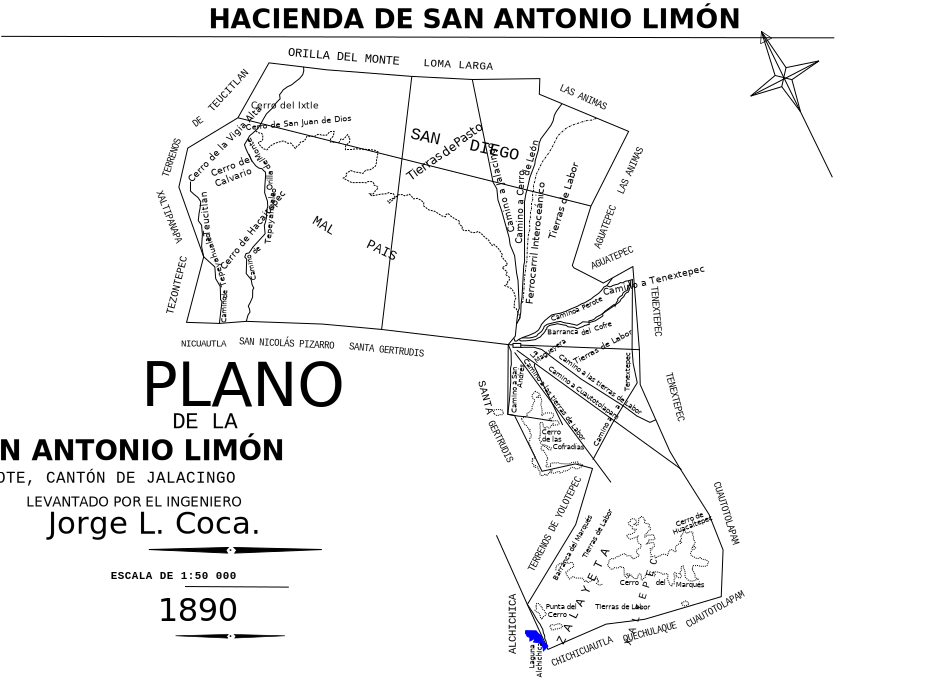
\includegraphics[height=13.1cm]{limon} % <--- limon by default
\caption[Plano de la hacienda de San Antonio Limón]{\index[lugares]{San Antonio Limon@San Antonio Limón!Plano@\textit{Plano}}\textsc{Fuente:} Luc Cambrezy y Bernal Lascurain, \emph{De la hacienda al ejido. Crónicas de un territorio fraccionado (Centro de Veracruz).} \textsc{larousse/orstom}/Centro de Estudios Mexicanos y Centroamericanos, México, 1992, p. 48.}
\label{fig:hda-limon}
\end{sidewaysfigure}

La hacienda de Cuautotolapam\index[lugares]{Cuautotolapam!hacienda} fue adquirida en condiciones similares. En 1870 José Antonio prestó a Francisco Hernández,\index[nombres]{Hernandez, Francisco@Hernández, Francisco} vecino de San Andrés Chalchicomula\index[lugares]{Chalchicomula} ---hoy Ciudad Serdán,\index[lugares]{Ciudad Serdán|see{Chalchicomula}} Puebla---\index[lugares]{Puebla} una cantidad de \$\,30000 con una tasa de intereses del 6 \% pagaderos a tres años, para comprar la hacienda.\footnote{\textsc{arppj}, 1873, Sec. 1"a, Inst. 4, fs. 4--6.} Imposibilitado para liquidar sus adeudos, Villegas concedió a Hernández un año de prórroga. Pero éste no pudo pagar y el 27 de enero de 1874 ambos decidieron dar por terminado el contrato.\footnote{\textsc{arppj}, 1873, Sec. 1"a, Inst. 74, fs. 91--93.} Agobiado por la deuda, Hernández se vio obligado a vender al año siguiente la propiedad en \$\,40000.\footnote{\textsc{arppj}, 1875, Sec. 1"a, Inst. 82, fs. 61--62.}
\begin{sidewaysfigure}
\centering
\includegraphics[height=13.8cm]{cuautotolapam}
\caption[Plano de la hacienda de Cuautotolapam]{\textsc{Fuente:} Cambrezy y Lascurain, \emph{op. cit.,} p. 50.\index[lugares]{Cuautotolapam!Plano@\textit{Plano}}}
\label{fig:hda-cuatotolapam}
\end{sidewaysfigure}

La hacienda de Tenextepec fue adquirida casi en las mismas condiciones que la de San Antonio Limón. En 1881, José Antonio Villegas compró el préstamo hipotecario ---capitales e intereses--- que Leonardo M. Rugama\index[nombres]{Rugama, Leonardo} había contraído con Joaquín\index[nombres]{Perez Larrea, Joaquin@Pérez Larrea, Joaquín} y Luis Pérez Larrea,\index[nombres]{Perez Larrea, Luis@Pérez Larrea, Luis} propietarios de la hacienda de San José de los Molinos,\index[lugares]{San Jose de los Molinos@San José de los Molinos!hacienda} por un monto de \$\,44563.\footnote{\textsc{arppj}, 1881, Sec. 1"a, Inst. 76, fs. 57--62. \textsc{arppj}, 1882, Sec. 1"a, Inst. 83, fs. 41--42.} Tenextepec\index[lugares]{Tenextepec!hacienda} tenía ya un largo camino recorrido en lo que se refería a imposiciones hipotecarias. Desde 1861 Leonardo M. Rugama\index[nombres]{Rugama, Leonardo} y su esposa Paula Rugama,\index[nombres]{Rugama, Paula} venían hipotecando la propiedad, transfiriendo el préstamo de mano en mano y teniendo dificultades en el pago del capital original pero no en los réditos.\footnote{\emph{Ídem}. \textsc{arppj}, 1875, Sec. 1"a, Inst. 89, fs. 65--66. \textsc{arppj}, 1875, Sec. 1"a, Inst. 90, fs. 66--67. \textsc{arppj}, 1875, Sec. 1"a, Inst. 91, f. 67.}
\begin{sidewaysfigure}
\centering
\includegraphics[height=13.8cm]{tenextepec}
\caption[Plano de la hacienda de Tenextepec]{\textsc{Fuente:} Cambrezy y Lascurain, \emph{op. cit.,} p. 92.\index[lugares]{Tenextepec!Plano@\textit{Plano}}}
\label{fig:hda-tenextepec}
\end{sidewaysfigure}

Los Rugama\index[nombres]{Rugama!familia} habrían de hipotecar Tenextepec por última vez a los Villegas.\index[nombres]{Villegas!familia} El 8 de julio de 1869 Leonardo hipotecó la propiedad a José María Bello,\index[nombres]{Bello, Jose Maria@Bello, José María} un próspero comerciante altotongués por una cifra de \$\,5093, con una tasa de interés del 12 \% anual pagaderos a tres años. Rugama no pudo liquidar su adeudo a los herederos de Bello,\index[nombres]{Bello, Jose Maria@Bello, José María!herederos} y éstos lo vendieron a José María Villegas del Campo\index[nombres]{Villegas del Campo, Jose Maria@Villegas del Campo, José María} ---medio hermano de José Antonio---\index[nombres]{Villegas Contreras, Jose Antonio@Villegas Contreras, José Antonio} por la cantidad de \$\,1200.\footnote{\textsc{arppj}, 1882, Sec. 1"a, Inst. 75, f. 35. El 25 de febrero de 1883, Rugama finiquitó su adeudo ---\$\,1436.85--- con Villegas del Campo. Al respecto véase \textsc{agnep}, Teziutlán, 1883, Inst. 18, fs. 27--28.} El 8 de agosto de 1883, José Antonio Villegas llevó ante la justicia al propietario e hijos solicitando el pago del préstamo\footnote{\textsc{arppj}, 1883, Sec. 1"a, Inst. 87, f. 76.} y ese mismo año perdieron la propiedad.\footnote{\textsc{arppj}, 1883, Sec. 1"a, Inst. 135, fs. 114--118. El precio de la hacienda se había cotizado en \$\,29000 y no lograba cubrir los \$\,48132 que Rugama debía a José Antonio. En la cláusula cuarta del contrato se especificó que «el excedente [debía ser] pagado en plazos en términos que convengan al acreedor y los sres. Rugama».} Rugama no cruzó los brazos como lo hicieron Limón\index[nombres]{Limon, Claudio Antonio@Limón, Claudio Antonio} y Hernández\index[nombres]{Hernandez, Francisco@Hernández, Francisco} respecto a sus haciendas. El 29 de mayo de 1889 volvería a comprar a José Antonio la hacienda por un valor de \$\,30000.\footnote{\textsc{arppj}, 1889, Sec. 1"a, Inst. 52, fs. 55--56.} Y es que la propiedad era demasiado valiosa para la familia;\index[nombres]{Rugama!familia} no sólo se venía heredando de padres a hijos, sino que constituía una de las unidades productivas más ricas en todo el valle de Perote:\index[lugares]{Perote!valle} comprendía una de las mayores extensiones en pinos, y su cercanía con el sistema de comunicaciones Golfo-Altiplano Central\index[lugares]{Mexico@México!golfo de} le agregaba un valor considerable.

Los Villegas habrían de sumar a través de las adjudicaciones hipotecarias dos haciendas más. El 20 de octubre de 1885, José Antonio se adjudicó la hacienda de Cerro de León,\index[lugares]{Cerro de Leon@Cerro de León!hacienda} propiedad de Francisco Calderón\index[nombres]{Calderon, Francisco@Calderón, Francisco} por un valor de \$\,14360.\footnote{\textsc{arppj}, 1885, Sec. 1"a, Inst. 187, fs. 143--144 y \textsc{arppj}, 1885, Sec. 1"a, Inst. 188, fs. 144--145.} El valor de la propiedad resultó insuficiente para cubrir el pago que la testamentaria\index[nombres]{Calderon, Francisco@Calderón, Francisco!testamentaria} tenía con José Antonio,\index[nombres]{Villegas Contreras, Jose Antonio@Villegas Contreras, José Antonio} pues en la escritura de venta aún salía debiendo \$\,5660.\footnote{\em Ídem.} La última hacienda que adquirieron los Villegas\index[nombres]{Villegas!familia} fue la de Santa Cruz.\index[lugares]{Santa Cruz!hacienda} El artífice de la adquisición fue José María~Villegas del Campo,\index[nombres]{Villegas del Campo, Jose Maria@Villegas del Campo, José María} medio hermano de José Antonio que entre los años 1888 y 1894 prestó al matrimonio Ríos Guzmán,\index[nombres]{Rios Guzman@Ríos Guzmán!matrimonio} propietarios de la hacienda, una cantidad de \$\,16000.\footnote{\textsc{arppj}, 1888, Sec. 1"a, Inst. 134, f. 147. \textsc{arppj}, 1889, Sec. 1"a, Inst. 38, fs. 41--43 y \textsc{arppj}, 1894, Sec. 1"a, Inst.~140, fs. 200--203.} Endeudados con Villegas, la familia Ríos Guzmán\index[nombres]{Rios Guzman@Ríos Guzmán!familia} se vio obligada a ceder la hacienda por un valor de \$\,40613,\footnote{\textsc{arppj}, 1905, Sec. 1"a, Inst. 105, fs. 647--658.} obteniendo del propietario que se las dejara en arrendamiento.

Los ranchos habrían de venir a engrosar el número de propiedades que la familia Villegas venía adquiriendo también a través de los préstamos hipotecarios. En 1882, José Antonio prestó a Miguel Valdés\index[nombres]{Valdes, Miguel@Valdés, Miguel} la cantidad de \$\,4000 con un interés anual del 12 \% pagaderos a tres años sobre el rancho «San Pedro Buenavista».\index[lugares]{San Pedro Buenavista!rancho}\footnote{\textsc{agnep}, Teziutlán, 1882, Inst. 52, fs. 82--85.} Un año más tarde, Valdés impondría un nuevo gravamen por una cifra de \$\,1034.\footnote{\textsc{arppj}, 1883, Sec. 1"a, Inst. 147, fs. 128--131.} Esta propiedad había sido adquirida con base en las leyes de terrenos baldíos decretada entre los años 1882 y 1886, y poseía una extensión de 583 ha, en una zona bastante fértil, con abundante agua y propicia para el cultivo del tabaco y la engorda de ganado mayor.\footnote{\emph{Ídem}. Los intereses de Villegas respecto a la comercialización y engorda de ganado mayor se hicieron patentes en esta escritura. En la octava cláusula de este contrato se señaló que «El sr. Valdés declara y confiesa, que son de la exclusiva propiedad del sr. Villegas, y tiene recibidos de este sólo para su engorda en su expresado rancho de Buena Vista, 200 novillos marcados con el fierro \textsc{av}».} A casi una década de la primera imposición hipotecaria, los herederos de Miguel Valdés\index[nombres]{Valdes, Miguel@Valdés, Miguel!herederos} adeudaban a José Antonio Villegas un monto de \$\,9683 ---capitales y réditos--- por lo que carentes de recursos, decidieron venderla por un valor total de \$\,12000.\footnote{\textsc{arppj}, 1891 (Libro 2), Sec. 1"a, Inst. 214, fs. 41--44.} Cinco años más tarde, José Antonio Villegas habría de apretar a través del oneroso mecanismo de los préstamos hipotecarios a Enrique Marín.\index[nombres]{Marin, Enrique@Marín, Enrique} En 1896 se apropió de su finca «Arroyo Zarco»\index[lugares]{Arroyo Zarco!rancho} por la cantidad de \$\,8000.\footnote{\textsc{arppj}, 1896, Sec. 1"a, Inst. 253, fs. 310--312.}
\begin{sidewaystable}
\scriptsize
\centering
\caption[Ranchos de la familia Villegas]{Ranchos de la familia Villegas.\index[nombres]{Villegas!ranchos (\emph{cuadro})}}
\begin{tabular}{@{}llllrr@{}}
\toprule
Comprador & Vendedor & Predio & Ubicación & Precio (\$) & Superficie (ha) \\
\midrule
J. A. Rivera Franquis\index[nombres]{Rivera Franquis, Jose Antonio@Rivera Franquis, José Antonio} y Ana Villegas\index[nombres]{Villegas, Ana} & {} & Olopiota,\index[lugares]{Olopiota} Checheloapan,\index[lugares]{Checheloapan} Cochota\index[lugares]{Cochota} y Napoala\index[lugares]{Napoala} & Atzalan\index[lugares]{Atzalan} y Jalacingo\index[lugares]{Jalacingo} & \texttlf{1734} & {} \\
Ana Villegas y J. A. Rivera Franquis & {} & Ixtahuanticpan\index[lugares]{Ixtahuanticpan} & {} & \texttlf{1600} & 2 caballerías \\
J. M. Villegas Contreras\index[nombres]{Villegas del Campo, Jose Maria@Villegas del Campo, José María} & Rafael Barreda\index[nombres]{Barreda, Rafaela} & La Peña\index[lugares]{Pena, La@Peña, La!predio} & Atzalan & \texttlf{3400} & {} \\
J. A. Villegas Contreras\index[nombres]{Villegas Contreras, Jose Antonio@Villegas Contreras, José Antonio} & Miguel Valdés\index[nombres]{Valdes, Miguel@Valdés, Miguel!herederos} Herederos & San Pedro Buenavista\index[lugares]{San Pedro Buenavista!rancho} & Atzalan & \texttlf{12000} & \texttlf{5817} \\
Leonardo Villegas\index[nombres]{Villegas Perdomo, Leonardo} & J. M. Villegas Contreras & La Peña & Atzalan & \texttlf{3000} & {} \\
J. A. Villegas Contreras & Enrique Marín\index[nombres]{Marin, Enrique@Marín, Enrique} & Arroyo Zarco\index[lugares]{Arroyo Zarco!rancho} & Buenavista\index[lugares]{San Pedro Buenavista} (Atzalan) & \texttlf{8000} & \texttlf{2000} \\
Quirino Villegas\index[nombres]{Villegas, Quirino} & R. Agüeros\index[nombres]{Agueros, Ruperto@Agüeros, Ruperto} y V. Calderón\index[nombres]{Calderon, Virginia@Calderón, Virginia} & Paxta\index[lugares]{Paxta} & Hueytamalco\index[lugares]{Hueytamalco} (Pue.)\index[lugares]{Puebla} & \texttlf{10000} & {} \\
Quirino Villegas & Marcelino Pumarino\index[nombres]{Pumarino, Marcelino} & La Peña\index[lugares]{Pena, La@Peña, La!rancho} & Nautla\index[lugares]{Nautla} (Misantla)\index[lugares]{Misantla} & \texttlf{16000} & \texttlf{334} \\
María Antonio Moya\index[nombres]{Antonio Moya, Maria@Antonio Moya, María} & J. M. Villegas Contreras & Tenextezala\index[lugares]{Tenextezala} & El Arco\index[lugares]{Arco, El} (Jalacingo)\index[lugares]{Jalacingo} & \texttlf{2920} & {} \\
Quirino Villegas & Fam. Santiesteban\index[nombres]{Santiesteban!familia} & Tlacuilolopan\index[lugares]{Tlacuilolopan|see{Atetehuetzin}} o Atetehuetzin\index[lugares]{Atetehuetzin} & Hueytamalco (Pue.) & \texttlf{5500} & \texttlf{615} \\
J. M. Villegas Campo & Roberto Burkle\index[nombres]{Burkle, Roberto} & Estugarda\index[lugares]{Estugarda} y Ojo de Agua\index[lugares]{Ojo de Agua} & Atzalan\index[lugares]{Atzalan} & \texttlf{2287} & \texttlf{275} \\
\bottomrule
\end{tabular}
\caption*{\textsc{Fuente:} \textsc{agnep} 1876--1910; \textsc{arppj}, 1872--1910.}
\label{tab:ranchos-villegas}
\end{sidewaystable}\protect\enlargethispage*{\baselineskip}

Las relaciones clientelares de la familia\index[nombres]{Villegas!familia} no sólo estaban circunscritas al valle de Perote\index[lugares]{Perote!valle} y los municipios que integraban el cantón de Jalacingo.\index[lugares]{Jalacingo!cantón} El prestigio de la familia, fincado en su enorme poder económico, era conocido más allá de las fronteras del entorno regional. En 1903, Quirino Villegas Contreras\index[nombres]{Villegas Contreras, Quirino} habría de apropiarse del rancho «La Peña»,\index[lugares]{Pena, La@Peña, La!rancho} propiedad de Marcelino Pumarino\index[nombres]{Pumarino, Marcelino} ubicado en Nautla,\index[lugares]{Nautla} cantón de Misantla,\index[lugares]{Misantla!cantón} por una cantidad de \$\,16000.\footnote{\textsc{arppj}, 1903, Sec. 4"a, fs. 10--14.} La adjudicación había acabado en muy malas relaciones entre ambos, pues Pumarino «ha destruido los techos de las casas de dicha finca para aprovecharse con perjuicio del acreedor, del producto de la venta de la lámina de Zinc que formaban dichos techos, [ésta] ha sufrido considerable demérito y consiguientemente una notable disminución en el precio de su valor».\footnote{\em Ídem.} La escritura revelaría con sorna que «El sr. Pumarino dijo: que no está conforme con el embargo practicado [y además] tiene otros acreedores a quien juzga de mejor derecho para aprovecharse del producto de la venta de las mercancías».\footnote{\em Ídem.} Como los \$\,16000 eran insuficientes para cubrir el pago del capital e intereses, Pumarino tuvo que otorgar a Villegas algunos~pagos extras, así como otros bienes raíces.

Meses antes de que iniciara la Revolución, José María Villegas del Campo\index[nombres]{Villegas del Campo, Jose Maria@Villegas del Campo, José María} se apropió de los predios rústicos «Estugarda\index[lugares]{Estugarda} y Ojo de Agua»,\index[lugares]{Ojo de Agua} propiedades de Roberto Burkle\index[nombres]{Burkle, Roberto} por un valor de \$\,2287 y con una extensión superficial de 245 ha en conjunto. Hipotecados desde 1897, su propietario no puso objeción alguna en la adjudicación.\footnote{\textsc{arppj}, 1909, Sec. 1"a, Inst. 41, fs. 90--94.}

Si de las ocho haciendas que llegaron a adquirir los Villegas, siete fueron obtenidas a través de adjudicaciones hipotecarias, el proceso de adquisición de los ranchos fue otro. Un análisis revela que cerca del 60 \% de los grandes ranchos fueron obtenidos a través de este mecanismo y un 40 \% ---pequeños~ranchos--- a través de la compra. Hay cierta lógica en este proceso. Los montos que la familia Villegas\index[nombres]{Villegas!familia} prestó a estos «rancheros» eran casi y sólo equiparables al de los hacendados. En efecto, se trataba de propiedades incluso más grandes y potencialmente más productivas que algunas haciendas del valle de Perote;\index[lugares]{Perote!valle} como en el caso de los ranchos «San Pedro Buenavista»\index[lugares]{San Pedro Buenavista!rancho} (5817 ha) y «Arroyo Zarco»\index[lugares]{Arroyo Zarco!rancho} (2800 ha).\footnote{Estos ranchos eran superficialmente más grandes que las haciendas Ximonco\index[lugares]{Ximonco!hacienda} y Santa Ana.\index[lugares]{Santa Ana!hacienda} La primera poseía una extensión apenas de un millar de hectáreas, y la segunda una superficie de 4200 ha. La dificultad por diferenciar y definir el rancho de la hacienda ha sido tema de controvertidos debates. Isabel Gil Sánchez\index[nombres]{Gil Sanchez, Isabel@Gil Sánchez, Isabel} y Marco Bellingeri\index[nombres]{Bellingeri, Marco} han sostenido el carácter insuficiente que la extensión superficial desempeña en la definición de rancho y hacienda. Para ellos, hacienda es «una unidad de producción agrícola con posesión privada sobre la tierra, fundamentalmente mercantil, aun si su producción se basa en la articulación del autoconsumo y de una verdadera producción para el mercado». Pienso que esta definición también es insuficiente, pues los mismos criterios pueden ser aplicados al rancho. Para estos autores, rancho es «una unidad productiva dependiente o independiente de la hacienda ---según si está o no arrendada--- de dimensiones variables, pero generalmente inferiores a las de aquellas, que se caracteriza por no contar con peones acasillados y que dispone del trabajo de la totalidad de los miembros de la familia del propietario o arrendatario, y de trabajo eventual estacional». Esta definición también adolece de imprecisiones. Estamos de acuerdo en los peones acasillados, en la dependencia o independencia que éste [el rancho] pueda tener respecto a la hacienda y en el trabajo eventual estacional; pero no en sus dimensiones, ni en la fuerza de trabajo de los miembros de la familia o arrendatario. Los ranchos San Pedro Buenavista y Arroyo Zarco eran mucho más grandes que algunas haciendas del llano perotense\index[lugares]{Perote!haciendas} y existía siempre la posibilidad de contratar mano de obra para trabajar el rancho ---independientemente si son familiares o no. Al respecto, véase Marco Bellingeri e Isabel Gil Sánchez, «Las estructuras agrarias» en Cardoso, \emph{op. cit.,} pp. 98--100.}

Es importante mencionar la dificultad que tenían rancheros y hacendados para cubrir sus pagos con la familia. Tan importante es, que cuatro de las ocho haciendas ubicadas en el llano\index[lugares]{Perote!llano} y el 60 \% de los ranchos fueron adquiridos por ésta precisamente, por falta de pago. ¿Es acaso qué no eran lo suficientemente productivas? ¿Qué sentido tendría para los Villegas invertir sus capitales en propiedades con estas características? Si lo eran ¿por qué~sus propietarios no pudieron salir adelante con sus deudas? ¿Prefirieron perderlas y drenar e invertir el dinero obtenido en préstamo en negocios más rentables? ¿Será que heladas y sequías en este periodo provocaron y descapitalizaron a estos propietarios?

Poseer demasiada tierra no implicaba necesariamente que ésta fuera totalmente productiva; es decir, se podía tener un millón de hectáreas y sólo destinar para su cultivo 50 ha o 100 ha de las mismas. Aunque el resto permanecía sin producir ganancias, no dejaba de ser una propiedad que representaba un capital, aunque estuviera amortizado. Existía la posibilidad de arrendarla, subarrendarla; de establecer contratos con los `medieros' para maximizar las ganancias; de fraccionar y vender los predios menos productivos para recuperar parte del capital. El mapa elaborado por Luc Cambrezy\index[nombres]{Cambrezy, Luc} y Bernal Lascurain\index[nombres]{Lascurain, Bernal} sobre la hacienda de Cuautotolapam\index[lugares]{Cuautotolapam!hacienda} (\emph{v.} Imagen \ref{fig:hda-cuatotolapam}, pág. \pageref{fig:hda-cuatotolapam}) revela que ésta explotaba de facto 3874-48-01 ha de tierra de temporal, disponiendo potencialmente para su explotación cerca de 3535-56-92 ha de montes.\footnote{Cambrezy y Lascurain, \emph{op. cit.,} p. 50.} Es decir, que de las 10059 ha que poseía la hacienda, sólo el 73.66 \% eran susceptibles de cultivo. No obstante, este número de hectáreas se reduce ya que en las estadísticas de Southworth\index[nombres]{Southworth, John R.} y Falcón\index[nombres]{Falcon, Romana@Falcón, Romana} y García Morales,\index[nombres]{Garcia Morales, Soledad@García Morales, Soledad}\footnote{Southworth, \emph{op. cit.,} p. 244. Falcón y García, \emph{op. cit.,} pp. 36--37.} la Cuautotolapam manifestó tan sólo dedicarse al cultivo de cereales como el trigo, maíz, cebada y haba, así como a la extracción de raíz de zacatón y pulque; al no hablar de explotación maderera se deduce que las 3535 ha de montes no estaban siendo explotadas, o que esta información se omitió. Si nos dejamos guiar por las cifras, encontramos que sólo el 38.51 \% de las tierras de la hacienda eran productivas.

Aunque no disponemos del número de hectáreas que las haciendas Ximonco,\index[lugares]{Ximonco!hacienda} Tenextepec,\index[lugares]{Tenextepec!hacienda} San Antonio\index[lugares]{San Antonio Limon@San Antonio Limón!hacienda} y Cerro de León\index[lugares]{Cerro de Leon@Cerro de León!hacienda} destinaban para el cultivo, hay evidencias de que sí eran lo suficientemente productivas. Como ha señalado Abel Juárez,\index[nombres]{Juarez Martinez, Abel@Juárez Martínez, Abel} hacia 1890 las haciendas, ranchos y congregaciones del valle cultivaban 30000 ha de temporal; 6000 ha de riego, 14000 ha con pastizales para ganado mayor y menor, y disponían de 20010 ha para la extracción de madera.\footnote{Abel Juárez Martínez, «El trabajo en la hacienda de San José de los Molinos, en Veracruz (\mbox{1890--1910})» en Mario Cerutti (Coord.), \emph{De los Borbones a la Revolución. Ocho estudios regionales.} \textsc{comecso/gv} Editores/Universidad Autónoma de Nuevo León, 1986, pp. 186--187.} Esto quiere decir que de las 69930 ha que poseían las haciendas, poco más del 100 \% eran explotadas. No es fortuito que para esas fechas Miguel S. Perdomo,\index[nombres]{Perdomo, Miguel S.!jefe político} jefe político de Jalacingo,\index[lugares]{Jalacingo!jefe político} sostuviera ante la legislatura\index[lugares]{Veracruz!Congreso} del estado que el cantón\index[lugares]{Jalacingo!cantón} experimentaba un crecimiento paulatino de las actividades agrícolas. Afirmó que en las tierras frías, pese a las funestas consecuencias que dejó el ciclón de 1888, los agricultores habían logrado producir cantidades considerables de cereales y leguminosas; en la zona templada, que comprendía las municipalidades de Altotonga,\index[lugares]{Altotonga!municipio} Jalacingo\index[lugares]{Jalacingo!municipio} y Atzalan,\index[lugares]{Atzalan!municipio} los campesinos habían incrementado su producción de maíz, frijol y cebada; y finalmente en la tierra caliente, que abarcaba porciones de Atzalan,\index[lugares]{Atzalan} Tlapacoyan\index[lugares]{Tlapacoyan} y Martínez de la Torre,\index[lugares]{Martinez de la Torre@Martínez de la Torre} productos para la exportación como el café y el tabaco, así como la cría y engorda de ganado mayor, habían experimentado un auge considerable.\footnote{Soledad García Morales, \emph{Jefes políticos y regiones veracruzanas, 1880--1900.} Universidad Nacional Autónoma de México, México, 2000, p. 161 [Tesis doctoral].}

Las actividades agrícolas del valle\index[lugares]{Perote!valle} estaban mucho más diversificadas e iban más allá de la simple producción de cereales. La hacienda de San José de los Molinos,\index[lugares]{San Jose de los Molinos@San José de los Molinos!hacienda} además de dedicarse a las actividades agropecuarias, era la única propiedad que poseía una fábrica de hilados y tejidos: \emph{La Claudina.} Movilizada por fuerza hidráulica, la factoría pertenecía a un conjunto más amplio de establecimientos textiles e intereses en poder de unos hermanos españoles de apellidos Mier y Rubín,\index[nombres]{Mier y Rubin@Mier y Rubín!hermanos} que se extendían hasta la ciudad de Puebla.\index[lugares]{Puebla!ciudad}

La hacienda de Tenextepec\index[lugares]{Tenextepec!hacienda} y sus propietarios los Rugama,\index[nombres]{Rugama!familia} habían volcado sus capitales e intereses en la explotación de los ricos bosques del cofre de Perote.\index[lugares]{Perote!cofre de} Tan fuertes eran, que la familia hizo construir de manera particular una línea férrea entre la hacienda y el bosque que entroncaba con el Ferrocarril Interoceánico para su extracción. En efecto, la riqueza maderera del cofre venía siendo explotada indiscriminadamente por toda una caterva de hacendados y rancheros, que venían colocando el producto en sitios como Xalapa,\index[lugares]{Xalapa} Veracruz (Puerto),\index[lugares]{Veracruz!puerto} Alvarado\index[lugares]{Alvarado} y Tlacotalpan\index[lugares]{Tlacotalpan} en el estado de Veracruz,\index[lugares]{Veracruz!estado} y Atlixco,\index[lugares]{Atlixco} Puebla\index[lugares]{Puebla} y la ciudad de México\index[lugares]{Mexico@México!ciudad} en el Altiplano Central.\footnote{Abel Juárez Martínez, «Crónica de un ecocidio: el llano de Perote» en \textit{Anuario \textsc{vii}.} Centro de Investigaciones Históricas de la Universidad Veracruzana, Xalapa, 1990, pp. 71--72. Roberto Vélez Pliego,\index[nombres]{Velez Pliego, Roberto@Vélez Pliego, Roberto} exdirector del Instituto de Ciencias Sociales y Humanidades (\textsc{buap}) me dijo que, cuando se inició la remodelación del Hotel Arronte\index[nombres]{Arronte!Hotel@\textit{Hotel}} (av. Juan de Palafox y Mendoza,\index[nombres]{Palafox y Mendoza, Juan de} núm. 219, Puebla, Pue.)\index[lugares]{Puebla!ciudad} en la década de los noventa (s. \textsc{xx}), los trabajadores retiraron una gran cantidad de vigas y polines \emph{apolillados}, procedentes de la hacienda de Tenextepec. «Muchas [vigas y polines] venían grabadas con la marca de fuego: Cruz Rugama y C\textsu{ia},\index[nombres]{Cruz Rugama!compañía} Hda. de Tenextepec, Perote, Ver».\index[lugares]{Perote} Roberto Vélez Pliego, comunicación personal, julio del 2007.} Esta asesina e inconsciente tala inmoderada trajo severas consecuencias para el valle.
\begin{quoting}
al empezar los desmontes, recuerda un informante, se sucedió la escasez de lluvias y los maizales murieron, los campos no se volvieron a poblar de plantas altas y de tronco macizo con mazorcas frondosas: en su lugar aparecieron milpillas raquíticas amarillentas que poseían en su seno un
`molcate' en lugar de mazorca; del trigo ya ni hablar, desde entonces desapareció el valle.\footnote{Abel Juárez Martínez, «Los rancheros. Un nuevo grupo en el poder (1910--1920)» en Mirna Benítez; Carmen Blázquez Domínguez \emph{et al., Veracruz, un tiempo para contar. Memoria del 1"er Seminario de Historia Regional.} Universidad Veracruzana/Instituto Nacional de Antropología e Historia, México, 1989, pp. 184--185 [Regiones de México].}
\end{quoting}
De este modo, los latifundistas del valle\index[lugares]{Perote!valle} sacaron el máximo usufructo de sus propiedades sin importarles los riesgos. Además del lucrativo negocio de la madera, las haciendas habían destinado parte de sus tierras para la cría y engorda de ganado mayor y menor. Las dimensiones de los corrales de las haciendas, que en ocasiones abarcaban varias hectáreas, revelan la importancia que ésta desempeñaba dentro de las actividades económicas del valle.\footnote{Cambrezy y Lascurain, \emph{op. cit.,} pp. 22--24.} De este modo lograron producir carne, cueros, leche y todos sus derivados; además de dedicarse a la porcicultura y la ganadería de pastoreo.\footnote{\emph{Ibid.,} p. 83.} La comercialización de todos estos productos se reducía a satisfacer las necesidades de un mercado local y regional.

En el caso de los ranchos es más difícil poder determinar el número de hectáreas que éstos destinaban para su producción, ya que las fuentes consultadas son bastante estériles en este aspecto. Sin embargo, podemos inferir por su ubicación geográfica y los escasos datos encontrados en el~\textsc{arppj}, que se trataba de propiedades aptas para la ganadería mayor y el cultivo de productos tropicales como el café, el tabaco, la caña de azúcar y los cítricos, con una amplia demanda en los mercados local, regional e internacional. Al comprar el rancho «La Peña»\index[lugares]{Pena, La@Peña, La!rancho} en 1891, José María Villegas Contreras\index[nombres]{Villegas del Campo, Jose Maria@Villegas del Campo, José María} también había adquirido «70 cabezas de ganado vacuno de un año arriba del criadero que en dicho rancho tiene, las cuales están marcadas con el fierro del vendedor, cuyo fierro tiene cedido al comprador para que continúe usándolo como suyo».\footnote{\textsc{arppj}, 1891, Sec. 1"a, Inst. 93, fs. 129--130.}

Las potencialidades agrícolas del rancho «San Pedro Buenavista»\index[lugares]{San Pedro Buenavista!rancho} se hicieron notables en 1891. En la escritura de adjudicación se mencionó que «el referido rancho está dividido en potreros con pasto natural y una extensión de 60 estajos [42.12 ha] de zacate del Pará\index[lugares]{Africa@África!Pará} [\emph{Brachiaria mutica}] en mal estado y lo demás en Monte Alto».\footnote{\textsc{arppj}, 1891, Sec. 1"a (Libro 2), Inst. 214, fs. 41--44. Corchetes míos.} En el litigio de 1903 entre Quirino Villegas Contreras\index[nombres]{Villegas Contreras, Quirino} y Marcelino Pumarino\index[nombres]{Pumarino, Marcelino} sobre el rancho «La Peña»,\index[lugares]{Pena, La@Peña, La!rancho} se mencionó que dicha propiedad poseía «arrendamiento de pastos que el sr. Pedro Naude\index[nombres]{Naude, Pedro} debe pagar al sr. Pumarino, por razón de los ganados [...] y se encuentran pastando en la mencionada finca [...]. Las mercancías, aparadores, caja de fierro, mesas de juego, prensa de copiar y escritorio existentes en la tienda».\footnote{\textsc{arppj}, 1903, Sec. 4"a, fs. 10--14.} Es importante mencionar que de los once ranchos que la familia\index[nombres]{Villegas!familia} llego a poseer, ocho de ellos se ubicaban en la tierra caliente.

Ahora bien, revelar los efectos económicos y sociales que las sequías de 1875, 1884, 1886 y 1894 tuvieron sobre el valle de Perote\index[lugares]{Perote!valle} y otras partes del cantón, aún está por determinarse. Sin embargo, es interesante hacer notar que este periodo de sequías coincide con las adjudicaciones que hizo la familia Villegas de sus haciendas y ranchos. En efecto, en 1875 la familia obtuvo las haciendas de San Antonio\index[lugares]{San Antonio Limon@San Antonio Limón!hacienda} y Cuautotolapam;\index[lugares]{Cuautotolapam!hacienda} y en 1885, la de Cerro de León;\index[lugares]{Cerro de Leon@Cerro de León!hacienda} sólo el rancho «Arroyo Zarco»\index[lugares]{Arroyo Zarco!rancho} fue adquirido en 1896. Es decir, que de las cuatro haciendas que poseía la familia en esta área, la adquisición~de tres coincide con las sequías y los procesos de adjudicación. El valle de Perote, a pesar de ubicarse geopolíticamente en el estado de Veracruz,\index[lugares]{Veracruz!estado} histórica y geográficamente siempre se ha vinculado al Altiplano Central. El hecho de que las haciendas de esta área hayan practicado una agricultura fincada en el cultivo de cereales durante la centuria decimonona ---similar a las del valle Puebla-Tlaxcala---,\index[lugares]{Puebla-Tlaxcala!valle} confirma las similitudes que tenían con aquéllas.

El valle peroteño no estuvo exento de las calamidades climatológicas. Si bien el ciclón de 1888 había contraído la economía de la región, ésta había salido avante en los años siguientes. Dado que el valle\index[lugares]{Perote!valle} se sitúa y comprende parte de la meseta central ---la cual recibe sólo el 12 \% de lluvias de todo el territorio nacional---, no es casual que éste padeciera las consecuencias de las sequías. Enrique Florescano\index[nombres]{Florescano, Enrique} ha señalado que una baja ligera en el índice de lluvias en esta área, provocaba desequilibrios económicos de magnitudes nacionales, por la importancia que tenía en la producción de cereales.\footnote{Enrique Florescano, \emph{Breve historia de la sequía en México.} Consejo Nacional para la Cultura y las Artes, México, 2000, p. 39 [Regiones].}

El clima seco y la altura sobre el nivel el mar, fueron factores que favorecieron la producción de granos en esta área. El hecho de que la cebada y el trigo requieran de un mínimo de temperatura de 3\,°C y un máximo de 28\,°C y una temporalidad menor para su germinación y maduración muy superiores a los del maíz,\footnote{Este grano necesita un mínimo de temperatura de 8\,°C y un máximo de 44\,°C. Además, necesita de 80 a 140 días para su completa maduración.} hacía que los productores de esta área invirtieran sus capitales en cultivos más seguros. Esto es factible para todo el valle, pues como se podrá observar, el trigo y la cebada no sólo requieren de condiciones de humedad, temperatura y tiempo de maduración menores a los del maíz, sino que por otra parte, son más resistentes al granizo y heladas tan recurrentes de las zonas frías. Son quizá estas características las que influyeron entre los hacendados y rancheros, para invertir sus capitales de manera segura.

En el último tercio del siglo \textsc{xix}, se presentaron en todo el país cuatro grandes sequías. La de 1877 afectó principalmente el valle de México\index[lugares]{Mexico@México!valle} y se prolongó hasta el año siguiente; la de 1891 fue la peor de todas, pues no sólo se sintió con intensidad afectando a todo el país, sino que duró hasta 1892. En cuanto a sequías de carácter regional con impactos profundos, se tiene la de 1868, que azotó principalmente a Chiapas,\index[lugares]{Chiapas} Oaxaca,\index[lugares]{Oaxaca} Guerrero,\index[lugares]{Guerrero} Aguascalientes,\index[lugares]{Aguascalientes} Coahuila,\index[lugares]{Coahuila} el valle de México y Veracruz.\index[lugares]{Veracruz}\footnote{Florescano, \emph{op. cit.,} p. 48.} Florescano sostiene que las sequías más severas se presentaron a finales del siglo \textsc{xix} entre las que se incluyen las de 1877--1878 y 1891--1892.\footnote{\em Ídem.}

La falta de agua en el llano perotense\index[lugares]{Perote!llano} no sólo fue una amenaza constante para las cosechas de hacendados y rancheros, sino también el centro de sus preocupaciones. En 1878 José Antonio Villegas Contreras,\index[nombres]{Villegas Contreras, Jose Antonio@Villegas Contreras, José Antonio} propietario del Molino de Guadalupe,\index[lugares]{Molino de Guadalupe!hacienda} se vio obligado a comprar un predio pequeño y perder los intereses de un capital que le adeudaban Santiago Flores\index[nombres]{Flores, Santiago} y Manuel Ortiz Canelo\index[nombres]{Ortiz Canelo, Manuel} «porque han convenido en que Flores por esta cantidad rebajada de \$\,48.50 concede a Villegas que pueda éste pasar en canoas por el lugar que le convenga en los terrenos de Flores, el agua que necesite del río para que pueda [¿regar?] los terrenos de Villegas».\footnote{\textsc{arppj}, 1878, Sec. 1"a, Inst. 5, f. 8.}

Ese mismo año, José Antonio Villegas Contreras habría de llevar ante la justicia a Heliodoro Lozada\index[nombres]{Lozada, Heliodoro} y José Antonio Aguilar,\index[nombres]{Aguilar, Jose Antonio@Aguilar, José Antonio} administradores del Molino «La Reforma»\index[lugares]{Reforma, La!molino} y la hacienda de San José de los Molinos\index[lugares]{San Jose de los Molinos@San José de los Molinos!hacienda} respectivamente, por «retener la posesión y uso de aguas que con el nombre de Río de Sierra de Agua\index[lugares]{Sierra de Agua!río} baja de la montaña del Cofre de Perote\index[lugares]{Perote!cofre de} a dar movimiento al molino llamado de  `Guadalupe'\index[lugares]{Molino de Guadalupe!molino} situado en la Congregación de Cerro de León».\index[lugares]{Cerro de Leon@Cerro de León!congregación}\footnote{\textsc{arppj}, 1878, Sec. 1"a, Inst. 139, fs. 107--108.} La rivalidad entre estos hacendados era evidente, pues José Antonio Villegas había intentado días antes a la demanda, establecer un pacto conciliatorio, que éstos no aceptaron. En el proceso judicial ---efectuado el 27 de mayo de 1878--- se acordó que Lozada y Aguilar, una vez satisfechas sus necesidades del hidrante, dejarían correr el resto para beneficio de las congregaciones de Sierra de Agua\index[lugares]{Sierra de Agua!congregación} y Cerro de León, permitiendo a José Antonio Villegas hacer todas las construcciones necesarias en la propiedad de éstos para abastecerse del líquido.\footnote{\em Ídem.}

Este éxito que José Antonio logró adjudicarse contra Lozada y Aguilar, fue probablemente resultado de las estrechas relaciones políticas que mantuvo con el entonces jefe político, Manuel S. Castellanos,\index[nombres]{Castellanos, Manuel S.!jefe político} pero principalmente~con el entonces titular del Juzgado de Paz: Miguel María de Guzmán.\index[nombres]{Guzman, Miguel Maria de@Guzmán, Miguel María de} En efecto, José Antonio tenía parentesco político con los Guzmán.\index[nombres]{Guzman@Guzmán!familia} Su sobrina Carmen Villegas Guzmán,\index[nombres]{Villegas Guzman, Carmen@Villegas Guzmán, Carmen} hija de su medio hermano Miguel Villegas del Campo,\index[nombres]{Villegas del Campo, Miguel} había contraído nupcias con Miguel María de Guzmán (padre),\index[nombres]{Guzman, Miguel Maria de@Guzmán, Miguel María de!jefe político} quien llegó a ser jefe político del cantón en 1892,\footnote{No sabemos cuál de los dos llegó a ser jefe político; esto se debe a que en los registros del \textsc{arppj} el segundo apellido nunca apareció.} confirmándonos las relaciones políticas y de sangre ---por medio de su sobrina Carmen---\index[nombres]{Villegas Guzman, Carmen@Villegas Guzmán, Carmen} que éste mantenía con Guzmán.\index[nombres]{Guzman, Miguel Maria de@Guzmán, Miguel María de}

Pero los problemas por el uso del agua continuarían. Hay datos que confirman que las relaciones entre José Antonio Villegas\index[nombres]{Villegas Contreras, Jose Antonio@Villegas Contreras, José Antonio} y los hacendados del valle\index[lugares]{Perote!hacendados} eran bastante «tirantes». Todo indica que los dueños del molino «La Reforma»\index[lugares]{Reforma, La!molino} y la hacienda de San José de los Molinos,\index[lugares]{San Jose de los Molinos@San José de los Molinos!hacienda} a través de sus administradores y las autoridades del ayuntamiento de Perote,\index[lugares]{Perote!ayuntamiento} pusieron a José Antonio obstáculos para proveerse del líquido. Esto se observa en un contrato privado del 4 de agosto de 1887 que José Antonio Villegas y Rosendo Velázquez\index[nombres]{Velazquez, Rosendo@Velázquez, Rosendo} celebraron, en el que constaba que:
\begin{quoting}
convencido el último de la falta de derechos en el ayuntamiento de Perote para venderle una paja de agua de la fuente pública~de Cerro de León\index[lugares]{Cerro de Leon@Cerro de León} puesto que aquel Honorable cuerpo no salió a la evicción ha determinado desistir por completo del juicio procurando por medio de arreglos privados ulteriores controversias. Ambos de común acuerdo hemos tenido un convenio particular en virtud del cual el sr. Velázquez pueda continuar la obra hasta tomar de la primera fuente la cantidad de agua que necesite para mantener llena una pequeña fuente que ha construido en su casa y en la cantidad necesaria para el servicio doméstico y no más: \emph{queda a la vez facultado el sr. José Antonio Villegas para construir sobre el terreno de la propiedad del sr. Velázquez y de su representado un caño de cal y canto con el objeto de tomar en el punto más conveniente del costado del pilancón grande el derrame de éste y conducido al curso del agua que va hacia el molino de Guadalupe\index[lugares]{Molino de Guadalupe} con la construcción de ese caño no se impedirá ni estorbará el paso que tiene el sr. Velázquez establecido para llevar sus carretas a las trojes de su propiedad.}\footnote{\textsc{arppj}, 1887, Sec. 1"a, Inst. 93, fs. 64--65. Las cursivas son mías.}
\end{quoting}
Es muy probable que la mala relación entre José Antonio\index[nombres]{Villegas Contreras, Jose Antonio@Villegas Contreras, José Antonio} y sus adversarios, tuviera como trasfondo aspectos económicos. En el mundo de los negocios y los intereses agrícolas del valle,\index[lugares]{Perote!valle} poner obstáculos al contrario siempre traía ventajas económicas. La desgastada relación entre José Antonio Villegas y Joaquín Pérez Larrea\index[nombres]{Perez Larrea, Joaquin@Pérez Larrea, Joaquín} se confirma cuando en 1891, el primero celebró con Juan Mier y Rubín,\index[nombres]{Mier y Rubin, Juan@Mier y Rubín, Juan} ahora propietario de la hacienda de San José de los Molinos,\index[lugares]{San Jose de los Molinos@San José de los Molinos!hacienda}\footnote{La compró a Joaquín Pérez Larrea en 1890 por \$\,100000. En este sentido véase Abel Juárez Martínez, \emph{San José de los Molinos, Veracruz.} Secretaría de Educación y Cultura, Xalapa, 2005, p. 24.} un nuevo contrato por el uso de las aguas. En la escritura se señalaba que
\begin{quoting}
mas como posteriormente por el año de 1881 con arreglos celebrados en escritura pública don Joaquín Pérez Larrea y el Lic. don Manuel Villegas\index[nombres]{Villegas Contreras, Manuel!abogado} a nombre de su hermano don José Antonio, se hicieron algunas modificaciones a la transacción enunciada de 27 de mayo de 1878, \emph{dejando salvos los derechos que competen al exponente contra el vendedor don Joaquín Pérez por la diferencia entre la transacción referida y los arreglos hechos en la escritura mencionada, cuyos derechos hará valer contra el sr.~Pérez en su conformidad,} a cuyo fin los deja ilesos.\footnote{\textsc{arppj}, 1891, Sec. 1"a, Inst. 155, fs. 224--226. Las cursivas son nuestras.}
\end{quoting}
El uso del líquido indica que no estaba destinado para la irrigación de los cultivos ---salvo la compra que hizo José Antonio a Flores\index[nombres]{Flores, Santiago} y Ortiz Canelo\index[nombres]{Ortiz Canelo, Manuel} en 1878---, sino para la generación de fuerza hidráulica que movilizara los molinos. En las escrituras de 1878, 1887 y 1891, se menciona al menos la existencia de dos molinos (entre ellos Guadalupe\index[lugares]{Molino de Guadalupe!molino} y La Reforma),\index[lugares]{Reforma, La!molino} sin tomar en cuenta el uso que hiciera de las aguas la hacienda de San José de los Molinos,\index[lugares]{San Jose de los Molinos@San José de los Molinos!hacienda} pero se infiere que ésta probablemente también hacía lo mismo pues contaba con su propio molino.

Las sequías de este periodo debieron haber provocado desajustes en la economía del valle.\index[lugares]{Perote!valle} Dado que el 51.42 \% de las tierras de las haciendas fueron destinadas para el cultivo de los cereales, no es fortuito que éstos tuvieran una merma considerable. Cerca del 42.85 \% de las tierras de las haciendas y ranchos eran de temporal, lo que hacía que sólo se obtuviera una cosecha al año. Sólo el 8.57 \% de las tierras de estas propiedades eran de riego. La ganadería debió presentar dificultades similares, pues como señala Florescano\index[nombres]{Florescano, Enrique} el ganado vivió momentos críticos en 1875, 1884, 1886 y 1894.\footnote{Florescano, \emph{op. cit.,} p. 36.} Disponer de la cantidades producidas por cada una de las haciendas del valle en el periodo 1872--1910, ayudaría a clarificar notablemente el impacto de las sequías. Descubrir las razones de porqué hacendados y rancheros perdieron sus propiedades ante los Villegas,\index[nombres]{Villegas!familia} sigue siendo una tarea pendiente.
\section{El comercio}
\label{sec:el-comercio}
Es paradójico que en los registros consultados en el \textsc{arppj} y el \textsc{agnep} durante el periodo 1872--1910, encontremos el apellido de la familia muy vinculado al comercio, y a la vez no brinden la suficiente información sobre los productos que comercializaban, las cantidades que de ellos producían, dónde se comercializaban, qué mercados controlaban y cuáles eran sus ganancias. En cada operación que realizaron ante el \textsc{arppj} o el notario, el uso y el calificativo que ellos mismos se dieron como «comerciantes» fue muy frecuente. A diferencia de la familia Guzmán,\index[nombres]{Guzman@Guzmán!familia} cuyos miembros crearon casas de comercio de manera temprana, los Villegas incursionaron en forma tardía en este rubro. Tras el fallecimiento de José Antonio Villegas Contreras, sus hermanas y herederas universales ---Rosa, Guadalupe y Ana María Villegas del Campo---, crearon a principios del siglo \textsc{xx} la Sociedad «José Antonio Villegas Sucesores»,\index[nombres]{Villegas Contreras, Jose Antonio@Villegas Contreras, José Antonio!sucesores} una negociación que además de perpetuar el nombre del creador de la riqueza familiar, tenía por objetivo explotar los productos de tres de las ocho haciendas que llegaron a poseer: San Antonio Limón\index[lugares]{San Antonio Limon@San Antonio Limón!hacienda} y Cuautotolapam\index[lugares]{Cuautotolapam!hacienda} en el valle de Perote,\index[lugares]{Perote!valle} y Techachalco\index[lugares]{Techachalco} en el estado de Puebla.\index[lugares]{Puebla!estado}

A principios del siglo \textsc{xx}, Luis\index[nombres]{Villegas, Luis} y Gabriel Villegas,\index[nombres]{Villegas, Gabriel} miembros de la tercera generación, crearon una sociedad mercantil que tuvo por objeto tomar en arrendamiento la hacienda de «El Rincón»,\index[lugares]{San Miguel del Rincon@San Miguel del Rincón!hacienda} propiedad de Ana María Villegas del Campo\index[nombres]{Villegas del Campo, Ana Maria@Villegas del Campo, Ana María} y explotar todos sus ramos agrícolas.\footnote{\textsc{agnep}, Teziutlán, 1908, Prot. \textsc{ii} Sem., Inst. 62, fs. 209--213.} Dos años más tarde, sus primos Ángel\index[nombres]{Villegas Bello, Angel@Villegas Bello, Ángel} y Rafael Villegas\index[nombres]{Villegas Bello, Rafael} hicieron lo mismo con el propósito de «la compra y venta de abarrotes y ropa al por mayor y al menudeo».\footnote{\textsc{arppj}, 1884, Sociedades y poderes, Inst. 129, fs. 129--131.} Es decir, que sólo disponemos de la información sobre los intereses comerciales de una parte de la familia, pero no de la primera y segunda generación.

Sin embargo, no es aventurado pensar que las primeras dos generaciones de la familia\index[nombres]{Villegas!familia} canalizaran sus capitales e intereses comerciales a partir del complejo de haciendas del valle de Perote.\index[lugares]{Perote!haciendas} El hecho de que José Antonio Villegas\index[nombres]{Villegas Contreras, Jose Antonio@Villegas Contreras, José Antonio} y sus hermanos concentraran parte de sus capitales en esta área, llegando a poseer cuatro de las ocho haciendas existentes, nos habla de las pretensiones que tenían en la zona. Al detentar poco más del 47.40 \% de la tierra privada del valle, la familia no sólo reafirmaba su calidad latifundista, sino que marcaba la pauta en cuanto a la producción y comercialización de los productos en el área. En efecto, las haciendas de Ximonco,\index[lugares]{Ximonco!hacienda} San Antonio Limón,\index[lugares]{San Antonio Limon@San Antonio Limón!hacienda} Cuautotolapam\index[lugares]{Cuautotolapam!hacienda} y Cerro de León,\index[lugares]{Cerro de Leon@Cerro de León!hacienda} eran conocidas por su producción de cereales, la explotación de sus maderas, la engorda de ganado mayor y menor, y la producción de pulque.

En este sentido, los granos ocupaban un lugar importante en los intereses comerciales de la familia. En 1874, José María\index[nombres]{Villegas del Campo, Jose Maria@Villegas del Campo, José María} y Quirino Villegas Contreras,\index[nombres]{Villegas Contreras, Quirino} propietarios de la hacienda de San Juan Ximonco, la arrendaron a José María Fernández\index[nombres]{Fernandez, Jose Maria@Fernández, José María} señalándose que
\begin{quoting}
El mismo arrendamiento que hacen los cc. Villegas al c. Fernández de la finca referida, \emph{es con la previa condición de que el~trigo que produzcan las cosechas de la referida finca durante el tiempo del arrendamiento, lo dará en venta a los locadores} en los meses de enero de cada uno de esos [siete] años al precio que lo pague en Perote,\index[lugares]{Perote} el sr. Joaquín Pérez Larrea\index[nombres]{Perez Larrea, Joaquin@Pérez Larrea, Joaquín} a su representante para su molino de agua.\footnote{\textsc{arppj}, 1874, Sec. 1"a, Inst. 8, fs. 14--15. Las cursivas son mías.} 
\end{quoting}
Se mencionó también que
\begin{quoting}
Los cc. Villegas ministrarán en Perote\index[lugares]{Perote} al c. Fernández\index[nombres]{Fernandez, Jose Maria@Fernández, José María} \$\,25 semanarios desde el próximo mes de mayo hasta el de enero de los años del arrendamiento, cuyas exhibiciones serán en cuenta del valor del trigo que produzca cada una de las cosechas, las que al concluirse, el arrendatario avisará a estos el número de cargas de trigo que poco más o menos calcule haya cosechado en vista de las brazas de arcina (\emph{sic}) que levante; pero si por alguna circunstancia los Villegas no pudieran recibir el trigo que queda comprometido, dejaran en libertad a Fernández previo consentimiento y aviso que le den por escrito en los meses de enero de cada año, para que llegado este caso pueda vender el trigo a otro comprador en el año o años que a estos no les sea posible recibirlo; y en ese evento Fernández reconocerá a los mismos el 1 \% mensual de las sumas que le suministren hasta el citado enero en que satisfará en efectivo la suma que como suplemento recibiere en el caso previsto de que no haga la entrega de trigo por la causa expresada.\footnote{\em Ídem.}
\end{quoting}
Pero estos testimonios son válidos sólo para el valle.\index[lugares]{Perote!valle} Un análisis revela que los intereses comerciales de la familia\index[nombres]{Villegas!familia} también estaban concentrados en la tierra caliente del cantón,\index[lugares]{Jalacingo!cantón} especialmente en la ganadería mayor y en productos para la exportación como el café. Su calidad de comerciantes se constata cuando en 1881, Miguel Villegas Contreras\index[nombres]{Villegas Contreras, Miguel|see{Villegas del Campo, Miguel}} vendió a Domingo Espinoza\index[nombres]{Espinoza, Domingo} un novillo por un valor de \$\,22, 4 reales.\footnote{\textsc{agnep}, Teziutlán, 1881, Inst. 76, fs. 154--155.} Si bien los préstamos que concedieron los Villegas a sus deudores fueron retribuidos en su mayoría en moneda o a través de la adjudicación de alguna propiedad, hubo casos en que el pago podría realizarse en especie, hecho que confirma sus inclinaciones comerciales. Esto se comprueba para 1882, cuando José Antonio Villegas Contreras\index[nombres]{Villegas Contreras, Jose Antonio@Villegas Contreras, José Antonio} prestó a Ignacio Danini\index[nombres]{Danini, Ignacio} e Isidoro O. Marié,\index[nombres]{Marie, Isidoro O.@Marié, Isidoro O.} copropietarios en ese momento de la hacienda San Miguel del Rincón,\index[lugares]{San Miguel del Rincon@San Miguel del Rincón!hacienda} un capital de \$\,10000, donde se señalaba que
\begin{quoting}
El sr. Danini\index[nombres]{Danini, Ignacio} [...] obliga además [...] el pago del adeudo del capital y réditos a que se contrae la presente escritura con las cabezas de ganado de cualquier clase que se encuentren en la relacionada hacienda, durante todo el tiempo que transcurra desde la fecha actual hasta la completa solución del adeudo y réditos expresados [...] pues declara [...] que todo el ganado comprado y que compre es con el dinero que por valor de \$~10000 le ha facilitado en préstamo o mutuo con hipoteca el sr. Villegas,\index[nombres]{Villegas Contreras, Jose Antonio@Villegas Contreras, José Antonio} quien por lo mismo es copropietario de dicho ganado.\footnote{\textsc{agnep}, Teziutlán, 1882, Inst. 18, fs. 31--35.}
\end{quoting}
Para la época, con ese capital se podían comprar más o menos medio millar de cabezas de ganado mayor.

Sin embargo no todo giraba en torno a la comercialización del ganado, sino también tenía que ver con el proceso de engorda. Ese mismo año, José María Villegas Contreras\index[nombres]{Villegas del Campo, Jose Maria@Villegas del Campo, José María} había hipotecado una casa y terrenos a Luis Marín\index[nombres]{Marin, Luis@Marín, Luis} por un préstamo de \$\,600, que había destinado para «una engorda que está haciendo de 97 novillos que al 60~\% le dio el sr. Manuel Zorrilla\index[nombres]{Zorrilla, Manuel} y otra engorda de 55 ídem que con el mismo fin y a medias le ha dado igualmente el sr. Marín; cuyas dos puntas tiene a su cuidado, en el potrero de don José María Herrera».\index[nombres]{Herrera, Jose Maria@Herrera, José María}\footnote{\textsc{arppj}, 1882, Sec. 1"a, Inst. 104, fs. 57--59 y \textsc{agnep}, Teziutlán, 1882, Inst. 42, fs. 68--69.}

José Antonio Villegas\index[nombres]{Villegas Contreras, Jose Antonio@Villegas Contreras, José Antonio} era también poseedor de algunas centenas de ganado. En el préstamo que José Antonio otorgó a Alejandro Marín\index[nombres]{Marin, Alejandro@Marín, Alejandro} sobre el rancho «Arroyo Zarco»,\index[lugares]{Arroyo Zarco!rancho} se mencionó que «El sr. Marín declara y confiesa que son de la exclusiva propiedad del sr. Villegas y tiene recibidas de este sólo para su engorda en su expresado rancho [...] 183 novillos marcados con el fierro \textsc{av} cuya engorda debe verificar en los términos ajustados en contratos especiales».\footnote{\textsc{arppj}, 1883, Sec. 1"a, Inst. 144, fs. 123--125.} Además, poseía otros 200 novillos en el rancho «San Pedro Buenavista»\index[lugares]{San Pedro Buenavista!rancho} de Miguel Valdés\index[nombres]{Valdes, Miguel@Valdés, Miguel} en proceso de engorda.\footnote{\textsc{arppj}, 1883, Sec. 1"a, Inst. 147, fs. 128--131.} Hacia 1891, José María Villegas Contreras\index[nombres]{Villegas del Campo, Jose Maria@Villegas del Campo, José María} compró a Rafael Barreda\index[nombres]{Barreda, Rafael} no sólo el rancho «La Peña»\index[lugares]{Pena, La@Peña, La!rancho} sino también «70 cabezas de ganado vacuno de un año arriba del criadero que en dicho rancho tiene», cuyo hato tenía un valor de \$\,1400.\footnote{\textsc{arppj}, 1891, Sec. 1"a, Inst. 93, fs. 129--130.}

La comercialización del ganado y las actividades comerciales habrían de dejar huella en las generaciones siguientes. En 1908, Luis\index[nombres]{Villegas Barrios, Luis} y Gabriel Villegas Barrios,\index[nombres]{Villegas Barrios, Gabriel} arrendatarios de la hacienda San Miguel del Rincón,\index[lugares]{San Miguel del Rincon@San Miguel del Rincón!hacienda} celebraron con la Sociedad «Torre y Gutiérrez Sucesores»\index[nombres]{Torre y Gutierrez@Torre y Gutiérrez!sucesores} un contrato de compraventa sobre varias cabezas de ganado por un valor de \$\,38930.\footnote{\textsc{agnep}, Teziutlán, 1908, Prot. \textsc{ii} Sem., Inst. 62, fs. 209--213.} Se comprometieron, asimismo a «sembrar en la hacienda de ``El Rincón y anexas'' [...] por lo menos 200 ha de tabaco».\footnote{\em Ídem.} Se acordó igualmente, que «Torre y Gutiérrez Sucesores» debían «facilitarles en calidad de avío, \$\,120000» a los Villegas. Al año siguiente, la sociedad «Gabriel Villegas y hermano»\index[nombres]{Villegas Barrios!sociedad} celebraría con Luciano Cabañas,\index[nombres]{Cabanas, Luciano@Cabañas, Luciano} apoderado del «Descuento Español, S. A.»\index[nombres]{Descuento Español!sociedad anónima} en Teziutlán,\index[lugares]{Teziutlan@Teziutlán} otro contrato donde los primeros se comprometían a engordar y venderles «586 toros y novillos que son de la propiedad de la institución».\footnote{\textsc{agnep}, Teziutlán, 1909, Prot. \textsc{i} Sem. Inst. 87, fs. 262--284.}

El café fue otro producto comercializado por la familia.\index[nombres]{Villegas!familia} Introducido, cultivado y gravado en 1826 por el gobierno veracruzano,\index[lugares]{Veracruz!gobierno} el amargo habría de competir con otros productos tropicales del cantón como el tabaco y la caña de azúcar. En efecto, la cereza se venía posicionando como uno de los productos más cosechados en la tierra caliente del cantón\index[lugares]{Jalacingo!cantón} incluso antes del Porfiriato; era cultivado por pequeños, medianos y grandes propietarios y figuraba como uno de los productos más rentables entre los productores extranjeros, hecho que se constata por los frecuentes contratos que aparecen en el \textsc{arppj}.

De todos los miembros de la familia sólo hallamos a Joaquín Villegas del Campo\index[nombres]{Villegas del Campo, Joaquin@Villegas del Campo, Joaquín} ocupado en su comercialización. En 1874 Manuel de Alcalde\index[nombres]{Alcalde, Manuel de} se comprometió a pagar a Joaquín Villegas del Campo\index[nombres]{Villegas del Campo, Joaquin@Villegas del Campo, Joaquín} los \$\,678.75 «en abonos con café a precio convencional y, en caso de no convenir en precio, con dinero en efectivo».\footnote{\textsc{arppj}, 1874, Sec. 1"a, Inst. 118, fs. 105--106.} Esta operación habría de ratificarse dos años más tarde, cuando Alcalde\index[nombres]{Alcalde, Manuel de} impuso un nuevo gravamen hipotecario sobre su rancho «Temimilco».\index[lugares]{Temimilco!rancho} En el nuevo contrato se especificó que el deudor debía pagar a Joaquín Villegas los \$\,773.23\textfrac{1}{2} de la siguiente manera: «\$\,300 puestos en la casa del c. Villegas los entregará a éste el día 1 de marzo: en todo el mes de mayo de 1876, 20 quintales de café superior al precio que convengan y en caso de no convenir en dicho precio, Alcalde lo venderá a tercera persona y su producido lo entregará a Villegas y el resto hasta el saldo del capital y réditos, lo pagará en todo el mes de mayo de 1877, en quintales de café y si no conviniere en el precio en moneda».\footnote{\textsc{arppj}, 1876, Sec. 1"a, Inst. 5, fs. 6--7.}

Finalmente, en 1880, Manuel Bello\index[nombres]{Bello, Manuel} hipotecó por segunda ocasión a Joaquín Villegas un rancho por la suma de \$\,789, especificándose que «Villegas tiene derecho de levantar las dos cosechas de café que produzca la finca hipotecada en los años de 1880--1881, quedando en la obligación de abonar a Bello el quintal de café a 20 reales menos del precio que valga en la plaza de Altotonga\index[lugares]{Altotonga} el día de su entrega, cuyo fruto recibirá Villegas en su finca de Temimilco».\footnote{\textsc{arppj}, 1880, Sec. 1"a, Inst. 22, fs. 13--14.} Además, se acordó que los gastos por cosecha y transporte correrían a cargo de Villegas, y en el caso de que la producción se perdiera, éste no entregaría al deudor la finca hasta que le fuera reintegrado el capital.

Hubo otros productos objetos de comercio pero jamás lograron competir con el ganado y el café. En 1883, José Hernández Mondragón\index[nombres]{Hernandez Mondragon, Jose@Hernández Mondragón, José} liquidó el adeudo que había contraído con Miguel Villegas del Campo\index[nombres]{Villegas del Campo, Miguel} «con @'s de panela, situadas en el rancho de Napoala\index[lugares]{Napoala!rancho} [...], 984 [@'s] que cubrirá en su totalidad dentro del término de 6 meses entregando por lo menos 50 @'s semanarias a cuentas desde el día 13 de junio».\footnote{\textsc{arppj}, 1883, Sec. 1"a, Inst. 58, f. 49.} Seis años más tarde, Pascual Mendoza\index[nombres]{Mendoza, Pascual} se obligaría a liquidar igualmente sus adeudos a Villegas del Campo con «503\textfrac{1}{2} @ de panela, limpia, buena clase, a razón de \$\,1 la @».\footnote{\textsc{arppj}, 1889, Sec. 1"a, Inst. 91, fs. 89--90.} Son, pues, tan sólo algunos testimonios sobre las actividades comerciales de la familia. Sobre el maíz, el pulque y otros productos nada sabemos.
\chapter*{Conclusiones}
\label{ch:conclusiones}
\thispagestyle{empty}
\pagestyle{fancy}
\fancyhf{} % Remueve los encabezados y pies previos. Necesario sí o sí.
\fancyhead[CE]{\iffloatpage{}{\small\sc familia y poder. los villegas de jalacingo, 1872--1910}}
\fancyhead[CO]{\iffloatpage{}{\small\sc conclusiones}} % Centrados
\fancyhead[RO,LE]{\iffloatpage{}{\thepage}}
\renewcommand\headrulewidth{\iffloatpage{0pt}{0pt}}
\addcontentsline{toc}{chapter}{Conclusiones}
Instalados en ese marco espacial que es el cantón de Jalacingo\index[lugares]{Jalacingo!cantón} entre los años 1872 y 1910, hemos visto cómo la familia Villegas\index[nombres]{Villegas!familia} se enriqueció principalmente, a través de las prácticas usurarias y del ejercicio del comercio. Arraigados en la región desde las postrimerías del siglo \textsc{xviii} con claros antecedentes hispanos, los Villegas transitaron y se adaptaron a las condiciones de inestabilidad política y económica que vivió el país durante las primeras dos terceras partes de la centuria decimonona. Ello explica el constante incremento de sus capitales, el ejercicio ininterrumpido de sus actividades comerciales y la concentración de un sinnúmero de propiedades rústicas y urbanas.

Provenientes de una añeja estirpe familiar en continuo ascenso, sus miembros se consolidaron a mediados del Porfiriato, como uno de los grupos familiares económicamente más poderosos del cantón. Hicieron grandes capitales a través de la usura, la práctica del comercio, y formaron un emporio latifundista en el valle de Perote.\index[lugares]{Perote!valle} Las haciendas de San Juan Ximonco,\index[lugares]{Ximonco!hacienda} San Antonio Limón,\index[lugares]{San Antonio Limon@San Antonio Limón!hacienda} Cuautotolapam\index[lugares]{Cuautotolapam!hacienda} y Cerro de León\index[lugares]{Cerro de Leon@Cerro de León!hacienda} fueron muestra de ello.

Por otra parte, incursionaron con protagonismo y éxito en la vida política del cantón\index[lugares]{Jalacingo!cantón} y del estado.\index[lugares]{Veracruz!estado} A nivel local y gracias a su ascendente económico, lograron monopolizar la impartición de justicia, creando mecanismos de reproducción y transferencia del poder entre sus miembros. Estas posiciones alcanzadas a nivel regional constituyeron una antesala en sus aspiraciones políticas dentro del estado. En efecto, los cargos que ocuparon José Antonio\index[nombres]{Villegas Contreras, Jose Antonio@Villegas Contreras, José Antonio} y Manuel Villegas Contreras\index[nombres]{Villegas Contreras, Manuel} en el Congreso Local y la presidencia del Tribunal Superior de Justicia del Estado respectivamente, dan muestra de lo anterior y señalan igualmente, el poder alcanzado por la familia\index[nombres]{Villegas!familia} durante este periodo.

Durante todo el siglo \textsc{xix}, los Villegas se vincularon con otros grupos familiares de la región por medio de alianzas matrimoniales; con familias que, al igual que ellos, fincaron su prestigio social en el ejercicio comercial y la praxis política. Es decir, establecieron relaciones de parentesco con familias de comerciantes y burócratas locales que tuvieron una presencia destacada en la economía y en la política del cantón. Se trató de extensas familias como los Guzmán,\index[nombres]{Guzman@Guzmán!familia} del Campo\index[nombres]{Campo!familia del} y Perdomo,\index[nombres]{Perdomo!familia} entre cuyos integrantes figuraron jefes políticos como José Juan Guzmán,\index[nombres]{Guzman, Jose Juan@Guzmán, José Juan} Miguel María de Guzmán,\index[nombres]{Guzman, Miguel Maria de@Guzmán, Miguel María de} Miguel S.~Perdomo\index[nombres]{Perdomo, Miguel S.} y Carlos del Campo.\index[nombres]{Campo, Carlos del}

Estas relaciones con las autoridades locales y del estado se materializaron en una serie de acciones que oscilaron desde los préstamos monetarios hasta las donaciones voluntarias. Así sucedió en 1885--1891, 1893 y 1898, cuando las autoridades jalacingueñas recurrieron a la familia para paliar, coyunturalmente, momentos de crisis.

Éste trabajo demostró que a diferencia de otros sectores del entorno regional beneficiarios de las políticas de desamortización eclesiástica, de privatización de tierras comunales y venta de terrenos baldíos, la familia Villegas logró hacerse de ranchos y haciendas a través de las prácticas usurarias. Las elevadas tasas de intereses que cobraron a estos sectores y la falta de pago de capitales y réditos, provocaron que la familia se hiciera de un sinfín de propiedades adjudicándose los bienes dados en hipoteca. Así sucedió con el conjunto de haciendas del valle de Perote\index[lugares]{Perote!haciendas} y los grandes ranchos en la tierra caliente del cantón. Este trabajo comparte la visión historiográfica de Friedrich Katz\index[nombres]{Katz, Friedrich} cuando afirma que:
\begin{quoting}
En muchos pueblos, los campesinos ricos, los usureros y los hombres fuertes locales \emph{que no eran hacendados} se beneficiaron tanto o más que éstos de la expropiación de las tierras de los campesinos.\footnote{Friedrich Katz, «México: La restauración de la República y el Porfiriato, 1867--1910» en Leslie Bethell (Ed.), \emph{Historia de América Latina.} Crítica, Barcelona, tomo \textsc{ix}, 2000, p. 53. Cursivas mías.}
\end{quoting}
Al margen de estas políticas, sobresale la figura de José Antonio Villegas Contreras,\index[nombres]{Villegas Contreras, Jose Antonio@Villegas Contreras, José Antonio} como un hombre que por su talento y sagacidad económica posicionó a los suyos como uno de los grupos familiares más poderosos en el cantón de Jalacingo\index[lugares]{Jalacingo!cantón} durante el Porfiriato.
% PÁGINA EN BLANCO
\newpage
\pagestyle{empty}
\null\vfill
% EPÍGRAFE (BORGES)
\newpage
\pagestyle{empty}
\pdfbookmark{Epígrafe (Borges)}{borges}
\begin{flushright}
\begin{minipage}{7.9cm}
\emph{Que otros se jacten de las páginas que han escrito; a mí me enorgullecen las que he leído.}
\end{minipage}
\end{flushright}
\begin{flushright}
\textsc{Jorge Luis Borges}\index[nombres]{Borges, Jorge Luis}
\end{flushright}
% BIBLIOGRAFÍA
\chapter*{Fuentes consultadas}
\label{ch:fuentes-consultadas}
\thispagestyle{empty}
\pagestyle{fancy}
\fancyhf{} % Remueve los encabezados y pies previos. Necesario sí o sí.
\fancyhead[CE]{\small\sc familia y poder. los villegas de jalacingo, 1872--1910} % Centrados
\fancyhead[CO]{\small\sc fuentes consultadas} % Centrados
\fancyhead[RO,LE]{\thepage}
\renewcommand{\headrulewidth}{0pt}
\addcontentsline{toc}{chapter}{Fuentes consultadas}
\section*{Archivos}
\label{sec:archivos}
\addcontentsline{toc}{section}{Archivos}
\begin{itemize}[noitemsep]
\item[•]Archivo General de Notarías del Estado de Puebla (\textsc{agnep})
\begin{itemize}[noitemsep]
\item[•]Teziutlán
\begin{itemize}[noitemsep]
\item[•]Años: 1876--1910
\end{itemize}
\end{itemize}
\end{itemize}
\begin{itemize}[noitemsep]
\item[•]Archivo del Registro Público y de la Propiedad de Jalacingo (\textsc{arppj})
\begin{itemize}[noitemsep]
\item[•]Secciones:
\begin{enumerate}[noitemsep]
\item Primera
\item Segunda
\item Tercera
\item Cuarta
\item Quinta (sociedades y poderes)
\begin{itemize}[noitemsep]
\item[•]Años: 1872--1910
\end{itemize}
\end{enumerate}
\end{itemize}
\end{itemize}
\begin{itemize}[noitemsep]
\item[•]Archivo General del Estado de Veracruz (\textsc{agev})
\begin{enumerate}[noitemsep]
\item Archivo de la Comisión Agraria Mixta (\textsc{acam})
\begin{enumerate}[noitemsep]
\item Tierras
\begin{itemize}[noitemsep]
\item[•]Años: 1918--1937
\end{itemize}
\end{enumerate}
\item Archivo de la Secretaría General de Gobierno (\textsc{asgg})
\begin{enumerate}[noitemsep]
\item Gobernación y Justicia (\textsc{gyj})
\item Fomento (\textsc{f})
\begin{itemize}[noitemsep]
\item[•]Años: 1864--1937
\end{itemize}
\end{enumerate}
\end{enumerate}
\end{itemize}
\begin{itemize}[noitemsep]
\item[•]Archivo Parroquial de Jalacingo (\textsc{apj})
\begin{itemize}[noitemsep]
\item[•]Disciplinar
\begin{itemize}[noitemsep]
\item[•]Cofradías
\begin{itemize}[noitemsep]
\item[•]Año: 1818
\end{itemize}
\end{itemize}
\end{itemize}
\end{itemize}
\section*{Bibliografía}
\label{sec:bibliografia}
\addcontentsline{toc}{section}{Bibliografía}
\addtocontents{toc}{\vspace{\normalbaselineskip}} % Add some vertical space between Bib and Appendix
\hangpara{1cm}{1}\textsc{Aguilar Camín}, Héctor y \textsc{Meyer}, Lorenzo, \emph{A la sombra de la Revolución Mexicana.} Cal y Arena, México, 2004, 323 pp.

\hangpara{1cm}{1}\textsc{Ariès}, Philippe, \emph{El hombre ante la muerte.} Taurus, Madrid, 1999, 522 pp.

\hangpara{1cm}{1}\textsc{Baltazar Vázquez}, Miguel, \emph{Altotonga: Un pueblo con historia.} Talleres «Impresiones 2000», Altotonga, 2002, 345 pp.

\hangpara{1cm}{1}\textsc{Bazant}, Jan, \emph{Los bienes de la Iglesia en México (1856--1875).} El Colegio de México, México, 1995, 364 pp.

\hangpara{1cm}{1}\textsc{Belmonte Guzmán}, María de la Luz, \emph{La organización territorial de Veracruz en el siglo \textsc{xix}.} Universidad Veracruzana, Xalapa, 1987, 85 pp.

\hangpara{1cm}{1}\textsc{Blázquez Domínguez}, Carmen (Comp.), \emph{Estado de Veracruz, Informes de sus gobernadores, 1826--1986.} Gobierno del estado de Veracruz, Xalapa, 1986a, tomos \textsc{ii--ix}.

\hangpara{1cm}{1}\rule{1cm}{0.4pt}, \emph{Veracruz liberal, 1858--1860.} El Colegio de México/Gobierno del estado de Veracruz, México, 1986b, 269 pp.

\hangpara{1cm}{1}\rule{1cm}{0.4pt}, \emph{Veracruz. Una historia compartida.} Gobierno del estado de Veracruz/Ins"-tituto Veracruzano de Cultura/Instituto Mora, México, 1988a, tomo \textsc{i}, 369~pp.

\hangpara{1cm}{1}\rule{1cm}{0.4pt}, (Comp.), \emph{Veracruz. Textos de su historia.} Gobierno del estado de Veracruz/Instituto Veracruzano de Cultura/Instituto Mora, México, 1988b, tomo \textsc{ii}, 419 pp.

\hangpara{1cm}{1}\rule{1cm}{0.4pt} y \textsc{Corzo Ramírez}, Ricardo (Coord.), \emph{Colección de Leyes y Decretos de Veracruz, 1824--1919.} Universidad Veracruzana, Xalapa, 1997.

\hangpara{1cm}{1}\rule{1cm}{0.4pt}, «Comercio y política: Bernardo Sayago, 1830--1850» en \textsc{Rojas}, Beatriz (Coord.), \emph{El poder y el dinero. Grupos y regiones mexicanos en el siglo \textsc{xix}.} Instituto Mora, México, 1999, pp. 190--217.

\hangpara{1cm}{1}\rule{1cm}{0.4pt}, \emph{Breve historia de Veracruz.} Fondo de Cultura Económica/El Colegio de México, México, 2000, 203 pp.

\hangpara{1cm}{1}\textsc{Bloch}, Marc, \emph{Introducción a la historia.} Fondo de Cultura Económica, México, 1987, 159 pp.

\hangpara{1cm}{1}\textsc{Cambrezy}, Luc y \textsc{Lascurain}, Bernal, \emph{De la hacienda al ejido. Crónicas de un territorio fraccionado (Centro de Veracruz).} \textsc{larousse/orstom}/Centro de Estudios Mexicanos y Centroamericanos, México, 1992, 168 pp.

\hangpara{1cm}{1}\textsc{Cardozo}, Ciro (Coord.), \emph{México en el siglo \textsc{xix}, 1821--1910. Historia económica y de la estructura social.} Nueva Imagen, México, 1999, 525 pp.

\hangpara{1cm}{1}\textsc{Certeau}, Michel de, \emph{La escritura de la historia.} Universidad Iberoamericana, México, 1999, 3"a ed., 334 pp.

\hangpara{1cm}{1}\textsc{Chust}, Manuel, «Legitimación, representación y soberanía: del doceañismo monárquico al republicanismo federal mexicano» en \textsc{Connaugton}, Brian (Coord.), \emph{Poder y legitimidad en México en el siglo \textsc{xix}.} Universidad Autónoma Metropolitana/Consejo Nacional de Ciencia y Tecnología/Porrúa, 2003, pp. 209--247.

\hangpara{1cm}{1}\textsc{Falcón}, Romana y \textsc{García Morales}, Soledad, \emph{La semilla en el surco. Adalberto Tejeda y el radicalismo en Veracruz, 1883--1960.} El Colegio de México/Gobierno del estado de Veracruz, México, 1986, 411 pp.

\hangpara{1cm}{1}\textsc{Florescano}, Enrique, \emph{Breve historia de la sequía en México.} Consejo Nacional para la Cultura y las Artes, México, 2000, 252 pp [Regiones].

\hangpara{1cm}{1}\textsc{Fontana}, Josep, \emph{La historia después del fin de la historia.} Crítica, Barcelona, 1992, 153 pp.

\hangpara{1cm}{1}\textsc{Fowler Salamini}, Heather, \emph{Movilización campesina en Veracruz (1920--1935).} Siglo \textsc{xxi}, México, 1979, 227 pp.

\hangpara{1cm}{1}\textsc{Fuentes}, Carlos, \emph{La muerte de Artemio Cruz.} DeAgostini/Consejo Nacional para la Cultura y las Artes, México, 2003, 311 pp [Grandes Novelas de la Historia Mexicana].

\hangpara{1cm}{1}\textsc{Galindo}, Sergio, \emph{Otilia Rauda.} Universidad Veracruzana, Xalapa, 2001, 321~pp [Ficción].

\hangpara{1cm}{1}\textsc{García Cubas}, Antonio, \emph{Escritos Diversos. De 1870--1874.} Imprenta «Escalante», México, 1874, 422 pp.\pagebreak[4]

\hangpara{1cm}{1}\textsc{García Díaz}, Bernardo, \emph{La terminal ferroviaria de Veracruz.} Secretaría de Comunicaciones y Transportes/Ferrocarriles Nacionales de México, México, 1996, 95 pp.

\hangpara{1cm}{1}\textsc{García Morales}, Soledad, «Análisis de la Estadística de 1907. Haciendas y hacendados» en \textsc{Benítez}, Mirna; \textsc{Blázquez Domínguez}, Carmen, \emph{et al., Veracruz, un tiempo para contar. Memoria del 1"er Seminario de Historia Regional.} Universidad Veracruzana/Instituto Nacional de Antropología e Historia, México, 1989, 295 pp [Regiones de México].

\hangpara{1cm}{1}\rule{1cm}{0.4pt}, «Sistema político y control de cantones en Veracruz, 1877--1911» en \emph{La palabra y el hombre. Revista de la Universidad Veracruzana.} Universidad Veracruzana, Xalapa, 1990, julio-septiembre, núm. 75, pp. 55--67.

\hangpara{1cm}{1}\rule{1cm}{0.4pt} y \textsc{Velasco Toro}, José (Coord.), \emph{Memorias e informes de jefes políticos y autoridades del régimen porfirista, 1883--1911. Estado de Veracruz.} Universidad Veracruzana, Xalapa, 1997, tomo \textsc{ii}, 260 pp.

\hangpara{1cm}{1}\rule{1cm}{0.4pt} \emph{Jefes políticos y regiones veracruzanas, 1880--1900.} Universidad Nacional Autónoma de México, México, 2000, 474 pp [Tesis doctoral].

\hangpara{1cm}{1}\textsc{Gonzalbo}, Pilar (Comp.), \emph{Historia de la familia.} Instituto Mora, México, 1993, 263 pp.

\hangpara{1cm}{1}\textsc{González y González}, Luís, «Terruño, microhistoria y ciencias sociales» en \textsc{Pérez Herrero}, Pedro (Comp.), \emph{Región e Historia en México, \mbox{1700--1850}.} Instituto Mora/Universidad Autónoma Metropolitana, México, 1991, pp. 23--36.

\hangpara{1cm}{1}\textsc{Grosso}, Juan Carlos, «El tráfico comercial Puebla y Veracruz» en \textsc{Ludlow}, Leonor y \textsc{Silva Riquer}, Jorge (Comp.), \emph{Los negocios y las ganancias de la Colonia al México Moderno.} Instituto Mora/Universidad Nacional Autónoma de México, México, 1993, pp. 135--175.

\hangpara{1cm}{1}\textsc{Guerra}, Fran"cois-Xavier, \emph{México: Del Antiguo Régimen a la Revolución.} Fondo de Cultura Económica, México, 2000, 5"a ri., tomo \textsc{i}, 453 pp.

\hangpara{1cm}{1}\textsc{Hiernaux}, Daniel y \textsc{Lindon}, Alicia, «El concepto de espacio y el análisis regional» en \textit{Secuencia.} Instituto Mora, México, 1993, núm. 25, enero-abril, pp. 89--110.

\hangpara{1cm}{1}\textsc{Juárez Martínez}, Abel, «El trabajo en la hacienda de San José de los Molinos, en Veracruz (1890--1910)» en \textsc{Cerutti}, Mario (Coord.), \emph{De los Borbones a la Revolución. Ocho estudios regionales.} \textsc{comecso}/Universidad Autónoma de Nuevo León/\textls[30]{GV} Editores, México, 1986, pp. 181--211.

\hangpara{1cm}{1}\rule{1cm}{0.4pt}, «Los rancheros. Un nuevo grupo en el poder (1910--1920)» en \textsc{Benítez}, Mirna; \textsc{Blázquez Domínguez}, Carmen \emph{et al., Veracruz, un tiempo para contar. Memoria del 1"er Seminario de Historia Regional.} Universidad Veracruzana/Instituto Nacional de Antropología e Historia, México, 1989, 295 pp [Regiones de México].

\hangpara{1cm}{1}\rule{1cm}{0.4pt}, «Crónica de un ecocidio: el llano de Perote» en \textit{Anuario \textsc{vii}.} Centro de Investigaciones Históricas de la Universidad Veracruzana, Xalapa, 1990, pp. 55--75.

\hangpara{1cm}{1}\rule{1cm}{0.4pt}, «Reacomodo de las fuerzas sociales en el Valle de Perote, 1910--1920» en \textit{Anuario \textsc{viii}.} Centro de Investigaciones Históricas de la Universidad Veracruzana, Xalapa, 1992, pp. 97--118.

\hangpara{1cm}{1}\rule{1cm}{0.4pt}, \emph{San José de los Molinos.} Secretaría de Educación y Cultura, Xalapa, 2005, 129 pp.

\hangpara{1cm}{1}\textsc{Katz}, Friedrich, «México: La Restauración de la República y el Porfiriato, 1867--1910» en \textsc{Bethell}, Leslie (Ed.), \emph{Historia de América Latina.} Crítica, Barcelona, 2000, tomo \textsc{ix}, pp. 14--78.

\hangpara{1cm}{1}\textsc{Lameiras}, José, «El ritmo de la historia y la región» en \textit{Secuencia.} Instituto Mora, México, 1993, núm. 25, enero-abril, pp. 111--122.

\hangpara{1cm}{1}\textsc{Landa}, Hilarión, \emph{Memorias jalacingueñas.} s/e., Pánuco, 1940, 8 pp.

\hangpara{1cm}{1}\rule{1cm}{0.4pt}, \emph{Memorias jalacingueñas.} Imprenta «La Económica», Puebla, 1946, 2"a~ed., 72 pp.

\hangpara{1cm}{1}\textsc{Merino Hernández}, Noel, \emph{Las cofradías en Jalacingo, 1799--1873.} Universidad Veracruzana, Xalapa, 2003, 170 pp [Tesis de Licenciatura].

\hangpara{1cm}{1}\textsc{Mills}, Wright, \emph{La élite del poder.} Fondo de Cultura Económica, México, 2001, 12"a ri., 388 pp.

\hangpara{1cm}{1}\textsc{Morales}, Luz Marina (Coord.), \emph{Migrantes y comerciantes en la Nueva España. Origen y formación de las oligarquías mexicanas.} Benemérita Universidad Autónoma de Puebla, Puebla, 2002, 117 pp. \enlargethispage{\baselineskip}

\hangpara{1cm}{1}\textsc{Rodríguez Quintana}, Clara Iris, «El ataque rebelde a la hacienda de Cuautotolapan: Testimonios orales» en \emph{Virajes. Revista de la Facultad de Historia de la Universidad Veracruzana.} Universidad Veracruzana, Xalapa, núm. 1, marzo-agosto, 1997, pp. 37--40.

\hangpara{1cm}{1}\textsc{Ramírez Lavoignet}, David, \emph{Testimonios para una historia de Perote.} Editora del Gobierno del estado de Veracruz, México, s/f, 155 pp.

\hangpara{1cm}{1}\rule{1cm}{0.4pt}, «Síntesis monográfica de Altotonga, Ver.» en \emph{Cronos. Revista de difusión cultural.} Talleres Linotipográficos «Impresora de Córdoba», Xalapa, 1986,
año 7, núm. 39, pp. 18--28.

\hangpara{1cm}{1}\rule{1cm}{0.4pt}, «Síntesis monográfica de Altotonga, Ver.» en \emph{Altotonga.} Gobierno del estado de Veracruz, Xalapa, 1987, 13 pp.

\hangpara{1cm}{1}\textsc{Skerritt Gardner}, David, \emph{Colonos franceses y modernización en el Golfo de México.} Universidad Veracruzana, Xalapa, 1995, 229 pp [Historias Veracruzanas].

\hangpara{1cm}{1}\textsc{Solís Vicarte}, Ruth (Comp.), \emph{Veracruz en el Diccionario Universal de Historia y de Geografía, 1853--1856.} Gobierno del estado de Veracruz/Secreta\-ría de Educación y Cultura, Xalapa, 1998.

\hangpara{1cm}{1}\textsc{Southworth}, John R., \emph{Directorio oficial de las minas y haciendas de México.} Casino español de México, México, s/f, pp. 242--251.

\hangpara{1cm}{1}\textsc{Tenenbaum}, Barbara A., \emph{México en la época de los agiotistas, 1821--1857.} Fondo de Cultura Económica, México, 1985, 235 pp.

\hangpara{1cm}{1}\textsc{Velázquez Hernández}, Emilia, \emph{Cuando los arrieros perdieron sus caminos.} El Colegio de Michoacán, Zamora, 1995, 196 pp.
\cleardoublepage
% APÉNDICES (HOJA SUELTA)
\newpage
\pagestyle{empty}
\hspace*{0pt}
\protect\phantomsection
\vfill
\begin{center}
\addcontentsline{toc}{chapter}{Apéndices}
\Huge\scshape Apéndices
\end{center}
\vfill
% APÉNDICES
\appendix
\chapter{El antiguo sistema de unidades españolas}
\label{ap:antiguo-sistema-unidades-españolas}
\thispagestyle{empty}
\pagestyle{fancy}
\fancyhf{} % Remueve los encabezados y pies previos. Necesario sí o sí.
\fancyhead[CE]{\small\sc familia y poder. los villegas de jalacingo, 1872--1910} % Centrados
\fancyhead[CO]{\small\sc apéndice a: el antiguo sistema de unidades españolas} % Centrados
\fancyhead[RO,LE]{\thepage}
\renewcommand{\headrulewidth}{0pt}
\section{Contexto histórico}
Entre los siglos \textsc{xvi} y \textsc{xix} existió en la monarquía hispánica y sus colonias americanas, un sistema de unidades que cayó en desuso con el advenimiento y adopción del sistema métrico decimal. Entre ellas figuraban, por citar algunas, la vara (longitud), el pie (superficie), el quintal (peso) y la fanega (volumen).\footnote{Aunque la mayor parte de los países no anglófonos adoptaron el \emph{Système International d'\/Unités} (\textsc{si} por sus siglas en francés), resulta curioso que este antiguo sistema se siga empleando en la vida cotidiana y coexista, a la par, con el del \textsc{si}. En México, por ejemplo, cuando uno asiste a una ferretería a comprar ---digamos--- clavos, el dependiente nos informa que tiene medidas disponibles en \textfrac{1}{4} de pulgada, \textfrac{1}{2} pulgada, \textfrac{3}{4} de pulgada, \textlf{1} pulgada, \textfrac[2]{1}{2} pulgadas, etcétera.} Este sistema de unidades heredado de los romanos y los árabes tuvo distintas equivalencias según las épocas y los territorios, creando «caos» y «desorden» en las operaciones comerciales.

La vara, por ejemplo, tuvo múltiples equivalencias. La de Burgos medía ---según el moderno \emph{Système International d'\/Unités}--- 0.836 m; la de Alicante, 0.912 m; la de Baleares, 0.782 m; la de Castellón, 0.906 m; la de Huesca, 0.772~m, etcétera.\footnote{\url{https://es.wikipedia.org/wiki/Antiguas_medidas_espa\%C3\%B1olas}} Como puede advertirse, el «caos» metrológico en la monarquía hispánica era evidente. Lo mismo pasaba en sus posesiones americanas, pues como ha señalado Héctor Vera,\footnote{Héctor Vera. \emph{A peso el kilo. Historia del sistema métrico decimal en México.} Libros del escarabajo, México, 2007.} la vara usada en ciudades como Puebla y México podían ser distintas.

¿A qué se debía que en un mismo territorio existiesen dos o más varas con diferentes equivalencias? Este «desorden» se debía ---señala Vera--- a muchos factores: incapacidad política de la monarquía por imponer y regular un \emph{único} sistema de unidades; derogación de algunas unidades y el
establecimiento de otras; cambio en la casa reinante; corrupción, etc. A estos hechos habría que sumar la migración, pues los españoles que vinieron a poblar los nuevos territorios procedían de distintas regiones, trayendo consigo sus propios instrumentos de longitud, superficie, capacidad y volumen.

La diversidad de unidades de medición dentro de un mismo territorio y su uso, era un factor latente para desatar todo un cúmulo de arbitrariedades, de corrupciones. Por ejemplo, un comerciante de cuerdas podía hacerle creer a un arriero, que las varas de cuerda que había cortado frente a sus ojos, habían sido medidas con la vara usada en Alicante (0.912 m) cuando, en realidad, habían sido medidas con la empleada en Huesca (0.722 m). Al menudeo, esa cantidad podría considerarse insignificante, pero en grandes volúmenes de ventas la ganancia era considerable.\footnote{La imposición del sistema métrico decimal en la mayor parte de los países no anglófonos, no necesariamente implicó que los abusos y fraudes se erradicaran. En México, todos los días existen quejas de que las gasolinerías no despachan los litros completos; las tortillerías los kilos de tortillas, las mercerías los metros de encaje, listón, etc. La incapacidad del Estado para supervisar, vigilar y regular todas y cada una de las operaciones mercantiles excede su
capacidad política. Al señalar esto, no estoy tratando de encontrar el hilo negro; sucedía antaño como hogaño, y, con seguridad, sucederá en el futuro.} Los comerciantes, principalmente ---afirma Vera---, ¡compraban con una medida y vendían con otra!

Además de las unidades de longitud ---como la vara---, existían otras para medir, pesar y
contar. Entra ellas destacan el sitio de ganado (mayor y menor), la carga (áridos), la pipa (líquidos), el buey (hidráulicas), el quintal (peso), la libra (oro, plata y medicamentos), entre otras. Cada una de ellas se dividía, a su vez, en un universo más amplio de subunidades como la toesa, el paso, el palmo, el codo, la legua, etc.\footnote{Para una relación exhaustiva y pormenorizada de este antiguo sistema de unidades, véase Héctor Vera y Virginia García Acosta (Coord.), \emph{Metros, leguas y mecates. Historia de los sistemas de medición en México.} Centro de Investigaciones y Estudios Superiores en Antropología Social/Centro de Ingeniería y Desarrollo Industrial, México, 2011, 278 pp.}

Los cuadros que siguen a continuación (\ref{aptab:antiguas-unidades-españolas} y \ref{aptab:antiguas-unidades-monetarias-españolas}), constituyen una muestra de algunas de esas antiguas unidades, que fueron citadas durante la redacción de este trabajo. Debido a sus polivalencias y a las razones históricas antes expuestas, deben ser consideradas solo una referencia y no una exacta medición.
\begin{table}[H]
\centering
\caption[Antiguas unidades españolas (masa, volumen, etc.)]{Antiguas unidades españolas (masa, volumen, etcétera).}
\begin{tabular}{@{}lll@{}}
\toprule
Unidad & Magnitud & Equivalencia \textsc{si} \\
\midrule
Arroba & masa & \texttlf{11.5} kg \\
Barril & volumen & \texttlf{7--140} l \\
Braza & longitud, área & \texttlf{1.67} m; \texttlf{3.352} m\textsu{2}  \\
Caballería & área & \texttlf{42-79-53-1} ha \\
Carga & volumen & \texttlf{103.15} l \\
Estajo & área & \texttlf{0.702} ha \\
Fanega & área, volumen, peso & \texttlf{3.56} ha; \texttlf{90.815} l; \texttlf{103.5} kg \\
Paja & volumen & \texttlf{33 cm\textsu{2}} \\
Quintal & masa & \texttlf{46} kg \\
Vara & longitud & \texttlf{0.838} m \\
\bottomrule
\end{tabular}
\caption*{\textsc{Fuente:} Julio César Montané Martí. \emph{Diccionario para la lectura de textos coloniales en México.} El Colegio de Sonora, Hermosillo, 1998. [En línea]: \url{https://www.colson.edu.mx/testamentos/Diccionario_montane.aspx} [Fecha de consulta: 15 de noviembre, 2023]}
\label{aptab:antiguas-unidades-españolas}
\end{table}
\begin{table}[H]
\centering
\caption[Antiguas unidades monetarias españolas (plata)]{Antiguas unidades monetarias (plata).}
\begin{tabular}{@{}lccccS@{}}
\toprule
\multirow{2}{*}{Unidad} & \multicolumn{5}{c}{Subunidades} \\
\cmidrule{2-6}
{} & real & medio real (\textfrac{1}{2}) & cuartilla (\textfrac{1}{4}) & tlaco (\textfrac{1}{8}) & {pilón (\textfrac{1}{16})} \\
\midrule
Real & \texttlf{1} & \texttlf{2} & \texttlf{4} & \texttlf{8} & 16 \\
Medio real & {} & \texttlf{1} & \texttlf{2} & \texttlf{4} & 8 \\
Cuartilla & {} & {} & \texttlf{1} & \texttlf{2} & 4 \\
Tlaco & {} & {} & {} & \texttlf{1} & 2 \\
Pilón & {} & {} & {} & {} & 1 \\
\bottomrule
\end{tabular}
\caption*{\textsc{Fuente:} José Antonio Bátiz Vázquez, «Cambios y permanencias en la moneda mexicana durante el siglo \textsc{xix}», en \emph{Memorias del Segundo Congreso de Historia Económica. La historia económica hoy, entre la economía y la historia,} Asociación Mexicana de Historia Económica \textls[30]{AC}, México, \textls[30]{DF}, 2004 (27--29 de octubre). [En línea]: \url{http://www.economia.unam.mx/amhe/memoria/simposio10/Jose\%20Antonio\%20BATIZ.pdf} [Fecha de consulta: 18 de agosto, 2023]}
\label{aptab:antiguas-unidades-monetarias-españolas}
\end{table}
\chapter{Glosario}
\label{ap:glosario}
\thispagestyle{empty}
\pagestyle{fancy}
\fancyhf{} % Remueve los encabezados y pies previos. Necesario sí o sí.
\fancyhead[CE]{\small\sc familia y poder. los villegas de jalacingo, 1872--1910} % Centrados
\fancyhead[CO]{\small\sc apéndice b: glosario} % Centrados
\fancyhead[RO,LE]{\thepage}
\renewcommand{\headrulewidth}{0pt}
\begin{description}[noitemsep]
\item[Medieros]Personas que van a medias en la explotación de tierras, cría de ganados u otras granjerías del campo.\footnote{«Mediero/ra» en \emph{Diccionario de la Lengua Española.} Real Academia Española, Madrid. [En línea]: \url{https://dle.rae.es/mediero} [Consulta: 17 de diciembre, 2022].}
\item[Punta de ganado]Pequeña porción de ganado que se separa del hato.\footnote{«Punta» en \emph{Diccionario de la Lengua Española.} Real Academia Española, Madrid. [En línea]: \url{https://dle.rae.es/punta} [Consulta: 17 de diciembre, 2022].}
\end{description}
\chapter{Aviso Legal\slash Disclaimer}
\label{ap:aviso-legal-disclaimer}
\thispagestyle{empty}
\pagestyle{fancy}
\fancyhf{} % Remueve los encabezados y pies previos. Necesario sí o sí.
\fancyhead[CE]{\small\sc familia y poder. los villegas de jalacingo, 1872--1910} % Centrados
\fancyhead[CO]{\small\sc apéndice c: aviso legal/disclaimer} % Centrados
\fancyhead[RO,LE]{\thepage}
\renewcommand{\headrulewidth}{0pt}
% Patch TeX and LaTeX logos
\renewcommand{\TeX}{T\kern -.1267em\lower .35ex\hbox {E}\kern -.105emX} % For TeX logo
\renewcommand{\LaTeX}{L\kern-.275em\raisebox{.5ex}{\textsc{a}}\kern-.1em\hbox{\TeX}} % For LaTeX
\renewcommand{\LaTeXe}{L\kern-.275em\raisebox{.5ex}{\textsc{a}}\kern-.1em\hbox{\TeX} \hbox{2}\kern-.03em\raisebox{-.4ex}{\fontencoding{LGR}\selectfont\char 101}} % Even LaTeXe
Las imágenes, logos y nombres de marcas comerciales utilizadas en este trabajo, son propiedad de sus respectivos titulares, algunas se reproducen como referencia, otras bajo su consentimiento. \\

\noindent Portada: \\

\noindent\textcopyright\ 2007--2024 Benemérita Universidad Autónoma de Puebla (pág. \pageref{fig:buap}).

\noindent\textcopyright\ 2007--2024 Instituto de Ciencias Sociales y Humanidades (pág. \pageref{fig:icsyh}). \\

\noindent Licencia: \\

\noindent\textcopyright\ 2022--2024 Do What The Fuck You Want To Public License (pág. \pageref{fig:wtfpl-large})

\noindent\textcopyright\ 2022--2024 Do What The Fuck You Want To Public License (pág. \pageref{fig:wtfpl}) \\

\noindent Capítulo 1: \\

\noindent\textcopyright\ 1987--2024 María de la Luz Belmonte Guzmán (pág. \pageref{fig:veracruz-1857}).

\noindent\textcopyright\ 1992--2024 Luc Cambrezy y Bernal Lascurain (pág. \pageref{fig:jalacingo-principios-xx}).

\noindent\textcopyright\ 2007--2024 Archivo General del Estado de Veracruz (pág. \pageref{fig:progreso-industrial}). \\

\noindent Capítulo 2: \\

\noindent\textcopyright\ 2007--2024 Eugenio Pedro José Pradal Roa (pág. \pageref{fig:jalacingo-photo}). \\

\noindent Capítulo 3: \\

\noindent\textcopyright\ 1992--2024 Luc Cambrezy y Bernal Lascurain (pág. \pageref{fig:hda-limon}).

\noindent\textcopyright\ 1992--2024 Luc Cambrezy y Bernal Lascurain (pág. \pageref{fig:hda-cuatotolapam}).

\noindent\textcopyright\ 1992--2024 Luc Cambrezy y Bernal Lascurain (pág. \pageref{fig:hda-tenextepec}). \\

\noindent Colofón: \\

\noindent\textcopyright\ 2007--2024 Eugenio Pedro José Pradal Roa, detalle (pág. \pageref{fig:vineta}). \\

\noindent\TeX{}maker\texttrademark\ es una marca registrada de Pascal Brachet, y su \emph{software} se distribuye bajo la licencia pública general de \textsc{gnu}.

\LaTeX\texttrademark\ es una marca registrada de Leslie Lamport, y su \emph{software} se distribuye bajo la licencia pública del proyecto \LaTeX{}, versión 1.3c.

\TeX\texttrademark\ es una marca registrada de Donald E.~Knuth y la American Matemathical Society, y su \emph{software} se distribuye bajo dominio público.

\textsc{pdf}\TeX\texttrademark\ es una marca registrada de H\`{a}n Th\'{\^{e}} Th\`{a}nh, y su \emph{software} se distribuye bajo la licencia pública general de \textsc{gnu}.

Crimson Text\texttrademark\ es una marca registrada de Sebastian Kosch, y su tipografía se distribuye bajo una licencia \textsc{sil} Open Font.

Cochineal\texttrademark\ es una marca registrada de Michael Sharpe, y su tipografía se distribuye bajo una licencia \textsc{sil} Open Font.

\textsc{gimp}\texttrademark\ es una marca registrada de Spencer Kimball y Peter Mattis, y su \emph{software} se distribuye bajo la licencia pública general de \textsc{gnu}, versión 3 o posterior.

Inkscape\texttrademark\ es una marca registrada del grupo de desarrollares de Inkscape, y su \emph{software} se distribuye bajo la licencia pública general de \textsc{gnu}, versión 3 o posterior.
% INDICE ONOMÁSTICO
\newpage
\thispagestyle{empty}
\pagestyle{fancy}
\fancyhf{} % Remueve los encabezados y pies previos. Necesario sí o sí.
\fancyhead[CE]{\small\sc familia y poder. los villegas de jalacingo, 1872--1910} % Centrados
\fancyhead[CO]{\small\sc índice onomástico} % Centrados
\fancyhead[RO,LE]{\thepage}
\renewcommand{\headrulewidth}{0pt}
%\indexprologue{\noindent Se proporciona...}
\addtocontents{toc}{\vspace{\normalbaselineskip}} % Add space between Disclaimer and toponomic index
\printindex[nombres]
% ÍNDICE TOPONÍMICO
\newpage
\thispagestyle{empty}
\pagestyle{fancy}
\fancyhf{} % Remueve los encabezados y pies previos. Necesario sí o sí.
\fancyhead[CE]{\small\sc familia y poder. los villegas de jalacingo, 1872--1910} % Centrados
\fancyhead[CO]{\small\sc índice toponímico} % Centrados
\fancyhead[RO,LE]{\thepage}
\renewcommand{\headrulewidth}{0pt}
%\indexprologue{\noindent Se proporciona...}
\printindex[lugares]
% COLOFÓN
\newpage
\pagestyle{empty}
\hspace*{0pt}
\vfill
\begin{center}
\includegraphics[width=1.5cm]{vineta}\phantomsection\label{fig:vineta}
\end{center}
{\scriptsize\squarepar{\emph{Familia y poder en el centro de Veracruz. Los Villegas de Jalacingo, 1872--1910} de Noel Merino Hernández, se terminó de componer en Universidad Autónoma de Nuevo León núm. 7305, col. Universidades, Heroica Puebla de Zaragoza (México). El «manuscrito» se capturó con el editor de texto plano \TeX{}maker (5.0.3) de Pascal Brachet, y se formó en el sistema de composición tipográfico \LaTeX\ de Leslie Lamport, basado en el lenguaje de programación \TeX\ creado por Donald E. Knuth; el archivo fuente fue compilado con el motor de tipografías \textsc{pdf}\TeX\ desarrollado por H\`{a}n Th\'{\^{e}} Th\`{a}nh. En su composición se utilizó tipografía Cochineal, \emph{fork} de Crimson Text de Sebastian Kosch realizado por Michael Sharpe. Las imágenes se manipularon en \textsc{gimp} (2.10.22) e Inkscape (1.0.2). Disposición tipográfica realizada para papel \emph{Bond} ahuesado tamaño carta de 90\,gr. Diseño, diagramación y composición tipográfica: \href{muxkernel@gmail.com}{Tuxkernel}.}}
\addcontentsline{toc}{chapter}{Colofón}
\end{document}